\documentclass[spanish]{article}

\usepackage{arxiv}

\usepackage[utf8]{inputenc} % allow utf-8 input
\usepackage[T1]{fontenc}    % use 8-bit T1 fonts
\usepackage{lmodern}        % https://github.com/rstudio/rticles/issues/343
\usepackage{hyperref}       % hyperlinks
\usepackage{url}            % simple URL typesetting
\usepackage{booktabs}       % professional-quality tables
\usepackage{amsfonts}       % blackboard math symbols
\usepackage{nicefrac}       % compact symbols for 1/2, etc.
\usepackage{microtype}      % microtypography
\usepackage{graphicx}

\title{Generación de red hidrográfica densa de República Dominicana a
partir de modelo digital de elevaciones de resolución media}

\author{
    José-Ramón Martínez-Batlle\orcidlink{0000-0001-9924-0327}
   \\
    Facultad de Ciencias \\
    Universidad Autónoma de Santo Domingo (UASD) \\
  Santo Domingo, República Dominicana \\
  \texttt{\href{mailto:joseramon@geografiafisica.org}{\nolinkurl{joseramon@geografiafisica.org}}} \\
   \And
    Michela Izzo Gioiosa\orcidlink{0000-0003-4835-3967}
   \\
    Directora Ejecutiva \\
    Guakia Ambiente \\
  Santo Domingo, República Dominicana \\
  \texttt{\href{mailto:michela.izzo@guakiambiente.org}{\nolinkurl{michela.izzo@guakiambiente.org}}} \\
  }

% Pandoc syntax highlighting
\usepackage{color}
\usepackage{fancyvrb}
\newcommand{\VerbBar}{|}
\newcommand{\VERB}{\Verb[commandchars=\\\{\}]}
\DefineVerbatimEnvironment{Highlighting}{Verbatim}{commandchars=\\\{\}}
% Add ',fontsize=\small' for more characters per line
\usepackage{framed}
\definecolor{shadecolor}{RGB}{248,248,248}
\newenvironment{Shaded}{\begin{snugshade}}{\end{snugshade}}
\newcommand{\AlertTok}[1]{\textcolor[rgb]{0.94,0.16,0.16}{#1}}
\newcommand{\AnnotationTok}[1]{\textcolor[rgb]{0.56,0.35,0.01}{\textbf{\textit{#1}}}}
\newcommand{\AttributeTok}[1]{\textcolor[rgb]{0.77,0.63,0.00}{#1}}
\newcommand{\BaseNTok}[1]{\textcolor[rgb]{0.00,0.00,0.81}{#1}}
\newcommand{\BuiltInTok}[1]{#1}
\newcommand{\CharTok}[1]{\textcolor[rgb]{0.31,0.60,0.02}{#1}}
\newcommand{\CommentTok}[1]{\textcolor[rgb]{0.56,0.35,0.01}{\textit{#1}}}
\newcommand{\CommentVarTok}[1]{\textcolor[rgb]{0.56,0.35,0.01}{\textbf{\textit{#1}}}}
\newcommand{\ConstantTok}[1]{\textcolor[rgb]{0.00,0.00,0.00}{#1}}
\newcommand{\ControlFlowTok}[1]{\textcolor[rgb]{0.13,0.29,0.53}{\textbf{#1}}}
\newcommand{\DataTypeTok}[1]{\textcolor[rgb]{0.13,0.29,0.53}{#1}}
\newcommand{\DecValTok}[1]{\textcolor[rgb]{0.00,0.00,0.81}{#1}}
\newcommand{\DocumentationTok}[1]{\textcolor[rgb]{0.56,0.35,0.01}{\textbf{\textit{#1}}}}
\newcommand{\ErrorTok}[1]{\textcolor[rgb]{0.64,0.00,0.00}{\textbf{#1}}}
\newcommand{\ExtensionTok}[1]{#1}
\newcommand{\FloatTok}[1]{\textcolor[rgb]{0.00,0.00,0.81}{#1}}
\newcommand{\FunctionTok}[1]{\textcolor[rgb]{0.00,0.00,0.00}{#1}}
\newcommand{\ImportTok}[1]{#1}
\newcommand{\InformationTok}[1]{\textcolor[rgb]{0.56,0.35,0.01}{\textbf{\textit{#1}}}}
\newcommand{\KeywordTok}[1]{\textcolor[rgb]{0.13,0.29,0.53}{\textbf{#1}}}
\newcommand{\NormalTok}[1]{#1}
\newcommand{\OperatorTok}[1]{\textcolor[rgb]{0.81,0.36,0.00}{\textbf{#1}}}
\newcommand{\OtherTok}[1]{\textcolor[rgb]{0.56,0.35,0.01}{#1}}
\newcommand{\PreprocessorTok}[1]{\textcolor[rgb]{0.56,0.35,0.01}{\textit{#1}}}
\newcommand{\RegionMarkerTok}[1]{#1}
\newcommand{\SpecialCharTok}[1]{\textcolor[rgb]{0.00,0.00,0.00}{#1}}
\newcommand{\SpecialStringTok}[1]{\textcolor[rgb]{0.31,0.60,0.02}{#1}}
\newcommand{\StringTok}[1]{\textcolor[rgb]{0.31,0.60,0.02}{#1}}
\newcommand{\VariableTok}[1]{\textcolor[rgb]{0.00,0.00,0.00}{#1}}
\newcommand{\VerbatimStringTok}[1]{\textcolor[rgb]{0.31,0.60,0.02}{#1}}
\newcommand{\WarningTok}[1]{\textcolor[rgb]{0.56,0.35,0.01}{\textbf{\textit{#1}}}}

% tightlist command for lists without linebreak
\providecommand{\tightlist}{%
  \setlength{\itemsep}{0pt}\setlength{\parskip}{0pt}}


% Pandoc citation processing
\newlength{\cslhangindent}
\setlength{\cslhangindent}{1.5em}
\newlength{\csllabelwidth}
\setlength{\csllabelwidth}{3em}
\newlength{\cslentryspacingunit} % times entry-spacing
\setlength{\cslentryspacingunit}{\parskip}
% for Pandoc 2.8 to 2.10.1
\newenvironment{cslreferences}%
  {}%
  {\par}
% For Pandoc 2.11+
\newenvironment{CSLReferences}[2] % #1 hanging-ident, #2 entry spacing
 {% don't indent paragraphs
  \setlength{\parindent}{0pt}
  % turn on hanging indent if param 1 is 1
  \ifodd #1
  \let\oldpar\par
  \def\par{\hangindent=\cslhangindent\oldpar}
  \fi
  % set entry spacing
  \setlength{\parskip}{#2\cslentryspacingunit}
 }%
 {}
\usepackage{calc}
\newcommand{\CSLBlock}[1]{#1\hfill\break}
\newcommand{\CSLLeftMargin}[1]{\parbox[t]{\csllabelwidth}{#1}}
\newcommand{\CSLRightInline}[1]{\parbox[t]{\linewidth - \csllabelwidth}{#1}\break}
\newcommand{\CSLIndent}[1]{\hspace{\cslhangindent}#1}

\usepackage{orcidlink} \usepackage{float} \usepackage[all]{nowidow} \usepackage[spanish]{babel} \renewcommand\spanishtablename{Tabla} \usepackage{xcolor} \usepackage{tabu} \renewcommand\tablename{Tabla} \renewcommand\figurename{Figura} \newcommand{\beginsupplement}{ \setcounter{table}{0} \renewcommand{\thetable}{S\arabic{table}} \renewcommand\tablename{Tabla} \setcounter{figure}{0} \renewcommand{\thefigure}{S\arabic{figure}} \renewcommand\figurename{Figura} } \usepackage[hidelinks]{hyperref} \usepackage{xurl} \usepackage[left]{lineno} \linenumbers
\usepackage{booktabs}
\usepackage{longtable}
\usepackage{array}
\usepackage{multirow}
\usepackage{wrapfig}
\usepackage{float}
\usepackage{colortbl}
\usepackage{pdflscape}
\usepackage{tabu}
\usepackage{threeparttable}
\usepackage{threeparttablex}
\usepackage[normalem]{ulem}
\usepackage{makecell}
\usepackage{xcolor}
\begin{document}
\maketitle


\begin{abstract}
La administración eficiente de recursos hídricos es crucial,
especialmente en países que comparten islas, como República Dominicana.
No obstante, la gestión de estos recursos a menudo se ve limitada por la
falta de información precisa y detallada sobre la red hidrográfica. A
pesar de que existen múltiples fuentes de información geográfica sobre
la hidrografía del país, éstas presentan limitaciones en términos de
resolución, cobertura y consistencia. En este trabajo presentamos una
red hidrográfica densa, y sus correspondientes cuencas, obtenidas tras
aplicar algoritmos reproducibles de hidrología computacional a un Modelo
Digital de Elevaciones (DEM) de resolución media de República
Dominicana. Extrajimos estadísticos sobre la morfotopografía y variables
hortonianas, y caracterizamos las corrientes y cuencas en función del
orden de red de forma consistente. Los resultados evidenciaron patrones
hasta ahora desconocidos sobre la hidrografía, que responden en gran
medida a la distribución de la litología, las estructuras tectónicas, la
geomorfología y, posiblemente, a variables climáticas. A pesar de
limitaciones como la variabilidad en precisión posicional y la falta de
datos completos en llanuras, nuestro resultado tiene buena precisión en
áreas de montaña y piedemonte y, al mismo tiempo, generamos una
contribución metodológica y de producción de datos relevante. Nuestro
trabajo constituye un aporte significativo a la geografía física
dominicana, y sienta un precedente en la aplicación de técnicas de
hidrología computacional. Con la combinación de datos, protocolos y
análisis, destaca la trascendencia de la investigación, aportando
herramientas valiosas para futuras aplicaciones prácticas y científicas.
\end{abstract}

\keywords{
    modelo digital de elevaciones
   \and
    análisis hidrológico
   \and
    procesamiento de datos geoespaciales
   \and
    hidrología computacional
  }

\hypertarget{introducciuxf3n}{%
\section{Introducción}\label{introducciuxf3n}}

El agua es un recurso crítico, que impulsa la economía y sostiene la
vida. A nivel global, pero especialmente en países que comparten islas
pequeñas, como República Dominicana (RD), la administración eficaz de
este recurso es esencial (Izzo et~al., 2010; Le, 2019; Lenderking
et~al., 2020; Lohmann, 2016; Mackay y Spencer, 2017; Roson, 2013). Sin
embargo, la gestión eficiente de los recursos hídricos puede verse
limitada por la falta de información precisa y completa sobre la red
hidrográfica. En este contexto, las fuentes actuales de información
geográfica, a pesar de su valor, presentan limitaciones en cuanto a su
resolución, cobertura y consistencia.

La red hidrográfica de RD digitalizada a partir del mapa topográfico
nacional a escala 1:50,000 (``MTN-50k'') (Instituto Cartográfico Militar
(ICM), 1989) ofrece una cobertura extensa pero carece de los detalles
necesarios para apoyar el análisis hidrológico. Por otro lado, los
estudios técnicos y multitemáticos de ámbito subnacional desarrollados
por el Instituto Nacional de Recursos Hidráulicos (INDRHI) de RD y otras
entidades y autores, aunque son valiosas fuentes de información,
utilizan metodologías diversas, lo que limita la consolidación de una
red hidrográfica coherente a nivel nacional (CIDIAT y INDRHI, 1992;
Halcrow-COR Ing. S.A., 2002; INDRHI, 1996, 2012; INDRHI y AQUATER, 2000;
INDRHI y EPTISA, 2000; Martinez-Batlle, 2019; Martínez-Batlle, 2019a;
OEA y INDRHI, 1994; Rodríguez y Febrillet, 2006; Secretaría de Estado de
Medio Ambiente y Recursos Naturales, 2004; SERCITEC y INDRHI, 2002)

Adicionalmente, las redes hidrográficas derivadas de modelos digitales
de elevaciones de baja resolución, como el Shuttle Radar Topography
Mission (SRTM) de 3 arco-segundos, normalmente presentan artefactos de
difícil depuración, además de que la longitud de los canales es siempre
más corta que la verdadera, resultando en redes poco densas (Jarvis
et~al., 2008; NASA JPL, 2013; NASA LP DAAC, 2000; National Aeronautics
and Space Administration y United States Geological Survey, 2009). Por
otro lado, el DEM SRTM de 1 arco-segundo (\textasciitilde30 metros)
garantiza la precisión mientras aumenta el detalle de elevación y parece
ser una de las fuentes más consistentes actualmente (Aziz y Rashwan,
2022). No obstante, nosotros hemos generado productos hidrográficos con
SRTM-DEM de 30 metros, y notamos que el nivel de detalle de la red es
bastante mejorable, sobre todo en áreas de montaña.

Desde 2014, Alaska Satellite Facility (ASF) inició la creación de
productos ALOS-PALSAR corregidos radiométricamente en función del
terreno (RTC), con el objetivo de mejorar la geometría y la
radiometría---coeficiente de retrodispersión por unidad de superficie
del frente de onda incidente, también conocido como \emph{gamma-nought},
\(\gamma^0\)---de las imágenes generadas por el sensor PALSAR (radar de
apertura sintética, banda L, con distintas polarizaciones y modos de
barrido) montado a bordo del satélite ALOS de la Agencia Espacial
Japonesa (JAXA) (ASF DAAC, 2014; JAXA/METI y ASF DAAC, 2015). ALOS fue
lanzado en 2006, pero luego de cinco años de servicio, perdió energía y
cesó la comunicación con el centro de control, aunque aún permanece en
órbita.

Para obtener los productos RTC, denominados propiamente como
``\emph{Hi-Res Terrain Corrected}'' o ``ALOS PALSAR RTC'', ASF requirió
de datos globales de elevación de la máxima resolución posible, para lo
cual empleó de forma preferente (según territorios) el SRTM de 1
arco-segundo. En el proceso fue necesario ajustar el espaciado de
píxeles del DEM fuente (\textasciitilde30 metros) para hacerlo coincidir
con el espaciado de píxel de las imágenes ALOS PALSAR (\textasciitilde{}
12.5 metros) usando una función de remuestreo (\emph{up-sampling}),
obteniéndose así un DEM de 12.5 metros (ASF DAAC, 2014; JAXA/METI y ASF
DAAC, 2015).

A pesar de que ASF advirtió que este DEM se empleó únicamente para
realizar la corrección radiométrica del terreno del producto derivado de
ALOS-PALSAR, y que no debería ser utilizado como fuente de elevación
precisa (ASF DAAC, 2014), lo cierto es que en países donde no se dispone
de DEM de mediana o alta resolución, se vuelve crucial indagar en el
potencial de cada nuevo producto disponible. Por esta razón, tras varias
pruebas iniciales en las que extrajimos redes de drenaje y elementos del
relieve a partir de este DEM, comprobamos que la red hidrográfica
obtenida tenía mucho mayor detalle que las redes generadas con cualquier
otra fuente disponible. Dado que la elevación precisa no es crucial en
nuestras aplicaciones, vimos un alto potencial en este DEM para realizar
aplicaciones de hidrología computacional, en concreto para la extracción
de redes densas con énfasis en áreas de montaña.

El propósito de este artículo es ofrecer nuevos datos hidrográficos para
superar las limitaciones de las fuentes cartográficas existentes,
generando una red densa de ríos, arroyos y cañadas---canales,
talwegs---, acompañada de una delimitación exhaustiva de cuencas
hidrográficas, con énfasis en áreas montañosas---donde las fuentes
actualmente disponibles suelen mostrar una red dispersa---, utilizando
como fuente el DEM servido con los productos ALOS PALSAR RTC de 12.5
metros de resolución espacial. Nuestro segundo objetivo es optimizar el
DEM, reduciendo el ruido y asegurando su precisión hidrológica, a la vez
que mantenemos los elementos morfológicos significativos del terreno.
Nuestro tercer objetivo, de igual importancia, es sistematizar el
protocolo de procesamiento y análisis, creando una metodología explícita
y completamente reproducible, que se traduce en una base de código
abierto para el manejo de datos de elevación e hidrología computacional,
disponible para su uso por estudiantes e investigadores interesados en
aplicarlo a datos similares.

Nuestro trabajo tiene potencial para suplir las demandas de información
sobre hidrografía de resolución fina, que es un aspecto crucial en
muchos estudios de modelación, análisis de riesgos, morfometría de
cuencas, entre otros. De manera particular, la hidrografía densa
generada por nosotros es idónea para mejorar la red estaciones
hidrométricas del país, la cual es limitada y afronta diversos desafíos
de densidad de puntos y de operación, un común denominador en este tipo
de redes globalmente. Nos enfocamos en la utilidad de una hidrografía
sistemáticamente generada, no necesariamente en las métricas precisas,
pues el modelo digital de elevaciones usado tiene error, y la
información de terreno necesaria para conducir el flujo en áreas llanas,
es insuficiente. Asimismo, nuestro trabajo también podría contribuir a
aportar información para acciones de conservación, planificación y
gestión de los recursos hídricos a nivel nacional (Burn, 1997; INDRHI,
2019; Mishra y Coulibaly, 2009; Mishra y Coulibaly, 2010). Además, los
datos generados pueden ser de gran valor para un amplio rango de
aplicaciones, incluyendo la planificación del uso del suelo, el diseño
de infraestructuras, la gestión de cuencas hidrográficas y la
modelización de escorrentía y erosión. A medida que nos enfrentamos a
los impactos del cambio climático y a la creciente escasez de agua,
esperamos que este trabajo sirva como una contribución significativa
para la gestión de los recursos hídricos en la República Dominicana
(Izzo et~al., 2010; Le, 2019; Lenderking et~al., 2020; Lohmann, 2016;
Mackay y Spencer, 2017; Roson, 2013).

\hypertarget{notas-sobre-terminologuxeda}{%
\subsection*{Notas sobre
terminología}\label{notas-sobre-terminologuxeda}}
\addcontentsline{toc}{subsection}{Notas sobre terminología}

La terminología utilizada para describir los distintos componentes de
los sistemas fluviales es un tema de continuo debate en el campo de la
geomorfología fluvial. Este debate suele estar intrínsecamente ligado a
la escala de análisis empleada; al variar la escala, incrementándola o
reduciéndola, los criterios empleados para delimitar las definiciones de
los elementos morfológicos, tienden a desdibujarse y/o a resultar
inconsistentes (García y Ojeda, 2011). Seleccionar el término apropiado
para describir la unidad topográficamente deprimida por donde fluye o
por donde podría circular el agua de escorrentía, es un desafío nada
despreciable. Este reto se intensifica cuando el idioma introduce
distintas connotaciones para términos similares, y donde la traducción
podría prestarse a confusión---tal como ocurre con \emph{channel} y
canal en inglés y español, respectivamente---(Anderson y Anderson, 2010;
Charlton, 2010; Gutiérrez Elorza, 2009; Pedraza Gilsanz, 1996).

La resolución de las discrepancias en la terminología supera el alcance
del presente trabajo, por lo decidimos fijar los términos utilizados en
el artículo de manera convencional. En este estudio, empleamos los
términos \emph{talweg} y canal de forma indistinta para referimos a la
unidad topográficamente deprimida por la que fluye, o podría fluir, la
corriente. En geomorfología, utilizamos la voz germánica \emph{talweg}
para referirnos a la línea imaginaria que traza la parte más baja de un
valle, razón por la cual también la hemos incluido entre los términos
genéricos usados (Foucault y Raoult, 1985). Es importante remarcar que
nuestra definición convencional no siempre se refiere a un curso fluvial
permanente, pues la circulación del agua es influenciada por múltiples
factores. Asimismo, cabe destacar que, a esta unidad geomorfológica en
sus distintas variantes hidrodinámicas y dimensionales, también se le
conoce con múltiples nombres en República Dominicana (en orden de mayor
a menor ``importancia''), como son río, arroyo o cañada, denominaciones
que también incorporamos en la redacción.

Finalmente, en nuestro en este trabajo también adoptamos los términos
curso, drenaje o corriente, especialmente cuando destacamos la presencia
de un flujo ya sea permanente, semipermanente o intermitente. Además,
para el análisis hortoniano de los sistemas fluviales, nos referimos al
sistema interconectado de canales, cursos, corrientes o drenajes con las
denominaciones ``red de drenajes'' o ``red hidrográfica''.

\hypertarget{materiales-y-muxe9todos}{%
\section{Materiales y métodos}\label{materiales-y-muxe9todos}}

\hypertarget{obtenciuxf3n-y-preprocesamiento-del-dem}{%
\subsection{Obtención y Preprocesamiento del
DEM}\label{obtenciuxf3n-y-preprocesamiento-del-dem}}

\begin{figure}

{\centering 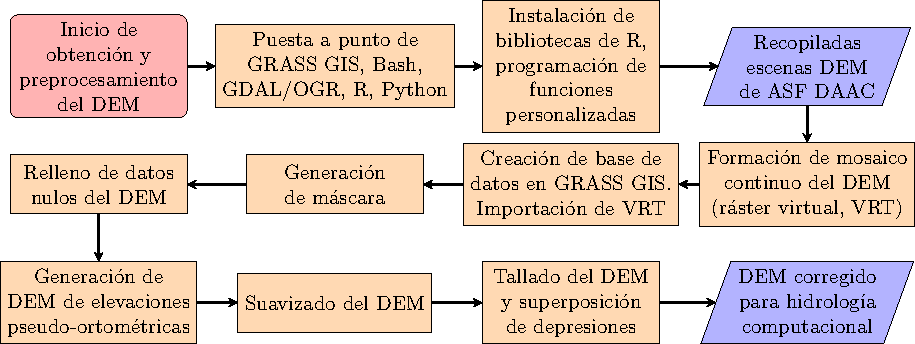
\includegraphics[width=0.8\linewidth]{figuras/resumen-obtencion-preprocesamiento-dem} 

}

\caption{Resumen gráfico de la obtención y preprocesamiento del DEM}\label{fig:obtencionpreprocdem}
\end{figure}

Iniciamos nuestro estudio valorando diversas herramientas para el
procesamiento de los datos (Figura~\ref{fig:obtencionpreprocdem}).
Debido a la gran variedad de complementos que ofrece, junto con su alto
rendimiento y la calidad de los resultados que proporciona, decidimos
utilizar GRASS GIS v8.2.0 para realizar la mayor parte del
preprocesamiento del DEM (GRASS Development Team, 2023). La
implementación de su interfaz de línea de comandos (e.g.~interfaz basada
en texto), en nuestro caso Bash, garantizó la reproducibilidad de
nuestros procedimientos. Nos auxiliamos también de la biblioteca
GDAL/OGR, WhiteboxTools el entorno de programación estadística R y el
lenguaje de programación Python (GDAL/OGR contributors, 2022; Lindsay,
2018; R Core Team, 2023; Van Rossum y Drake, 2009). Nuestro enfoque de
reproducibilidad asegura que, sin importar la fuente de datos empleada,
el seguimiento del flujo de trabajo es viable, manteniendo la integridad
y coherencia del proceso de análisis, sin menoscabo de la calidad del
resultado final.

Asimismo, para facilitar nuestra labor, utilizamos una serie de
bibliotecas de R, además de funciones personalizadas escritas por
nosotros para agilizar y optimizar las tareas de limpieza y
representación de datos y mapas (Hijmans, 2023; O'Brien, 2023; Pebesma,
2018; Pebesma y Bivand, 2023; Tennekes, 2018; Wickham et~al., 2019; Xie,
2014, 2015, 2023; Zhu, 2021). El código reproducible usado en el estudio
se puede consultar en la sección
\protect\hyperlink{infosupl}{Información suplementaria}, así como los
repositorios creados al efecto, donde incluimos el código escrito y las
direcciones para acceder a los datos fuentes, entre otras utilidades.

Nos centramos en la fuente de datos, que en nuestro caso es el modelo
digital de elevaciones (DEM) servido con los productos \emph{Hi-Res
Terrain Corrected} de Alaska Satellite Facility (ASF) (ASF DAAC, 2014).
Este producto se descarga desde el Centro de Archivo Activo Distribuido
del Alaska Satellite Facility o ASF DAAC---una de las instalaciones
temáticas de la Administración Nacional de Aeronáutica y del Espacio de
los Estados Unidos, NASA---en forma de escenas o ``cuadros''
(\emph{tiles}), conteniendo dos imágenes de retrodispersión \(\gamma^0\)
(ca. 70x58 km cada una), una por cada polaridad, y el modelo digital de
elevaciones remuestreado con el que ASF realizó la corrección
radiométrica de terreno (ca. 80x70 km), objeto de nuestro estudio.

Cabe señalar que en un estudio de Aziz y Rashwan (2022), se evaluó la
precisión del DEM comparándolo con otras fuentes de elevación,
encontrándose un rendimiento relativamente bajo en varias pruebas. Sin
embargo, en el trabajo se utilizó el DEM sin preprocesar, lo cual
seguramente afectó el detectado bajo rendimiento. Consideramos que, a
pesar de los resultados de su comparativa, la alta resolución del DEM lo
convierte en una excelente opción para la extracción de redes de
drenaje, siempre que se apliquen filtros apropiados (Ngula Niipele y
Chen, 2019). Además, ASF señaló en su documentación (ASF DAAC, 2014;
JAXA/METI y ASF DAAC, 2015) que el DEM usado en la RTC no es una fuente
confiable de elevación, por lo que el resultado obtenido por Aziz y
Rashwan (2022) era más bien el esperado.

Para conformar un mosaico continuo del DEM de República Dominicana,
seleccionamos y descargamos más de 40 escenas únicas de ALOS-PALSAR
desde el ASF DAAC (JAXA/METI y ASF DAAC, 2015), minimizando la
redundancia espacial y eligiendo las versiones más recientes,
conservando sólo 28 escenas distintas (Figura~\ref{fig:mapaindice} y
Tabla~\ref{tab:tablaindice}). Después, extrajimos los DEM
correspondientes de los archivos comprimidos y transformamos aquellos
proyectos en el huso 18N al 19N del sistema UTM. Posteriormente, creamos
un mosaico continuo (``sin costuras'') usando el formato de ráster
virtual.

\begin{figure}

{\centering 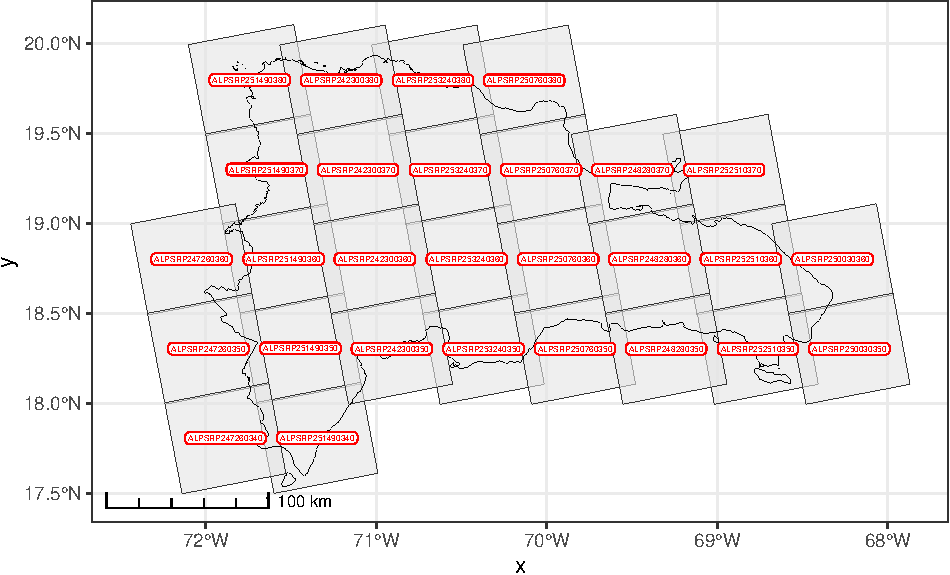
\includegraphics[width=0.8\linewidth]{preprint_files/figure-latex/mapaindice-1} 

}

\caption{Mapa índice de las 28 escenas usadas en la formación del DEM de República Dominicana, superponiendo las huellas (polígono de área con datos) de las escenas ALOS PALSAR RTC sobre el límite costero e internacional del país}\label{fig:mapaindice}
\end{figure}

Posteriormente, creamos una base de datos, con su correspondiente
localización, en GRASS GIS, nuestro software principal por su
eficiencia. Ocasionalmente recurrimos a otras herramientas como
WhiteboxTools y QGIS, siempre con el objetivo de optimizar el uso de los
recursos de hardware para obtener los resultados necesarios de manera
rápida (GRASS Development Team, 2023; Lindsay, 2018; QGIS Development
Team, 2021). Complementariamente, generamos una máscara de país en QGIS,
fusionando el límite oficial de la Oficina Nacional de Estadística con
fuentes en línea como GADM, OCHA y OpenStreetMap, y excluyendo
superficies de lagos naturales y embalses para facilitar el análisis de
cuencas endorreicas; este paso fue realizado de forma semimanual.
Posteriormente, importamos tanto el ráster virtual como la máscara a la
base de datos de GRASS GIS (Figura~\ref{fig:demsinprocesar}).
Inmediatamente, aplicamos la máscara a la región activa para enfocar los
análisis sólo dentro del área de interés. (GADM, 2022; OCHA, 2022;
Oficina Nacional de Estadística (ONE), 2018; OpenStreetMap contributors,
2017; QGIS Development Team, 2021).

Dentro de la base de datos de GRASS, rellenamos los datos nulos del DEM
(Figura~\ref{fig:demrelleno}), para luego suavizar el resultado
preservando morfologías con la herramienta
\emph{FeaturePreservingSmoothing} de WhiteboxTools
(Figura~\ref{fig:demsuavizado}) (Lindsay, 2018; Lindsay et~al., 2019).
Tras esto, combinamos el DEM suavizado con el ráster de altura del
geoide EGM2008 mediante una simple suma algebraica para obtener alturas
pseudo-ortométricas, incrementando previamente la resolución del segundo
para acercarla ligeramente a la del primero.

A continuación, como último paso del preprocesamiento, tallamos el DEM
con una red preexistente de cursos seleccionados de República
Dominicana, un paso clave en la generación de la hidrografía por métodos
computacionales, y que en inglés se conoce como \emph{stream burning}
(Lindsay, 2016). Primero creamos la red a partir de una selección de
ríos permanentes, apoyados en imágenes satelitales (Google; Airbus,
CNES; Airbus, Landsat; Copernicus; Maxar Technologies; U.S. Geological
Survey, 2023), MTN-50K (Instituto Cartográfico Militar (ICM), 1989) y
OpenStreetMap contributors (2017). Para representar ríos que que llenan
embalses, usamos sus trazados históricos para así mantener la
continuidad hidrológica (Figura~\ref{fig:redcursoslargos}). Luego
realizamos el tallado del DEM probando tres algoritmos: \texttt{r.carve}
y \texttt{r.mapcalc} de GRASS GIS, y \texttt{FillBurn} de WhiteboxTools
(GRASS Development Team, 2022a; GRASS Development Team, 2022b, 2022c;
Larson et~al., 1991; Lindsay, 2018; Petrasova et~al., 2011; Saunders,
2000; Shapiro y Westervelt, 1994). Como criterio de selección
establecimos que el mejor algoritmo fuese aquel que lograra una mínima
alteración en el DEM, minimizando a la vez el tiempo de cómputo.
\texttt{r.carve} produjo un buen DEM tallado, aunque ocupó mucho tiempo
de cómputo, por lo que no la consideramos una herramienta adecuada para
iteraciones rápidas. Con \texttt{r.mapcalc} realizamos el tallado
mediante una simple álgebra de mapas (normalización, operaciones
booleanas, multiplicación), de donde obtuvimos un DEM poco alterado en
tiempo relativamente corto. Finalmente, probamos con la función
\texttt{FillBurn} de WhiteboxTools, la cual produjo un DEM tallado
sustancialmente alterado respecto del original, especialmente en las
áreas de karst con depresiones. Optamos por continuar nuestro flujo de
procesamiento con el DEM tallado por \texttt{r.mapcalc} (ver
Figura~\ref{fig:demtallado}).

Finalmente, como último paso del preprocesamiento del DEM, aplicamos
algoritmos para superponer depresiones al modelo, un paso esencial para
dirigir la escorrentía y definir de forma coherente los límites de las
cuencas y redes de drenaje. Utilizamos diversas fuentes para generar un
conjunto de depresiones. Principalmente, a partir de la capa de
litologías de la República Dominicana (Mollat et~al., 2004),
identificamos las calizas con suficiente grado de karstificación.
Además, utilizamos el complemento \texttt{r.geomorphon} para crear una
capa de depresiones (Jasiewicz y Stepinski, 2013)
(Figura~\ref{fig:geomorfonosrd}), y digitalizamos manualmente algunas
depresiones conocidas. Finalmente, intersectamos las tres fuentes de
datos para producir una capa exhaustiva de las depresiones que capturan
la escorrentía superficial (Figura~\ref{fig:depresiones}).

\hypertarget{procesamiento-de-hidrologuxeda-computacional}{%
\subsection{Procesamiento de hidrología
computacional}\label{procesamiento-de-hidrologuxeda-computacional}}

\begin{figure}

{\centering 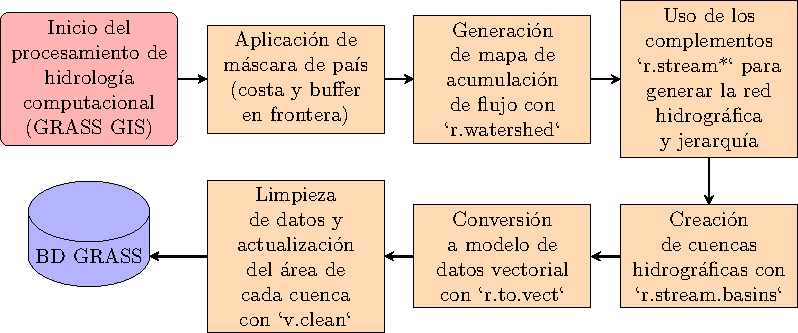
\includegraphics[width=0.8\linewidth]{figuras/resumen-procesamiento-hidrologia-computacional} 

}

\caption{Resumen gráfico del procesamiento de hidrología computacional}\label{fig:procesamientohidrocompu}
\end{figure}

El avance en las técnicas de procesamiento de hidrología computacional
ha permitido estudios cada vez más sofisticados de fenómenos hídricos,
impulsado por las actualizaciones y herramientas disponibles hoy en día,
entre las cuales destacan las de GRASS GIS (Ehlschlaeger, 1989; Freeman,
1991; Holmgren, 1994; Larson et~al., 1991; McCool et~al., 1987; Metz
et~al., 2011; Moore et~al., 1991; Quinn et~al., 1991; Weltz et~al.,
1988). Por su potencial y múltiples complementos disponibles, todo el
procesamiento de hidrología computacional lo desarrollamos en GRASS GIS
(Figura~\ref{fig:procesamientohidrocompu}).

Antes de iniciar el procesamiento de hidrología computacional con GRASS
GIS, aplicamos una máscara de país, delimitada por la línea de costa y a
los límites fronterizos, para evitar que las redes se extendieran más
allá de nuestra área de interés. Posteriormente, generamos el mapa de
acumulación de flujo con el complemento \texttt{r.watershed} (GRASS
Development Team, 2022d) (Figura~\ref{fig:acumyredrwshed}), y utilizamos
este mapa como fuente de los complementos de la familia
\texttt{r.stream*} para el estudio de redes de drenaje y jerarquía
hidrográfica (Jasiewicz y Metz, 2011). Dentro de esta familia se
encuentran \texttt{r.stream.extract}, que usa el mapa de acumulación de
flujo generado por \texttt{r.watershed} para extraer la red,
\texttt{r.stream.order} para calcular la jerarquía hidrográfica,
\texttt{r.stream.basins} para crear cuencas hidrográficas en función de
la referida jerarquía, y \texttt{r.stream.stats} para calcular
estadísticos y parámetros del análisis hortoniano. En consecuencia,
aplicamos estos algoritmos al DEM para generar la hidrografía dominicana
jerarquizada y la delimitación de las cuencas según órdenes, proceso que
sumarizamos a continuación.

Empleando el DEM y el mapa de acumulación creado con
\texttt{r.watershed}, generamos la red hidrográfica usando el
complemento \texttt{r.stream.extract}, enfocándonos en la extracción de
cursos indiferenciados, sin caracterización hidrodinámica, sólo
morfológica (Freeman, 1991; Jasiewicz y Metz, 2011; Marchesini et~al.,
2021). Basándonos en experiencia de terreno y estudios previos,
seleccionamos umbrales de acumulación de 180, 540 y 900 celdas,
equivalentes a 3, 8 y 14 hectáreas respectivamente (Freeman, 1991;
Marchesini et~al., 2021). Automatizamos la generación de las redes con
un bucle \texttt{for} en Bash, iterando sobre cada umbral de
acumulación; para cada red generada
(Figura~\ref{fig:redindiferenciada}), actualizamos la base de datos y
creamos un resumen con estadísticas básicas.

Para determinar la red hidrográfica óptima de alta densidad de República
Dominicana, realizamos una inspección visual de los tres resultados
generados a partir de los umbrales de acumulación elegidos
(Figura~\ref{fig:redorden3umbrales}). Tras evaluar las redes,
seleccionamos la obtenida con el umbral de 540 celdas, por ajustarse a
nuestros criterios de selección. Sin embargo, para preservar la
reproducibilidad de nuestros resultados y facilitar eventuales
aplicaciones futuras, decidimos conservar todos las redes en la base de
datos, incluyendo las originadas a partir de los umbrales de 180 y 900
celdas. En concreto, la red generada con el umbral 180 celdas, presenta
un buen ajuste con las vaguadas topográficas marcadas en el mapa
topográfico, ofreciendo diversas opciones para futuros estudios o
aplicaciones que requieran niveles de resolución más detallados
(Figura~\ref{fig:redordenumbral180}).

A continuación, con el complemento \texttt{r.stream.order} de GRASS GIS,
calculamos la jerarquía de la red hidrográfica para cada uno de los
umbrales de acumulación previamente establecidos (180, 540 y 900
celdas), utilizando un bucle en Bash para automatizar el proceso. Este
análisis permitió obtener la jerarquía de la red hidrográfica de acuerdo
a los métodos de Strahler y Horton, ofreciendo información útil para
nuestros objetivos (Horton, 1945; Strahler, 1957). El resultado obtenido
lo usamos como entrada del complemento \texttt{r.stream.stats} para
obtener los estadísticos básicos de la red hidrográfica según órdenes,
como los promedios de longitudes y pendientes, la densidad de drenaje y
la razón de bifurcación, entre otros.

Utilizando el complemento \texttt{r.stream.basins} de GRASS GIS,
delimitamos las cuencas y subcuencas según la jerarquía de red para cada
uno de los tres umbrales de acumulación. Este proceso permitió la
delimitación de unidades que incluyen, de forma indiferenciada, tanto
cuencas como subcuencas con redes de drenaje tributarias.
Posteriormente, aplicamos el mismo complemento para delimitar las
cuencas que desembocan en el mar, lagos, lagunas o pérdidas del karst,
excluyendo las subcuencas tributarias (e.g.~cuencas sin prolongación de
drenaje superficial fuera de ellas).

Seleccionamos las cuencas generadas para el umbral de 540 celdas y las
convertimos en un modelo de datos vectorial utilizando el complemento
\texttt{r.to.vect} de GRASS GIS, eliminando las cuencas de menos de
4000~m\textsuperscript{2}. Este procedimiento incluyó la creación y
actualización de una nueva columna \texttt{strahler} en la tabla de
atributos de cada capa vectorial para indicar el correspondiente orden
de red. Después de procesar y fusionar todas las cuencas de cada orden
en una única capa vectorial con \texttt{v.patch}, procedimos a limpiar y
preparar los datos para el análisis. Este paso, que incluyó la
corrección de topología, la actualización del área de cada cuenca con
\texttt{v.clean}, la eliminación de áreas espurias y artefactos, resultó
crítico para garantizar la precisión de nuestros resultados. A
continuación, seleccionamos los datos válidos y los exportamos a un
archivo de texto, lo que nos proporcionó valiosas estadísticas del área
para cada cuenca con desembocadura en mares, lagos o en pérdidas
kársticas, según el orden Strahler para nuestro análisis posterior.

Finalizamos la etapa de procesamiento hidrológico utilizando los
complementos \texttt{r.stream.stats} y \texttt{r.accumulate}. Mediante
\texttt{r.stream.stats}, derivamos estadísticas fundamentales de redes y
cuencas clasificadas por órdenes de red. Estas incluyeron medidas como
los promedios de longitud de los cursos, áreas drenadas, pendientes,
gradientes y diferencias de elevación. Además, determinamos la razón de
bifurcación utilizando dos métodos: coeficientes de regresión y
promedios. Por su parte, con \texttt{r.accumulate} generamos los cursos
más largos de aquellos ríos con un alto orden de red, asegurando, a su
vez, una adecuada representatividad territorial.

\hypertarget{resultados}{%
\section{Resultados}\label{resultados}}

La base de datos de cuencas hidrográficas delimitadas y la red de
drenaje extraída usando el umbral de acumulación de 540 celdas
(\textasciitilde8 ha), se ajustó bien a nuestros criterios óptimos de
selección. El modelo de red hidrográfica y la delimitación de cuencas
demostró coherencia, suficiente detalle y una diversidad sustancial a lo
largo del territorio dominicano, especialmente en las áreas de montaña,
proporcionando una representación hidrográfica precisa sin atenuar
patrones de variabilidad. Presentamos a continuación los principales
hallazgos, en forma de resúmenes estadísticos, de las cuencas y sus
redes de drenaje.

\hypertarget{cuencas-que-desembocan-en-mares-lagos-lagunas-o-en-puxe9rdidas-kuxe1rsticas}{%
\subsection{Cuencas que desembocan en mares, lagos, lagunas o en
pérdidas
kársticas}\label{cuencas-que-desembocan-en-mares-lagos-lagunas-o-en-puxe9rdidas-kuxe1rsticas}}

En el caso de las cuencas que desembocan en mares, lagos, lagunas o en
pérdidas kársticas, en total delimitamos 7087 cuencas hidrográficas
(Figura~\ref{fig:cuencasordenestodas}). Predominan cuencas de gran
tamaño y anchura en los valles del Cibao y de San Juan, así como en la
periferia de la plataforma kárstica sudoriental. Por otro lado, las
cuencas medianas y de forma alargada con forma ligeramente ensanchada en
cabecera, tienden a concentrarse a lo largo del borde meridional de la
Cordillera Central y en el karst de la plataforma sudoriental. Las
cuencas más pequeñas, en cambio, se distribuyen de manera más uniforme a
través de los sistemas kársticos y zonas costeras. Entre todas las
cuencas delimitadas, se alcanzó una jerarquía de red máxima de ocho,
condición que sólo se observó en tres cuencas específicas: Yaque del
Sur, Yuna y Ozama.

La cuenca más extensa, correspondiente al río Yaque del Norte, cubre una
superficie de 6986~km\textsuperscript{2}, aunque sólo alcanzó orden
máximo de siete, seguida de las cuencas de los ríos Yuna
(4950~km\textsuperscript{2}) y Yaque del Sur
(4674~km\textsuperscript{2}), ambas con orden máximo de ocho (en la
sección ``Discusión'' abordamos la discrepancia entre las superficies de
cuencas obtenidas por nosotros y los tamaños publicados en referencias
existentes). El tamaño promedio de las cuencas es de
7~km\textsuperscript{2} y desviación estándar de
129~km\textsuperscript{2}, reflejando la diversidad de las cuencas
hidrográficas presentes en el país.

\begin{figure}

{\centering 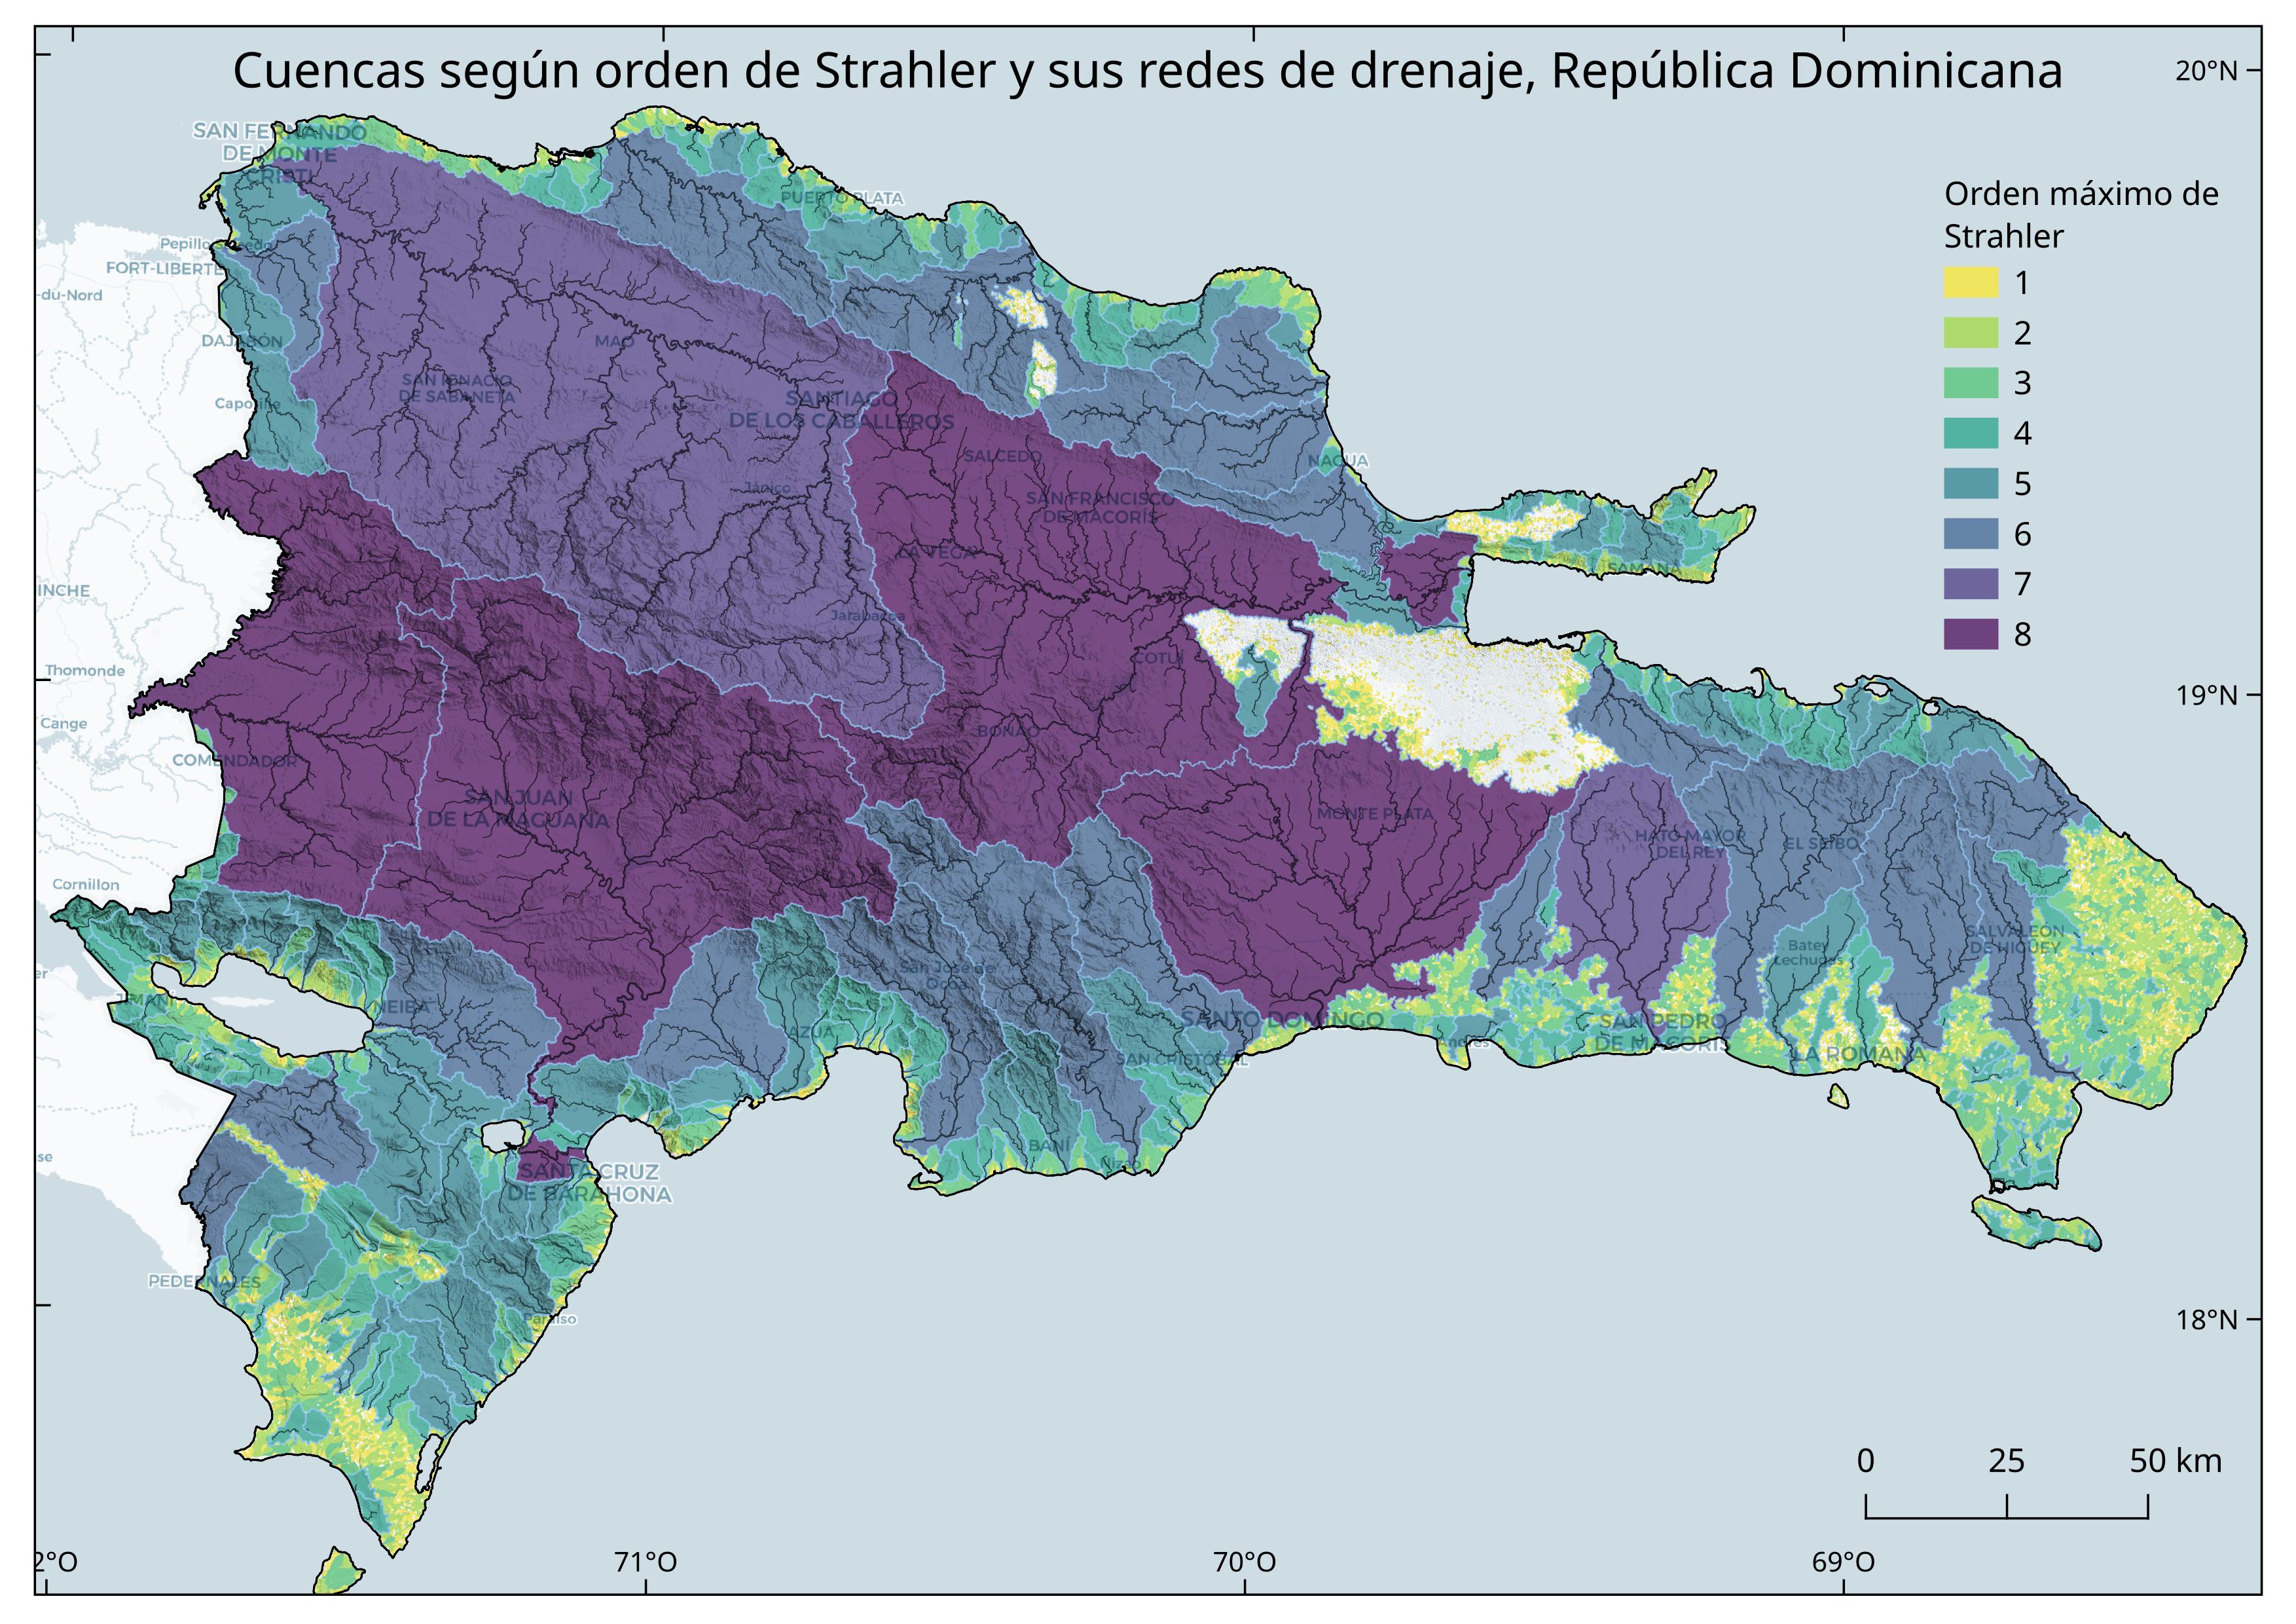
\includegraphics[width=0.8\linewidth]{figuras/cuencas-ordenes-todas} 

}

\caption{Cuencas que desembocan en mares, lagos, lagunas o en pérdidas kársticas categorizadas según orden de Strahler de República Dominicana, y sus correspondientes redes de drenaje (sólo mostrando los cursos de orden 4 o superior). El umbral de acumulación usado para extraer la red fue de 540 celdas (aprox. 8 ha).}\label{fig:cuencasordenestodas}
\end{figure}

La mitad de las cuencas delimitadas tiene 0.36~km\textsuperscript{2} o
menos de superficie, el 25\% de las cuencas más grandes apenas supera
los 0.85~km\textsuperscript{2} y, de hecho, el 5\% más grande sólo
alcanza 5.4~km\textsuperscript{2} o más. Por lo tanto, la distribución
de las cuencas por tamaño es asimétrica hacia la derecha (asimetría
calculada, 40.2), con un importante número de cuencas pequeñas y pocas
grandes, un patrón bastante común en este tipo de conjunto de datos.

\begin{table}[H]

\caption{\label{tab:tablaordenesarea}Orden de red de Strahler y número de cuencas que desembocan en mares, lagos, lagunas o en pérdidas kársticas, para el umbral de acumulación 540 celdas ($\sim$ 8 hectáreas)}
\centering
\begin{tabu} to \linewidth {>{\raggedright}X>{\raggedleft}X>{\raggedleft}X>{\raggedleft}X}
\toprule
Orden de red (Strahler) & Número de cuencas & Área total (km$^2$) & Área promedio (km$^2$) (error est.)\\
\midrule
1 & 4152 & 1095 & 0.2638 (0.002423)\\
2 & 2077 & 1979 & 0.9526 (0.01493)\\
3 & 624 & 2406 & 3.856 (0.1192)\\
4 & 164 & 3541 & 21.59 (1.239)\\
5 & 44 & 4559 & 103.6 (10.94)\\
\addlinespace
6 & 20 & 10130 & 506.7 (55.31)\\
7 & 2 & 7960 & 3980 (3006)\\
8 & 4 & 14970 & 3743 (620)\\
Total & 7087 & 46640 & -\\
\bottomrule
\end{tabu}
\end{table}

Los estadísticos básicos de cuenca sugieren que los resultados obtenidos
fueron consistentes, pues observamos el típico decrecimiento exponencial
del número de cuencas en relación con el orden de red (ver
Figura~\ref{fig:ordennumcuencas} y Tabla~\ref{tab:tablaordenesarea}). En
segundo lugar, destaca un hecho particular reseñable: el número de
cuencas de orden siete es menor que el número de cuencas de orden ocho,
un hecho que afecta a la cuenca del Yaque del Norte que, con
independencia de su gran tamaño, no alcanza la jerarquía máxima.

\begin{figure}

{\centering 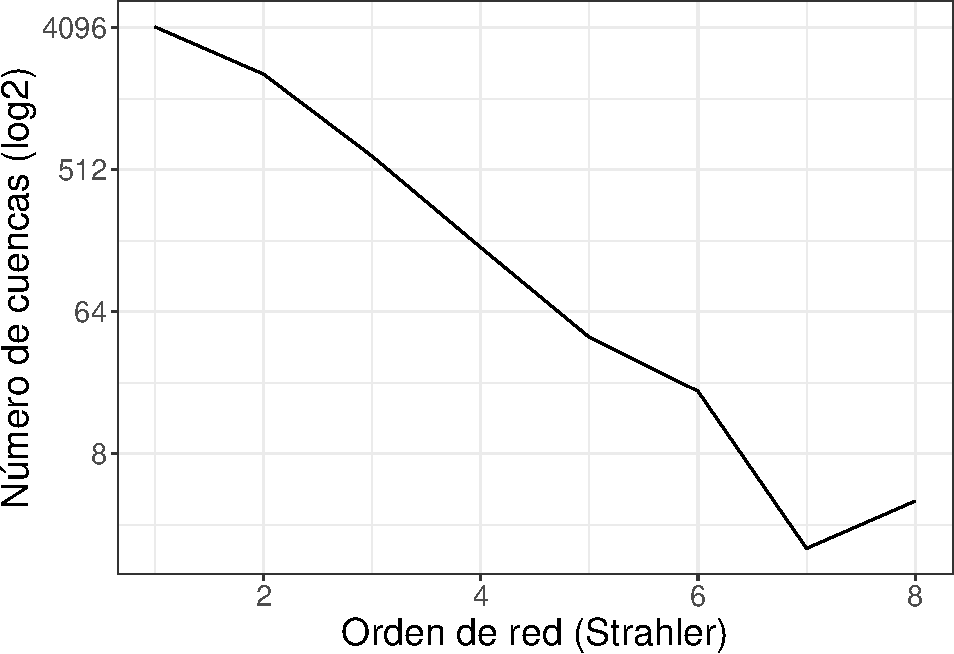
\includegraphics[width=0.6\linewidth]{preprint_files/figure-latex/ordennumcuencas-1} 

}

\caption{Número de cuencas que desembocan en mares, lagos, lagunas o en pérdidas kársticas, según órdenes de red de Strahler para el umbral de acumulación 540 celdas ($\sim$8 hectáreas)}\label{fig:ordennumcuencas}
\end{figure}

Una caracterización de las cuencas que alcanzan un orden cuatro o mayor
resulta también oportuna en este caso, dado que las de orden de red
inferior son muy numerosas y, por la naturaleza del DEM empleado, la
delimitación de las cuencas pequeñas es más propensa a error. Así,
enfocando nuestro análisis sólo en las cuencas de orden cuatro o mayor,
encontramos algunos patrones de interés que merecen mención.

Contabilizamos 234 cuencas de orden cuatro y mayor, lo que representa un
3.3\% del total nacional. Sin embargo, este pequeño porcentaje
representa, en términos de superficie, el 88.3\% del área total de
cuencas. En este subconjunto encontramos un tamaño mínimo de
2.37~km\textsuperscript{2}, promedio de 176~km\textsuperscript{2} y
desviación estándar de 129~km\textsuperscript{2}. La mitad de las
cuencas de orden cuatro y mayor 25.08~km\textsuperscript{2} o menos de
superficie y, aunque este subconjunto de cuencas tiene mejor
distribución, la asimetría a la derecha persiste (asimetría: 7.3).

\hypertarget{cuencas-y-subcuencas}{%
\subsection{Cuencas y subcuencas}\label{cuencas-y-subcuencas}}

Extrajimos las cuencas y subcuencas en función de su orden de red y
calculamos su extensión superficial. En este caso, delimitamos las
unidades hidrográficas de forma desagregada para aportar insumos al
análisis de posibles patrones de asociación con elementos territoriales
y ambientales (Tabla~\ref{tab:tablacuencassubareas} y
Figura~\ref{fig:ordenarecuencas}).

\begin{table}[H]

\caption{\label{tab:tablacuencassubareas}Estadísticos de superficie (en km$^2$) de cuencas y subcuencas según orden de red de Strahler para el umbral de acumulación  540 celdas ($\sim$ 8 hectáreas)}
\centering
\begin{tabu} to \linewidth {>{\raggedright}X>{\raggedleft}X>{\raggedleft}X>{\raggedleft}X>{\raggedleft}X>{\raggedleft}X>{\raggedleft}X>{\raggedleft}X>{\raggedleft}X>{\raggedleft}X}
\toprule
Orden de red & Número & Media (km${^2}$) & Mediana (km${^2}$) & Desv. estándar (km${^2}$) & Mínimo (km${^2}$) & Máximo (km${^2}$) & Rango (km${^2}$) & Sesgo & Curtosis\\
\midrule
1 & 99918 & 0.29 & 0.23 & 0.21 & 0.00 & 3.33 & 3.33 & 2.35 & 9.80\\
2 & 22788 & 1.27 & 1.01 & 0.93 & 0.06 & 11.13 & 11.07 & 2.19 & 8.03\\
3 & 4942 & 5.73 & 4.47 & 4.29 & 0.58 & 36.26 & 35.68 & 2.10 & 6.54\\
4 & 1049 & 26.79 & 21.78 & 18.73 & 2.37 & 132.07 & 129.69 & 1.70 & 3.90\\
5 & 222 & 126.19 & 105.11 & 86.52 & 12.37 & 514.25 & 501.88 & 1.58 & 3.27\\
\addlinespace
6 & 51 & 489.56 & 402.30 & 241.66 & 68.91 & 1031.78 & 962.88 & 0.42 & -0.85\\
7 & 10 & 2042.74 & 1571.14 & 1815.15 & 664.63 & 6985.68 & 6321.06 & 2.69 & 7.78\\
8 & 4 & 3742.74 & 3678.55 & 1240.04 & 2663.91 & 4949.95 & 2286.04 & 0.04 & -5.75\\
\bottomrule
\end{tabu}
\end{table}

Debido a la relación exponencial entre el área y el orden de red, existe
una diferencia significativa en el tamaño de las cuencas dependiendo de
su orden. Las cuencas de orden 1 son considerablemente más pequeñas, con
un tamaño promedio de menos de 4~km\textsuperscript{2}. En contraste,
las cuencas de orden 8 son varios órdenes de magnitud más grandes,
abarcando casi 5000~km\textsuperscript{2} en promedio. En lo que
respecta a su abundancia, el patrón se invierte. Las cuencas de orden 1
son las más frecuentes, contabilizando cerca de 100,000 en total. Por
otro lado, las cuencas de orden 8 son las menos comunes, con solamente
cuatro identificadas en todo el territorio dominicano. Las cuencas, en
todos los órdenes, presentaron una distribución asimétrica de su
superficie calculada, salvo en el caso de las de orden seis, donde se
alcanzó buena simetría.

\begin{figure}

{\centering 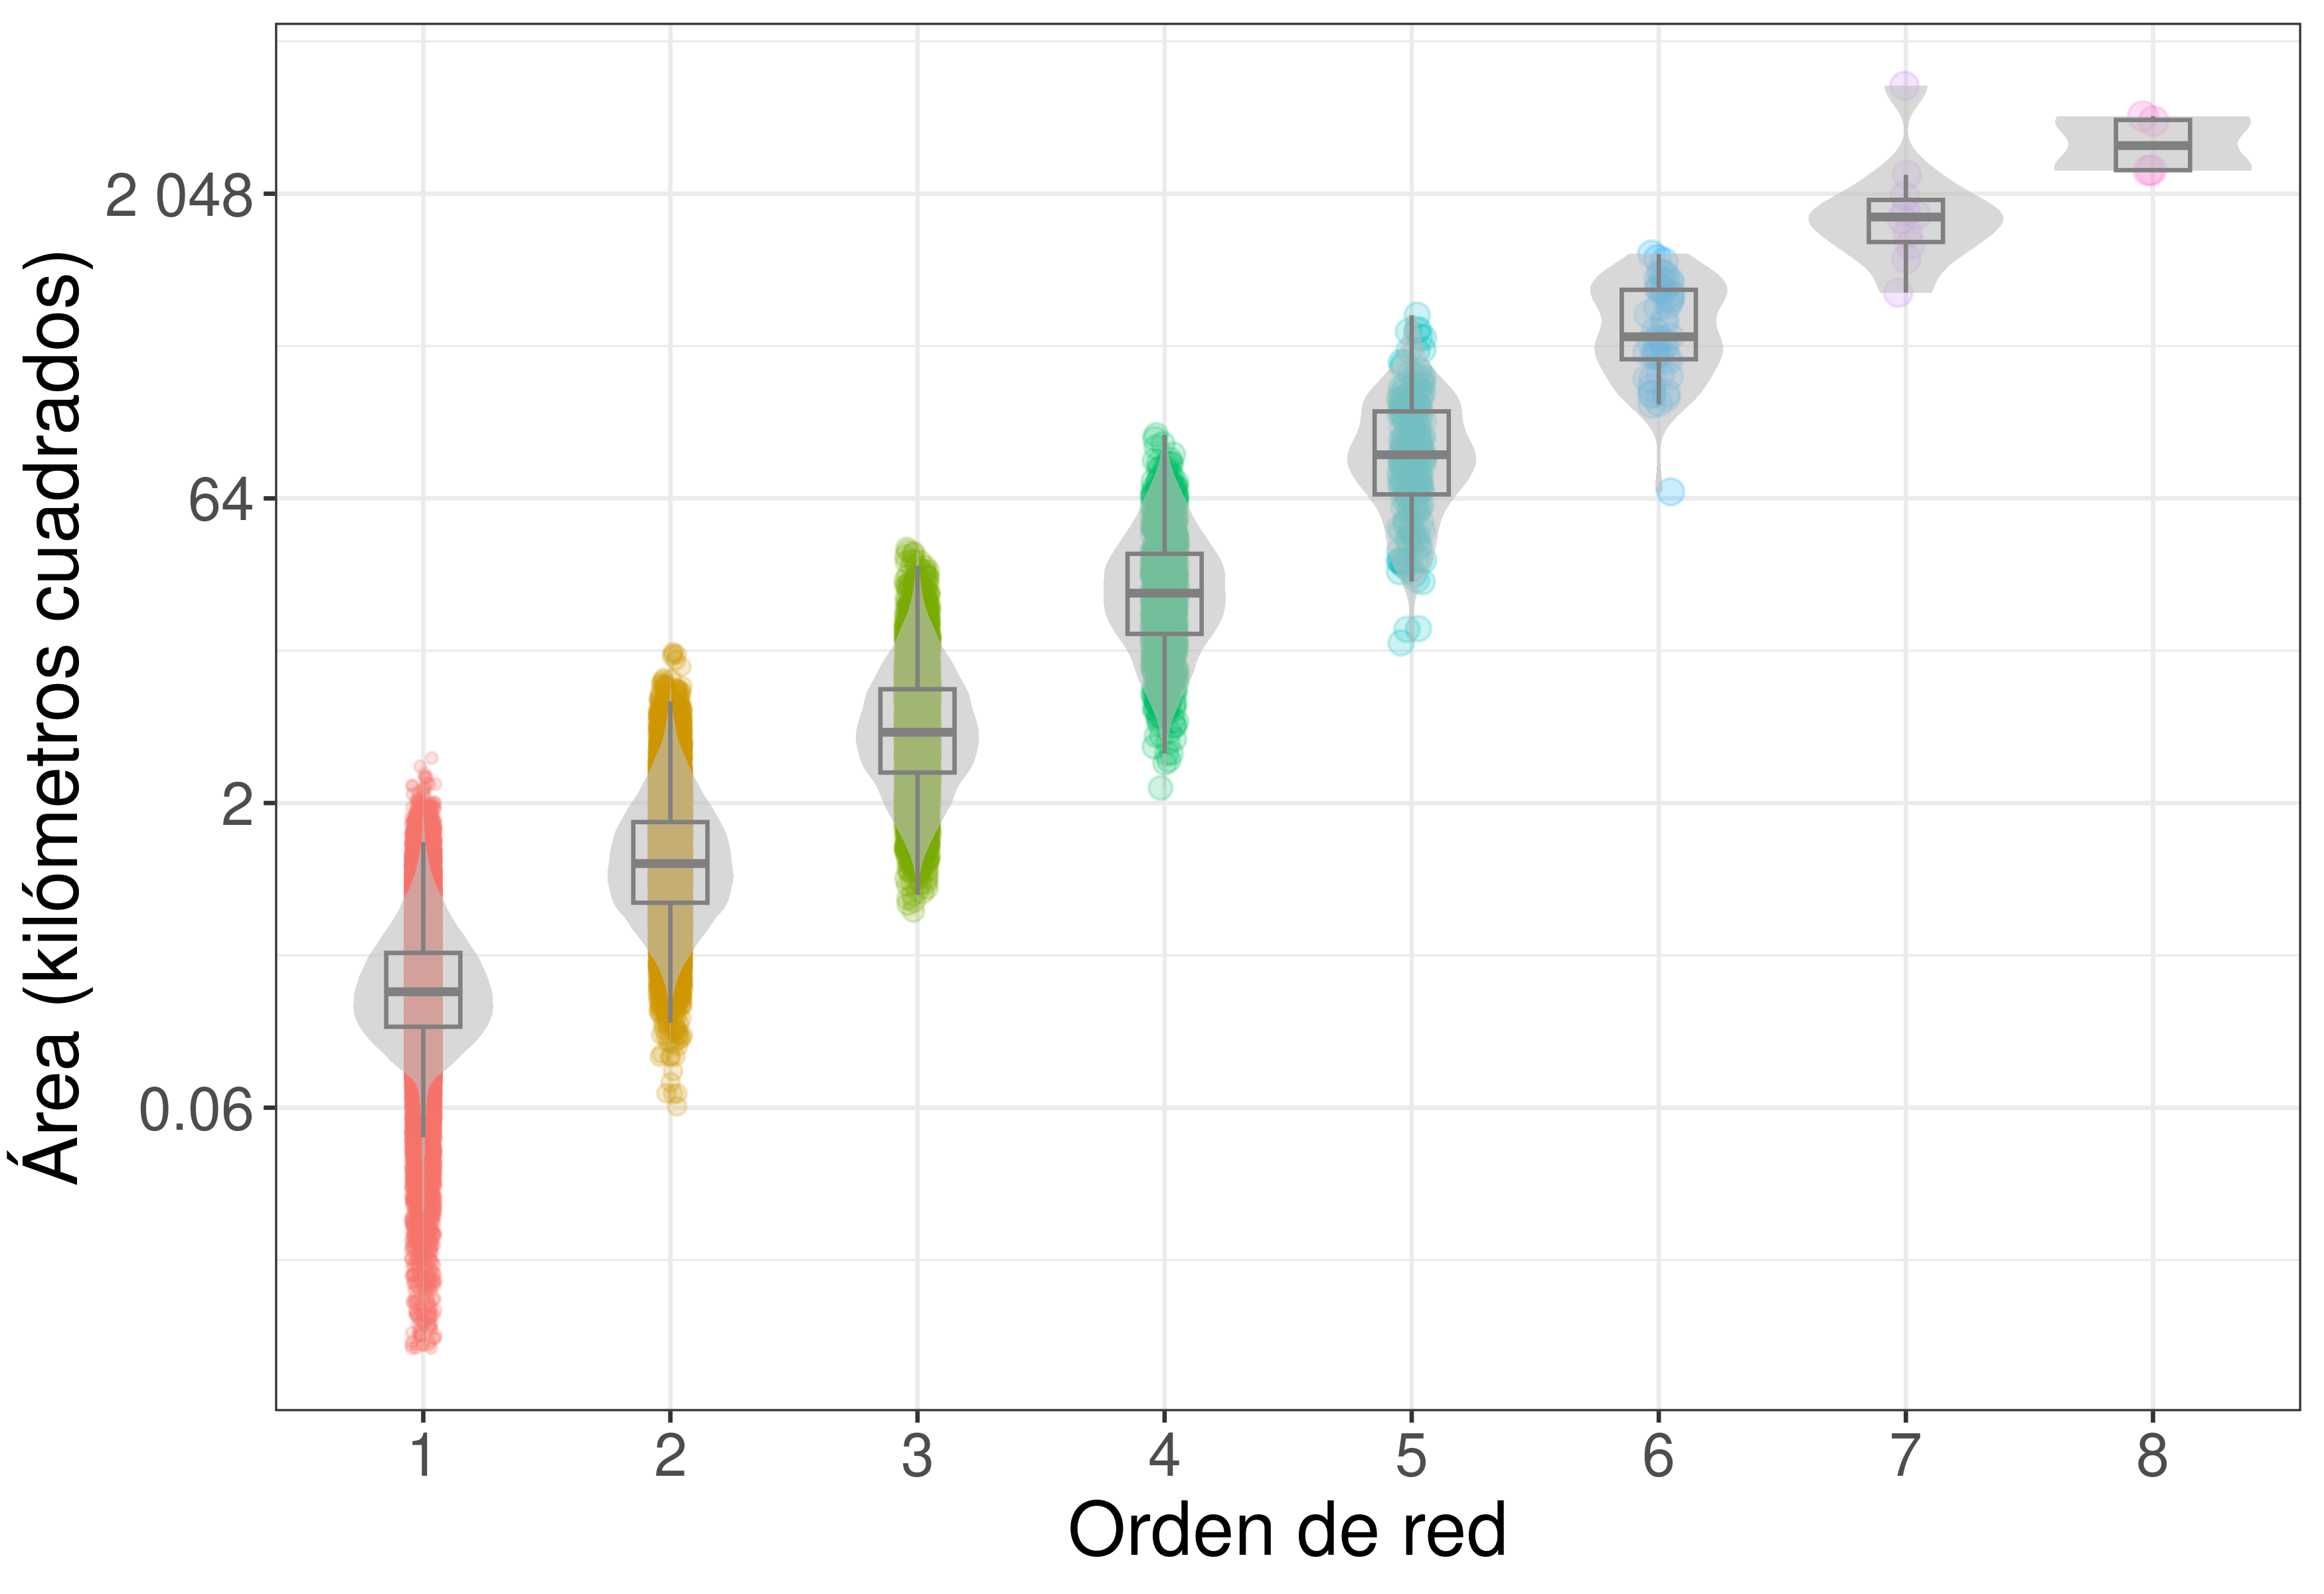
\includegraphics[width=0.8\linewidth]{figuras/cuencas-subcuencas-areas-ordenes-boxplot} 

}

\caption{Área de las cuencas y subcuencas según órdenes de red de Strahler para el umbral de acumulación 540 celdas ($\sim$8 hectáreas)}\label{fig:ordenarecuencas}
\end{figure}

A lo largo de todos los órdenes de red, observamos la presencia de
valores atípicos en las superficies calculadas
(Figura~\ref{fig:ordenarecuencas}). En algunos contextos, estos atípicos
fueron resultado de errores de cómputo o de delimitación de cuencas y
subcuencas, en cuyo caso, corregimos la base de datos eliminando dichas
observaciones. No obstante, hubo casos en los que ciertas cuencas y
subcuencas presentaban dimensiones atípicas genuinas. Un ejemplo notable
es una subcuenca de orden seis, afluente del río Yuna, que se extiende
desde el borde occidental de la península de Samaná. Por otro lado,
respecto a la asimetría, detectamos distribuciones con sesgo hacia la
derecha en todos los órdenes (Tabla~\ref{tab:tablacuencassubareas}). Sin
embargo, el conjunto correspondiente al orden seis destacó al mostrar
una distribución altamente simétrica.

Representamos la distribución espacial de subcuencas según órdenes y
tamaño en el mapa de la Figura~\ref{fig:ordenredcuencasmapa}. Cada uno
de los órdenes obtenidos, del uno al ocho, se encuentra representado en
casi todo el territorio dominicano, especialmente en sus cadenas
montañosas. La mayor parte de las unidades delimitadas son subcuencas,
especialmente las de orden jerárquico inferior, cuyas redes de drenaje
son tributarias de otras subcuencas y cuencas de órdenes mayores.
Analizamos la distribución de las cuencas y subcuencas delimitadas según
órdenes a continuación.

Las subcuencas de los órdenes uno, dos y tres forman cúmulos
particularmente llamativos en los sistemas montañosos, y su distribución
a menudo refleja la orientación general de las estructuras geológicas.
En particular, las subcuencas que son relativamente grandes en su
categoría jerárquica, se reparten de forma dispersa en la cordillera
Central, pero muestran un patrón concentrado en elevaciones altas e
intermedias de las montañas kársticas, incluyendo las sierras de
Bahoruco y Neyba, en los afloramientos de calizas de la cordillera
Oriental, así como en determinados sectores de la cordillera
Septentrional. En esta última, las subcuencas grandes de los órdenes
uno, dos y tres, se concentran en dos áreas clave: a lo largo del eje
principal de la cordillera y en las laderas que rodean la Loma Isabel de
Torres. La concentración de subcuencas grandes de órdenes pequeños en
dichas áreas, pone de relieve la complejidad geológica e hidrológica de
esos terrenos montañosos.

Las subcuencas de orden cuatro, abarcando tamaños desde pequeñas hasta
medianas y grandes, se encuentran ampliamente distribuidas en toda la
República Dominicana. Este grupo presenta características singulares que
detallaremos a continuación. Las grandes destacan generalmente por ser
alargadas y por encontrarse comúnmente orientadas según las estructuras
geológicas, mientras que las medianas y pequeñas tienen mayor razón de
circularidad, y suelen repartirse de forma dispersa, rodeando cúmulos de
cuencas grandes. De manera particular, las subcuencas de orden cuatro
son especialmente abundantes y grandes en todas las vertientes de la
cordillera Central (más escasas al norte), así como en las vertientes
meridionales de la cordillera Oriental y de las sierras de Yamasá y
Bahoruco. Igualmente, destacan cúmulos de cuencas de orden cuatro de
tamaño grande en determinados sectores de la cordillera Septentrional.

En la cordillera Central, las subcuencas grandes de orden cuatro se
concentran en torno a su eje principal noroeste-sudeste, especialmente
en los alrededores de sus máximas elevaciones (Alto Bandera, picos
Duarte y La Pelona), en las vertientes de enlace con los valles altos y
medios (e.g.~Valle de Bao, Valle Nuevo, Constanza, Jarabacoa), dentro
del denominado ``Cinturón de Peralta''---según Hernaiz Huerta y Andrés
(2002), se trata de un sistema de cabalgamientos imbricado con pliegues,
de vergencia hacia el sur, dentro de la denominada cuenca sedimentaria
de Azua---, y en el borde sudoriental, concretamente en niveles medios y
altos de las cuencas de los ríos Nizao, Haina, Nigua.

\begin{figure}

{\centering 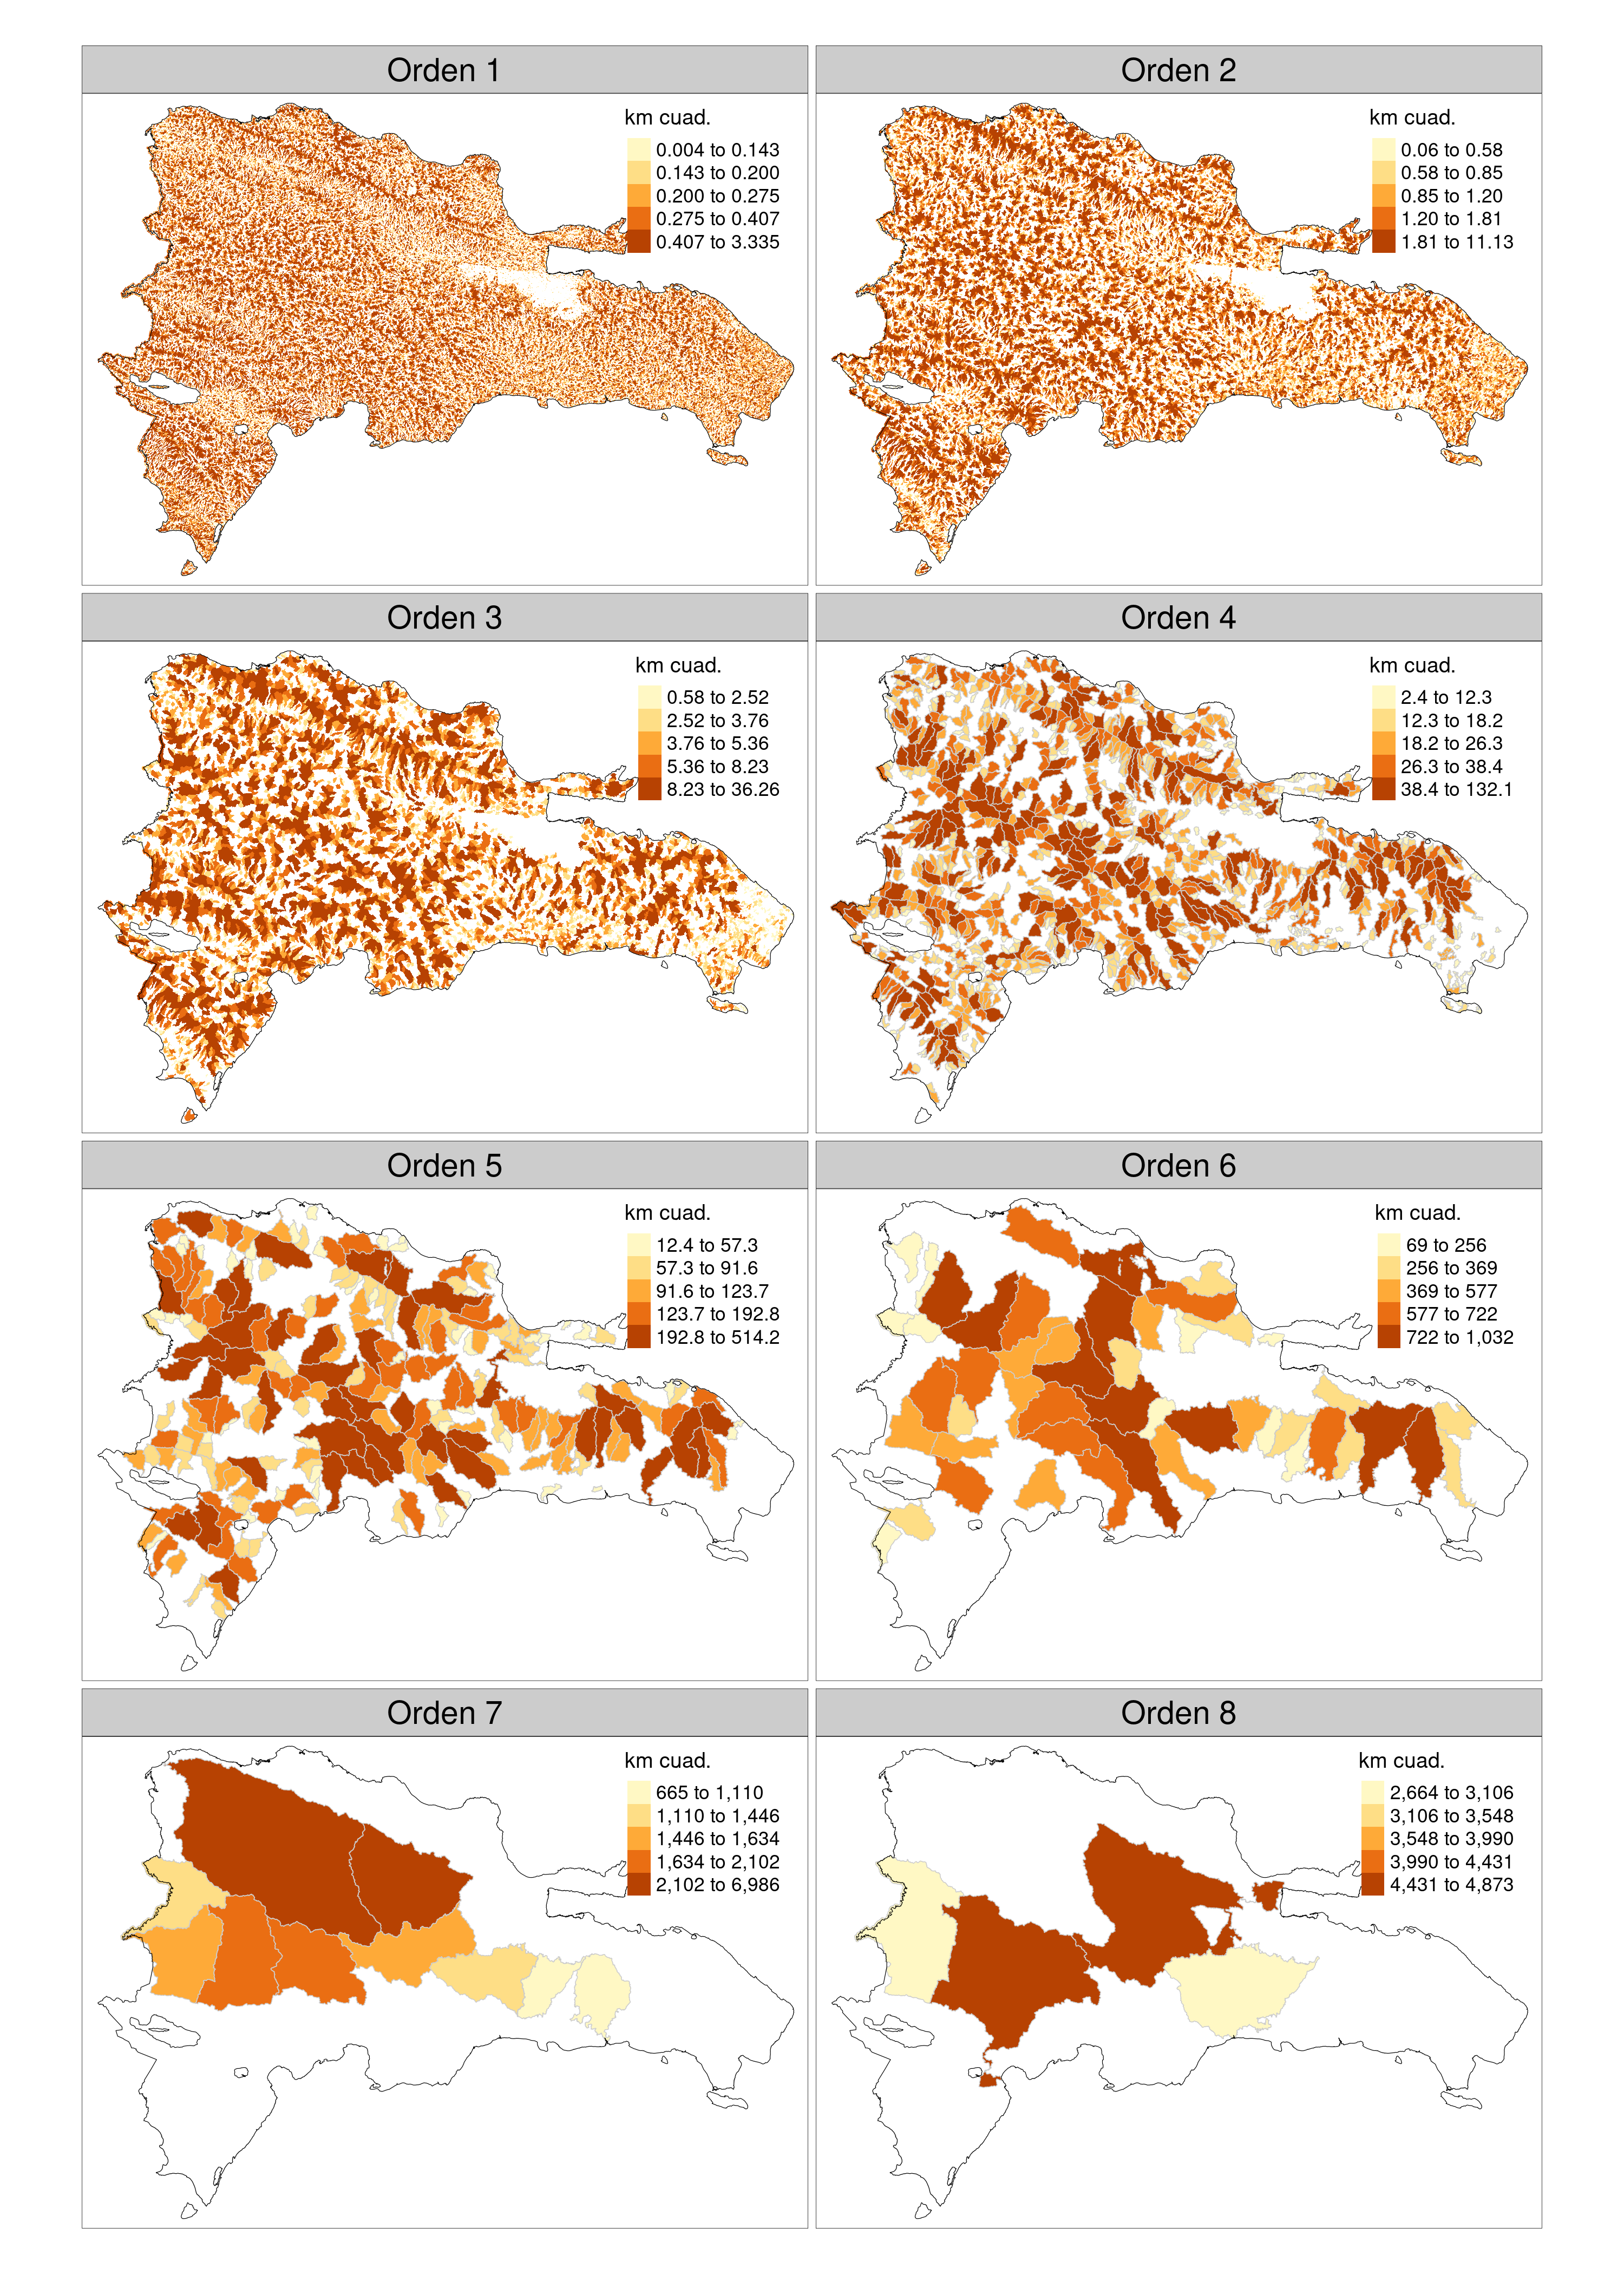
\includegraphics[width=0.8\linewidth]{figuras/cuencas-subcuencas-areas-ordenes} 

}

\caption{Distribución espacial de las cuencas y subcuencas según superficie calculada y órdenes de red de Strahler para el umbral de acumulación 540 celdas ($\sim$8 hectáreas)}\label{fig:ordenredcuencasmapa}
\end{figure}

En la sierra de Yamasá y en la cordillera Oriental, las subcuencas de
orden cuatro, particularmente las grandes, forman cúmulos densos
integrados dentro de cuencas de orden superior, como las del Ozama,
Maguá, Chavón, Cumayasa y Duey. En la sierra de Bahoruco, las subcuencas
de orden cuatro son particulamente grandes en la vertiente sur, en
concreto en el subsistema denominado ``Bahoruco Occidental''---según
Martínez-Batlle (2012), se trata de un sistema montañoso de morfologías
de superficies corrosivas Fini-Paleógenas y Fini-Pliocenas labradas
sobre calizas Cenozoicas, escalonadas desde 2200 m hasta los 100 m---y
hacia el enlace con el Hoyo de Pelempito---uno de los más conocidos
\emph{poljes} dominicanos. En este caso, se trata de cuencas sin cursos
fluviales permanentes, en las que la infiltración logra abrirse paso a
través del karst. Finalmente, las cuencas de orden cuatro en la
cordillera septentrional, se localizan especialmente en los niveles
intermedios y altos de la cuenca del río Bajabonico, así como hacia al
norte de las ciudades de Santiago, Salcedo y San Francisco de Macorís.
Destaca particularmente la alargada subcuenca de orden cuatro del río
Nagua, con casi 130~km\textsuperscript{2}, la cual sigue el rumbo
predominante---noroeste-sudeste---de la Falla Septentrional.

Las cuencas y subcuencas pertenecientes a los órdenes cinco y seis
exhiben patrones de distribución espacial notablemente parecidos entre
sí. Varias unidades de estos órdenes son cuencas propiamente, cuyo curso
principal desemboca comúnmente en el Mar Caribe, el Oceáno Atlántico o
el Lago Enriquillo. Algunos ejemplos de cuencas de orden seis son las de
los ríos Nizao, Haina, Ocoa, Soco, Chavón), y algunas de orden cinco son
las de los ríos Nigua, Cumayasa, Nizaíto, Jura, Duey. Asimismo, por su
tamaño, destacan algunas subcuencas en la vertiente norte y oriental de
la cordillera Central, las cuales encierran redes tributarias de los
ríos Yaque del Norte y Yuna. Es importante subrayar que las cuencas
medianas y grandes de estos órdenes muestran consistentemente una forma
alargada, siguiendo en la mayoría de los casos la orientación de las
estructuras geológicas predominantes.

Por último, caracterizamos las unidades hidrográficas delimitadas como
de órdenes siete y ocho. Estas muestran una concentración espacial
significativa, junto con una amplia variación en términos de tamaño. En
el orden siete delimitamos diez unidades, de las cuales sólo las
correspondientes a los ríos Yaque del Norte e Higuamo califican
propiamente como cuencas, ya que son las únicas que tienen
desembocaduras directas al mar. La cuenca del río Yaque del Norte es
particularmente importante en República Dominicana, pues es la más
grande en términos de superficie, y porque cuenta con múltiples
infraestructuras orientadas a la producción de agua potable y de riego,
así como a la generación hidroeléctrica. No obstante, es notable el
hecho de que esta cuenca, siendo la más grande del país, sólo haya
alcanzado el orden siete. También es destacable el hecho de que la
cuenca del río Higuamo haya alcanzado este orden.

\begin{figure}

{\centering 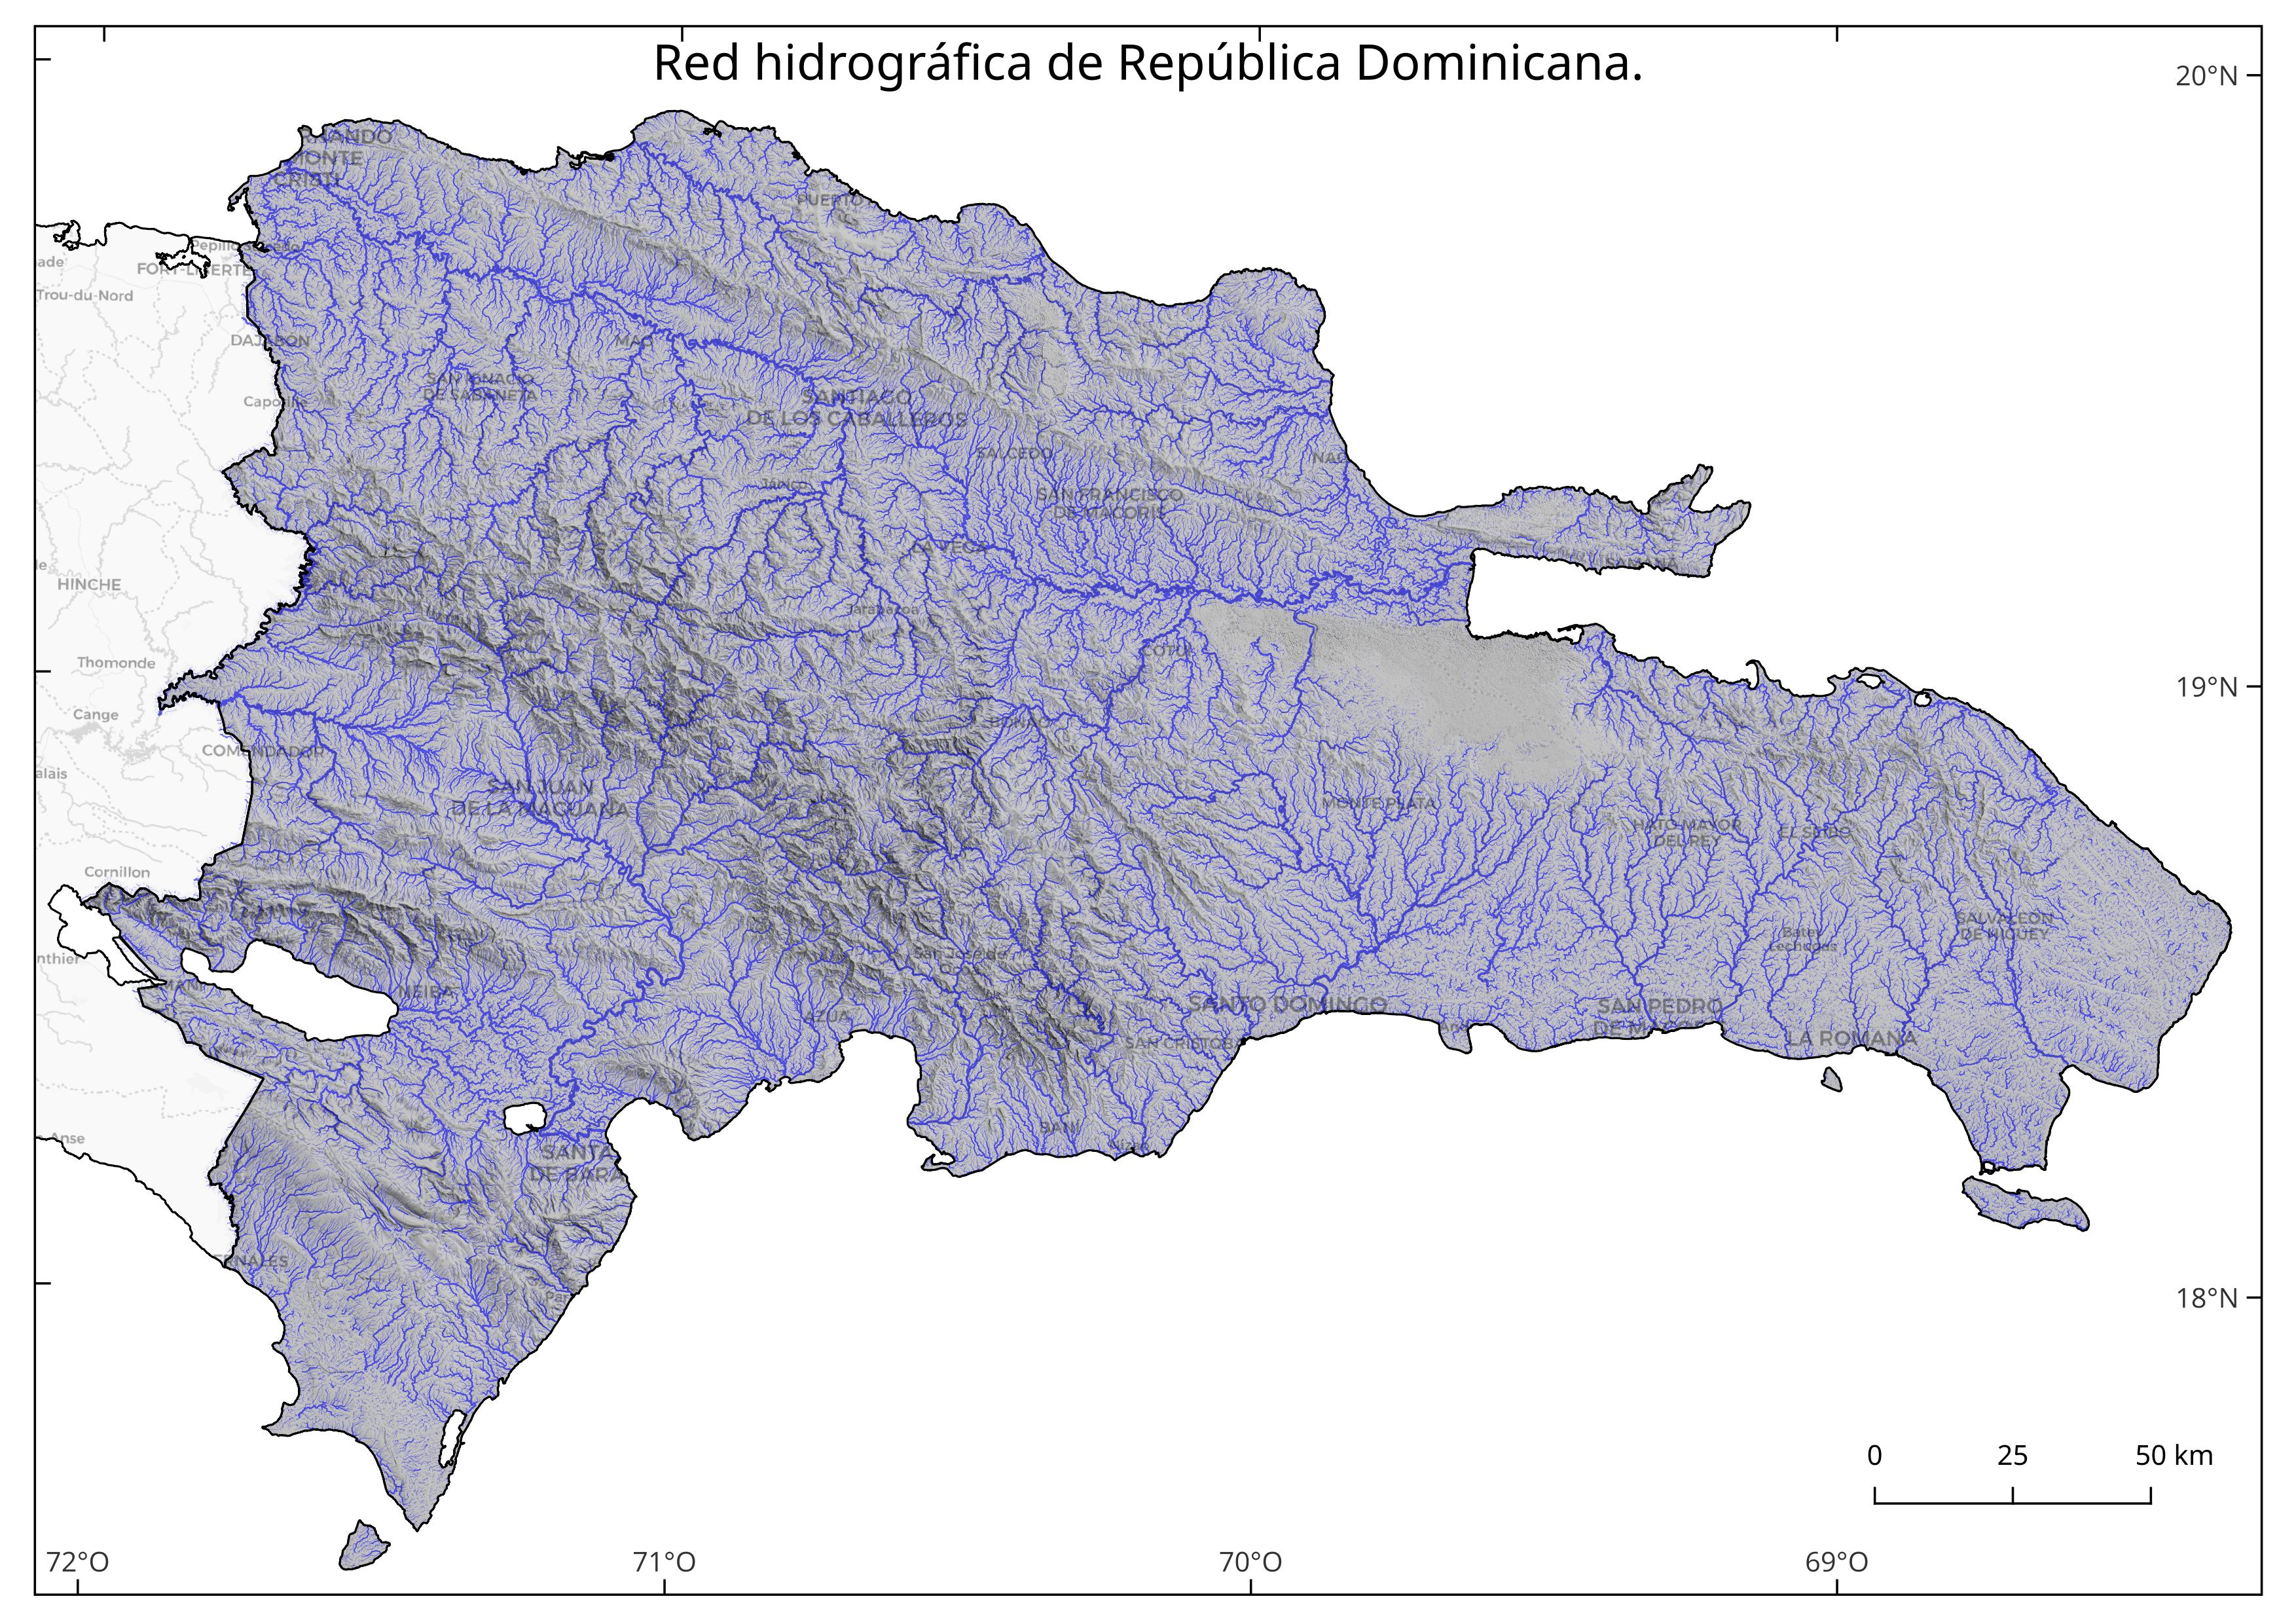
\includegraphics[width=0.8\linewidth]{figuras/red-orden-nacional} 

}

\caption{Representación de la red hidrográfica dominicana simbolizando el grosor de los segmentos en función de su orden de red (método de Strahler). El orden máximo alcanzado fue de 8. Esta red fue generada usando un umbral de acumulación de 540 celdas ($\sim$8 ha)}\label{fig:redordennacional}
\end{figure}

Finalmente, caracterizamos las unidades hidrográficas identificadas como
de órdenes siete y ocho, cuyas particularidades incluyen una notable
concentración espacial y una diversidad considerable en sus dimensiones.
Dentro del orden siete, distinguimos diez unidades, pero sólo las
correspondientes a los ríos Yaque del Norte e Higuamo cumplen con las
características completas de cuencas, dada su condición de contener
desembocaduras directas al mar. Especial mención merece la cuenca del
río Yaque del Norte, por su relevancia en la República Dominicana. Esta
se destaca por ser la de mayor superficie en el país, y por albergar
múltiples infraestructuras esenciales para la producción de agua
potable, riego y generación de energía hidroeléctrica. Sin embargo, es
interesante observar que, a pesar de ser la cuenca más extensa del país,
su jerarquía sólo alcanza el orden siete, quedando por detrás de otras
cuencas que sí alcanzan el orden ocho. Resulta igualmente notable que la
cuenca del río Higuamo, con un tamaño mucho menor (un orden de magnitud
más pequeña), haya alcanzado este mismo orden.

En cuanto a las cuencas de orden ocho, delimitamos sólo cuatro. En este
grupo se incluyen las cuencas del río Yaque del Sur y del Yuna, que son
las número segunda y tercera en tamaño para todo el país,
respectivamente. Las otras dos cuencas son las del río
Artibonito---curso fluvial fronterizo que, al confluir con el Macasías,
adquiere el orden ocho---y la del Ozama. La red fluvial del Artibonito
podría alcanzar un orden máximo superior a ocho si se analizara su
cuenca completa, como bien comentamos en la sección de Metodología.
Destacamos a la cuenca del río Ozama como una singularidad entre las
cuencas listadas dentro de este orden jerárquico, pues se trata de una
cuenca relativamente pequeña, pero con una red bastante ramificada. Con
sus 270~km\textsuperscript{2} calculados en este estudio, es la cuenca
más pequeña de mayor orden de todo el país.

\hypertarget{red-de-drenaje}{%
\subsection{Red de drenaje}\label{red-de-drenaje}}

La red de drenaje de República Dominicana exhibe una variabilidad
notable en sus órdenes jerárquicos, lo que se manifiesta en la
heterogeneidad de su distribución espacial y topográfica. Esta
complejidad en la jerarquía hidrográfica puede apreciarse en la
Figura~\ref{fig:redordennacional}, en la cual se observan distintas
densidades de drenaje según territorios, con mayores concentraciones de
\emph{talwegs} en la vertiente meridional de la cordillera Central y en
la cordillera Septentrional. En los grandes valles, la dirección
predominante de los grandes cursos fluviales es noroeste-sudeste y la
red complementaria es ortogonal. En la cordillera Oriental y en el
enlace hacia el karst de plataforma del sudeste, la dirección
predominante es norte-sur. Destaca igualmente la ausencia de drenaje
superficial en los sistemas kársticos de Los Haitises, y en sectores de
la sierra de Bahoruco y la cordillera Septentrional.

Extrajimos más de 129000 \emph{talwegs} , los cuales alcanzaron una
longitud de poco más de 98000~km (Tabla~\ref{tab:tablaredesordtotales}).
El análisis hortoniano y la caracterización hidrográfica por órdenes de
red según el método de Strahler, proporcionaron información valiosa
sobre la estructura y organización de los sistemas fluviales
dominicanos. El orden jerárquico más alto alcanzado fue ocho, visible en
tramos bien extendidos de los ríos Yuna y Yaque del Sur. Asimismo, un
tramo bajo del río Ozama justo aguas abajo de su confluencia con el
Yabacao, alcanzó el orden este orden máximo, así como en un pequeño
segmento del sistema Macasía-Artibonito situado justo en la confluencia
de ambos ríos. El río dominicano más largo, el Yaque del Norte, sólo
alcanzó el orden jerárquico siete, justo aguas abajo de los ríos Bao,
Jagua y Guanajuma, los cuales confluyen en el embalse de Bao. Otro río
que alcanzó el orden siete, aunque con un tamaño mucho menor que el
Yaque del Norte, fue el Higuamo, justo aguas abajo de la confluencia con
uno de sus más importantes tributarios, el río Maguá.

\begin{table}[H]

\caption{\label{tab:tablaredesordtotales}Totales de número de cursos y longitudes de cursos según órdenes de Strahler de la red generada}
\centering
\begin{tabular}[t]{lrr}
\toprule
Orden de red & Número de cursos & Longitud total (km)\\
\midrule
1 & 100126 & 49627.78\\
2 & 22790 & 24469.96\\
3 & 4942 & 12267.06\\
4 & 1049 & 6381.46\\
5 & 222 & 3329.86\\
\addlinespace
6 & 51 & 1362.22\\
7 & 10 & 599.50\\
8 & 4 & 257.31\\
Total & 129194 & 98295.14\\
\bottomrule
\end{tabular}
\end{table}

Los cursos de órdenes pequeños---e.g., del uno al cuatro---suman un
total de 128907 cursos, casi la totalidad de todos los cursos (en
número), mientras que en longitud suponen 92746~km (94\%). Estos cursos
de órdenes pequeños, especialmente los de los órdenes uno y dos, se
concentran en áreas de montaña, especialmente en sectores de cabecera,
cuencas vertiente y áreas de captación, siendo escasos en las grandes
llanuras y valles bajos. Son especialmente densos en redes de drenaje
del sudoeste, especialmente en el área del denominado ``Cinturón de
Peralta'', asi como en las vertientes altas de la cordillera
Septentrional.

Numerosos ríos dominicanos alcanzaron órdenes de cinco y seis,
concentrados especialmente los valles intramontanos y en los piedemontes
de los sistemas montañosos dominicanos, justo en el enlace con los
grandes valles bajos. Destacan especialmente los tramos de ríos situados
en los piedemontes septentrional y meridional de la cordillera Central,
justo en los enlaces con los valles del Cibao (afluentes del Yaque del
Norte) y de San Juan (tributarios del Yaque del Sur). También son
comunes los cursos de órdenes cinco y seis en el borde meridional de la
cordillera Central, específicamente en el sector que enlaza con el Mar
Caribe, entre los que destacan los ríos Nizao, Ocoa, Haina, Nigua, Jura
y Tábara. Asimismo, varios ríos que nacen en la cordillera Oriental, y
que desembocan en el Mar Caribe, pertenecen a los órdenes cinco y seis,
entre los que merecen mención los ríos Yuma, Chavón, Cumayasa y Soco.
También en este sector se encuentra el río Brujuelas, de orden máximo
seis, el cual se pierde, a través de un conjunto de \emph{ponors},
dentro del karst de plataforma del sudeste dominicano. Por otra parte,
varios sistemas fluviales de la cordillera Septentrional alcanzaron el
orden seis, como son el Boba, Bacuí, Yásica y Bajabonico. Finalmente,
algunos ríos o cursos temporales que desembocan en el Lago Enriquillo
son de orden seis, como el Panzo y Las Damas.

\begin{figure}

{\centering 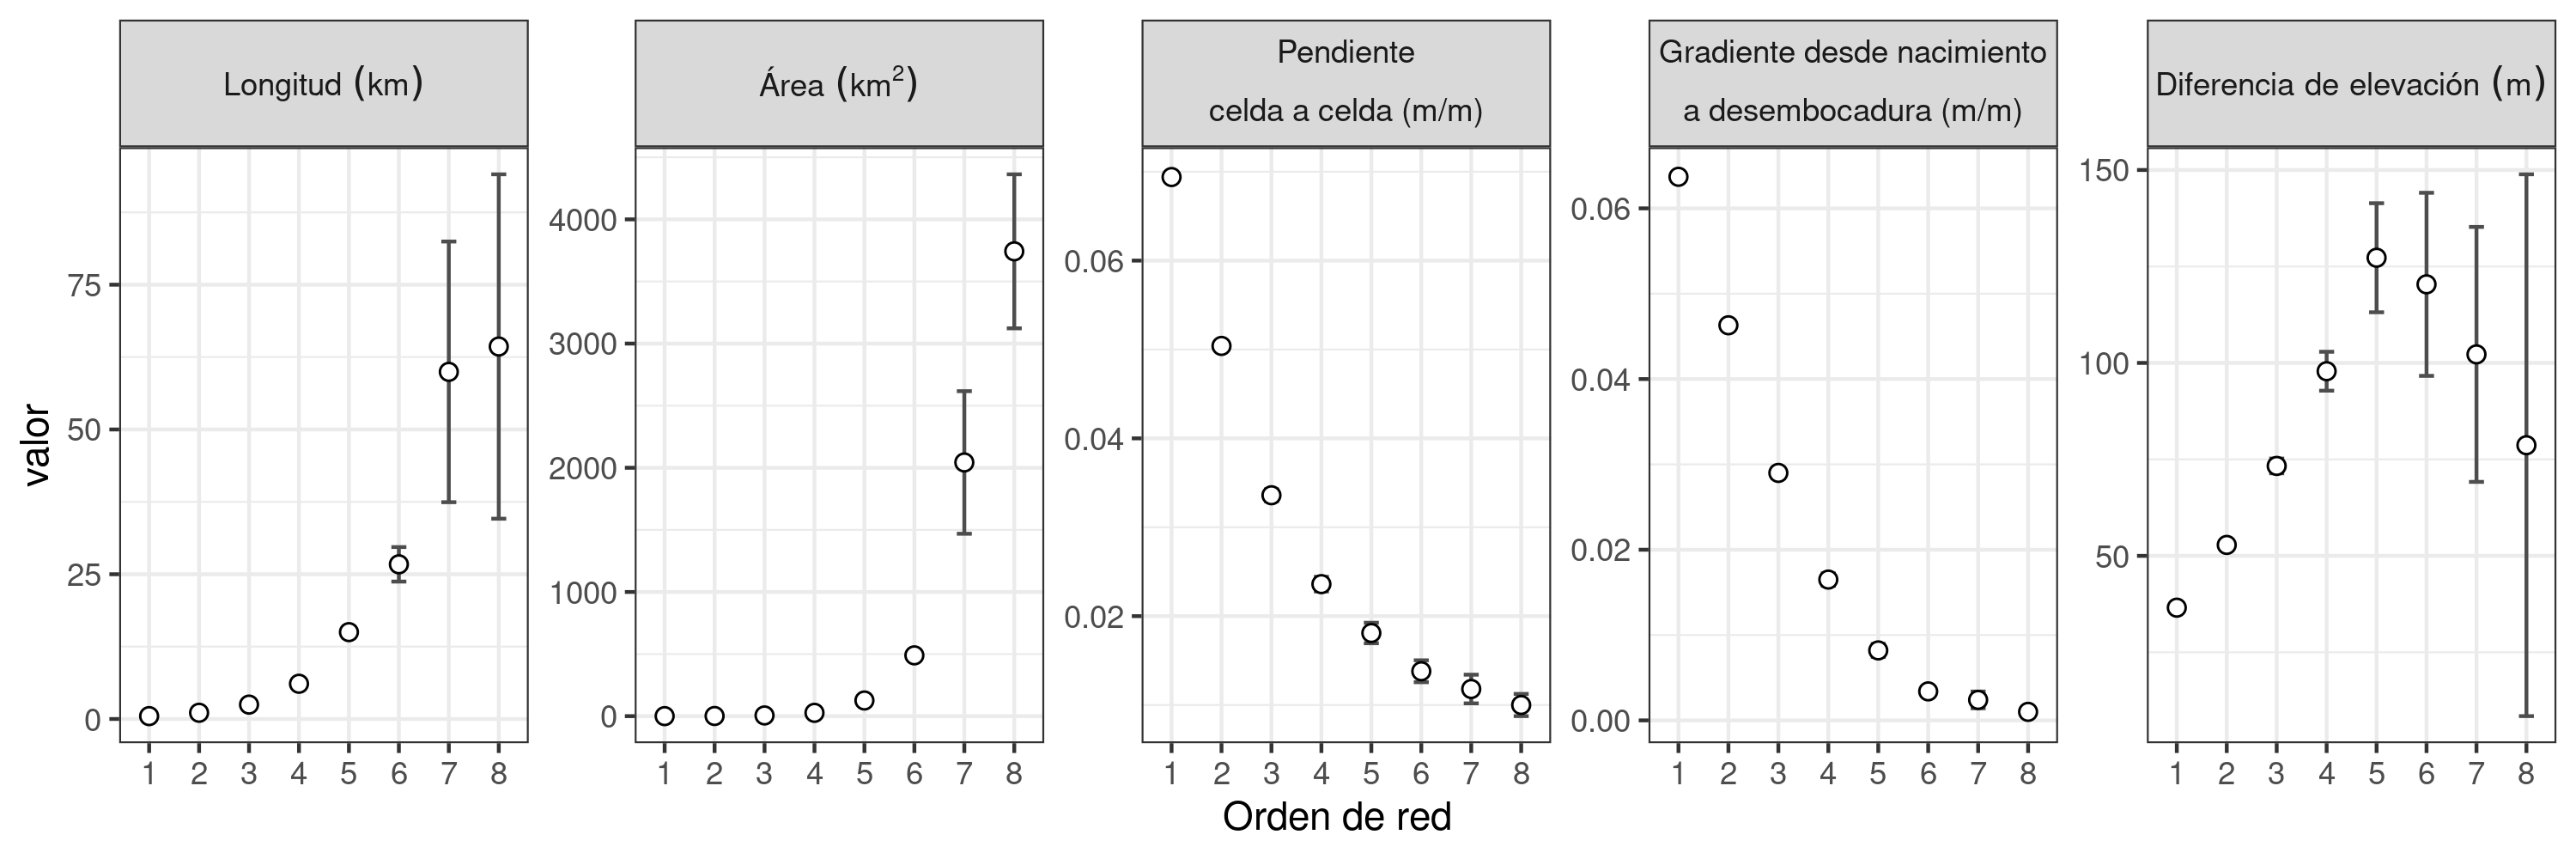
\includegraphics[width=1\linewidth]{figuras/variables-de-redes-segun-ordenes} 

}

\caption{Promedios de longitud de cursos, área de cuenca, pendiente (celda a celda), gradiente (entre extremos) y rango promedio (diferencia de elevación), por tramos, según órdenes de Strahler}\label{fig:variablesredesordenes}
\end{figure}

También analizamos la morfometría de la red hidrográfica en función del
orden de red (Tabla~\ref{tab:tablaredesordpromedios}). Específicamente,
evaluamos los promedios de las siguientes cinco variables por tramos de
cursos fluviales: longitud (km), área de cuenca (km\(^2\)), pendiente
(celda a celda, m/m), gradiente (desde nacimiento a desembocadura, m/m)
y diferencia de elevación (m). Los valores de cada variable incluyen una
estimación del error estándar como medida de dispersión (ver
Figura~\ref{fig:variablesredesordenes} y
Tabla~\ref{tab:tablaredesordpromedios}).

\begin{table}

\caption{\label{tab:tablaredesordpromedios}Promedios y errores estándar (entre paréntesis) de longitud, área de cuenca, pendiente (celda a celda), gradiente (entre extremos) y rango promedio (diferencia de elevación), por tramos, según órdenes de Strahler.}
\centering
\begin{tabu} to \linewidth {>{\raggedright\arraybackslash}p{1cm}>{\raggedleft}X>{\raggedleft}X>{\raggedleft}X>{\raggedleft}X>{\raggedleft}X}
\toprule
Orden de red & Longitud (km) & Área (km$^2$) & Pendiente (m/m) & Gradiente (m/m) & Diferencia de elevación (m)\\
\midrule
1 & 0.5 (0.001) & 0.29 (7e-04) & 0.069 (3e-04) & 0.064 (3e-04) & 37 (0.2)\\
2 & 1.1 (0.007) & 1.3 (0.006) & 0.05 (5e-04) & 0.046 (5e-04) & 53 (0.7)\\
3 & 2.5 (0.03) & 5.7 (0.06) & 0.034 (7e-04) & 0.029 (6e-04) & 73 (2)\\
4 & 6.1 (0.2) & 27 (0.6) & 0.024 (8e-04) & 0.016 (7e-04) & 98 (5)\\
5 & 15 (0.9) & 130 (6) & 0.018 (0.001) & 0.0082 (8e-04) & 130 (10)\\
\addlinespace
6 & 27 (3) & 490 (30) & 0.014 (0.001) & 0.0034 (5e-04) & 120 (20)\\
7 & 60 (20) & 2000 (600) & 0.012 (0.002) & 0.0024 (0.001) & 100 (30)\\
8 & 64 (30) & 3700 (600) & 0.01 (0.001) & 0.001 (5e-04) & 79 (70)\\
\bottomrule
\end{tabu}
\end{table}

El patrón observado en los promedios de longitud y área drenada sigue
una relación exponencial directa con el orden de la red
(Figura~\ref{fig:variablesredesordenes}). Además, la variabilidad de
estas métricas se intensifica en los órdenes de red más altos, siendo
especialmente notable en los órdenes siete y ocho. Para los órdenes de
red del uno al cuatro, las longitudes promedio fluctúan entre 0.5 y
6.1~km, mientras que las áreas promedio oscilan entre 0.29 y
27~km\(^2\), promedios muy bajos en comparación con los correspondientes
a los órdenes de red más altos. Notamos que se produce una inflexión
notable en los promedios de los órdenes cinco y seis, antes de
alcanzarse las longitudes y superficies promedio máximas en los órdenes
siete y ocho. En particular, las longitudes rondan los 60~km, mientras
que las áreas se sitúan entre 2043 y 3743~km\(^2\) para estos órdenes de
red.

\begin{figure}[H]

{\centering 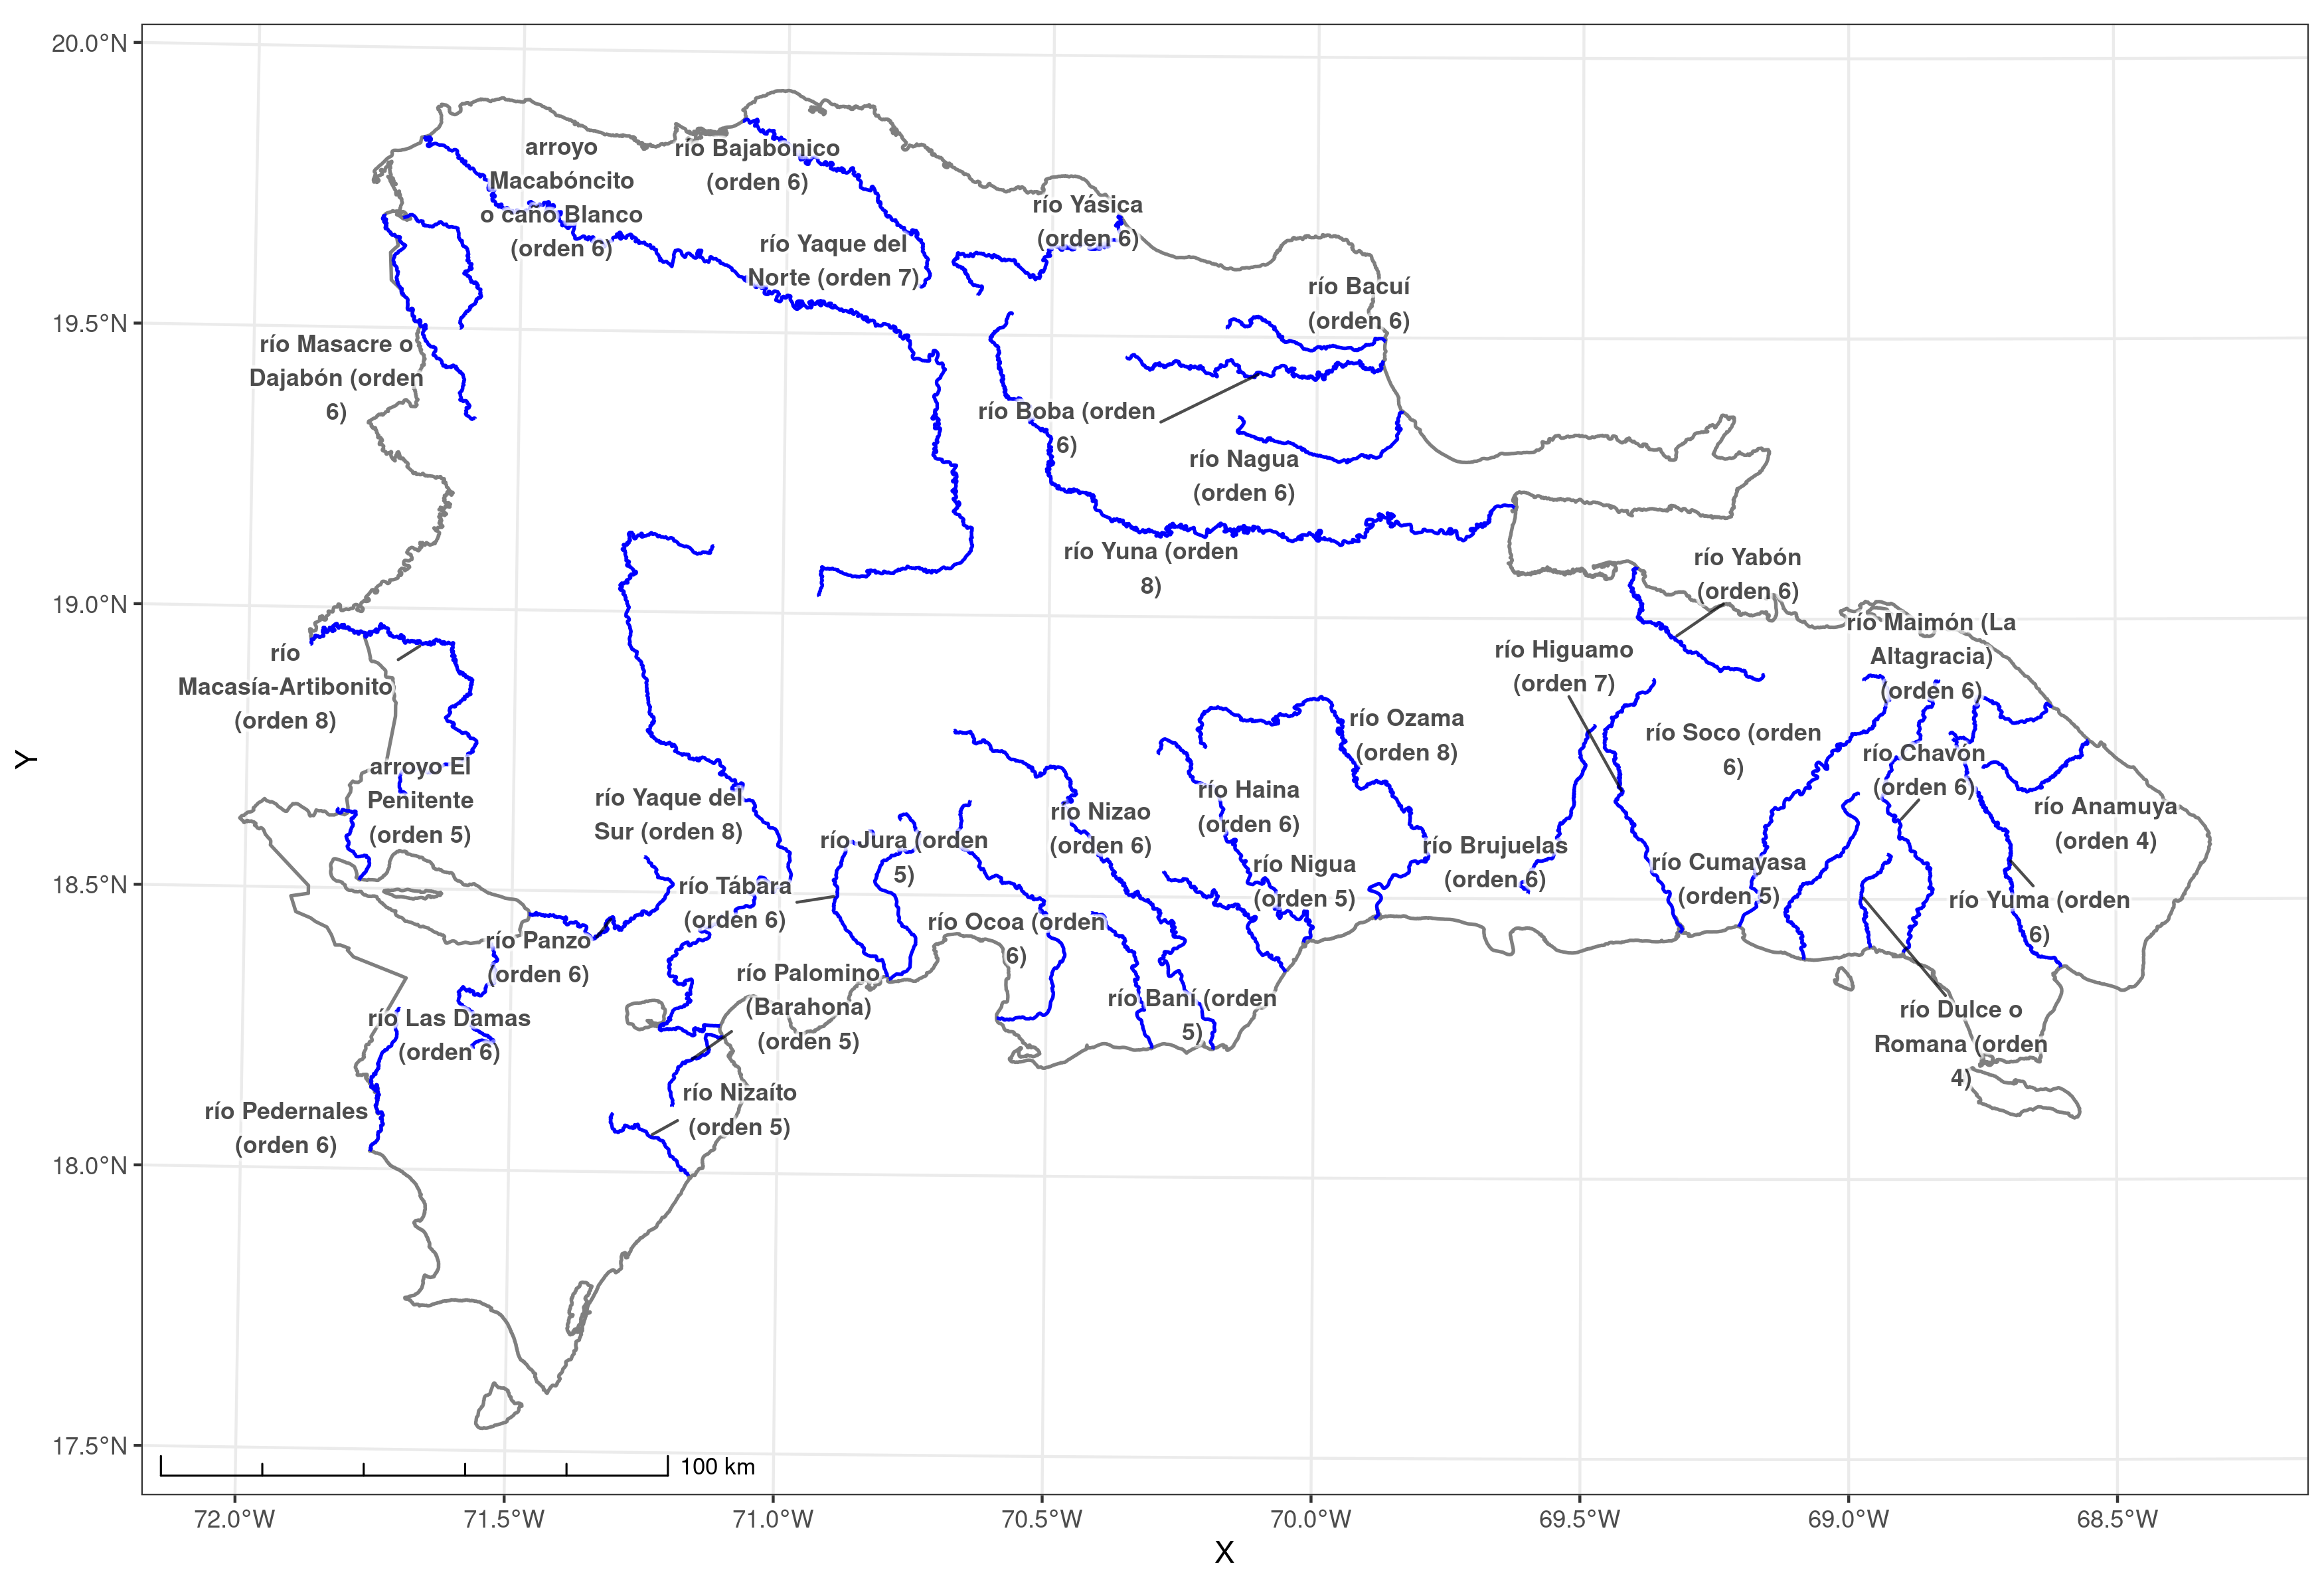
\includegraphics[width=1\linewidth]{figuras/cursos-mas-largos} 

}

\caption{Cursos más largos de 35 ríos seleccionados de la República Dominicana basados en orden de red y representatividad territorial. Se priorizaron ríos de orden seis o superior. En áreas del sur y sudoeste, se incluyeron ríos de orden cinco de notable longitud.}\label{fig:cursosmaslargos}
\end{figure}

\begin{table}[H]

\caption{\label{tab:tablacursosmaslargos}Longitud del curso más largo, y orden máximo, de 35 ríos seleccionados de República Dominicana, ordenados de mayor a menor longitud}
\centering
\begin{tabular}[t]{rlrr}
\toprule
Rango & Nombre & Longitud (km) & Orden máximo\\
\midrule
1 & río Yaque del Norte & 334.30 & 7\\
2 & río Yuna & 272.00 & 8\\
3 & río Yaque del Sur & 251.50 & 8\\
4 & río Nizao & 150.60 & 6\\
5 & río Ozama & 148.70 & 8\\
\addlinespace
6 & río Macasía-Artibonito & 128.10 & 8\\
7 & río Boba & 103.80 & 6\\
8 & río Soco & 94.38 & 6\\
9 & río Bajabonico & 92.16 & 6\\
10 & río Yásica & 88.50 & 6\\
\addlinespace
11 & río Haina & 87.74 & 6\\
12 & río Chavón & 86.63 & 6\\
13 & río Higuamo & 83.98 & 7\\
14 & río Ocoa & 83.35 & 6\\
15 & río Yuma & 81.45 & 6\\
\addlinespace
16 & río Masacre o Dajabón & 71.49 & 6\\
17 & río Panzo & 66.02 & 6\\
18 & río Yabón & 61.79 & 6\\
19 & río Nagua & 56.35 & 6\\
20 & río Cumayasa & 55.55 & 5\\
\addlinespace
21 & río Nigua & 55.11 & 5\\
22 & río Jura & 54.06 & 5\\
23 & río Bacuí & 51.50 & 6\\
24 & río Brujuelas & 50.99 & 6\\
25 & arroyo Macabóncito o caño Blanco & 48.78 & 6\\
\addlinespace
26 & río Las Damas & 48.41 & 6\\
27 & río Tábara & 46.21 & 6\\
28 & río Pedernales & 44.08 & 6\\
29 & río Baní & 43.26 & 5\\
30 & río Maimón (La Altagracia) & 42.15 & 6\\
\addlinespace
31 & río Anamuya & 41.45 & 4\\
32 & río Nizaíto & 29.57 & 5\\
33 & río Dulce o Romana & 27.66 & 4\\
34 & arroyo El Penitente & 26.77 & 5\\
35 & río Palomino (Barahona) & 25.56 & 5\\
\bottomrule
\end{tabular}
\end{table}

Por otro lado, tanto la pendiente promedio (celda a celda) como el
gradiente promedio (cabecera a desembocadura) muestran una disminución a
medida que aumenta el orden de red, siguiendo una típica relación
inversa exponencial (Figura~\ref{fig:variablesredesordenes}). Aunque se
trata de valores generalmente pequeños, pues se trata de métricas
tomadas por tramos o celda a celda, el rango de variación es sustancial.
La pendiente promedio para el primer orden es de 0.069~m/m ,
disminuyendo hasta 0.01~m/m en el octavo orden. En forma similar, el
gradiente promedio disminuye desde 0.064~m/m en el primer orden a
0.001~m/m en el octavo orden.

El último promedio analizado fue la diferencia de elevación. Esta
variable presenta un patrón distinto al de las anteriores, pues
incrementa su valor promedio desde el orden uno al cinco y, a partir de
este orden, se produce una inflexión y desciende hasta alcanzar el orden
ocho, aumentando al mismo tiempo su dispersión. En el orden uno, el
promedio de la diferencia de elevación fue de 37~m, alcanza un promedio
más alto de 127~m en el quinto orden de red, manteniéndose igualmente
alto en el seis (120~m). A partir de este orden, se produce un descenso
de los promedios, conjuntamente con un aumento de la dispersión, hasta
alcanzarse el valor de 79~m en el orden ocho.

También analizamos en detalle los cursos más largos de 35 ríos redes de
drenaje seleccionadas de República Dominicana. La selección de este
subconjunto la apoyamos en dos criterios: orden de red y
representatividad territorial. De manera preferente, incluimos cursos
fluviales de orden seis o superior. En áreas del sur y sudoeste del país
donde este orden no fue alcanzado, elegimos algunos ríos de orden cinco
de gran longitud. Este enfoque nos permitió obtener información valiosa
sobre los rasgos básicos de longitud y orden de red de los ríos más
largos y emblemáticos del país. Asimismo, al garantizar la
representatividad territorial, logramos abarcar cada una de las regiones
del país.

La Figura~\ref{fig:cursosmaslargos} muestra el trazado de los cursos más
largos de ríos seleccionados. Los más grandes y de mayor jerarquía, de
orden seis a ocho, se dividen en dos subgrupos distintos. El primer
subgrupo incluye cursos que siguen direcciones predominantes, como los
ubicados en el borde sudoriental de la cordillera Central (Haina, Nizao,
Nigua), aquellos que discurren por la vertiente meridional de la
cordillera Oriental (Higuamo, Soco, Chavón), y los localizados al este
de la cordillera Septentrional (Boba, Bacuí). El segundo subgrupo está
compuesto por cursos con trazados tortuosos, destacando especialmente
los ríos Ozama y Macasía-Artibonito, que alcanzaron un orden de red
elevado y presentan longitudes notables.

La Tabla~\ref{tab:tablacursosmaslargos} presenta los ríos seleccionados
en función de la longitud de su curso, ordenados de mayor a menor. El
río Yaque del Norte destaca con una longitud de 334~km y un orden máximo
de siete. Este río nace en el pico del Yaque en la cordillera Central y
desemboca en la bahía de Montecristi. Siguiendo en longitud, tenemos al
río Yuna con 272~km y un orden máximo de ocho, con curso más largo
extendiéndose por la cordillera Septentrional a través del río Licey,
tributario del río Camú. Notablemente, los ríos Yaque del Sur,
Macasía-Artibonito y Ozama tienen cursos más largos de 252, 128 y
149~km, respectivamente. Todos, incluido el Yuna, han alcanzado un orden
máximo de ocho, subrayando su relevancia en la red de drenaje a nivel
nacional. El Macasía-Artibonito es singular por lograr el orden máximo
siendo el sexto en longitud, mientras que el Nizao, siendo el cuarto más
largo con 151~km, alcanza solo el orden seis.

El resto de ríos en la tabla poseen cursos más largos de 100~km o menos,
y un orden de seis o inferior. Se dividen en dos categorías: entre 40 y
100~km, y aquellos de 40~km o menos. El primer grupo, de 40 a 100~km,
incluye 20 ríos, principalmente de orden seis, situados en las
cordilleras Oriental y Central que desembocan en el mar Caribe, así como
en la cordillera Septentrional que fluyen hacia el océano Atlántico.
Estos sistemas fluviales a menudo tienen cuencas extensas, y muchos se
originan o atraviesan regiones kársticas. Un caso destacado es el río
Higuamo, que, a pesar de ser el 13\(^\circ\) en longitud, tiene un orden
de siete. El segundo grupo, de menos de 40~km, comprende principalmente
ríos de los órdenes cinco y cuatro, ubicados en el sudoeste del país y
en zonas kársticas orientales.

Finalmente, determinamos la razón de bifurcación y la densidad de la red
de drenaje, tanto a nivel global como diferenciado por órdenes de red
(ver Tabla~\ref{tab:tablaredesordratios}). A escala global, la densidad
de drenaje se estableció en 2.11~km/km\(^2\). Por otro lado, al calcular
la razón de bifurcación, obtuvimos dos métricas distintas: 4.34
utilizando promedios, y 4.42 por medio de coeficientes de regresión.
Descomponiendo estos indicadores por órdenes de red, se identifica un
comportamiento distintivo en la densidad de drenaje: presenta un pico en
los órdenes iniciales, con 1.7~km/km\(^2\) en el primer orden, y exhibe
un descenso progresivo hasta alcanzar 0.0172~km/km\(^2\) en el octavo
orden. De manera similar, la razón de bifurcación refleja la esperada
disminución a medida que avanzamos en el orden, comenzando con 4.39 en
el primer orden y finalizando en 2.5 para el séptimo orden.

\begin{table}[H]

\caption{\label{tab:tablaredesordratios}Razones o cocientes de la red de drenaje}
\centering
\begin{tabular}[t]{rrr}
\toprule
Orden de red & Razón de bifurcación & Densidad de drenaje (km/km$^2$)\\
\midrule
1 & 4.39 & 1.70\\
2 & 4.61 & 0.84\\
3 & 4.71 & 0.43\\
4 & 4.73 & 0.23\\
5 & 4.35 & 0.12\\
\addlinespace
6 & 5.10 & 0.05\\
7 & 2.50 & 0.03\\
8 & 0.00 & 0.02\\
\bottomrule
\end{tabular}
\end{table}

\hypertarget{discusiuxf3n}{%
\section{Discusión}\label{discusiuxf3n}}

Elaboramos una representación detallada de cuencas hidrográficas y redes
de drenaje de República Dominicana, a partir del DEM proporcionado con
los productos ALOS PALSAR RTC. Con la aplicación de técnicas avanzadas
de hidrología computacional y análisis hortoniano (GRASS Development
Team, 2023; Horton, 1945; Jasiewicz y Metz, 2011; Strahler, 1957), no
sólo logramos mejorar la delimitación de cuencas y la extracción de
redes, sino que también caracterizamos los patrones fundamentales de la
hidrografía dominicana mediante estadísticos propios de la hidrología
computacional. Este avance es particularmente significativo en las áreas
montañosas, donde las fuentes hasta la fecha disponibles, mostraban una
red fragmentada o incompleta (INDRHI, 2012; Instituto Cartográfico
Militar (ICM), 1989; OpenStreetMap contributors, 2017; Secretaría de
Estado de Medio Ambiente y Recursos Naturales, 2004). Simultáneamente,
refinamos el DEM utilizado, priorizando el tallado de la red en zonas
llanas, minimizando el ruido y preservando los elementos morfológicos
esenciales para asegurar una precisión hidrológica máxima. Como parte de
nuestro apego a la transparencia y la accesibilidad en la investigación,
publicamos la base de datos generada en repositorio disponible al
público, sistematizamos un protocolo completamente reproducible y
desarrollamos una base de código abierto, posicionándola como una
herramienta esencial para futuros estudios en hidrología computacional.

La hidrología computacional y el análisis hortoniano de la hidrografía
dominicana, han tenido históricamente poco alcance debido a la limitada
disponibilidad de datos detallados y precisos. Previo a nuestro trabajo,
las fuentes más relevantes para estudios en la región se centraban
primordialmente en modelos digitales de elevación de resolución baja
(Jarvis et~al., 2008; NASA JPL, 2013; NASA LP DAAC, 2000; National
Aeronautics and Space Administration y United States Geological Survey,
2009), o en la cartografía topográfica base e investigaciones locales
(CIDIAT y INDRHI, 1992; INDRHI, 2012; Instituto Cartográfico Militar
(ICM), 1989; Secretaría de Estado de Medio Ambiente y Recursos
Naturales, 2004; SERCITEC y INDRHI, 2002). Estas publicaciones, aunque
fundamentales, carecían del nivel de detalle y la sistematización
necesaria para avanzar en la hidrología computacional y el análisis
hortoniano.

En este contexto de fuentes escasas, Martínez-Batlle (2019b) explora la
reorganización del drenaje en una subcuenca del río Ocoa durante el
Pleistoceno superior. A pesar de la relevancia de dicho trabajo, su
aplicabilidad a escala nacional, o incluso local, es limitada. En
contraposición, nuestro trabajo contribuye a rellenar este vacío, al
ofrecer una perspectiva detallada y amplia, primordial para efectuar
análisis tan profundos como el referido, pero a escala nacional. De esta
manera, allanamos el camino para investigaciones subsecuentes en el
dominio de la hidrología computacional.

La configuración y densidad de la red de drenaje generada por nosotros,
resalta claramente la influencia de la fisiografía y la diversidad
litológica de República Dominicana. La densidad de drenaje no es
aleatoria; está determinada por factores específicos como la
permeabilidad de las rocas y el suelo, la cantidad de precipitación, el
tamaño de la cuenca y sus características topográficas (Culler et~al.,
1961). En áreas caracterizadas por rocas impermeables, como margas y
esquistos, así como otras que al intemperizarse producen suelos de
textura fina, es típico encontrar densidades de drenaje y razones de
bifurcación elevadas (Anderson y Anderson, 2010; Horton, 1932; Horton,
1945; Strahler, 1957). Dichas condiciones son prevalentes en regiones
como el borde meridional de la cordillera Central, la cordillera
Septentrional, la cordillera Oriental y la sierra de Yamasa (Mollat
et~al., 2004; Pérez Estaún et~al., 2007), lo cual explica la jerarquía
alcanzada por ríos como el Yaque del Sur, Macasía-Artibonito, Ozama,
Yuna e Higuamo. Por otra parte, no podemos precisar si los valores
elevados de densidad de drenaje en subcuencas del río Yaque del Sur
ubicadas sobre margas y fangos, están asociados, conjuntamente con la
litología, a las mayores intensidades de precipitación comúnmente
observadas en esta zona del país, lo cual constituye una pregunta
abierta que requerirá futura investigación.

Nuestra red refleja la harmonización con los elementos
morfoestructurales del país, un sistema alternante de cordilleras y
amplios valles fluviales, dispuestos predominantemente en dirección
noroeste-sudeste. Esta disposición, moldeada por procesos geotectónicos
históricos y contemporáneos, guía la orientación de ríos prominentes
como el Yuna-Camú, Yaque del Norte y Yaque del Sur.

Asimismo, es innegable el impacto de los sistemas kársticos en la
organización de la red de drenaje. En este contexto, el karst de Los
Haitises es el más destacado, influyendo significativamente en la
estructuración de la red hidrográfica. Su característica de sumidero,
vinculada a la repetición monótona de dolinas con ponors que dirigen
flujos de agua hacia el endokarst, marca la ausencia de escorrentía
superficial jerarquizada entre la sierra de Yamasá y la cordillera
Oriental. Se observan influencias análogas, aunque de menor extensión,
en áreas del karst de plataforma de la llanura sudoriental, en la
cordillera Septentrional y en las sierras de Bahoruco y Neyba.

La Española es una isla originada a partir de una colisión derivada de
la convergencia oblicua entre la Placa Norteamericana y el arco-isla
Cretácico caribeño (Pérez Estaún et~al., 2007). Esto significa que se
trata de un país con un activo pasado geológico, donde los procesos de
reorganización del drenaje, resultado de la interacción entre litología,
tectónica y clima a lo largo del tiempo, han debido ser frecuentes. En
general, los ríos con trazado tortuoso, caracterizados por largos rodeos
entre su origen y desembocadura, a menudo son indicativos de una
reorganización del drenaje, como por ejemplo, captura fluvial (Bishop,
1995). Biogeográficamente, tales reorganizaciones tienen consecuencias
significativas, por lo que constituyen una línea de investigación muy
activa en varios sistemas fluviales del mundo (Barreto et~al., 2022;
Musher et~al., 2022). Nuestro análisis mostró varios casos de ríos cuyo
curso más largo sigue un trazado de amplio rodeo, con giros bruscos en
distintos puntos de sus respectivos recorridos, como por ejemplo los
ríos Yaque del Norte, Yaque del Sur y Ozama. Contrariamente, los ríos
con trazados rectilíneos podrían representar una fase evolutiva más
reciente de la isla, tal como ocurre en los ríos Nizao, Haina e Higuamo.
Estos patrones, en su conjunto, proporcionan una comprensión profunda de
cómo los procesos geomorfológicos, tectónicos, climáticos y biológicos
interactúan, modelando tanto el paisaje como la biodiversidad
dominicanos.

Nosotros pudimos comprobar la relación exponencial entre el orden de red
y distintas variables morfométricas de la estadística hortoniana, como
la razón de bifurcación, el área de cuencas y las longitudes de cursos,
entre otros (Horton, 1945). En cuanto a la razón de bifurcación, esta
sigue la regla del número de cursos o corrientes, que expresa la
relación existente entre el número de cursos de un orden dado y el orden
del curso en términos de una serie geométrica inversa. Los valores de
razón de bifurcación de ámbito nacional obtenidos por nosotros
(R\textsubscript{b}\textgreater~4.5), tanto mediante regresión como por
promedios, superan el valor comúnmente observado en este tipo de
estudios (3.5~\textless~R\textsubscript{b}~\textless~4). Este resultado
lo asociamos con el umbral de acumulación elegido por nosotros para
crear la red, de 8~ha, dado que se espera que a menor umbral de
acumulación, mayor razón de bifurcación. No obstante, dado que los
estudios realizados en el siglo pasado se basaban en extracciones de la
red a partir de mapas topográficos de escala 1:50,000, es esperable que
nuestra red, al ser más densa, alcance razones mayores.

Un aspecto destacable de nuestros resultados es la observación de que
los cursos o corrientes de órdenes 5 y 6 presentan, en promedio,
diferencias de elevación superiores en comparación con los otros órdenes
jerárquicos (1 a 4, y 7 a 8). Esta característica singular podría tener
su origen en la posición geomorfológica donde ocurren estos cursos,
preferentemente en zonas de transición, específicamente en enlaces con
piedemontes. Estas áreas suelen mostrar rasgos morfológicos donde el
drenaje experimenta una expansión vertical acusada, es decir, un cambio
de elevación del terreno de manera abrupta, sin que ello esté asociado
con un incremento en el orden de la red. Esta situación indica que en
estas zonas, las dinámicas geomorfológicas podrían estar favoreciendo un
relieve más pronunciado, sin necesariamente acompañarse de una mayor
complejidad en la estructura de drenaje. Nuestra interpretación resalta
la importancia de considerar no solo la jerarquía fluvial, sino también
la geomorfología local, al evaluar las características morfodinámicas de
una cuenca.

Nuestros resultados presentan limitaciones, inherentes a todo estudio,
que es preciso abordar en esta sección. En primer lugar, la precisión
posicional de la red varía significativamente dependiendo de la
geomorfología. Si bien es alta en sistemas montañosos no kársticos, se
modera en terrenos kársticos y disminuye en grandes llanuras y zonas de
desembocadura. Específicamente, en los relieves kársticos, enfrentamos
una alta incertidumbre dada la carencia de un catálogo exhaustivo de
depresiones con drenje endorreico, como las dolinas con ponors activos,
lo cual es esencial para definir la topología y jerarquización de la red
en dichos morfosistemas. Explicamos que, ante esta limitación,
desarrollamos un inventario propio de depresiones basado en el propio
DEM, el cual consideramos suficiente para nuestros fines, pero limitado
para aplicaciones más amplias sobre infiltración en el karst. También es
pertinente añadir que en zonas urbanas, áreas llanas, terrenos con
sistemas de riego y áreas de desembocadura (por ejemplo, en los ríos
Yaque del Sur y Yuna), la precisión de nuestra red puede verse muy
comprometida. Sin embargo, dado que nuestro objetivo se centra en la
generación sistemática de la hidrografía densa, con énfasis en las áreas
de montaña, el error posicional inherente no menoscaba la relevancia de
nuestros resultados.

En lo concerniente a las cuencas y redes de drenaje transfronterizas,
cabe señalar que las extraídas por nosotros se basan exclusivamente en
datos del territorio dominicano. Esto significa que el orden de red
máximo reportado para estas redes podría no ser representativo de su
orden verdadero. A pesar de esta restricción, nuestro análisis visual
preliminar sugiere que no compromete el objetivo central de nuestro
estudio. Es una línea que, en futuras investigaciones, será abordada de
forma integral, ofreciendo una visión más acabada de su morfometría.

Por último, en cuanto a las limitaciones esbozadas, para nosotros es
importante aclarar el alcance de nuestra singular propuesta nuestra
investigación. A diferencia de los enfoques convencionales que se
articulan en torno a preguntas e hipótesis, el nuestro se centra en la
generación y exposición de datos, así como en la producción de código
reproducible. Dado el énfasis en la construcción de la red hidrográfica
y la metodología rigurosa empleada, entendemos este trabajo como un
aporte esencialmente de carácter metodológico y para la producción de
datos, llenando un hueco en la bibliografía y generando una base de
datos y de código para futuros estudios sobre la hidrografía dominicana
y de otros territorios.

A partir de los resultados obtenidos y las observaciones registradas en
el presente estudio, es posible identificar diversas vías de
investigación futura que podrían enriquecer la caracterización de los
sistemas hídricos dominicanos realizada en el presente estudio. Nuestra
primera consideración se centra la precisión del modelo de elevación
utilizado. Entendemos que es crucial realizar una evaluación detallada
de la precisión para cuantificar el error posicional de la red
hidrográfica derivada, lo cual podría contribuir a potenciar la robustez
de resultados futuros. Una de propuesta de investigación relacionada,
consiste en colectar puntos mediante receptores GNSS en el terreno y
realizar, por distintos métodos, una revisión de precisión y
rectificación del modelo. Dado que las áreas llanas presentan mayores
retos, sería beneficioso refinar la hidrografía de estas zonas a medida
que se mejoren la precisión del modelo.

Por otra parte, los hallazgos del presente estudio pueden allanar el
camino para investigaciones que se adentren en fenómenos de
reorganización de drenaje, incorporando métricas más sofisticadas. Para
una mejor comprensión de los fenómenos geomorfológicos, sería oportuno
explorar el índice de concavidad, la hipsometría, el índice \(\chi\) y
las métricas de Gilbert, tal como se ha realizado para distintas
regiones en años recientes (Dal Pai et~al., 2023; Forte y Whipple, 2018;
Harkins et~al., 2007; Maneerat y Bürgmann, 2022; Pereira de Oliveira
et~al., 2023). Al mismo tiempo, un enfoque individualizado en las
cuencas, particularmente de aquellas de orden cuatro o superior, podría
proporcionar analíticas específicas sobre la dinámica y características
de dicho subconjunto.

Además, la morfometría de redes y cuencas debería recibir una atención
especial en futuros estudios. Este enfoque permitiría un entendimiento
más profundo de las propiedades y el comportamiento de la red fluvial y
de las cuencas en general. Paralelamente, sería provechoso realizar
análisis hortonianos más exhaustivos, que aborden la estructura,
jerarquía y distribución espacial de las redes de drenaje según rasgos
comunes que ayuden a clasificar mejor la hidrografía dominicana.

Por último, resulta esencial estudiar la relación y patrones de
asociación entre diferentes variables de las cuencas (e.g.~densidad de
drenaje), y a su vez confrontarlas con características del medio físico
como la elevación, pendiente, litología, geomorfología y,
particulamente, con el clima. Una dirección prometedora en la
investigación podría explorar si las densidades de drenaje más altas en
las cuencas del borde meridional de la cordillera Central, como en el
Cinturón de Peralta, están vinculadas tanto a la litología como al
clima. Herramientas como \texttt{r.basin} (de GRASS GIS) podrían
facilitar este proceso, revelando interacciones y correlaciones hasta
ahora no identificadas.

Finalmente, sobre la relevancia de nuestro estudio, los resultados
obtenidos representan un hito en la investigación hidrológica de la
República Dominicana, siendo la primera vez que se aborda la hidrología
computacional a nivel nacional de manera coherente y sistemática. Con la
caracterización realizada, hemos generado una red hidrográfica densa que
sirve como base apropiada para realizar comparaciones sistemáticas, así
como numerosos estudios y aplicaciones prácticas.

Nuestros resultados tienen potencial para aplicaciones en diversos
ámbitos, desde el diseño de estrategias de conservación de cuencas y la
modelización hidrológica en zonas altas y medias, hasta la contribución
en estudios de riesgos y en el diseño de redes hidrométricas. Además, la
red generada proporciona una base idónea para futuras investigaciones
sobre la biodiversidad y su conservación, facilitando el diseño de
muestreos de flora y fauna acuática en sistemas fluviales de montaña
media y alta.

Por otro lado, por nuestro compromiso con la transparencia y la
educación, hemos generado una base de código informático conjuntamente
con el protocolo seguido, que no sólo garantizan la replicabilidad del
estudio sino que también se ofrece un valioso recurso didáctico.
Estudiantes, tanto de grado como de posgrado, y profesionales
interesados en la hidrología, encontrarán en nuestra investigación una
guía detallada para aplicar métodos similares a otras fuentes de
elevación.

En conclusión, nuestro estudio abre un camino innovador en la
comprensión de la hidrografía de República Dominicana, fusionando
tecnologías y metodologías computacionales con un análisis sistemático a
nivel nacional. La caracterización detallada y sistemática de la
hidrografía ha desvelado la intrincada red fluvial del país, ofreciendo
una herramienta invaluable para aplicaciones prácticas y científicas,
desde la conservación de cuencas hasta la modelización hidrológica. Nos
hemos apoyado en el rigor metodológico y en las fuentes de datos de
mayor detalle disponibles públicamente, para generar un producto que,
aunque reconocemos que es mejorable, enriquece nuestra comprensión de la
geografía física dominicana y sienta un precedente para investigaciones
futuras, estableciendo un marco de referencia que puede ser replicado o
adaptado en otros contextos y regiones. La combinación de datos,
protocolos y análisis que hemos presentado en este trabajo, junto con la
relevancia de su contenido, evidencia la trascendencia de la
investigación.

\hypertarget{declaraciuxf3n-de-conflicto-de-intereses}{%
\section*{Declaración de conflicto de
intereses}\label{declaraciuxf3n-de-conflicto-de-intereses}}
\addcontentsline{toc}{section}{Declaración de conflicto de intereses}

El autor y la autora declaran que no tienen ningún conflicto de interés
con el contenido de este artículo.

\hypertarget{disponibilidad-de-datos-scripts-y-cuxf3digo}{%
\section*{Disponibilidad de datos, scripts y
código}\label{disponibilidad-de-datos-scripts-y-cuxf3digo}}
\addcontentsline{toc}{section}{Disponibilidad de datos, scripts y
código}

Los datos que respaldan los hallazgos de este estudio están disponibles
abiertamente en Zenodo en \url{https://doi.org/10.5281/zenodo.8146391}
(Martínez-Batlle y Izzo-Gioiosa, 2023). Los scripts utilizados para la
curación de datos, análisis y visualización están disponibles en esta
sección, así como en el repositorio de GitHub en
\url{https://github.com/geofis/red-hidrografica-densa-rd} y en Zenodo en
\url{} (\textbf{RELLENAR?}).

\newpage

\hypertarget{infosupl}{%
\section*{Información suplementaria}\label{infosupl}}
\addcontentsline{toc}{section}{Información suplementaria}

\beginsupplement

\hypertarget{suplemento-metodoluxf3gico-para-la-subsecciuxf3n-obtenciuxf3n-y-preprocesamiento-del-dem}{%
\subsection*{Suplemento metodológico para la subsección ``Obtención y
Preprocesamiento del
DEM''}\label{suplemento-metodoluxf3gico-para-la-subsecciuxf3n-obtenciuxf3n-y-preprocesamiento-del-dem}}
\addcontentsline{toc}{subsection}{Suplemento metodológico para la
subsección ``Obtención y Preprocesamiento del DEM''}

Los siguientes bloques de código cargan los paquetes de uso común a lo
largo de este cuaderno, así como funciones creadas por nosotros para
eficientizar las tareas de limpieza y representación de datos y mapas.
Igualmente, aprovechamos este bloque de código para declarar la ruta del
directorio donde se alojan los archivos fuente, la cual reaprovechamos
en distintas partes del código.

\begin{Shaded}
\begin{Highlighting}[]
\NormalTok{conflicted}\SpecialCharTok{::}\FunctionTok{conflict\_prefer}\NormalTok{(}\StringTok{"select"}\NormalTok{, }\StringTok{"dplyr"}\NormalTok{)}
\NormalTok{conflicted}\SpecialCharTok{::}\FunctionTok{conflict\_prefer}\NormalTok{(}\StringTok{"filter"}\NormalTok{, }\StringTok{"dplyr"}\NormalTok{)}
\NormalTok{conflicted}\SpecialCharTok{::}\FunctionTok{conflict\_prefer}\NormalTok{(}\StringTok{"distance"}\NormalTok{, }\StringTok{"raster"}\NormalTok{)}
\NormalTok{conflicted}\SpecialCharTok{::}\FunctionTok{conflict\_prefer}\NormalTok{(}\StringTok{"alpha"}\NormalTok{, }\StringTok{"ggplot2"}\NormalTok{)}
\NormalTok{conflicted}\SpecialCharTok{::}\FunctionTok{conflict\_prefer}\NormalTok{(}\StringTok{"rescale"}\NormalTok{, }\StringTok{"scales"}\NormalTok{)}
\FunctionTok{library}\NormalTok{(psych)}
\FunctionTok{library}\NormalTok{(raster)}
\FunctionTok{library}\NormalTok{(sf)}
\FunctionTok{library}\NormalTok{(kableExtra)}
\FunctionTok{library}\NormalTok{(tidyverse)}
\FunctionTok{library}\NormalTok{(gdalUtilities)}
\FunctionTok{library}\NormalTok{(e1071)}
\FunctionTok{library}\NormalTok{(scales)}
\FunctionTok{library}\NormalTok{(tmap)}
\FunctionTok{library}\NormalTok{(janitor)}
\FunctionTok{library}\NormalTok{(ggrepel)}
\FunctionTok{library}\NormalTok{(ggsflabel)}
\FunctionTok{library}\NormalTok{(spanish)}
\FunctionTok{source}\NormalTok{(}\StringTok{\textquotesingle{}R/funciones.R\textquotesingle{}}\NormalTok{)}
\FunctionTok{rm}\NormalTok{(}\AttributeTok{list =} \FunctionTok{grep}\NormalTok{(}\StringTok{\textquotesingle{}RR\_*\textquotesingle{}}\NormalTok{, }\FunctionTok{ls}\NormalTok{(), }\AttributeTok{value =}\NormalTok{ T)) }\CommentTok{\#Borrar resúmenes sesión anterior}
\NormalTok{dem\_proc\_dir }\OtherTok{\textless{}{-}} \StringTok{\textquotesingle{}estadisticos\textquotesingle{}}
\NormalTok{figuras }\OtherTok{\textless{}{-}} \StringTok{\textquotesingle{}figuras\textquotesingle{}}
\NormalTok{umbral\_espurias }\OtherTok{\textless{}{-}} \DecValTok{4000} \CommentTok{\#Umbral por debajo del cual se considera una cuenca como espuria}
\end{Highlighting}
\end{Shaded}

Descargamos 42 escenas ALOS PALSAR RTC, específicamente los \emph{Hi-Res
Terrain Corrected}, desde el Centro de Archivo Activo Distribuido (DAAC)
del \href{https://asf.alaska.edu/}{Alaska Satellite Facility (ASF)} (ASF
DAAC, 2014), para posteriormente depurarlas y seleccionar las más
idóneas para unirlas en un mosaico creado como ráster virtual. La
descarga la realizamos por lotes, usando un \emph{script} de Python
provisto por el propio ASF.

\begin{Shaded}
\begin{Highlighting}[]
\NormalTok{python download}\OperatorTok{{-}}\BuiltInTok{all}\OperatorTok{{-}}\DecValTok{2023}\OperatorTok{{-}}\DecValTok{0}\ErrorTok{4}\OperatorTok{{-}}\DecValTok{20\_00}\OperatorTok{{-}}\DecValTok{30}\OperatorTok{{-}}\FloatTok{00.}\ErrorTok{py}
\end{Highlighting}
\end{Shaded}

\begin{quote}
Al momento de realizarse esta investigación, la tendencia en el análisis
de datos geoespaciales apuntaba hacia enfoques basados en la nube, como
Google Earth Engine y Microsoft Planetary Computer. Nosotros usamos
regulamente estas plataformas en nuestras investigaciones, pero ciertos
algoritmos esenciales para el análisis hidrológico aún no se encuentran
disponibles en estos servicios. Por esta razón, nos vimos en la
necesidad de utilizar nuestros propios equipos informáticos (Intel(R)
Core(TM) i7-7700K CPU @ 4.20GHz, 64 GB de memoria RAM, unidad de estado
sólido NVMe, corriendo bajo Ubuntu 20.04) y, aunque conseguimos
paralelizar ciertos procesos, la mayoría de los algoritmos de
hidrolología computacional no utilizan eficientemente los múltiples
núcleos de los procesadores, resultando en una subutilización de la
capacidad de memoria y en procesamientos más lentos que los que
comúnmente se conseguirían en la nube.
\end{quote}

Identificamos las escenas necesarias para cubrir íntegramente la
República Dominicana, usando una búsqueda geográfica mediante polígono
delimitador en ASF. Dado que la misión del ALOS-PALSAR ofrece escenas de
distintas fechas para una misma área, las descargamos todas y
posteriormente excluimos del análisis las redundantes, conservando
siempre la más reciente. Utilizando el índice de huellas de escenas,
escribimos un pequeño programa para seleccionar las más recientes allí
donde hubiese redundancia. Con esto construimos un índice de DEM para
guiarnos durante la construcción del ráster virtual.

\begin{Shaded}
\begin{Highlighting}[]
\NormalTok{ind\_orig }\OtherTok{\textless{}{-}} \FunctionTok{invisible}\NormalTok{(}
  \FunctionTok{st\_read}\NormalTok{(}\StringTok{\textquotesingle{}alos{-}palsar{-}dem{-}rd/asf{-}datapool{-}results{-}2023{-}04{-}19\_08{-}31{-}26.geojson\textquotesingle{}}\NormalTok{,}
          \AttributeTok{quiet =}\NormalTok{ T)) }\SpecialCharTok{\%\textgreater{}\%} 
   \FunctionTok{rownames\_to\_column}\NormalTok{(}\StringTok{\textquotesingle{}fila\textquotesingle{}}\NormalTok{) }\SpecialCharTok{\%\textgreater{}\%} \FunctionTok{mutate}\NormalTok{(}\AttributeTok{fila =} \FunctionTok{as.integer}\NormalTok{(fila))}
\NormalTok{distancias }\OtherTok{\textless{}{-}}\NormalTok{ ind\_orig }\SpecialCharTok{\%\textgreater{}\%} \FunctionTok{st\_centroid}\NormalTok{() }\SpecialCharTok{\%\textgreater{}\%} \FunctionTok{st\_distance}\NormalTok{() }\SpecialCharTok{\%\textgreater{}\%}\NormalTok{ units}\SpecialCharTok{::}\FunctionTok{drop\_units}\NormalTok{()}
\NormalTok{distancias[}\FunctionTok{upper.tri}\NormalTok{(distancias, }\AttributeTok{diag =}\NormalTok{ T)] }\OtherTok{\textless{}{-}} \ConstantTok{NA}
\NormalTok{indices }\OtherTok{\textless{}{-}} \FunctionTok{which}\NormalTok{(distancias }\SpecialCharTok{\textless{}} \DecValTok{1000}\NormalTok{, }\AttributeTok{arr.ind =} \ConstantTok{TRUE}\NormalTok{)}
\NormalTok{duplicados }\OtherTok{\textless{}{-}} \FunctionTok{as.data.frame}\NormalTok{(indices) }\SpecialCharTok{\%\textgreater{}\%} 
  \FunctionTok{mutate}\NormalTok{(}\AttributeTok{dup\_id =} \DecValTok{1}\SpecialCharTok{:}\FunctionTok{nrow}\NormalTok{(indices)) }\SpecialCharTok{\%\textgreater{}\%} 
  \FunctionTok{pivot\_longer}\NormalTok{(}\SpecialCharTok{{-}}\NormalTok{dup\_id, }\AttributeTok{names\_to =} \StringTok{\textquotesingle{}tipo\textquotesingle{}}\NormalTok{, }\AttributeTok{values\_to =} \StringTok{\textquotesingle{}fila\textquotesingle{}}\NormalTok{) }\SpecialCharTok{\%\textgreater{}\%} 
  \FunctionTok{select}\NormalTok{(}\SpecialCharTok{{-}}\NormalTok{tipo)}
\NormalTok{seleccionados }\OtherTok{\textless{}{-}}\NormalTok{ duplicados }\SpecialCharTok{\%\textgreater{}\%}
  \FunctionTok{inner\_join}\NormalTok{(ind\_orig }\SpecialCharTok{\%\textgreater{}\%} \FunctionTok{select}\NormalTok{(fila, startTime) }\SpecialCharTok{\%\textgreater{}\%}\NormalTok{ st\_drop\_geometry) }\SpecialCharTok{\%\textgreater{}\%} 
  \FunctionTok{group\_by}\NormalTok{(dup\_id) }\SpecialCharTok{\%\textgreater{}\%} \FunctionTok{filter}\NormalTok{(startTime }\SpecialCharTok{==} \FunctionTok{max}\NormalTok{(startTime)) }\SpecialCharTok{\%\textgreater{}\%} \FunctionTok{pull}\NormalTok{(fila)}
\NormalTok{ind\_orig\_sel }\OtherTok{\textless{}{-}}\NormalTok{ ind\_orig }\SpecialCharTok{\%\textgreater{}\%}
  \FunctionTok{filter}\NormalTok{(}\SpecialCharTok{!}\NormalTok{fila }\SpecialCharTok{\%in\%}\NormalTok{ duplicados}\SpecialCharTok{$}\NormalTok{fila }\SpecialCharTok{|}\NormalTok{ fila }\SpecialCharTok{\%in\%}\NormalTok{ seleccionados) }\SpecialCharTok{\%\textgreater{}\%} 
  \FunctionTok{filter}\NormalTok{(centerLon }\SpecialCharTok{\textless{}} \SpecialCharTok{{-}}\FloatTok{72.1821}\NormalTok{)}
\end{Highlighting}
\end{Shaded}

\begin{Shaded}
\begin{Highlighting}[]
\NormalTok{ind\_orig\_sel }\SpecialCharTok{\%\textgreater{}\%} \FunctionTok{select}\NormalTok{(sceneName, startTime) }\SpecialCharTok{\%\textgreater{}\%} \FunctionTok{st\_drop\_geometry}\NormalTok{() }\SpecialCharTok{\%\textgreater{}\%}
  \FunctionTok{estilo\_kable}\NormalTok{(}\AttributeTok{titulo =} \FunctionTok{paste}\NormalTok{(}\StringTok{\textquotesingle{}Escenas ALOS{-}PALSAR usadas para generar un DEM de 12.5 m de}
\StringTok{                        resolución espacial de República Dominicana\textquotesingle{}}\NormalTok{))}
\end{Highlighting}
\end{Shaded}

\begin{table}[H]

\caption{\label{tab:tablaindice}Escenas ALOS-PALSAR usadas para generar un DEM de 12.5 m de
                        resolución espacial de República Dominicana}
\centering
\begin{tabu} to \linewidth {>{\raggedright}X>{\raggedright}X}
\toprule
sceneName & startTime\\
\midrule
ALPSRP253240380 & 2010-10-25 23:18:16\\
ALPSRP253240370 & 2010-10-25 23:18:08\\
ALPSRP253240360 & 2010-10-25 23:17:59\\
ALPSRP253240350 & 2010-10-25 23:17:51\\
ALPSRP252510370 & 2010-10-20 23:11:46\\
\addlinespace
ALPSRP252510360 & 2010-10-20 23:11:38\\
ALPSRP252510350 & 2010-10-20 23:11:30\\
ALPSRP251490380 & 2010-10-13 23:22:45\\
ALPSRP251490370 & 2010-10-13 23:22:36\\
ALPSRP251490360 & 2010-10-13 23:22:28\\
\addlinespace
ALPSRP251490350 & 2010-10-13 23:22:20\\
ALPSRP251490340 & 2010-10-13 23:22:12\\
ALPSRP250760380 & 2010-10-08 23:16:23\\
ALPSRP250760370 & 2010-10-08 23:16:15\\
ALPSRP250760360 & 2010-10-08 23:16:06\\
\addlinespace
ALPSRP250760350 & 2010-10-08 23:15:58\\
ALPSRP250030360 & 2010-10-03 23:09:44\\
ALPSRP250030350 & 2010-10-03 23:09:36\\
ALPSRP248280370 & 2010-09-21 23:14:21\\
ALPSRP248280360 & 2010-09-21 23:14:13\\
\addlinespace
ALPSRP248280350 & 2010-09-21 23:14:05\\
ALPSRP247260360 & 2010-09-14 23:25:03\\
ALPSRP247260350 & 2010-09-14 23:24:55\\
ALPSRP247260340 & 2010-09-14 23:24:47\\
ALPSRP242300380 & 2010-08-11 23:21:28\\
\addlinespace
ALPSRP242300370 & 2010-08-11 23:21:19\\
ALPSRP242300360 & 2010-08-11 23:21:11\\
ALPSRP242300350 & 2010-08-11 23:21:03\\
\bottomrule
\end{tabu}
\end{table}

En total, para cubrir el territorio de República Dominicana, necesitamos
28 de escenas únicas ALOS PALSAR RTC. Señalamos en este punto un detalle
relevante para el análisis hidrológico. Las escenas correspondientes a
la porción haitiana del río Artibonito, no las procesamos en este
estudio, a efectos de agilizar la producción de resultados. No obstante,
dicha tarea nos quedó pendiente para futuras investigaciones.

\begin{Shaded}
\begin{Highlighting}[]
\NormalTok{ind\_orig\_sel\_m }\OtherTok{\textless{}{-}}\NormalTok{ ind\_orig\_sel }\SpecialCharTok{\%\textgreater{}\%}
\NormalTok{  ggplot }\SpecialCharTok{+}
  \FunctionTok{geom\_sf}\NormalTok{(}\AttributeTok{alpha =} \FloatTok{0.6}\NormalTok{, }\AttributeTok{fill =} \StringTok{\textquotesingle{}grey90\textquotesingle{}}\NormalTok{, }\AttributeTok{color =} \StringTok{\textquotesingle{}grey20\textquotesingle{}}\NormalTok{, }\AttributeTok{size =} \FloatTok{0.5}\NormalTok{) }\SpecialCharTok{+}
  \FunctionTok{geom\_sf}\NormalTok{(}\AttributeTok{data =}\NormalTok{ pais, }\AttributeTok{fill =} \StringTok{\textquotesingle{}transparent\textquotesingle{}}\NormalTok{, }\AttributeTok{color =} \StringTok{\textquotesingle{}black\textquotesingle{}}\NormalTok{) }\SpecialCharTok{+}
\NormalTok{  ggplot2}\SpecialCharTok{::}\FunctionTok{geom\_sf\_label}\NormalTok{(}\FunctionTok{aes}\NormalTok{(}\AttributeTok{label =}\NormalTok{ sceneName), }\AttributeTok{color =} \StringTok{\textquotesingle{}red\textquotesingle{}}\NormalTok{, }\AttributeTok{size =} \FloatTok{1.5}\NormalTok{,}
                \AttributeTok{label.padding =} \FunctionTok{unit}\NormalTok{(}\FloatTok{0.1}\NormalTok{, }\StringTok{"lines"}\NormalTok{), }\AttributeTok{alpha =} \FloatTok{0.9}\NormalTok{) }\SpecialCharTok{+}
  \FunctionTok{theme\_bw}\NormalTok{() }\SpecialCharTok{+} 
  \FunctionTok{theme}\NormalTok{(}\AttributeTok{plot.title =} \FunctionTok{element\_text}\NormalTok{(}\AttributeTok{size =} \DecValTok{11}\NormalTok{)) }\SpecialCharTok{+}
\NormalTok{  ggspatial}\SpecialCharTok{::}\FunctionTok{annotation\_scale}\NormalTok{(}\AttributeTok{style =} \StringTok{\textquotesingle{}ticks\textquotesingle{}}\NormalTok{)}
\end{Highlighting}
\end{Shaded}

Usando como referencia el índice de escenas seleccionadas, extrajimos
los DEM correspondientes, incluidos en formato GTiff dentro de los
archivos comprimidos (\texttt{.zip}). Este formato es proporcionado por
el Alaska Satellite Facility para minimizar el uso del ancho de banda
durante las descargas, lo que resulta beneficioso para el rendimiento de
sus servidores. A pesar de estar comprimidos, la descompresión de estos
archivos no supone un proceso largo o laborioso.

\begin{Shaded}
\begin{Highlighting}[]
\NormalTok{zip\_path }\OtherTok{\textless{}{-}} \StringTok{\textquotesingle{}alos{-}palsar{-}dem{-}rd/\textquotesingle{}}
\FunctionTok{sapply}\NormalTok{(ind\_orig\_sel}\SpecialCharTok{$}\NormalTok{fileName, }
       \ControlFlowTok{function}\NormalTok{(x)}
         \FunctionTok{unzip}\NormalTok{(}
           \AttributeTok{zipfile =} \FunctionTok{paste0}\NormalTok{(zip\_path, x),}
           \AttributeTok{exdir =} \FunctionTok{paste0}\NormalTok{(zip\_path, }\StringTok{\textquotesingle{}dem\textquotesingle{}}\NormalTok{), }\AttributeTok{junkpaths =}\NormalTok{ T,}
           \AttributeTok{files =} \FunctionTok{paste0}\NormalTok{(}\FunctionTok{gsub}\NormalTok{(}\StringTok{\textquotesingle{}.zip\textquotesingle{}}\NormalTok{, }\StringTok{\textquotesingle{}\textquotesingle{}}\NormalTok{, x), }\StringTok{\textquotesingle{}/\textquotesingle{}}\NormalTok{, }\FunctionTok{gsub}\NormalTok{(}\StringTok{\textquotesingle{}zip\textquotesingle{}}\NormalTok{, }\StringTok{\textquotesingle{}dem.tif\textquotesingle{}}\NormalTok{, x)))}
\NormalTok{       )}
\end{Highlighting}
\end{Shaded}

Todos los DEM fueron proporcionados por ASF en el sistema de coordenadas
Universal Transversal de Mercator (UTM). Sin embargo, los situados al
oeste fueron suministrados en el huso 18N. Identificamos estos DEM y los
transformamos al huso 19N, que es el que corresponde a nuestra área, con
el objetivo de generar un producto continuo. Para realizar esta
transformación, empleamos la herramienta \texttt{gdalwarp} de la
biblioteca GDAL (GDAL/OGR contributors, 2022).

\begin{Shaded}
\begin{Highlighting}[]
\NormalTok{dems\_orig\_path }\OtherTok{\textless{}{-}} \FunctionTok{list.files}\NormalTok{(}\AttributeTok{path =} \StringTok{\textquotesingle{}alos{-}palsar{-}dem{-}rd/dem\textquotesingle{}}\NormalTok{,}
                             \AttributeTok{pattern =} \StringTok{\textquotesingle{}*dem.tif\textquotesingle{}}\NormalTok{, }\AttributeTok{full.names =}\NormalTok{ T)}
\NormalTok{crs\_18n }\OtherTok{\textless{}{-}} \FunctionTok{names}\NormalTok{(}\FunctionTok{which}\NormalTok{(}\FunctionTok{sapply}\NormalTok{(dems\_orig\_path, }\ControlFlowTok{function}\NormalTok{(x)\{}
\NormalTok{  crs\_x }\OtherTok{\textless{}{-}} \FunctionTok{gdal\_crs}\NormalTok{(x)}
\NormalTok{  is\_z18 }\OtherTok{\textless{}{-}} \FunctionTok{grepl}\NormalTok{(}\StringTok{\textquotesingle{}zone 18N\textquotesingle{}}\NormalTok{, crs\_x[[}\StringTok{\textquotesingle{}wkt\textquotesingle{}}\NormalTok{]])}
\NormalTok{\})))}
\FunctionTok{sapply}\NormalTok{(crs\_18n, }\ControlFlowTok{function}\NormalTok{(x) }\FunctionTok{file.rename}\NormalTok{(}\AttributeTok{from =}\NormalTok{ x, }\AttributeTok{to =} \FunctionTok{gsub}\NormalTok{(}\StringTok{\textquotesingle{}.tif\textquotesingle{}}\NormalTok{, }\StringTok{\textquotesingle{}\_z18n.tif\textquotesingle{}}\NormalTok{, x)))}
\NormalTok{crs\_18n\_ren }\OtherTok{\textless{}{-}} \FunctionTok{list.files}\NormalTok{(}\AttributeTok{path =} \StringTok{\textquotesingle{}alos{-}palsar{-}dem{-}rd/dem\textquotesingle{}}\NormalTok{,}
                          \AttributeTok{pattern =} \StringTok{\textquotesingle{}z18n.tif\textquotesingle{}}\NormalTok{, }\AttributeTok{full.names =}\NormalTok{ T)}
\FunctionTok{sapply}\NormalTok{(crs\_18n\_ren, }\ControlFlowTok{function}\NormalTok{(x)\{}
  \FunctionTok{gdalwarp}\NormalTok{(}
  \AttributeTok{srcfile =}\NormalTok{ x,}
  \AttributeTok{dstfile =} \FunctionTok{gsub}\NormalTok{(}\StringTok{\textquotesingle{}\_z18n.tif\textquotesingle{}}\NormalTok{, }\StringTok{\textquotesingle{}.tif\textquotesingle{}}\NormalTok{, x), }
  \AttributeTok{t\_srs =} \StringTok{\textquotesingle{}EPSG:32619\textquotesingle{}}\NormalTok{, }\AttributeTok{overwrite =}\NormalTok{ T)\})}
\end{Highlighting}
\end{Shaded}

A efectos de eficientizar la manipulación del DEM, creamos un ráster
virtual (VRT) usando la herramienta \texttt{gdalbuildvrt} de la
biblioteca GDAL. Un ráster virtual es básicamente la abstracción de una
imagen que se genera \emph{on the fly}, creado a partir de un índice de
tamaño pequeño, en formato XML, que apunta a los archivos originales sin
moverlos ni alterarlos. Tienen las mismas prestaciones que las imágenes
guardadas permanentes guardadas en disco, por lo que con un ráster
virtual podemos visualizar un mosaico continuo o realizar análisis
intermedios, o evaluar un producto antes de crearlo de forma definitiva.
Se trata de un formato muy eficiente que ayuda a ahorrar espacio en
disco.

\begin{Shaded}
\begin{Highlighting}[]
\FunctionTok{gdalbuildvrt}\NormalTok{(}\AttributeTok{gdalfile =}\NormalTok{ dems\_orig\_path,}
             \AttributeTok{output.vrt =} \FunctionTok{paste0}\NormalTok{(}\FunctionTok{paste0}\NormalTok{(zip\_path, }\StringTok{\textquotesingle{}dem\textquotesingle{}}\NormalTok{), }\StringTok{\textquotesingle{}/dem\_seamless.vrt\textquotesingle{}}\NormalTok{),}
             \AttributeTok{resolution =} \StringTok{\textquotesingle{}highest\textquotesingle{}}\NormalTok{, }\AttributeTok{r =} \StringTok{\textquotesingle{}average\textquotesingle{}}\NormalTok{)}
\end{Highlighting}
\end{Shaded}

Posterioremente, creamos la base de datos y localización de GRASS GIS
usando como fuente de extensión y resolución el ráster virtual (GRASS
Development Team, 2023). Decidimos usar GRASS GIS a partir de este punto
para prácticamente todas las tareas de análisis geoespacial e
hidrológico, pues se trata de un software bastante eficiente en muchos
de sus complementos y algoritmos de serie (e.g.~rellenado de nulos). Sin
embargo, en pasos posteriores, alternamos el flujo de procesamiento con
otras herramientas, como WhiteboxTools (Lindsay, 2018). En todo caso,
nuestro criterio fue siempre aprovechar al máximo los recursos de
hardware y software disponibles para obtener los productos requeridos en
el menor tiempo posible.

\begin{Shaded}
\begin{Highlighting}[]
\CommentTok{\# Usando Bash, desde la ruta ./alos{-}palsar{-}dem{-}rd/dem}
\ExtensionTok{grass} \AttributeTok{{-}{-}text} \AttributeTok{{-}c}\NormalTok{ dem\_seamless.vrt ./grassdata}
\CommentTok{\# Para abrir luego de cerrada: grass grassdata/PERMANENT/}
\end{Highlighting}
\end{Shaded}

Luego creamos una máscara de país en QGIS (QGIS Development Team, 2021),
superponiendo el límite oficial obtenido desde la página de la
\href{https://www.one.gob.do/}{Oficina Nacional de Estadística (ONE)}, y
combinándolo con otras fuentes disponibles en línea, como
\href{https://gadm.org/}{GADM},
\href{https://data.humdata.org/dataset/cod-ab-dom}{Humanitarian Data
Exchange (OCHA)} y \href{https://www.openstreetmap.org}{OpenStreetMap}
(GADM, 2022; OCHA, 2022; Oficina Nacional de Estadística (ONE), 2018;
OpenStreetMap contributors, 2017). De la máscara, eliminamos las
superficies de máximas de lagos y lagunas no artificiales, pues nos
interesa procesar las cuencas endorreicas que drenan hacia ellos. No
obstante, los embalses no los incluimos en dicha superficie, dado que
necesitamos construir la jerarquía de red ignorando su presencia, es
decir, asumiendo como continuos todos los cursos fluviales. Sobre esta
máscara, creamos un área de influencia, para recortar el DEM con un
cierto ``acolchado'' que nos permitiera análizar sin dificultades las
áreas costeras y de frontera. La creación de esta máscara fue el único
paso que realizamos de forma semimanual, pues el resto del flujo de
procesamiento lo realizamos con algoritmo automáticos.

Posteriormente, importamos la máscara generada a la base de datos de
GRASS y la aplicamos. GRASS opera de forma eficiente, circunscribiendo
la aplicación de los algoritmos al área definida como máscara. Las áreas
fuera de ésta son excluidas, eficientizando los recursos y evitando
malgastar tiempo de CPU en áreas que ajenas al proyecto.

\begin{Shaded}
\begin{Highlighting}[]
\CommentTok{\# Importar máscara}
\ExtensionTok{v.import}\NormalTok{ input=mascara{-}1km.gpkg output=mascara\_1km}

\CommentTok{\# Fijar máscara}
\ExtensionTok{r.mask} \AttributeTok{{-}r}
\ExtensionTok{r.mask}\NormalTok{ vector=mascara\_1km}

\CommentTok{\# Ver ambiente}
\ExtensionTok{g.gisenv}
\CommentTok{\#\# GISDBASE=/media/jose/datos/alos{-}palsar{-}dem{-}rd/dem}
\CommentTok{\#\# LOCATION\_NAME=grassdata}
\CommentTok{\#\# MAPSET=PERMANENT}
\CommentTok{\#\# GUI=text}
\CommentTok{\#\# PID=1632142}
\end{Highlighting}
\end{Shaded}

Importamos el ráster virtual a la base de datos de GRASS GIS con la
herramienta \texttt{r.import}. Con este paso generamos un mapa ráster
dentro de la base de datos GRASS GIS, el cual es una realización con
celdas manipulables y a la que le podemos aplicar algoritmos ráster de
nuestra preferencia.

\begin{Shaded}
\begin{Highlighting}[]
\CommentTok{\# Importar DEM a región de GRASS}
\BuiltInTok{time}\NormalTok{ r.import }\AttributeTok{{-}{-}overwrite}\NormalTok{ input=dem\_seamless.vrt output=dem}
\CommentTok{\#\# real }

\CommentTok{\# Ver en lista (q para salir)}
\ExtensionTok{g.list}\NormalTok{ type=raster}
\end{Highlighting}
\end{Shaded}

\begin{figure}

{\centering 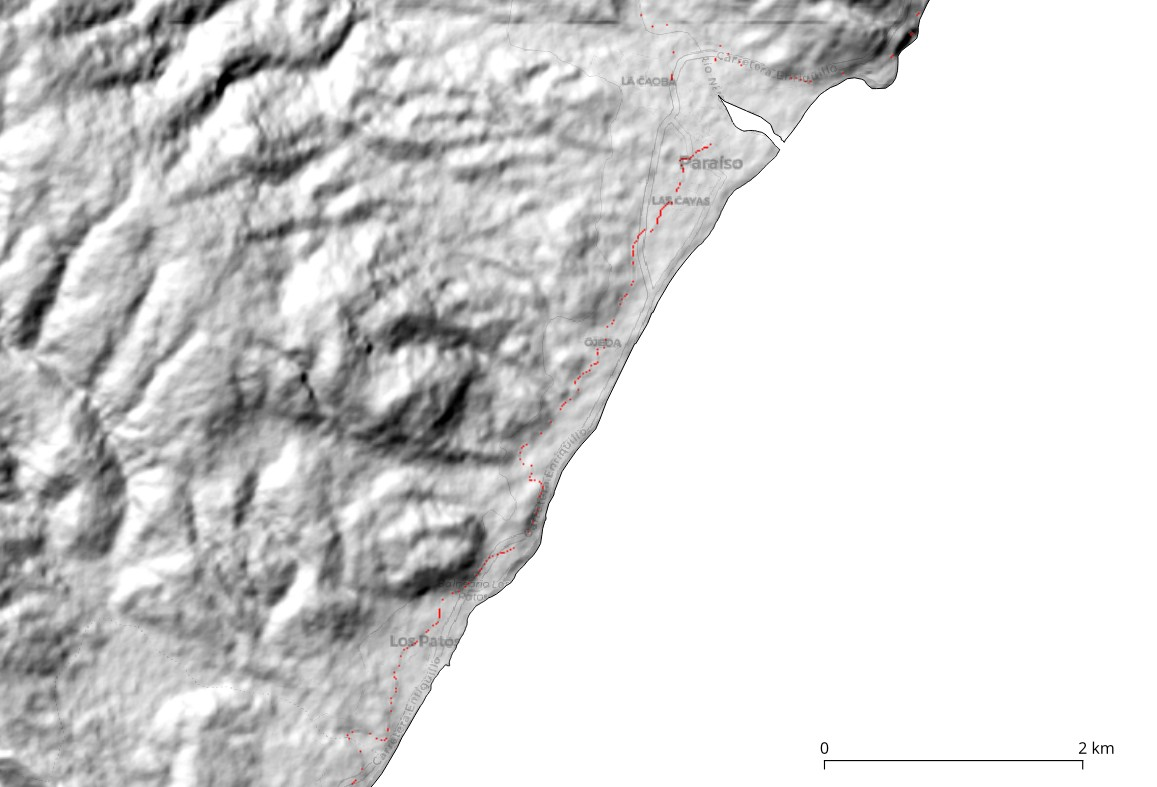
\includegraphics[width=0.8\linewidth]{figuras/dem-sin-procesar} 

}

\caption{DEM sin procesar, representado como relieve sombreado. Nótesense los píxeles sin datos, destacados en color rojo (Los Patos-Ojeda-Paraíso, provincia Barahona, sudoeste de República Dominicana)}\label{fig:demsinprocesar}
\end{figure}

A continuación, rellenamos las celdas con valor nulo (sin datos) por
medio del eficiente complemento de GRASS \texttt{r.fill.nulls}. Lo
configuramos para rellenar píxeles nulos usando interpolación
\emph{spline} bilineal con regularización Tykhonov (\emph{spline} es un
método de descomposición de curvas en porciones descritas por
polinomios).

\begin{Shaded}
\begin{Highlighting}[]
\CommentTok{\# Rellenar vacíos}
\BuiltInTok{time}\NormalTok{ r.fillnulls }\AttributeTok{{-}{-}overwrite} \AttributeTok{{-}{-}verbose} \DataTypeTok{\textbackslash{}}
\NormalTok{  input=dem method=}\StringTok{"bilinear"} \DataTypeTok{\textbackslash{}}
\NormalTok{  tension=40 smooth=0.1 edge=3 npmin=600 segmax=300 lambda=0.01 }\DataTypeTok{\textbackslash{}}
\NormalTok{  output=dem\_relleno}
\CommentTok{\# Enviar mensaje al finalizar (ejecutar conjuntamente con anterior)}
\BuiltInTok{echo} \StringTok{"Job finished"} \KeywordTok{|} \ExtensionTok{mail} \AttributeTok{{-}s} \StringTok{"Job finished"}\NormalTok{ USUARIO@MAIL}
\CommentTok{\#\# real 10m11.925s}
\end{Highlighting}
\end{Shaded}

\begin{figure}

{\centering 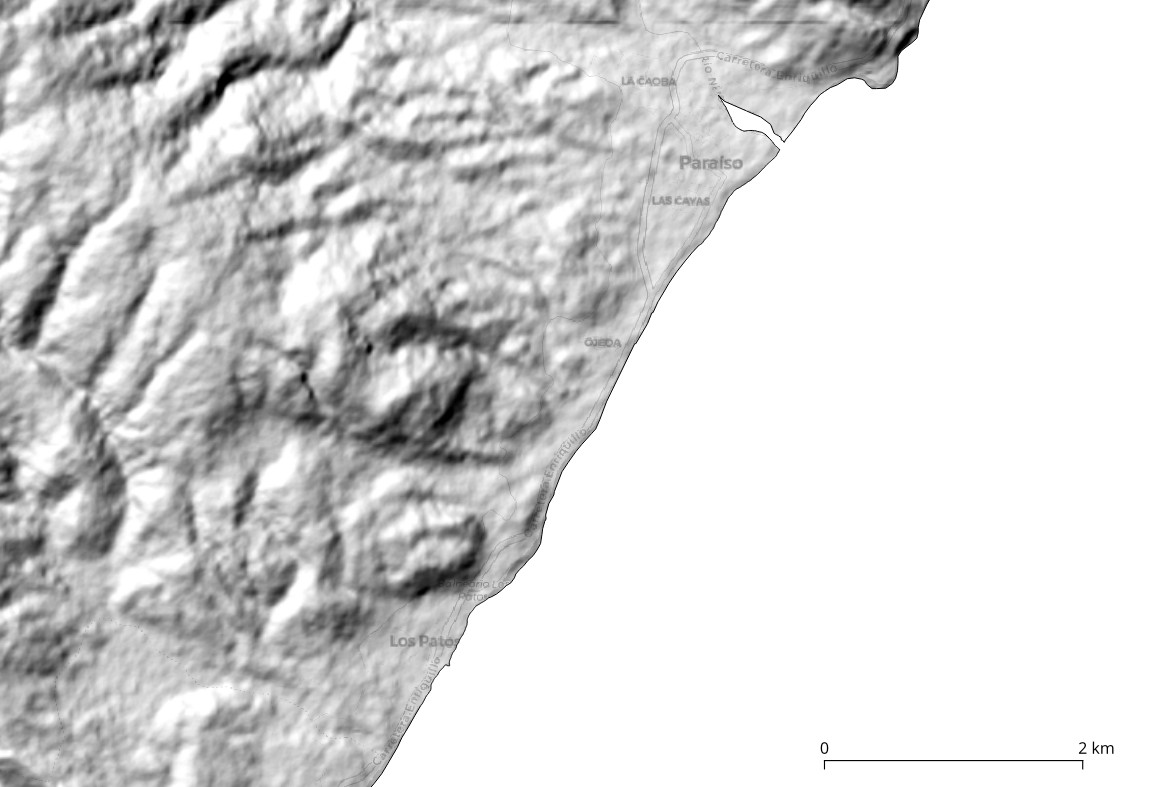
\includegraphics[width=0.8\linewidth]{figuras/dem-relleno} 

}

\caption{DEM sin procesar, representado como relieve sombreado. Los píxeles sin datos fueron eliminados (Los Patos-Ojeda-Paraíso, provincia Barahona, sudoeste de República Dominicana)}\label{fig:demrelleno}
\end{figure}

En el siguiente paso suavizamos el DEM preservando morfologías. Para
esto usamos la herramienta \emph{FeaturePreservingSmoothing} de
WhiteboxTools, la cual reduce la rugosidad generada por el ruido en el
DEM (Lindsay, 2018; Lindsay et~al., 2019). Para aplicar esta
herramienta, primero exportamos el DEM desde la base de datos de GRASS
GIS a archivo GeoTIFF, y posteriormente aplicamos el suavizado.
Finalmente, importamos el DEM suavizado nuevamente a la base de datos de
GRASS GIS para continuar el procesamiento en dicha aplicación.

\begin{Shaded}
\begin{Highlighting}[]
\CommentTok{\# Exportar a GTiff con compresión LZW}
\BuiltInTok{time}\NormalTok{ r.out.gdal }\AttributeTok{{-}{-}overwrite} \AttributeTok{{-}{-}verbose}\NormalTok{ createopt=}\StringTok{"COMPRESS=LZW,BIGTIFF=YES"} \DataTypeTok{\textbackslash{}}
\NormalTok{  input=dem\_relleno }\DataTypeTok{\textbackslash{}}
\NormalTok{  format=GTiff type=Float64 output=dem\_relleno.tif}
\CommentTok{\# Enviar mensaje al finalizar (ejecutar conjuntamente con anterior)}
\BuiltInTok{echo} \StringTok{"Job finished"} \KeywordTok{|} \ExtensionTok{mail} \AttributeTok{{-}s} \StringTok{"Job finished"}\NormalTok{ USUARIO@MAIL}
\CommentTok{\#\# real 0m58.924s}

\CommentTok{\# Comenzó a 23.20 de 22 de abril}
\BuiltInTok{time}\NormalTok{ \textasciitilde{}/WhiteboxTools\_linux\_amd64/WBT/whitebox\_tools }\DataTypeTok{\textbackslash{}}
  \AttributeTok{{-}{-}wd}\OperatorTok{=}\StringTok{\textquotesingle{}/media/jose/datos/alos{-}palsar{-}dem{-}rd/dem/\textquotesingle{}} \DataTypeTok{\textbackslash{}}
  \AttributeTok{{-}{-}filter}\OperatorTok{=}\NormalTok{25 }\AttributeTok{{-}{-}norm\_diff}\OperatorTok{=}\NormalTok{45 }\AttributeTok{{-}{-}num\_iter}\OperatorTok{=}\NormalTok{5 }\DataTypeTok{\textbackslash{}}
  \AttributeTok{{-}{-}run}\OperatorTok{=}\NormalTok{FeaturePreservingSmoothing }\AttributeTok{{-}{-}input}\OperatorTok{=}\StringTok{\textquotesingle{}dem\_relleno.tif\textquotesingle{}} \DataTypeTok{\textbackslash{}}
  \AttributeTok{{-}{-}output}\OperatorTok{=}\StringTok{\textquotesingle{}dem\_relleno\_suavizado.tif\textquotesingle{}} \AttributeTok{{-}v}
\CommentTok{\# Enviar mensaje al finalizar (ejecutar conjuntamente con anterior)}
\BuiltInTok{echo} \StringTok{"Job finished"} \KeywordTok{|} \ExtensionTok{mail} \AttributeTok{{-}s} \StringTok{"Job finished"}\NormalTok{ USUARIO@MAIL}
\CommentTok{\#\# real 9min46.103s}
\end{Highlighting}
\end{Shaded}

\begin{figure}

{\centering 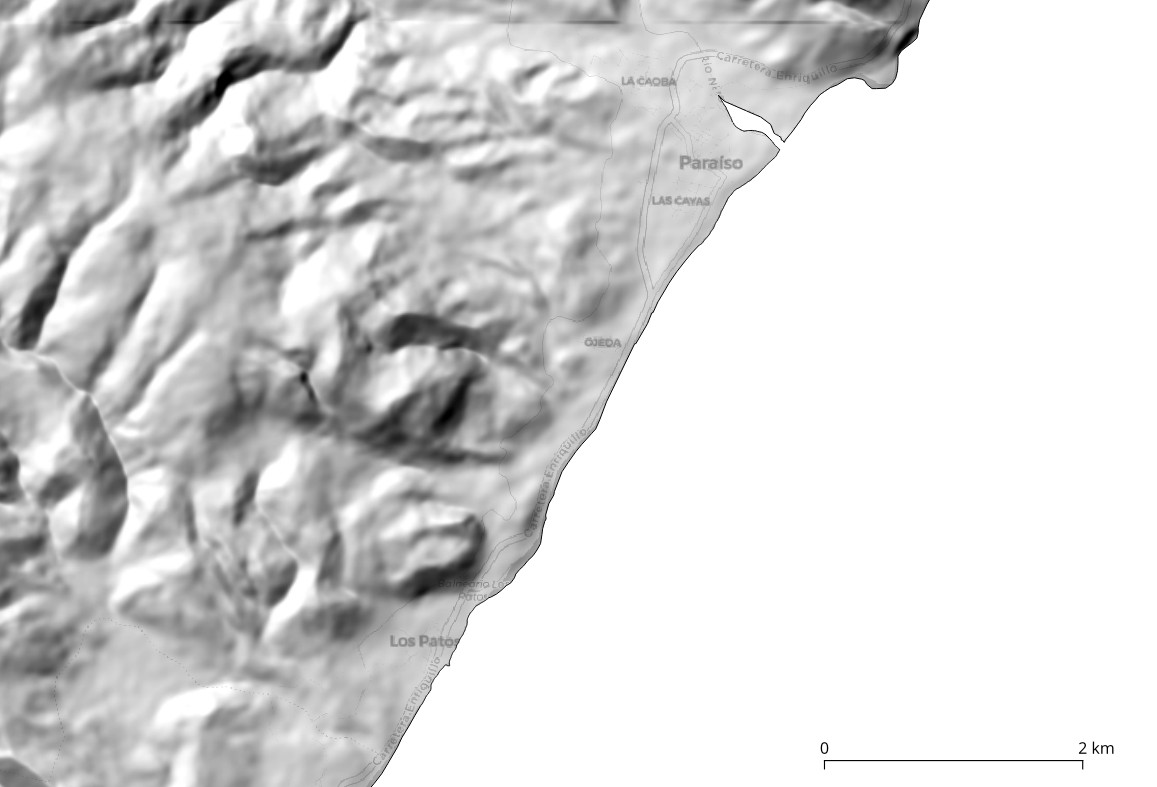
\includegraphics[width=0.8\linewidth]{figuras/dem-suavizado} 

}

\caption{DEM suavizado, representado como relieve sombreado. Nótese la conservación de las morfologías principales y la eliminación del ruido sobre éstas (Los Patos-Ojeda-Paraíso, provincia Barahona, sudoeste de República Dominicana)}\label{fig:demsuavizado}
\end{figure}

\begin{Shaded}
\begin{Highlighting}[]
\BuiltInTok{time}\NormalTok{ r.import input=dem\_relleno\_suavizado.tif output=dem\_suavizado}
\BuiltInTok{echo} \StringTok{"Job finished"} \KeywordTok{|} \ExtensionTok{mail} \AttributeTok{{-}s} \StringTok{"Job finished"}\NormalTok{ USUARIO@MAIL}
\CommentTok{\#\# real 0m21.593s}
\end{Highlighting}
\end{Shaded}

A continuación, usamos el ráster de altura de geoide de La Española a 1
minuto de resolución (EGM2008) para obtener alturas pseudo-ortométricas,
por medio de una suma algebraica simple de este ráster y el DEM
suavizado en GRASS GIS con la herramienta \texttt{r.mapcalc}. Sin
embargo, previamente fue necesario aumentar la resolución del ráster de
altura del geoide antes de realizar la suma. Para esto, usamos
\texttt{r.resamp.rst} (evaluamos una segunda alternativa con el
complemento \texttt{r.resamp.interp} y, aunque realizó el trabajo
eficientemente, eliminó muchas áreas limítrofes, por lo que preferimos
no utilizarlo).

\begin{Shaded}
\begin{Highlighting}[]
\CommentTok{\# Importar DEM a región de GRASS}
\ExtensionTok{r.import} \AttributeTok{{-}{-}overwrite}\NormalTok{ input=egm2008{-}1\_espanola.tif output=egm2008\_1min}

\CommentTok{\# Ver en lista (q para salir)}
\ExtensionTok{g.list}\NormalTok{ type=raster}

\CommentTok{\# Ver atributos de la región}
\ExtensionTok{g.region} \AttributeTok{{-}p}

\CommentTok{\# Alternativa 1. Usando r.resamp.rst. Más eficiente y precisa}
\CommentTok{\# Fijar la región al geoide importado}
\ExtensionTok{g.region}\NormalTok{ raster=egm2008\_1min }\AttributeTok{{-}ap}
\CommentTok{\# Realizar la interpolación}
\ExtensionTok{r.resamp.rst} \AttributeTok{{-}{-}overwrite}\NormalTok{ input=egm2008\_1min ew\_res=50 ns\_res=50 elevation=egm2008\_hires}
\BuiltInTok{echo} \StringTok{"Job finished"} \KeywordTok{|} \ExtensionTok{mail} \AttributeTok{{-}s} \StringTok{"Job finished"}\NormalTok{ USUARIO@MAIL}
\CommentTok{\#\# real }
\CommentTok{\# Fijar región a nuevo geoide}
\ExtensionTok{g.region}\NormalTok{ raster=egm2008\_hires }\AttributeTok{{-}ap}

\CommentTok{\# Alternativa 2. Usando r.resamp.interp. También eficiente, pero eliminar áreas de borde}
\CommentTok{\# g.region res=50 {-}ap}
\CommentTok{\# r.resamp.interp {-}{-}overwrite input=egm2008\_1min \textbackslash{}}
\CommentTok{\#  output=egm2008\_hires method=bilinear}

\CommentTok{\# Exportar para explorar visualmente}
\CommentTok{\# r.out.gdal {-}{-}overwrite {-}{-}verbose createopt="COMPRESS=LZW" \textbackslash{}}
\CommentTok{\#  input=egm2008\_hires \textbackslash{}}
\CommentTok{\#  format=GTiff type=Float64 output=egm2008\_hires.tif}

\CommentTok{\# Volver a resolución de DEM rellenado y suavizado}
\ExtensionTok{g.region}\NormalTok{ raster=dem\_suavizado }\AttributeTok{{-}ap}

\CommentTok{\# Aplicar álgebra de mapas}
\ExtensionTok{r.mapcalc} \AttributeTok{{-}{-}overwrite} \StringTok{"dem\_pseudo\_ortometrico = dem\_suavizado {-} egm2008\_hires"}

\CommentTok{\#Estadísticos univariados}
\ExtensionTok{r.univar} \AttributeTok{{-}{-}overwrite} \AttributeTok{{-}te} \DataTypeTok{\textbackslash{}}
\NormalTok{  map=dem\_pseudo\_ortometrico }\DataTypeTok{\textbackslash{}}
\NormalTok{  output=stats\_dem\_pseudo\_ortometrico.txt}
\end{Highlighting}
\end{Shaded}

\begin{Shaded}
\begin{Highlighting}[]
\NormalTok{stats\_dem\_pseudo\_ortometrico }\OtherTok{\textless{}{-}} \FunctionTok{read\_delim}\NormalTok{(}
  \FunctionTok{paste0}\NormalTok{(dem\_proc\_dir, }\StringTok{\textquotesingle{}/\textquotesingle{}}\NormalTok{,}
         \StringTok{\textquotesingle{}stats\_dem\_pseudo\_ortometrico.txt\textquotesingle{}}\NormalTok{),}
  \AttributeTok{progress =}\NormalTok{ F, }\AttributeTok{show\_col\_types =}\NormalTok{ F)}
\end{Highlighting}
\end{Shaded}

El resumen estadístico proporcionado por la herramienta
\texttt{r.univar} de GRASS GIS, usando la máscara ajustada a los límites
costeros e internacional del país, informó que la elevación mínima es
-51~m, mientras que la máxima es 3102~m, para un rango de casi 3154~m.
El valor mínimo probablemente no está bien recogido, debido a que la
máscara empleada podría estar eliminando elevaciones muy bajas en el
área de la Hoya de Enriquillo. La elevación media, considerando tanto
los negativos como los positivos, es de aproximadamente 404 m, con
desviación estándar de 487 m y coeficiente de variación de 121\%.
Remarcamos que, aunque ASF advierte de no usar este modelo para fines de
elevación, el valor máximo se ajusta bastante a la elevación máxima
conocida en República Dominicana, que es el pico Duarte (Instituto
Geográfico Nacional, 2022).

\begin{figure}

{\centering 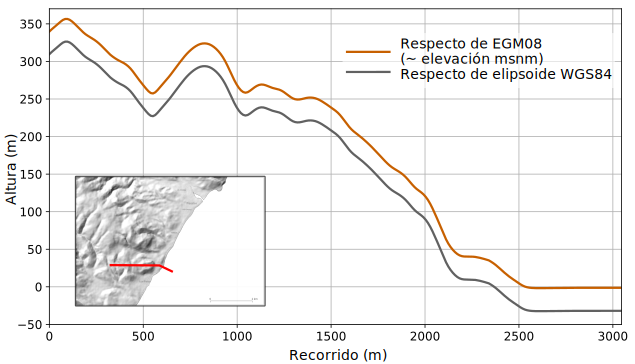
\includegraphics[width=0.8\linewidth]{figuras/perfiles-dem/los-patos} 

}

\caption{Alturas respecto de geoide EGM08 ($\sim$ortométrica) y sobre elipsoide WGS84, de un transecto descendente desde Bahoruco Oriental al Mar Caribe (Los Patos-Ojeda-Paraíso, provincia Barahona, sudoeste de República Dominicana)}\label{fig:alturasgeoideelipsoide}
\end{figure}

A continuación, efectuamos el procedimiento de tallado o grabado de una
red preexistente sobre el DEM, conocido como \emph{stream burning}
(Lindsay, 2016). Con este procedimiento, logramos que los píxeles del
DEM intersectados con el vectorial de la red preexistente, adquieran un
valor muy bajo respecto de su entorno, para asegurar que los algoritmos
automáticos de análisis hidrológico dirijan el flujo a través de los
lechos de ríos establecidos. El tallado es particularmente útil, incluso
esencial, en áreas planas, ya que ayuda a los algoritmos autómáticos a
producir redes hidrográficas más realistas y topológicamente correctas.
Sin embargo, su aplicación de requiere de una cuidadosa selección de la
red preexistente a tallar. Para crearla, usamos una red de drenaje de
cursos fluviales seleccionados, que incluyó sólo los de mayor longitud,
comúnmente ríos permamentes, de lecho ancho y claramente establecidos.
Nos apoyamos en imágenes satelitales (Google; Airbus, CNES; Airbus,
Landsat; Copernicus; Maxar Technologies; U.S. Geological Survey, 2023)
y, ocasionalmente, en el MTN-50K (Instituto Cartográfico Militar (ICM),
1989). Complementamos con OpenStreetMap contributors (2017), ya que este
servicio provee información vectorial de fácil acceso y precisa. El
resultado consistió en una red de cursos seleccionados para el tallado
del DEM, representada por los ríos Artibonito, Yaque del Norte, Yuna,
Yaque del Sur, varios ríos del extremo meridional de la cordillera
Central y del borde sudoriental del país, así como algunos ríos
seleccionados de la cordillera Septentrional.

\begin{figure}

{\centering 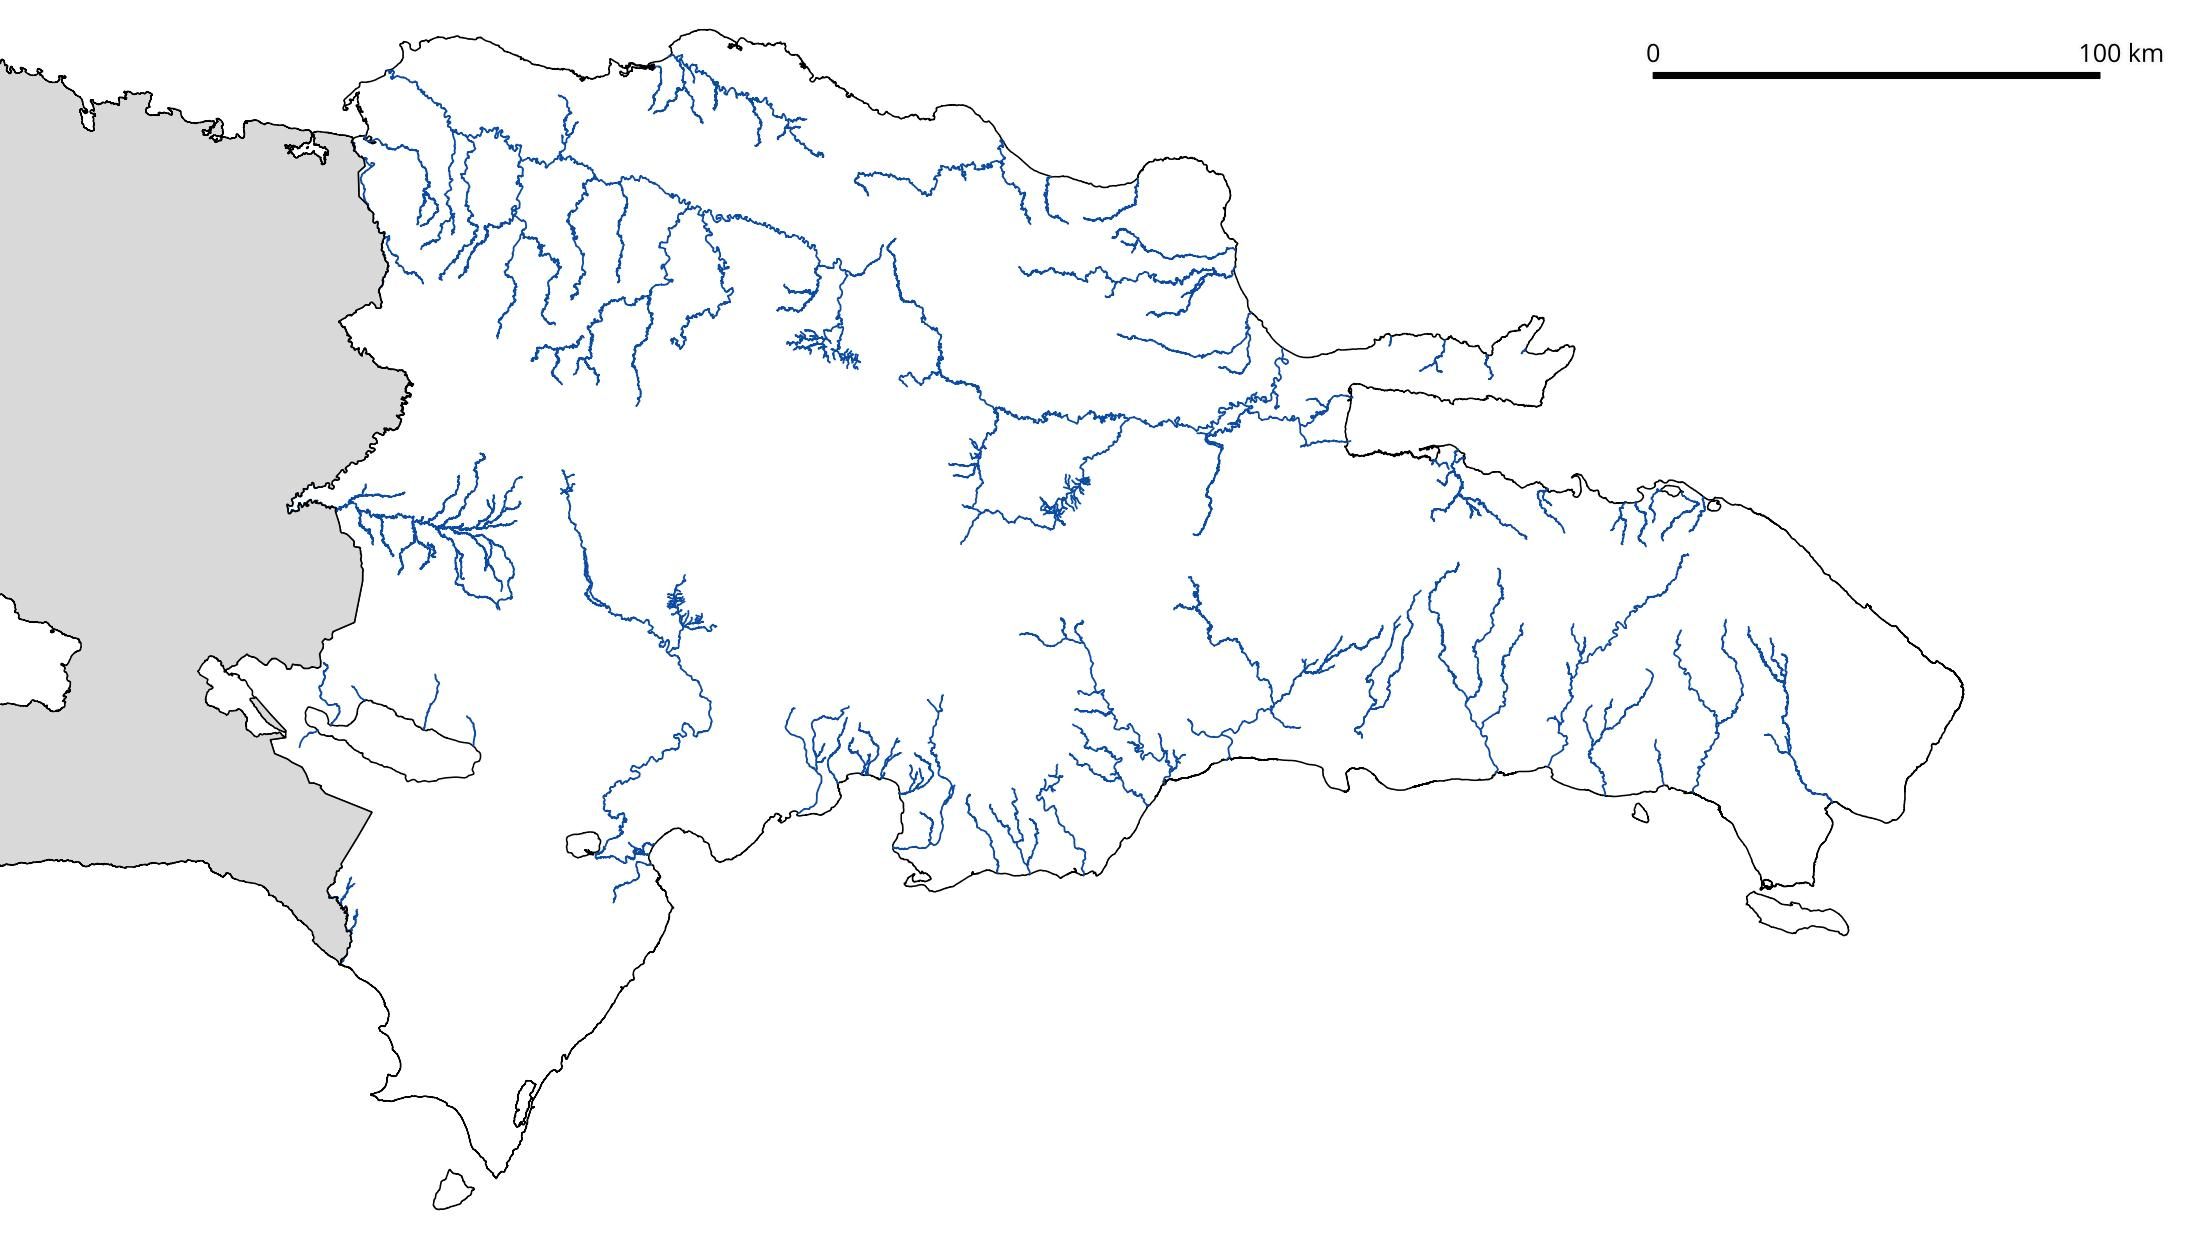
\includegraphics[width=0.8\linewidth]{figuras/red-cursos-largos} 

}

\caption{Mapa de la red de cursos largos creada para el estudio a partir de varias fuentes (más detalles, en el texto).}\label{fig:redcursoslargos}
\end{figure}

Nuestra de red cursos seleccionados para el tallado contiene varios ríos
que atraviesan amplios valles y karsts, por lo que son comunes los
tramos que cruzan zonas complicadas para la conducción del flujo donde
probablemente el error posicional de las líneas es mayor. Cabe también
señalar que, para asegurar la continuidad topológica de la red, dimos un
tratamiento especial a los ríos que llenan embalses, los cuales
representamos por medio trazados históricos obtenidos del MTN-50K,
omitiendo así la presencia de los embalses.

\begin{Shaded}
\begin{Highlighting}[]
\CommentTok{\# Importar red a GRASS}
\CommentTok{\# IMPORTANTE: la red en el GPKG que se desea tallar, debe tener "1" en el campo "rasterizar"}
\ExtensionTok{v.import} \AttributeTok{{-}{-}overwrite}\NormalTok{ input=red\_mtn50k\_cleaned\_largos.gpkg }\DataTypeTok{\textbackslash{}}
\NormalTok{  output=red\_mtn50k\_cleaned\_largos}
\CommentTok{\# Ver mapa importado en lista (q para salir)}
\ExtensionTok{g.list}\NormalTok{ type=vector}
\CommentTok{\# Calcular y pasar a archivo, la longitud de cursos}
\CommentTok{\# y número de segmentos (ejecutar en casos de actualización)}
\ExtensionTok{v.to.db} \AttributeTok{{-}p}\NormalTok{ option=length map=red\_mtn50k\_cleaned\_largos }\OperatorTok{\textgreater{}} \DataTypeTok{\textbackslash{}}
\NormalTok{  stats\_length\_red\_mtn50k\_cleaned\_largos.txt}
\end{Highlighting}
\end{Shaded}

\begin{Shaded}
\begin{Highlighting}[]
\NormalTok{stats\_red\_mtn50k\_largos }\OtherTok{\textless{}{-}} \FunctionTok{read\_delim}\NormalTok{(}
  \FunctionTok{paste0}\NormalTok{(dem\_proc\_dir, }\StringTok{\textquotesingle{}/\textquotesingle{}}\NormalTok{,}
         \StringTok{\textquotesingle{}stats\_length\_red\_mtn50k\_cleaned\_largos.txt\textquotesingle{}}\NormalTok{),}
  \AttributeTok{progress =}\NormalTok{ F, }\AttributeTok{show\_col\_types =}\NormalTok{ F)}
\NormalTok{n\_seg\_red\_mtn50k\_largos }\OtherTok{\textless{}{-}}\NormalTok{ stats\_red\_mtn50k\_largos }\SpecialCharTok{\%\textgreater{}\%}
  \FunctionTok{filter}\NormalTok{(}\SpecialCharTok{!}\NormalTok{cat}\SpecialCharTok{=={-}}\DecValTok{1}\NormalTok{) }\SpecialCharTok{\%\textgreater{}\%}\NormalTok{ nrow}
\NormalTok{length\_mtn50k\_largos }\OtherTok{\textless{}{-}}\NormalTok{ stats\_red\_mtn50k\_largos }\SpecialCharTok{\%\textgreater{}\%}
  \FunctionTok{filter}\NormalTok{(}\SpecialCharTok{!}\NormalTok{cat}\SpecialCharTok{=={-}}\DecValTok{1}\NormalTok{) }\SpecialCharTok{\%\textgreater{}\%} \FunctionTok{pull}\NormalTok{(length) }\SpecialCharTok{\%\textgreater{}\%}\NormalTok{ sum}\SpecialCharTok{/}\DecValTok{1000}
\end{Highlighting}
\end{Shaded}

Finalmente, importamos nuestra red de cursos seleccionados para el
tallado a la base de datos de GRASS GIS y generamos estadísticas
básicas. Se trata de una red compuesta por \textbf{388 segmentos} que
suman un total de \textbf{5163.66 kilómetros} de longitud. Cabe señalar
que esta red no tiene valor hidrográfico, pues, como indicamos, ignora
los lagos para garantizar la integridad topológica. Desaconsejamos su
uso para otro fin que no sea el grabado de un DEM.

El siguiente paso consistió en realizar el \emph{stream burning}
(tallado) de la red de cursos seleccionados, usando distintos algoritmos
sobre el DEM. Probamos las funciones \texttt{r.carve} y
\texttt{r.mapcalc} (álgebra de mapas) de GRASS GIS, y \texttt{FillBurn}
de WhiteboxTools (GRASS Development Team, 2022a; Lindsay, 2018). Sin
embargo, es importante señalar que, dependiendo del algoritmo usado, el
grabado modifica de forma diferente el DEM. Además, algunos algoritmos
modifican no solamente los píxeles intersectados sino también otros
píxeles, incluso pueden llegar a cambiar los valores en el DEM completo.
Nosotros priorizamos un método de grabado que fuese efectivo pero que a
la vez produjese la mínima alteración sobre el DEM.

Comenzamos con \texttt{r.carve}, una herramienta diseñada para grabar el
DEM sin modificarlo sustancialmente, permitiendo al mismo tiempo
configurar la profundidad y la anchura del grabado (GRASS Development
Team, 2022b; Petrasova et~al., 2011). Por defecto, la anchura de lecho
es equivalente a la resolución del DEM. La profundidad puede definirse
por el usuario, para lo cual nosotros establecimos 100 metros. Pudimos
tallar la red de cursos seleccionados sobre el DEM con esta herramienta,
generando un resultado que consideramos bueno, aunque el proceso ocupó
más de 1 hora de tiempo de cómputo. Esta alternativa es recomendada si
resultase imprescindible conservar las propiedades topográficas en el
DEM, pero debe tenerse en cuenta que su rendimiento es muy bajo. En los
casos en los que se use un DEM de resolución baja, se recomienda usar
esta alternativa. Sin embargo, a nosotros no nos resultó apropiado este
método por razones de rendimiento, que explicamos a continuación. Para
evaluar el rendimiento del DEM tallado, realizábamos un procesamiento
hidrológico abreviado (generación de la acumulación de flujo y
extracción de la red con \texttt{r.watershed}); si los productos
generados (e.g.~red hidrográfica) no nos parecían idóneos, nos veíamos
en la necesidad iterar, editando la red y aplicando el tallado
nuevamente. Dado que el complemento \texttt{r.carve} era poco eficiente,
preferimos buscar otras opciones de tallado.

\begin{Shaded}
\begin{Highlighting}[]
\CommentTok{\# Tallar red de cursos seleccionados usando r.carve (ALTERNATIVA DESCARTADA)}
\CommentTok{\# Limpiar red manualmente en QGIS}
\CommentTok{\#\# Adicionalmente, para mejorar la topología, se puede aplicar}
\CommentTok{\#\# v.clean directamente en QGIS, o hacerlo en GRASS GIS tras importar}
\CommentTok{\# Aplicar r.carve}
\CommentTok{\# time r.carve {-}{-}overwrite {-}{-}verbose raster=dem\_pseudo\_ortometrico \textbackslash{}}
\CommentTok{\#   vector=red\_mtn50k\_cleaned\_largos output=dem\_tallado depth=100}
\CommentTok{\# echo "r.carve finalizado" | mail {-}s "r.carve finalizado" USUARIO@MAIL}
\CommentTok{\#\# real 97m3.970s}
\end{Highlighting}
\end{Shaded}

Posteriormente, probamos el tallado usando álgebra de mapas con
herramienta \texttt{r.mapcalc} de GRASS GIS (GRASS Development Team,
2022a; GRASS Development Team, 2022c; Larson et~al., 1991; Shapiro y
Westervelt, 1994). Para tallar con álgebra de mapas, primero
normalizamos el DEM, generamos una capa booleana ráster con la red de
cursos seleccionados, la restamos al DEM normalizado y luego, para
restablecer los valores originales fuera de las áreas talladas,
multiplicamos el ráster resultante de la resta nuevamente por el rango
del DEM (máximo - mínimo). El resultado es un DEM tallado, en el que
sólo los píxeles por donde circula la red quedaron con una profundidad
equivalente al rango. Esta alternativa fue la seleccionada por ser la
más eficiente y que menor modificación introdujo en el DEM.

\begin{Shaded}
\begin{Highlighting}[]
\CommentTok{\# Tallar con álgebra de mapas (ALTERNATIVA ELEGIDA)}
\CommentTok{\# Antes de comenzar, limpiar red manualmente en QGIS}
\CommentTok{\# Para mejorar la topología, se puede aplicar v.clean directamente en QGIS}
\CommentTok{\# Primero, rasterizar red (los píxeles de la red valdrán 1, el resto, nulo)}
\ExtensionTok{v.to.rast} \AttributeTok{{-}{-}overwrite} \DataTypeTok{\textbackslash{}}
\NormalTok{  input=red\_mtn50k\_cleaned\_largos type=line use=attr }\DataTypeTok{\textbackslash{}}
\NormalTok{  attribute\_column=rasterizar }\DataTypeTok{\textbackslash{}}
\NormalTok{  output=red\_mtn50k\_cleaned\_largos }\DataTypeTok{\textbackslash{}}
\NormalTok{  memory=32000}
\CommentTok{\# La columna "rasterizar" es 0 para cursos que no se rasterizan}
\CommentTok{\# Luego convertir nulos a cero}
\ExtensionTok{r.null}\NormalTok{ map=red\_mtn50k\_cleaned\_largos null=0}
\CommentTok{\# A continuación, determinar estadísticas univariantes del DEM}
\CommentTok{\# confirmar que no sufre gran modificación de sus valores extremos}
\ExtensionTok{r.univar}\NormalTok{ map=dem\_pseudo\_ortometrico}
\CommentTok{\# minimum: {-}51.4456}
\CommentTok{\# maximum: 3102.34}
\CommentTok{\# Finalmente, aplicar el tallado mediante normalización y resta con r.mapcalc}
\BuiltInTok{time}\NormalTok{ r.mapcalc }\AttributeTok{{-}{-}overwrite} \OperatorTok{\textless{}\textless{} EOF}
\StringTok{eval(stddem = (dem\_pseudo\_ortometrico {-} {-}51.4456) / (3102.34 {-} {-}51.4456), }\DataTypeTok{\textbackslash{}}
\StringTok{     stddemburn = stddem {-} red\_mtn50k\_cleaned\_largos)}
\StringTok{dem\_tallado = (stddemburn * (3102.34 {-} {-}51.4456)) {-} 51.4456}
\OperatorTok{EOF}
\BuiltInTok{echo} \StringTok{"Tallado finalizado"} \KeywordTok{|} \ExtensionTok{mail} \AttributeTok{{-}s} \StringTok{"Mensaje sobre tallado"}\NormalTok{ USUARIO@MAIL}
\CommentTok{\#\# real 1m5.194s}
\CommentTok{\# A continuación, determinar estadísticas univariantes del DEM}
\CommentTok{\# confirmar que no sufre gran modificación de sus valores extremos}
\ExtensionTok{r.univar}\NormalTok{ map=dem\_pseudo\_ortometrico}
\end{Highlighting}
\end{Shaded}

\begin{figure}

{\centering 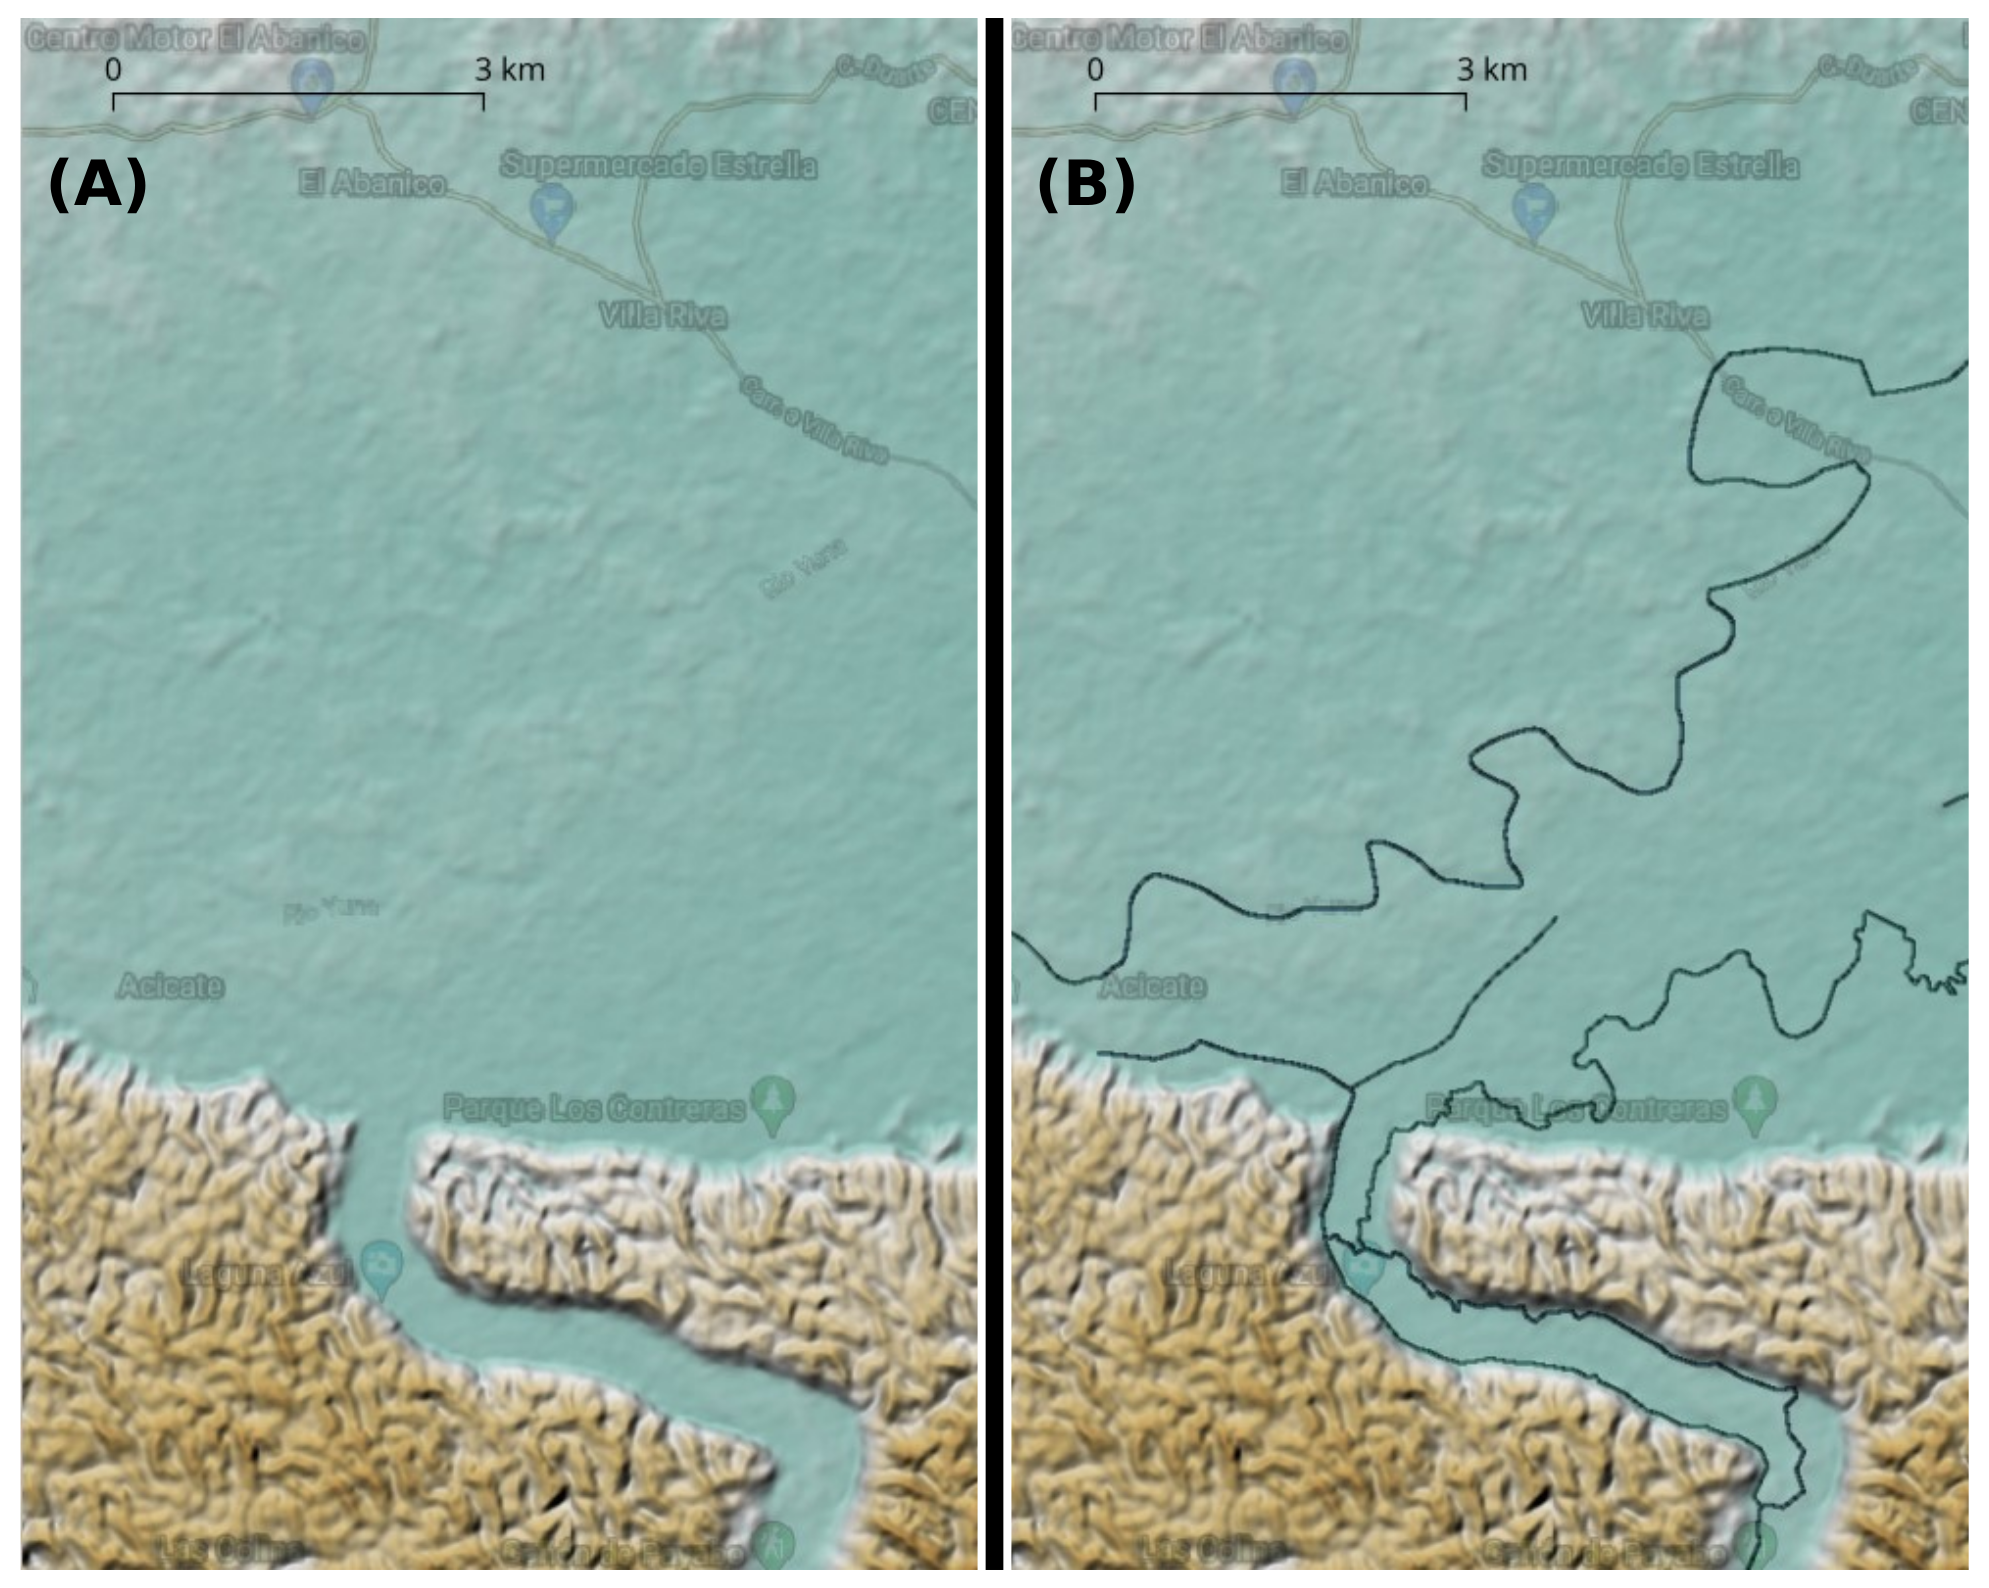
\includegraphics[width=0.8\linewidth]{figuras/dem-sin-tallar-tallado} 

}

\caption{DEM sin aplicación de hidrografía (A), y con aplicación de hidrografía seleccionada o "DEM tallado" (B). El DEM se representa como relieve sombreado y la aplicación se denota como un grabado oscurecido (cañón del río Payabo, Los Haitises, y río Yuna (proximidades de Arenoso, nordeste de República Dominicana)}\label{fig:demtallado}
\end{figure}

Como última alternativa de procesamiento, probamos la herramienta
\texttt{FillBurn}, basada en Saunders (2000) e implementada por Lindsay
(2016) en de WBT. \texttt{FillBurn} realiza dos modificaciones a la vez
sobre el DEM; por una parte, graba la red, usando una profundidad por
defecto y, por otro, rellena las depresiones. La herramienta mostró
mejor rendimiento que la de GRASS GIS en cuanto a tiempo de cómputo.
Tras tallar la red evaluamos el DEM resultante, y comprobamos que
\textbf{resultó ser muy diferente al original, especialmente en las
áreas con depresiones}. Por esta razón, descartamos este DEM y elegimos
usar el tallado por medio de álgebra de mapas (\texttt{r.mapcalc}) con
GRASS GIS en los siguientes pasos de nuestro flujo de trabajo.

\begin{Shaded}
\begin{Highlighting}[]
\CommentTok{\# Tallar con FillBurn de WhiteboxTools  (ALTERNATIVA DESCARTADA)}
\CommentTok{\# Exportar dem\_pseudo\_ortometrico a GTiff con compresión LZW}
\CommentTok{\# time r.out.gdal {-}{-}overwrite {-}{-}verbose createopt="COMPRESS=LZW,BIGTIFF=YES" \textbackslash{}}
\CommentTok{\#  input=dem\_pseudo\_ortometrico \textbackslash{}}
\CommentTok{\#  format=GTiff type=Float64 output=dem\_pseudo\_ortometrico.tif}
\CommentTok{\# echo "Job finished" | mail {-}s "Job finished" USUARIO@MAIL}
\CommentTok{\#\# real 1m0.248s}
\end{Highlighting}
\end{Shaded}

\begin{Shaded}
\begin{Highlighting}[]
\CommentTok{\# Exportar red\_mtn50k\_cleaned\_largos.gpkg a shapefile}
\CommentTok{\# ogr2ogr(}
\CommentTok{\#   src\_datasource\_name = paste0(\textquotesingle{}/media/jose/datos/alos{-}palsar{-}dem{-}rd/\textquotesingle{},}
\CommentTok{\#                                \textquotesingle{}dem/red\_mtn50k\_cleaned\_largos.gpkg\textquotesingle{}),}
\CommentTok{\#   dst\_datasource\_name = paste0(\textquotesingle{}/media/jose/datos/alos{-}palsar{-}dem{-}rd/\textquotesingle{},}
\CommentTok{\#                                \textquotesingle{}dem/red\_mtn50k\_cleaned\_largos.shp\textquotesingle{}),}
\CommentTok{\#   verbose=TRUE)}
\end{Highlighting}
\end{Shaded}

\begin{Shaded}
\begin{Highlighting}[]
\CommentTok{\# Tallar finalmente}
\CommentTok{\# time \textasciitilde{}/WhiteboxTools\_linux\_amd64/WBT/whitebox\_tools \textbackslash{}}
\CommentTok{\#   {-}{-}wd=\textquotesingle{}/media/jose/datos/alos{-}palsar{-}dem{-}rd/dem/\textquotesingle{} \textbackslash{}}
\CommentTok{\#   {-}{-}run=FillBurn {-}{-}dem=\textquotesingle{}dem\_pseudo\_ortometrico.tif\textquotesingle{} \textbackslash{}}
\CommentTok{\#   {-}{-}streams=red\_mtn50k\_cleaned.shp {-}{-}output=\textquotesingle{}dem\_tallado.tif\textquotesingle{} {-}v}
\CommentTok{\# echo "Job finished" | mail {-}s "Job finished" USUARIO@MAIL}
\CommentTok{\#\# real 9m21.980s}
\CommentTok{\# Importar a GRASS GIS}
\CommentTok{\# time r.import {-}{-}overwrite input=dem\_tallado.tif output=dem\_tallado}
\CommentTok{\# echo "Job finished" | mail {-}s "Job finished" USUARIO@MAIL}
\CommentTok{\#\# real 0m38.519s}
\end{Highlighting}
\end{Shaded}

A continuación, implementamos algoritmos para superponer depresiones
sobre el Modelo Digital de Elevación (DEM). Este paso es esencial para
guiar el flujo de agua a través de las depresiones, en los lugares donde
éstas sean presentes. Es importante tener en cuenta que sólo se deben
superponer aquellas depresiones que tengan la capacidad de capturar la
escorrentía superficial, como los ponores o pérdidas, ya que son estos
elementos los que condicionarán la hidrología en su entorno. El proceso
de superposición de depresiones es fundamental para obtener límites de
cuencas y redes de drenaje coherentes.

Para generar un conjunto de depresiones, utilizamos la capa de
litologías de la República Dominicana, proporcionada por Mollat et~al.
(2004). A partir de este recurso, identificamos y separamos las calizas
que presentaban un grado de karstificación suficiente, basándonos en
nuestra experiencia de campo. Además, creamos una capa de depresiones
empleando el complemento \texttt{r.geomorphon} y utilizando el DEM como
insumo, según el método propuesto por Jasiewicz y Stepinski (2013).
También digitalizamos manualmente algunas depresiones cuya ubicación ya
conocíamos a partir de nuestra experiencia en el terreno. Finalmente,
realizamos una intersección de las tres fuentes de datos para producir
una capa exhaustiva que refleja las depresiones capaces de capturar el
flujo superficial.

\begin{figure}

{\centering 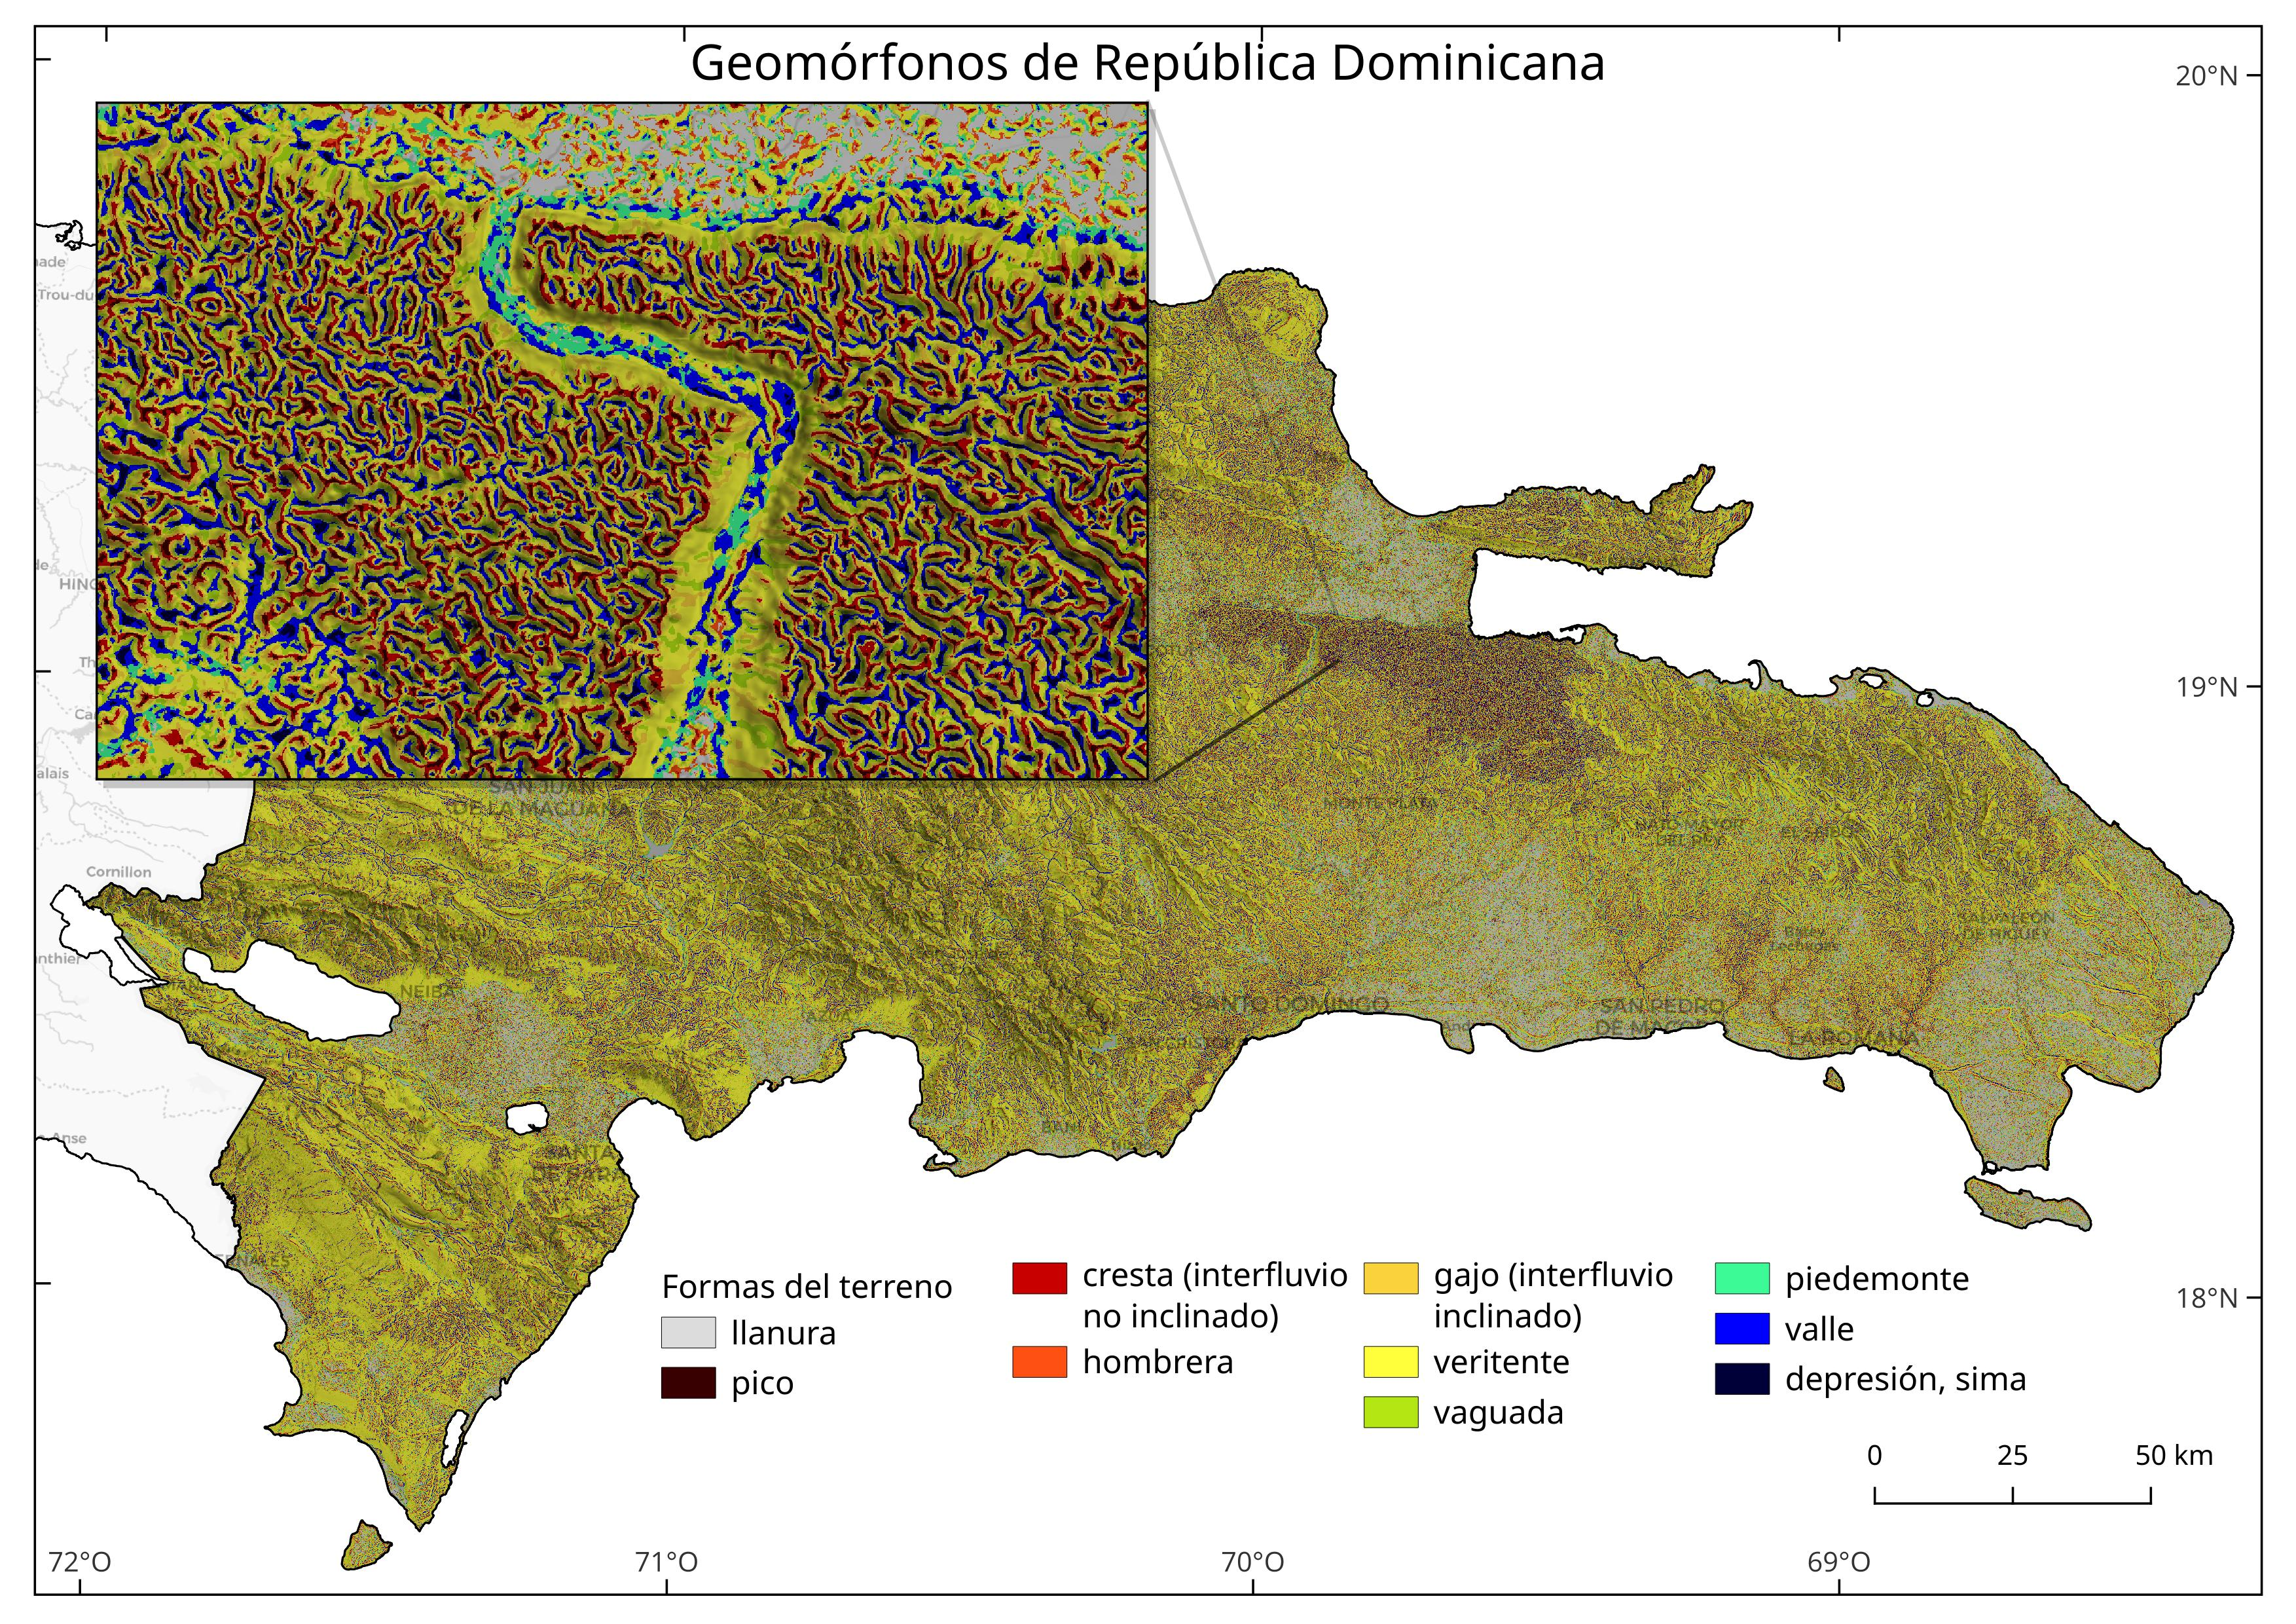
\includegraphics[width=0.8\linewidth]{figuras/geomorfonos-de-rd} 

}

\caption{"Geomórfonos" de República Dominicana generados a partir de DEM ALOS PALSAR. En cartela, detalle del cañón del río Payabo}\label{fig:geomorfonosrd}
\end{figure}

No obstante, nuestro resultado debe tomarse con cautela en el relieve
kárstico. Como bien es sabido, no todas las calizas representadas en la
geología dominicana están lo suficientemente karstificadas como para
desarrollar depresiones. Por esta razón, usamos la capa de calizas a
discreción, y sólo conservamos aquellos afloramientos de calizas en los
que, desde nuestro conocimiento de terreno, no se evidenciaba
escorrentía superficial. Asimismo, reservamos aquellas calizas donde
encontramos evidencia de depresiones en la topografía detallada y en
imágenes satelitales. No obstante, gran parte de este trabajo se realizó
manualmente, por lo que nuestra colección de dolinas tiene suficiente
precisión, pero no es exhaustiva. Además, es virtualmente imposible
identificar todas las depresiones que funcionan como pérdidas en
imágenes satelitales o en mapas topográficos y geológicos. Finalmente,
un elemento adicional complica aún más las cosas en los relieves
kársticos: muchas pérdidas no ocurren a través de una depresión
topográficamente visible, pues gran parte de la infiltración se produce
a través de fracturas en la roca, pasando al endokarst y a la zona
vadosa de manera ``silenciosa'', sin que veamos desde el aire la típica
morfología deprimida (e.g.~dolina).

\begin{Shaded}
\begin{Highlighting}[]
\CommentTok{\# Crear geomórfonos}
\CommentTok{\# WBT}
\CommentTok{\# time \textasciitilde{}/WhiteboxTools\_linux\_amd64/WBT/whitebox\_tools \textbackslash{}}
\CommentTok{\#   {-}r=Geomorphons {-}v {-}{-}wd=\textquotesingle{}/media/jose/datos/alos{-}palsar{-}dem{-}rd/dem/\textquotesingle{} \textbackslash{}}
\CommentTok{\#   {-}{-}dem=dem\_pseudo\_ortometrico.tif {-}o=geomorfonos.tif {-}{-}search=25 \textbackslash{}}
\CommentTok{\#   {-}{-}threshold=0 {-}{-}tdist=0.0 {-}{-}forms}
\CommentTok{\# echo "Job finished" | mail {-}s "Job finished" USUARIO@MAIL}
\CommentTok{\#\# real 6m52.298s \#MUY EFICIENTE. Se prefirió la versión de GRASS }
\CommentTok{\#\# para garantizar flujo de trabajo dentro de la base de datos.}
\CommentTok{\# GRASS GIS}
\BuiltInTok{time}\NormalTok{ r.geomorphon }\DataTypeTok{\textbackslash{}}
  \AttributeTok{{-}{-}overwrite} \AttributeTok{{-}{-}verbose} \DataTypeTok{\textbackslash{}}
\NormalTok{  elevation=dem\_pseudo\_ortometrico forms=geomorfonos search=25}
\BuiltInTok{echo} \StringTok{"r.geomorphon finalizado"} \KeywordTok{|} \ExtensionTok{mail} \AttributeTok{{-}s} \StringTok{"Mensaje sobre r.geomorphon"}\NormalTok{ USUARIO@MAIL}
\CommentTok{\#\# real 33m16.508s \#MUY LENTO}

\CommentTok{\# Extraer depresiones desde geomorfonos}
\ExtensionTok{r.mapcalc} \AttributeTok{{-}{-}overwrite} \DataTypeTok{\textbackslash{}}
\NormalTok{  expression=}\StringTok{"\textquotesingle{}depresiones\_geomorfonos\textquotesingle{} = if(geomorfonos == 10, 1, null())"}

\CommentTok{\# Importar depresiones manualmente digitalizadas a base de datos de GRASS GIS}
\ExtensionTok{v.import} \AttributeTok{{-}{-}overwrite}\NormalTok{ input=depresiones\_digitalizadas.gpkg }\DataTypeTok{\textbackslash{}}
\NormalTok{  output=depresiones\_digitalizadas}

\CommentTok{\# Convertir depresiones digitalizadas manualmente a ráster}
\ExtensionTok{v.to.rast} \AttributeTok{{-}{-}overwrite}\NormalTok{ input=depresiones\_digitalizadas }\DataTypeTok{\textbackslash{}}
\NormalTok{  type=area use=val output=depresiones\_digitalizadas}

\CommentTok{\# Importar la capa de calizas con depresiones en RD (de Mapa Geológico 250K)}
\ExtensionTok{v.import} \AttributeTok{{-}{-}overwrite}\NormalTok{ input=calizas\_con\_depresiones.gpkg output=calizas\_con\_depresiones}

\CommentTok{\# Convertir la capa de calizas con depresiones a ráster}
\ExtensionTok{v.to.rast} \AttributeTok{{-}{-}overwrite}\NormalTok{ input=calizas\_con\_depresiones type=area }\DataTypeTok{\textbackslash{}}
\NormalTok{  use=val output=calizas\_con\_depresiones}

\CommentTok{\# Adjuntar depresiones digitalizadas manualmente con calizas}
\ExtensionTok{r.mapcalc} \AttributeTok{{-}{-}overwrite} \DataTypeTok{\textbackslash{}}
\NormalTok{  expression=}\StringTok{"\textquotesingle{}depresiones\_geomorfonos\_calizas\textquotesingle{} = }\DataTypeTok{\textbackslash{}}
\StringTok{              \textquotesingle{}depresiones\_geomorfonos\textquotesingle{} * \textquotesingle{}calizas\_con\_depresiones\textquotesingle{}"}

\CommentTok{\# Unir todas las depresiones en un único mapa}
\ExtensionTok{r.patch} \AttributeTok{{-}{-}overwrite}\NormalTok{ input=depresiones\_geomorfonos\_calizas,depresiones\_digitalizadas }\DataTypeTok{\textbackslash{}}
\NormalTok{  output=depresiones\_todas}
\end{Highlighting}
\end{Shaded}

\begin{figure}

{\centering 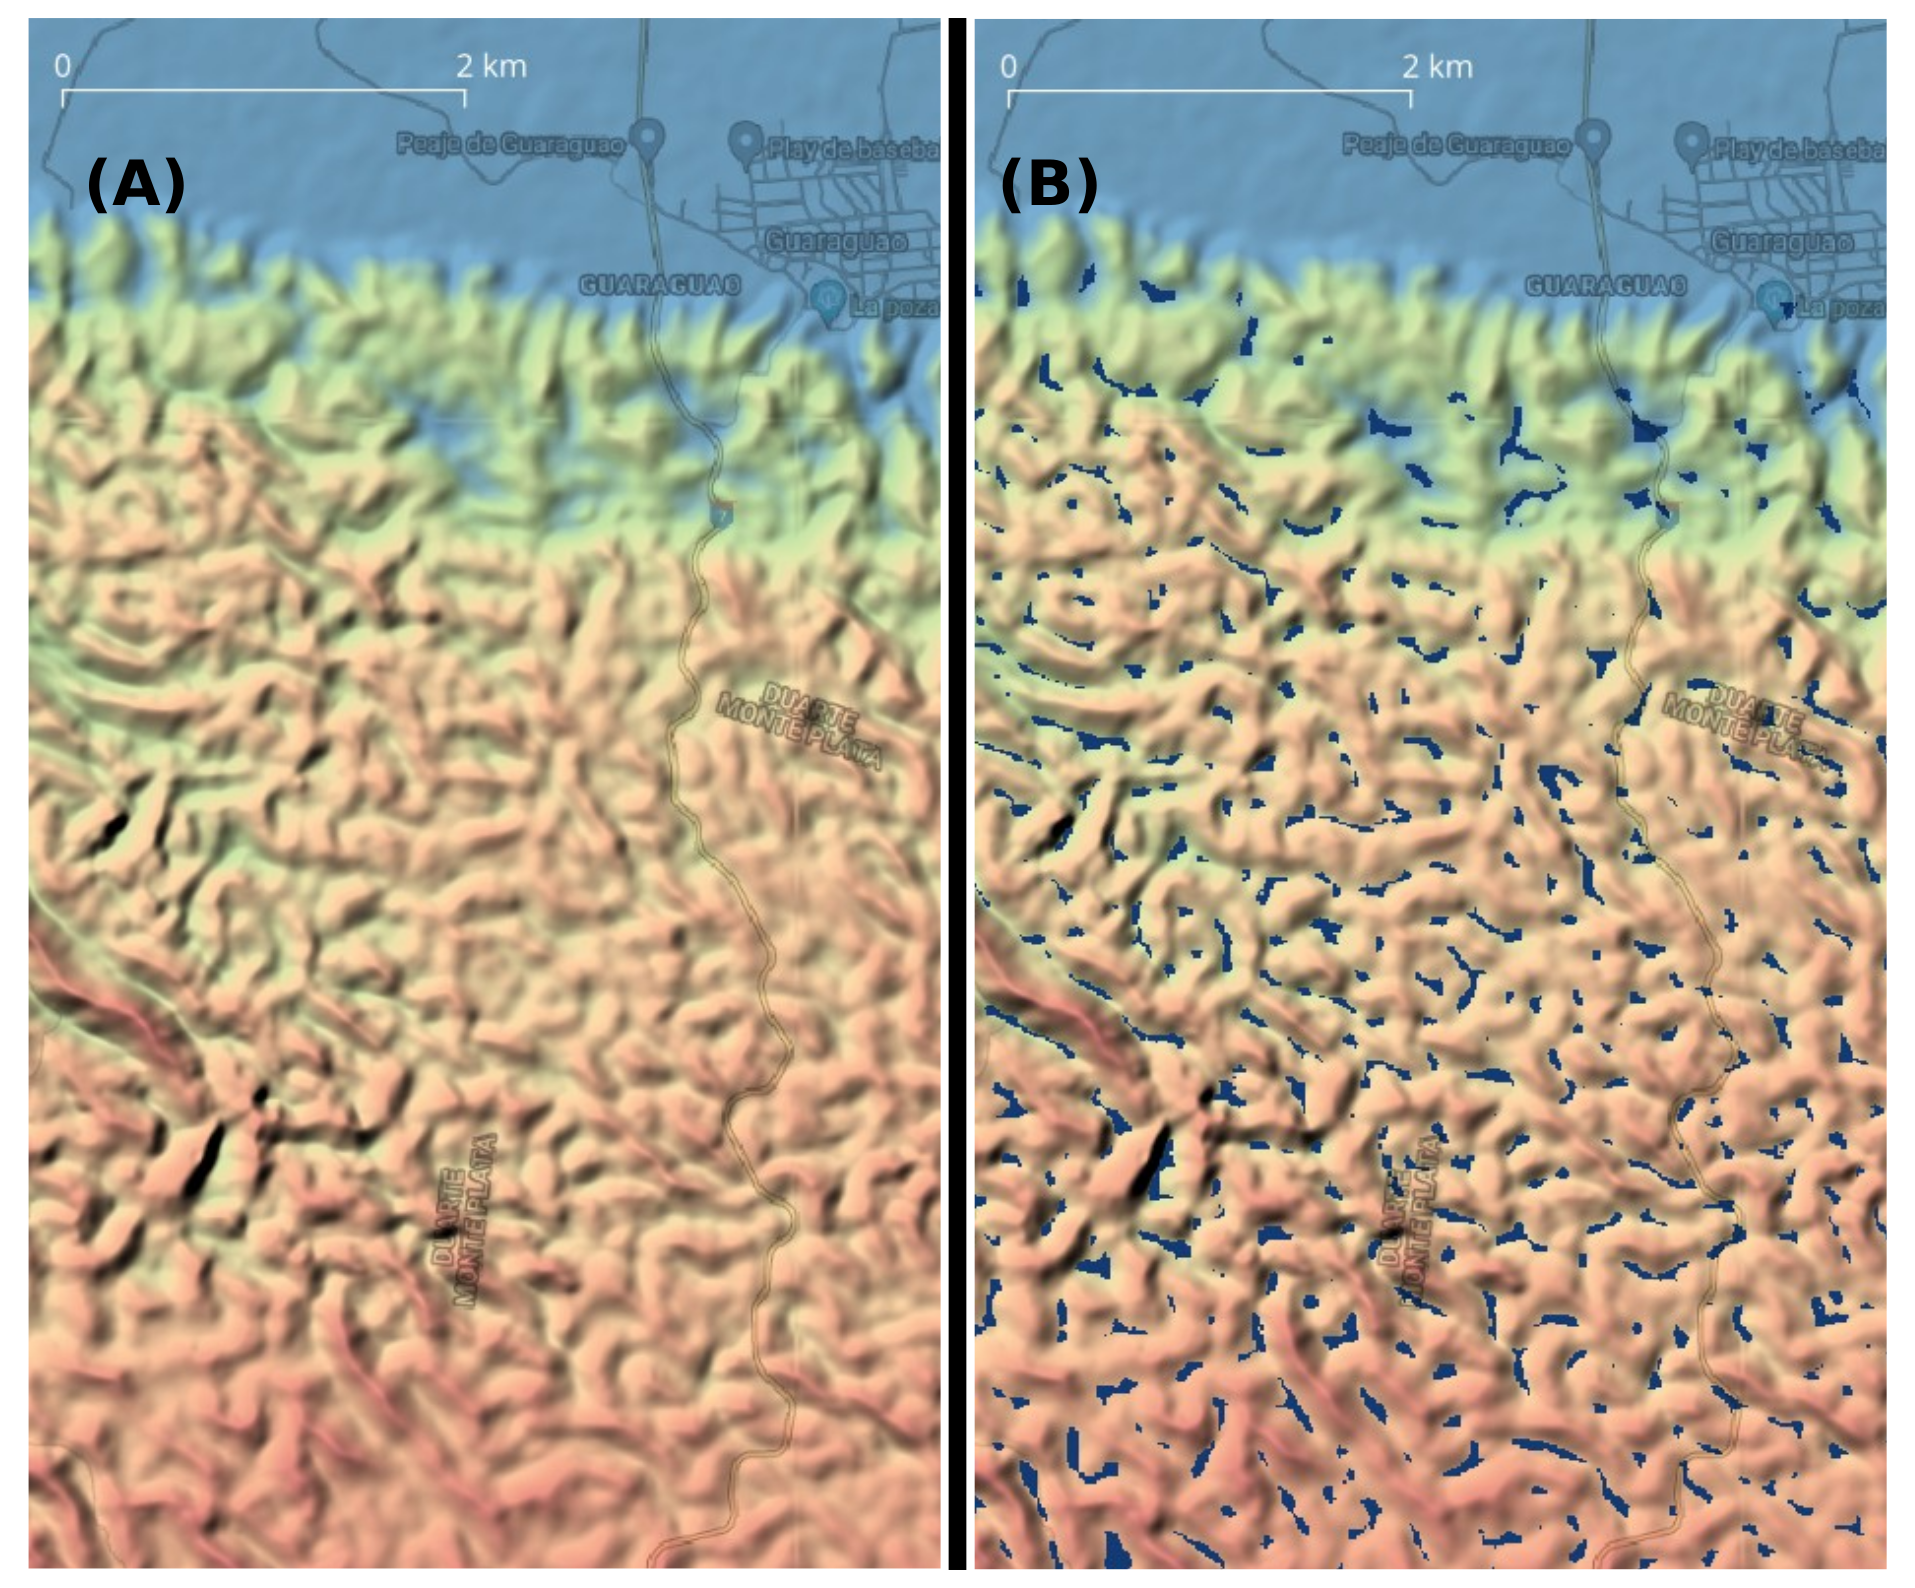
\includegraphics[width=0.8\linewidth]{figuras/depresiones} 

}

\caption{DEM ALOS PALSAR representado como mapa hipsómétrico (rojo y marrón representan terreno elevado, verde y azul claro terreno bajo) sobre relieve sombreado, mostrando el área de Guaraguao, Los Haitises, al sur del río Yuna (nordeste de República Dominicana). (A) sin mostrar depresiones, (B) mostrando depresiones en tonalidad azul oscuro}\label{fig:depresiones}
\end{figure}

\hypertarget{suplemento-meotodoluxf3gico-para-la-subsecciuxf3n-procesamiento-de-hidrologuxeda-computacional}{%
\subsection*{Suplemento meotodológico para la subsección ``Procesamiento
de hidrología
computacional''}\label{suplemento-meotodoluxf3gico-para-la-subsecciuxf3n-procesamiento-de-hidrologuxeda-computacional}}
\addcontentsline{toc}{subsection}{Suplemento meotodológico para la
subsección ``Procesamiento de hidrología computacional''}

Las técnicas de hidrología computacional han experimentado una
considerable transformación desde su origen en el siglo pasado hasta la
actualidad, un proceso evolutivo al que han contribuido múltiples
entidades y personas de manera directa (Ehlschlaeger, 1989; Freeman,
1991; Holmgren, 1994; Larson et~al., 1991; McCool et~al., 1987; Metz
et~al., 2011; Moore et~al., 1991; Quinn et~al., 1991; Weltz et~al.,
1988). De manera particular, en las últimas dos décadas, se han
realizado avances que han expandido el alcance y profundidad de la
hidrología computacional como disciplina, abriendo nuevas fronteras de
conocimiento y posibilitando abordajes más sofisticados y detallados de
los fenómenos hídricos. En este proceso, GRASS GIS ha jugado un papel
fundamental, pues no solo ha mantenido activo calendario de lanzamiento
de versiones, sino que también ha ampliado, gracias a comunidad, el
número de herramientas de forma significativa.

Para realizar análisis de cuencas y redes de drenaje en GRASS GIS, el
complemento por excelencia es \texttt{r.watershed} (GRASS Development
Team, 2022d), el cual ofrece la posibilidad de crear mapas de
acumulación de flujo usando algoritmos avanzados, y facilita también la
tarea de extraer \emph{talwegs} y redes de drenaje, y delimitar cuencas.
Alternativamente, en los casos en los que los que existe especial
interés por el análisis de redes de drenaje y la jerarquía hidrográfica,
se utiliza la familia de complementos \texttt{r.stream*} (Jasiewicz y
Metz, 2011). Dentro de esta familia se encuentran
\texttt{r.stream.extract} para generar la red, \texttt{r.stream.order}
para calcular su jerarquía (requiere de los subproductos generados para
la herramienta anterior), y \texttt{r.stream.basins} para crear cuencas
hidrográficas en función de la jerarquía. En este sentido, debemos
elegir apropiadamente entre \texttt{r.watershed} o la familia
\texttt{r.stream*} según nuestras necesidades y objetivos, o usar ambos
si nos interesan resultados combinados, pero tomando las debidas
precauciones.

Ambos complementos necesitan de dos mapas derivados para generar
productos hidrológicos, los cuales pueden ser generados por ellos
mismos; estos son el mapa de la red propiamente (\texttt{stream\_rast}),
y el de dirección de drenaje (\texttt{direction}). En este sentido, debe
evitarse combinar mapas generados por algoritmos distintos para mantener
la consistencia (por ejemplo, se desaconseja generar
\texttt{stream\_ras} con \texttt{r.watershed} y \texttt{direction} con
\texttt{r.stream*}, y viceversa), por lo que se recomienda generar ambos
mapas por medio del mismo algoritmo.

Considerando que nuestro objetivo principal es la jerarquía de red,
podíamos iniciar con \texttt{r.stream.extract} para generar los insumos
para \texttt{r.stream.order}. Pero dado que este último requiere el mapa
de acumulación flujo, el cual sólo es producido por
\texttt{r.watershed}, generamos primero este mapa. Por lo tanto, sólo
usamos \texttt{r.watershed} para obtener el mapa de acumulación que
necesitamos en la aplicación de la familia \texttt{r.stream.*}.

Previo al inicio de los análisis hidrológicos, aplicamos una máscara
ajustada a la línea de costa y los límites fronterizos del país para
evitar que las redes extraídas se extiendan al mar, y creamos una zona
de influencia en el límite fronterizo para permitir la salida y entrada
de flujo a través de este. Posteriormente, extrajimos el mapa de
acumulación de flujo.

\begin{Shaded}
\begin{Highlighting}[]
\CommentTok{\# Importar máscara}
\ExtensionTok{v.import} \AttributeTok{{-}{-}overwrite}\NormalTok{ input=mascara{-}1km{-}solo{-}en{-}frontera.gpkg }\DataTypeTok{\textbackslash{}}
\NormalTok{  output=mascara\_1km\_solo\_en\_frontera}
\CommentTok{\# Fijar máscara}
\ExtensionTok{r.mask} \AttributeTok{{-}r}
\ExtensionTok{r.mask}\NormalTok{ vector=mascara\_1km\_solo\_en\_frontera}

\CommentTok{\# Acumulación de flujo}
\BuiltInTok{time}\NormalTok{ r.watershed }\AttributeTok{{-}{-}overwrite} \AttributeTok{{-}{-}verbose}\NormalTok{ elevation=dem\_tallado }\DataTypeTok{\textbackslash{}}
\NormalTok{ depression=depresiones\_todas accumulation=rwshed\_acum }\DataTypeTok{\textbackslash{}}
\NormalTok{ threshold=180 stream=rwshed\_talwegs }\DataTypeTok{\textbackslash{}}
\NormalTok{ memory=32000}
\BuiltInTok{echo} \StringTok{"r.watershed finalizado"} \KeywordTok{|} \ExtensionTok{mail} \AttributeTok{{-}s} \StringTok{"Mensaje sobre r.watershed"}\NormalTok{ USUARIO@MAIL}
\CommentTok{\#\# real 10m14.295s}
\CommentTok{\# El umbral 180 se usó en la extracción de una red de muestra, como forma de}
\CommentTok{\# previsualizar una hidrografía inicial, no para generar la red definitiva.}
\CommentTok{\# Dependiendo de la aplicación deseada, otras salidas del addon son:}
\CommentTok{\# drainage=rwshed\_direccion\_drenaje \textbackslash{}}
\CommentTok{\# basin=rwshed\_cuencas \textbackslash{}}
\CommentTok{\# half\_basin=rwshed\_hemicuenca \textbackslash{}}
\CommentTok{\# tci=rwshed\_tci spi=rwshed\_spi \textbackslash{}}
\CommentTok{\# length\_slope=rwshed\_longitud\_vertiente \textbackslash{}}
\CommentTok{\# slope\_steepness=rwshed\_empinamiento \textbackslash{}}
\CommentTok{\# retention=rwshed\_retencion\_flujo \textbackslash{}}
\CommentTok{\# max\_slope\_length=rwshed\_max\_longitud\_vertiente \textbackslash{}}
\end{Highlighting}
\end{Shaded}

\begin{figure}

{\centering \includegraphics[width=0.8\linewidth]{figuras/acumulacion-flujo-y-red-rwshed} 

}

\caption{Mapa de acumulación de flujo generado con `r.watershed`. En cartela, detalle del mapa en la cuenca del río Yaque del Sur.}\label{fig:acumyredrwshed}
\end{figure}

Usando como insumos el DEM y el mapa de acumulación producido por
\texttt{r.watershed}, obtuvimos la red hidrográfica utilizando
\texttt{r.stream.extract}. Esta etapa requirió la evaluación de umbrales
de acumulación óptimos a través de inspección visual. El umbral de
acumulación es un área de debate en hidrología computacional. Nos
enfocamos en la evaluación de criterios para la extracción de
\emph{talwegs} en un sentido amplio, sin considerarlos como cursos
fluviales permanentes. Reconocemos que la determinación de la
permanencia fluvial requeriría un análisis detallado de las
características individuales de cada cuenca, incluyendo aspectos como la
pendiente, tamaño, litología y clima.

Siguiendo las mejores prácticas, realizamos diversas ejecuciones del
complemento \texttt{r.stream.extract} usando varios umbrales para
identificar la red hidrográfica más adecuada en nuestra área de interés
(Freeman, 1991; Jasiewicz y Metz, 2011; Marchesini et~al., 2021). Para
seleccionar un umbral de acumulación óptimo, consideramos cuatro
criterios: consistencia con estudios similares, suficiente densidad de
red, evitar una generalización excesiva de la red, y prevenir una red
demasiado densa que incluya áreas sin características hidrológicas
mínimas. Dado que nuestro DEM tiene una resolución espacial de 12.5 m,
examinamos diferentes umbrales para obtener una red hidrográfica
adecuada. En \texttt{r.stream.extract}, optamos por los umbrales de
acumulación de 180, 540 y 900 celdas, equivalentes a 3, 8 y 14 hectáreas
de superficie, respectivamente. Estos umbrales están en línea con los
utilizados en estudios que consultamos, donde se evaluaron áreas
propensas a inundaciones y cuencas de captación (Freeman, 1991;
Marchesini et~al., 2021).

El código necesario para generar las distintas redes evaluadas lo
implementamos mediante un bucle \texttt{for} en Bash para mayor
eficiencia y consistencia en el procesamiento. Hicimos que el bucle
iterara automáticamente sobre los tres umbrales de acumulación, usando
los valores de umbral como iterador (\texttt{i=\{180..900..360\}}, debe
leerse como ``itera desde 180 a 900 en incrementos de 360 enteros'',
resultando en los valores 180, 540 y 900), el cual pasamos como
argumento del parámetro \texttt{threshold}. Finalmente, para cada red
generada con los distintos umbrales, calculamos la longitud de cursos
fluviales, actualizamos la base de datos de GRASS GIS y generamos un
archivo de texto resumen que posteriormente importamos a R para obtener
estadísticos básicos.

\begin{Shaded}
\begin{Highlighting}[]
\CommentTok{\# Extraer redes de drenaje para tres umbrales de acumulación distintos}
\CommentTok{\# En bucle}
\ControlFlowTok{for}\NormalTok{ i }\KeywordTok{in} \KeywordTok{\textasciigrave{}}\BuiltInTok{echo} \DataTypeTok{\{}\DecValTok{180}\DataTypeTok{..}\DecValTok{900}\DataTypeTok{..}\DecValTok{360}\DataTypeTok{\}}\KeywordTok{\textasciigrave{};} \DataTypeTok{\textbackslash{}}
  \ControlFlowTok{do} \BuiltInTok{echo} \AttributeTok{{-}e} \StringTok{"\textbackslash{}nTRABAJANDO EL UMBRAL DE ACUMULACIÓN }\VariableTok{$i}\StringTok{ ...\textbackslash{}n"}\KeywordTok{;} \DataTypeTok{\textbackslash{}}
  \BuiltInTok{time}\NormalTok{ r.stream.extract }\AttributeTok{{-}{-}overwrite}\NormalTok{ elevation=dem\_tallado accumulation=rwshed\_acum }\DataTypeTok{\textbackslash{}}
\NormalTok{    depression=depresiones\_todas threshold=}\VariableTok{$i} \DataTypeTok{\textbackslash{}}
\NormalTok{    stream\_vector=rstream\_talwegs\_umbral\_}\VariableTok{$i}\NormalTok{ stream\_raster=rstream\_talwegs\_umbral\_}\VariableTok{$i} \DataTypeTok{\textbackslash{}}
\NormalTok{    direction=rstream\_direccion\_umbral\_}\VariableTok{$i}\NormalTok{ memory=32000}\KeywordTok{;} \DataTypeTok{\textbackslash{}}
  \BuiltInTok{echo} \AttributeTok{{-}e} \StringTok{"r.stream.extract umbral }\VariableTok{$i}\StringTok{ finalizado"} \KeywordTok{|}\DataTypeTok{\textbackslash{}}
    \ExtensionTok{mail} \AttributeTok{{-}s} \StringTok{"Mensaje sobre r.stream.extract"}\NormalTok{ USUARIO@MAIL}\KeywordTok{;} \DataTypeTok{\textbackslash{}}
\ControlFlowTok{done}
\CommentTok{\#\# real 11m28.455s}
\CommentTok{\#\# real 11m26.908s}
\CommentTok{\#\# real 11m30.074s}
\CommentTok{\# Único umbral, para testing}
\CommentTok{\# time r.stream.extract {-}{-}overwrite elevation=dem\_tallado accumulation=rwshed\_acum \textbackslash{}}
\CommentTok{\#   depression=depresiones\_todas threshold=64 \textbackslash{}}
\CommentTok{\#   stream\_vector=rstream\_talwegs\_umbral\_64 stream\_raster=rstream\_talwegs\_umbral\_64 \textbackslash{}}
\CommentTok{\#     direction=rstream\_direccion\_umbral\_64 memory=32000}
\CommentTok{\# echo "Job finished" | mail {-}s "Job finished" USUARIO@MAIL}
\CommentTok{\#\# real 11m46.930s}
\CommentTok{\# Calcular estadisticos, y pasar a archivo}
\ControlFlowTok{for}\NormalTok{ i }\KeywordTok{in} \KeywordTok{\textasciigrave{}}\BuiltInTok{echo} \DataTypeTok{\{}\DecValTok{180}\DataTypeTok{..}\DecValTok{900}\DataTypeTok{..}\DecValTok{360}\DataTypeTok{\}}\KeywordTok{\textasciigrave{};} \DataTypeTok{\textbackslash{}}
  \ControlFlowTok{do} \ExtensionTok{v.to.db} \AttributeTok{{-}p}\NormalTok{ option=length map=rstream\_talwegs\_umbral\_}\VariableTok{$i} \OperatorTok{\textgreater{}}\DataTypeTok{\textbackslash{}}
\NormalTok{    stats\_length\_rstream\_talwegs\_umbral\_}\VariableTok{$i}\NormalTok{.txt}\KeywordTok{;}
\ControlFlowTok{done}
\end{Highlighting}
\end{Shaded}

\begin{Shaded}
\begin{Highlighting}[]
\NormalTok{stats\_rstream\_talwegs }\OtherTok{\textless{}{-}} \FunctionTok{sapply}\NormalTok{(}\FunctionTok{as.character}\NormalTok{(}\FunctionTok{c}\NormalTok{(}\DecValTok{180}\NormalTok{, }\DecValTok{540}\NormalTok{, }\DecValTok{900}\NormalTok{)), }\ControlFlowTok{function}\NormalTok{(x) }
  \FunctionTok{read\_delim}\NormalTok{(}\FunctionTok{paste0}\NormalTok{(dem\_proc\_dir, }\StringTok{\textquotesingle{}/\textquotesingle{}}\NormalTok{, }\StringTok{\textquotesingle{}stats\_length\_rstream\_talwegs\_umbral\_\textquotesingle{}}\NormalTok{, x, }\StringTok{\textquotesingle{}.txt\textquotesingle{}}\NormalTok{),}
             \AttributeTok{progress =}\NormalTok{ F, }\AttributeTok{show\_col\_types =}\NormalTok{ F), }\AttributeTok{simplify =}\NormalTok{ F)}
\NormalTok{n\_rstream\_talwegs }\OtherTok{\textless{}{-}}\NormalTok{ stats\_rstream\_talwegs }\SpecialCharTok{\%\textgreater{}\%} 
  \FunctionTok{map}\NormalTok{(}\SpecialCharTok{\textasciitilde{}}\NormalTok{ .x }\SpecialCharTok{\%\textgreater{}\%} \FunctionTok{filter}\NormalTok{(}\SpecialCharTok{!}\NormalTok{cat}\SpecialCharTok{=={-}}\DecValTok{1}\NormalTok{) }\SpecialCharTok{\%\textgreater{}\%}\NormalTok{ nrow) }\SpecialCharTok{\%\textgreater{}\%}\NormalTok{ unlist}
\NormalTok{length\_rstream\_talwegs }\OtherTok{\textless{}{-}}\NormalTok{ stats\_rstream\_talwegs }\SpecialCharTok{\%\textgreater{}\%}
  \FunctionTok{map}\NormalTok{(}\SpecialCharTok{\textasciitilde{}}\NormalTok{ .x }\SpecialCharTok{\%\textgreater{}\%} \FunctionTok{filter}\NormalTok{(}\SpecialCharTok{!}\NormalTok{cat}\SpecialCharTok{=={-}}\DecValTok{1}\NormalTok{) }\SpecialCharTok{\%\textgreater{}\%} \FunctionTok{pull}\NormalTok{(length) }\SpecialCharTok{\%\textgreater{}\%}\NormalTok{ sum}\SpecialCharTok{/}\DecValTok{1000}\NormalTok{) }\SpecialCharTok{\%\textgreater{}\%}\NormalTok{ unlist}
\end{Highlighting}
\end{Shaded}

Evaluamos los resultados y recopilamos los estadísticos esenciales de
cada red formada con los distintos umbrales. Para los umbrales de 180,
540 y 900 celdas, se obtuvieron \textbf{420010, 192566 y 130278
segmentos} correspondientemente, acumulando \textbf{138476, 98203 y
82054 kilómetros} de longitud en cada caso (estos valores excluyen una
pequeña fracción del total fuera de la máscara). Para cada una de las
redes, evaluamos el grado de alineación con nuestros criterios de
selección de la red óptima, tras lo cual elegimos la red generada con el
umbral de acumulación de 540 celdas. Sin embargo, mantuvimos las
restantes en la base de datos y les aplicamos todos los subsiguientes
algoritmos de análisis de hidrología computacional, hasta alcanzar los
resultados finales.

\begin{figure}

{\centering \includegraphics[width=0.8\linewidth]{figuras/red-indiferenciada} 

}

\caption{Red de drenaje extraída para tres umbrales de acumulación: (A) 180 celdas, equivalente a ~3 ha; (B) 540 celdas, equivalente a ~8 ha; (C) 900 celdas, equivalente a ~14 ha. La imagen de fondo es un relieve sombreado a partir de DEM ALOS PALSAR, mostrando el área de El Arroyazo en la reserva científica Ébano Verde (provincia La Vega, cordillera Central de República Dominicana)}\label{fig:redindiferenciada}
\end{figure}

Posteriormente, calculamos el orden jerárquico de la red hidrográfica,
proceso que repetimos para cada uno de los umbrales de acumulación que
definimos previamente, es decir, 180, 540 y 900 celdas. Al igual que en
casos anteriores, utilizamos un bucle en Bash para iterar
automáticamente sobre los tres umbrales de acumulación; en este caso,
los valores del índice se correspondían con los sufijos de los mapas de
entrada (\texttt{\_\$i}). El núcleo del bucle, en este caso, contiene la
ejecución del complemento \texttt{r.stream.order} de GRASS GIS. Este
complemento se invoca con una serie de argumentos que especifican los
mapas de entrada y salida que se deben usar en el cálculo. De manera
específica, le proporcionamos el mapa de \emph{talwegs} o cursos
(parámetro \texttt{stream\_rast}), el mapa de dirección de drenaje
(\texttt{direction}), el mapa de elevación (\texttt{elevation}), y el
mapa de acumulación (\texttt{accumulation}), todos correspondientes al
umbral de acumulación que está siendo procesado en cada iteración.
Adicionalmente, especificamos los nombres de los mapas de salida que
contienen el orden de red según los métodos de Strahler y Horton
(argumentos \texttt{strahler} y \texttt{horton}) (Horton, 1945;
Strahler, 1957), así como el mapa de topología (\texttt{topo}) y el
vectorial de salida (\texttt{stream\_vect}).

\begin{Shaded}
\begin{Highlighting}[]
\CommentTok{\# Extraer orden de red en bucle}
\ControlFlowTok{for}\NormalTok{ i }\KeywordTok{in} \KeywordTok{\textasciigrave{}}\BuiltInTok{echo} \DataTypeTok{\{}\DecValTok{180}\DataTypeTok{..}\DecValTok{900}\DataTypeTok{..}\DecValTok{360}\DataTypeTok{\}}\KeywordTok{\textasciigrave{};} \DataTypeTok{\textbackslash{}}
  \ControlFlowTok{do} \BuiltInTok{echo} \AttributeTok{{-}e} \StringTok{"\textbackslash{}nTRABAJANDO EL UMBRAL DE ACUMULACIÓN }\VariableTok{$i}\StringTok{ ...\textbackslash{}n"}\KeywordTok{;} \DataTypeTok{\textbackslash{}}
  \BuiltInTok{time}\NormalTok{ r.stream.order }\AttributeTok{{-}{-}overwrite}\NormalTok{ stream\_rast=rstream\_talwegs\_umbral\_}\VariableTok{$i} \DataTypeTok{\textbackslash{}}
\NormalTok{    direction=rstream\_direccion\_umbral\_}\VariableTok{$i} \DataTypeTok{\textbackslash{}}
\NormalTok{    elevation=dem\_tallado accumulation=rwshed\_acum }\DataTypeTok{\textbackslash{}}
\NormalTok{    stream\_vect=rstream\_orden\_de\_red\_umbral\_}\VariableTok{$i} \DataTypeTok{\textbackslash{}}
\NormalTok{    strahler=rstream\_orden\_strahler\_de\_red\_umbral\_}\VariableTok{$i} \DataTypeTok{\textbackslash{}}
\NormalTok{    horton=rstream\_orden\_horton\_de\_red\_umbral\_}\VariableTok{$i} \DataTypeTok{\textbackslash{}}
\NormalTok{    topo=topologia\_orden\_umbral\_}\VariableTok{$i}\NormalTok{ memory=32000}\KeywordTok{;} \DataTypeTok{\textbackslash{}}
  \BuiltInTok{echo} \AttributeTok{{-}e} \StringTok{"r.stream.order umbral de acumulación }\VariableTok{$i}\StringTok{ finalizado"} \KeywordTok{|}\DataTypeTok{\textbackslash{}}
    \ExtensionTok{mail} \AttributeTok{{-}s} \StringTok{"Mensaje sobre r.stream.order"}\NormalTok{ USUARIO@MAIL}\KeywordTok{;} \DataTypeTok{\textbackslash{}}
\ControlFlowTok{done}
\CommentTok{\#\# real 1m34.983s}
\CommentTok{\#\# real 1m18.662s}
\CommentTok{\#\# real 1m14.986s}
\CommentTok{\# Aplicación de algoritmo con un único umbral, sólo para pruebas}
\CommentTok{\# time r.stream.order {-}{-}overwrite \textbackslash{}}
\CommentTok{\#     stream\_rast=rstream\_talwegs direction=rstream\_direccion \textbackslash{}}
\CommentTok{\#     elevation=dem\_tallado accumulation=rwshed\_acum stream\_vect=order\_todos \textbackslash{}}
\CommentTok{\#     topo=topologia\_orden memory=32000}
\CommentTok{\# echo "Job finished" | mail {-}s "Job finished" USUARIO@MAIL}
\end{Highlighting}
\end{Shaded}

\begin{figure}

{\centering \includegraphics[width=0.8\linewidth]{figuras/red-orden} 

}

\caption{Orden de red de Strahler para redes de drenaje generadas a partir de tres umbrales de acumulación: (A) 180 celdas, equivalente a ~3 ha; (B) 540 celdas, equivalente a ~8 ha; (C) 900 celdas, equivalente a ~14 ha. El área mostrada corresponde al río San Juan, afluente del río Yaque del Sur (vertiente sur de la cordillera Central de República Dominicana)}\label{fig:redorden3umbrales}
\end{figure}

\begin{figure}

{\centering 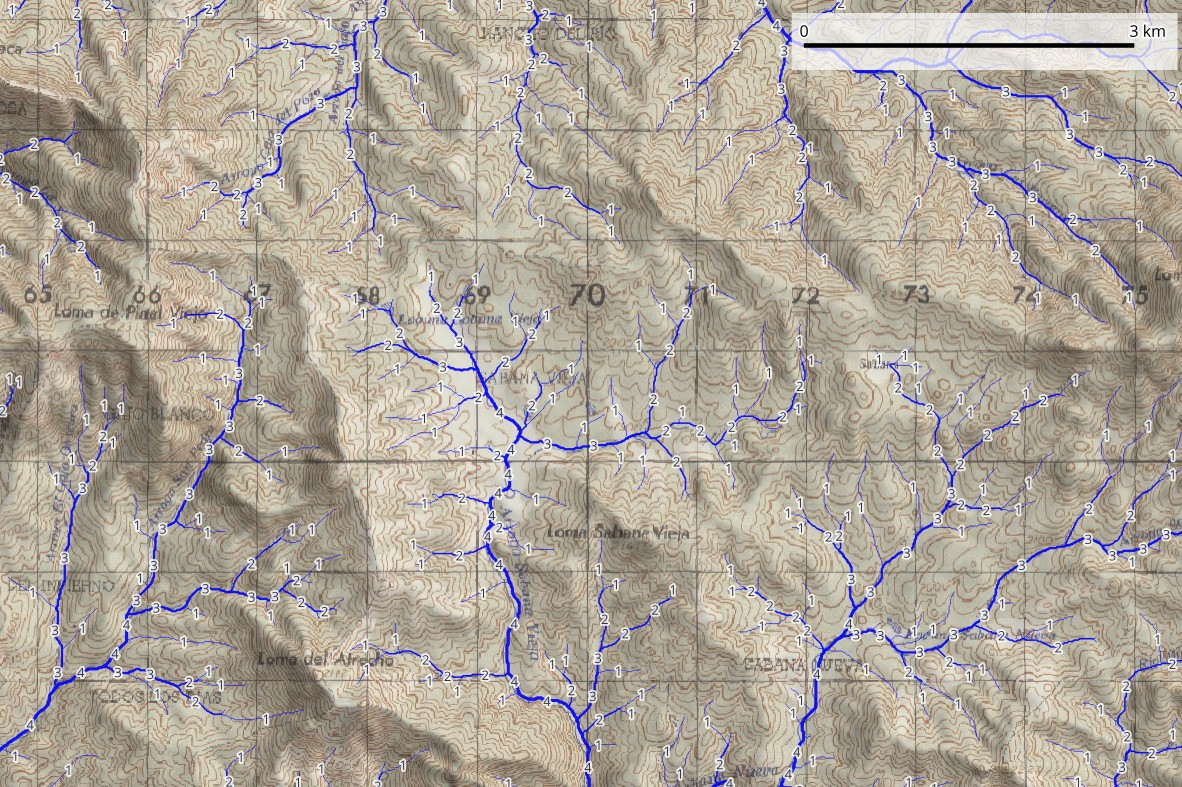
\includegraphics[width=0.8\linewidth]{figuras/red-orden-detalle-mtn} 

}

\caption{Orden de red de Strahler en el área del pico de la Viuda y Sabana Vieja, provincia San Juan (vertiente sur de la cordillera Central de República Dominicana). Esta red fue generada usando un umbral de acumulación de 180 celdas, equivalente a ~3 ha. De fondo, mapa topográfico nacional escala 1:50,000 y relieve sombreado}\label{fig:redordenumbral180}
\end{figure}

Corregimos la topología con \texttt{v.clean}, pero sólo para la red
generada con el umbral de acumulación de 540 celdas. Eliminamos los
cursos con longitud 0 metros y actualizamos la longitud de cada curso en
el campo \texttt{length} usando el complemento \texttt{v.to.db}.

\begin{Shaded}
\begin{Highlighting}[]
\ExtensionTok{v.clean} \AttributeTok{{-}{-}overwrite}\NormalTok{ layer=1 }\DataTypeTok{\textbackslash{}}
\NormalTok{  input=rstream\_orden\_de\_red\_umbral\_540 }\DataTypeTok{\textbackslash{}}
\NormalTok{  output=rstream\_orden\_de\_red\_umbral\_540\_cleaned }\DataTypeTok{\textbackslash{}}
\NormalTok{  tool=rmline}
\ExtensionTok{v.to.db} \AttributeTok{{-}{-}overwrite}\NormalTok{ option=length type=line columns=area }\DataTypeTok{\textbackslash{}}
\NormalTok{  map=rstream\_orden\_de\_red\_umbral\_540\_cleaned}
\end{Highlighting}
\end{Shaded}

Para completar la caracterización de las redes de drenaje, empleamos dos
enfoques distintos: exploración visual y análisis estadístico. Para la
exploración visual, usamos el mapa de la red y lo desplegamos en QGIS.
Para la obtención de resultados analíticos, usamos el addon
\texttt{r.stream.stats}, con el que calculamos los estadísticos de las
redes jerarquizadas---longitud de tramos, área drenada, pendientes,
razón de bifurcación----creadas con el addon \texttt{r.stream.order}.
Mostramos a continuación las instrucciones necesarias para obtener los
estadísticos mediante \texttt{r.stream.stats} El archivo de texto
resultante lo utilizamos en los análisis estadísticos posteriores en una
sesión de \texttt{R}.

\begin{Shaded}
\begin{Highlighting}[]
\CommentTok{\# Salida resumen}
\ExtensionTok{r.stream.stats} \AttributeTok{{-}{-}overwrite} \AttributeTok{{-}o} \DataTypeTok{\textbackslash{}}
\NormalTok{  stream\_rast=rstream\_orden\_strahler\_de\_red\_umbral\_540 }\DataTypeTok{\textbackslash{}}
\NormalTok{  direction=rstream\_direccion\_umbral\_540 }\DataTypeTok{\textbackslash{}}
\NormalTok{  elevation=dem\_pseudo\_ortometrico }\DataTypeTok{\textbackslash{}}
\NormalTok{  output=stats\_rstream\_order\_strahler\_red\_umbral\_540\_horton.txt }\DataTypeTok{\textbackslash{}}
\NormalTok{  memory=32000}
\CommentTok{\# Salida desagregada}
\ExtensionTok{r.stream.stats} \AttributeTok{{-}{-}overwrite} \DataTypeTok{\textbackslash{}}
\NormalTok{  stream\_rast=rstream\_orden\_strahler\_de\_red\_umbral\_540 }\DataTypeTok{\textbackslash{}}
\NormalTok{  direction=rstream\_direccion\_umbral\_540 }\DataTypeTok{\textbackslash{}}
\NormalTok{  elevation=dem\_pseudo\_ortometrico }\DataTypeTok{\textbackslash{}}
\NormalTok{  output=stats\_rstream\_order\_strahler\_red\_umbral\_540.txt }\DataTypeTok{\textbackslash{}}
\NormalTok{  memory=32000}
\end{Highlighting}
\end{Shaded}

A continuación, delimitamos cuencas y subcuencas según la jerarquía de
red, con independencia de si tratara de cuencas tributarias o no, para
lo cual usamos el complemento \texttt{r.stream.basins} especificando la
opción (\emph{flag}) \texttt{-c}, que utiliza una secuencia única de
categorías (en nuestro caso, órdenes) para delimitar las cuencas en
lugar de flujos de entrada. En este caso, construimos un bucle
\texttt{for} doble, anidando el orden de red dentro del umbral de
acumulación. Así, para cada uno de los mapas de redes hidrográficas
según los tres umbrales de acumulación, delimitamos las cuencas de cada
uno de los órdenes de Strahler disponibles. Al utilizar el criterio
orden de red, las unidades delimitadas por este procedimiento incluyen
tanto cuencas completas como subcuencas (tributarias), por lo que la
mayoría contiene redes de drenaje tributarias (ríos que desembocan en
otros ríos).

\begin{Shaded}
\begin{Highlighting}[]
\CommentTok{\# Delimitar cuencas según jerarquía}
\CommentTok{\# En bucle}
\BuiltInTok{time}\NormalTok{ for i in }\KeywordTok{\textasciigrave{}}\BuiltInTok{echo} \DataTypeTok{\{}\DecValTok{180}\DataTypeTok{..}\DecValTok{900}\DataTypeTok{..}\DecValTok{360}\DataTypeTok{\}}\KeywordTok{\textasciigrave{};} \DataTypeTok{\textbackslash{}}
  \ControlFlowTok{do} \ControlFlowTok{for}\NormalTok{ j }\KeywordTok{in} \KeywordTok{\textasciigrave{}}\BuiltInTok{echo} \DataTypeTok{\{}\DecValTok{1}\DataTypeTok{..}\DecValTok{8}\DataTypeTok{..}\DecValTok{1}\DataTypeTok{\}}\KeywordTok{\textasciigrave{};} \DataTypeTok{\textbackslash{}}
    \ControlFlowTok{do} \BuiltInTok{echo} \AttributeTok{{-}e} \StringTok{"\textbackslash{}nTRABAJANDO EL UMBRAL DE ACUMULACIÓN }\VariableTok{$i}\StringTok{, orden }\VariableTok{$j}\StringTok{...\textbackslash{}n"}\KeywordTok{;} \DataTypeTok{\textbackslash{}}
    \ExtensionTok{r.stream.basins} \AttributeTok{{-}c} \AttributeTok{{-}{-}overwrite}\NormalTok{ direction=rstream\_direccion\_umbral\_}\VariableTok{$i} \DataTypeTok{\textbackslash{}}
\NormalTok{      stream\_rast=rstream\_orden\_strahler\_de\_red\_umbral\_}\VariableTok{$i}\NormalTok{ cats=}\VariableTok{$j} \DataTypeTok{\textbackslash{}}
\NormalTok{      basins=rstream\_cuencas\_strahler\_umbral\_}\VariableTok{$\{i\}}\NormalTok{\_orden\_}\VariableTok{$j}\NormalTok{ memory=32000}\KeywordTok{;} \DataTypeTok{\textbackslash{}}
  \ControlFlowTok{done}\KeywordTok{;} \DataTypeTok{\textbackslash{}}
  \BuiltInTok{echo} \AttributeTok{{-}e} \StringTok{"r.stream.basins umbral de acumulación }\VariableTok{$i}\StringTok{ finalizado"} \KeywordTok{|}\DataTypeTok{\textbackslash{}}
    \ExtensionTok{mail} \AttributeTok{{-}s} \StringTok{"Mensaje sobre r.stream.basins"}\NormalTok{ USUARIO@MAIL}\KeywordTok{;} \DataTypeTok{\textbackslash{}}
\ControlFlowTok{done}
\CommentTok{\#\# real 17m42.238s}
\end{Highlighting}
\end{Shaded}

Posteriormente, delimitamos las cuencas con desembocadura en mares,
lagos, lagunas o en pérdidas kársticas. En esta sección aplicamos el
mismo complemento que en el paso anterior (\texttt{r.stream.basins}) en
bucle doble anidado, pero en esta ocasión especificamos la opción
\texttt{-l}. Es decir, delimitamos las cuencas completas, cuya red
desemboca en el mar (exorreicas), o en lagos, lagunas y pérdidas del
karst (endorreicas), y excluimos las subcuencas de redes tributarias
(eg. red cuyo curso principal desemboca en otro río). Por lo tanto, se
trata de cuencas propiamente en la acepción más formal del término, que
significa que no existe---o no se conoce ni se puede detectar con
información disponible---prolongación del drenaje superficial fuera de
ellas.

\begin{Shaded}
\begin{Highlighting}[]
\CommentTok{\# Delimitar cuencas terminales}
\CommentTok{\# En bucle}
\BuiltInTok{time}\NormalTok{ for i in }\KeywordTok{\textasciigrave{}}\BuiltInTok{echo} \DataTypeTok{\{}\DecValTok{180}\DataTypeTok{..}\DecValTok{900}\DataTypeTok{..}\DecValTok{360}\DataTypeTok{\}}\KeywordTok{\textasciigrave{};} \DataTypeTok{\textbackslash{}}
  \ControlFlowTok{do} \ControlFlowTok{for}\NormalTok{ j }\KeywordTok{in} \KeywordTok{\textasciigrave{}}\BuiltInTok{echo} \DataTypeTok{\{}\DecValTok{1}\DataTypeTok{..}\DecValTok{8}\DataTypeTok{..}\DecValTok{1}\DataTypeTok{\}}\KeywordTok{\textasciigrave{};} \DataTypeTok{\textbackslash{}}
    \ControlFlowTok{do} \BuiltInTok{echo} \AttributeTok{{-}e} \StringTok{"\textbackslash{}nTRABAJANDO EL UMBRAL DE ACUMULACIÓN }\VariableTok{$i}\StringTok{, orden }\VariableTok{$j}\StringTok{...\textbackslash{}n"}\KeywordTok{;} \DataTypeTok{\textbackslash{}}
    \ExtensionTok{r.stream.basins} \AttributeTok{{-}lc} \AttributeTok{{-}{-}overwrite}\NormalTok{ direction=rstream\_direccion\_umbral\_}\VariableTok{$i} \DataTypeTok{\textbackslash{}}
\NormalTok{      stream\_rast=rstream\_orden\_strahler\_de\_red\_umbral\_}\VariableTok{$i}\NormalTok{ cats=}\VariableTok{$j} \DataTypeTok{\textbackslash{}}
\NormalTok{      basins=rstream\_cuencas\_strahler\_terminal\_umbral\_}\VariableTok{$\{i\}}\NormalTok{\_orden\_}\VariableTok{$j}\NormalTok{ memory=32000}\KeywordTok{;} \DataTypeTok{\textbackslash{}}
  \ControlFlowTok{done}\KeywordTok{;} \DataTypeTok{\textbackslash{}}
  \BuiltInTok{echo} \AttributeTok{{-}e} \StringTok{"r.stream.basins umbral de acumulación }\VariableTok{$i}\StringTok{ finalizado"} \KeywordTok{|}\DataTypeTok{\textbackslash{}}
    \ExtensionTok{mail} \AttributeTok{{-}s} \StringTok{"Mensaje sobre r.stream.basins"}\NormalTok{ USUARIO@MAIL}\KeywordTok{;} \DataTypeTok{\textbackslash{}}
\ControlFlowTok{done}
\CommentTok{\#\# real 16m16.808s}
\end{Highlighting}
\end{Shaded}

Como último paso en la producción de resultados, convertimos las cuencas
a modelo de datos vectorial, pero para evitar agrandar la base de datos
innecesariamente, elegimos sólo las cuencas generadas para el umbral de
540 celdas. Los vectoriales resultantes nos permitieron un mejor manejo
de los datos para análisis y representación de la cuencas. Describimos
el procedimiento detallado a continuación.

Comenzamos la vectorización ejecutando un bucle para convertir cada capa
ráster de cuencas terminales correspondiente a cada orden de red (desde
1 a 8) en un mapa vectorial de tipo área. Para realizar esta conversión,
utilizamos el complemento \texttt{r.to.vect} de GRASS GIS, añadiendo
también una nueva columna llamada \texttt{strahler} a la tabla de
atributos de cada capa vectorial, que luego actualizamos con el valor
del orden de red Strahler correspondiente. Después de procesar las
cuencas de cada orden, fusionamos todas las capas vectoriales en una
sola utilizando el complemento \texttt{v.patch}. Esto produjo una única
capa vectorial conteniendo información sobre todas las cuencas
terminales para todos los órdenes Strahler. Es importante aclarar que
sólo fueron propiamente clasificadas como polígonos con de orden de red,
aquellas las áreas del ráster que contaban con categorías asignadas
(e.g.~píxeles con valor 1 a 8), es decir, aquellas a las que el
algoritmo \texttt{r.stream.basins} asignó un orden de red debidamente.
Las áreas que formaban el fondo (e.g.~píxeles con valor cero), que
corresponden a espacios con drenaje hacia depresiones sin pertenencia a
jerarquía alguna, conforman la capa ``0'' del mapa vectorial generado
(\texttt{rstream\_cuencas\_strahler\_terminal\_umbral\_540\_todos\_cleaned\ 0}).
Por esta razón, el mapa vectorial de cuencas generado, presenta espacios
vacíos; si hiciera falta recuperar dichos espacios, bastaría con cargar
la referida capa ``0'', tomando en consideración que sus elementos no
cuentan con atributos aprovechables.

Luego, limpiamos y preparamos los datos para el análisis. Primero,
corregimos la topología y actualizamos el área de cada cuenca usando el
complemento \texttt{v.clean}. Eliminamos las áreas inferiores a
4000~m\textsuperscript{2} (cuencas espurias) para mejorar la calidad de
los datos. Posteriormente, eliminamos los registros con un valor de área
nulo (artefactos). Estas etapas de limpieza y preparación son críticas
para garantizar la precisión y relevancia de nuestros resultados.

Finalmente, seleccionamos las filas válidas---las que tenían un valor de
categoría distinto de -1---de la tabla de atributos de nuestra capa
vectorial final, y exportamos estos datos a un archivo de texto. Este
archivo de texto contiene estadísticas del área para cada cuenca
terminal según orden Strahler, lo cual nos proporcionó información
valiosa para nuestro análisis posterior.

\begin{Shaded}
\begin{Highlighting}[]
\CommentTok{\# Cuencas y subcuencas según orden}
\BuiltInTok{time}\NormalTok{ for i in }\KeywordTok{\textasciigrave{}}\BuiltInTok{echo} \DataTypeTok{\{}\DecValTok{1}\DataTypeTok{..}\DecValTok{8}\DataTypeTok{..}\DecValTok{1}\DataTypeTok{\}}\KeywordTok{\textasciigrave{};} \DataTypeTok{\textbackslash{}}
  \ControlFlowTok{do} \BuiltInTok{echo} \AttributeTok{{-}e} \StringTok{"\textbackslash{}nTRABAJANDO EL ORDEN }\VariableTok{$i}\StringTok{...\textbackslash{}n"}\KeywordTok{;} \DataTypeTok{\textbackslash{}}
    \ExtensionTok{r.to.vect} \AttributeTok{{-}{-}overwrite}\NormalTok{ input=rstream\_cuencas\_strahler\_umbral\_540\_orden\_}\VariableTok{$i} \DataTypeTok{\textbackslash{}}
\NormalTok{      output=rstream\_cuencas\_strahler\_umbral\_540\_orden\_}\VariableTok{$i}\NormalTok{ type=area}\KeywordTok{;} \DataTypeTok{\textbackslash{}}
    \ExtensionTok{v.db.addcolumn}\NormalTok{ rstream\_cuencas\_strahler\_umbral\_540\_orden\_}\VariableTok{$i} \DataTypeTok{\textbackslash{}}
\NormalTok{      columns=}\StringTok{"strahler int"}\KeywordTok{;} \DataTypeTok{\textbackslash{}}
    \ExtensionTok{v.db.update}\NormalTok{ rstream\_cuencas\_strahler\_umbral\_540\_orden\_}\VariableTok{$i} \DataTypeTok{\textbackslash{}}
\NormalTok{      col=strahler value=}\VariableTok{$i}\NormalTok{ where=}\StringTok{"strahler IS NULL"}\KeywordTok{;} \DataTypeTok{\textbackslash{}}
    \CommentTok{\# Calcular estadisticos, y pasar a archivo}
    \CommentTok{\#\# Preparación de fuentes (corrección de topología \textgreater{}}
    \CommentTok{\#\#                         actualización de área \textgreater{}}
    \CommentTok{\#\#                         eliminar registros)}
    \ExtensionTok{v.clean} \AttributeTok{{-}{-}overwrite}\NormalTok{ layer=1 }\DataTypeTok{\textbackslash{}}
\NormalTok{      input=rstream\_cuencas\_strahler\_umbral\_540\_orden\_}\VariableTok{$i} \DataTypeTok{\textbackslash{}}
\NormalTok{      output=foo }\DataTypeTok{\textbackslash{}}
\NormalTok{      tool=rmarea threshold=4000}
    \ExtensionTok{v.to.db} \AttributeTok{{-}{-}overwrite}\NormalTok{ option=area type=centroid columns=area }\DataTypeTok{\textbackslash{}}
\NormalTok{      map=foo}
    \ExtensionTok{v.db.droprow} \AttributeTok{{-}{-}overwrite} \DataTypeTok{\textbackslash{}}
\NormalTok{      input=foo }\DataTypeTok{\textbackslash{}}
\NormalTok{      output=rstream\_cuencas\_strahler\_umbral\_540\_orden\_}\VariableTok{$i}\NormalTok{ where=}\StringTok{"area IS NULL"}
    \ExtensionTok{g.remove} \AttributeTok{{-}f}\NormalTok{ type=vector }\DataTypeTok{\textbackslash{}}
\NormalTok{    name=foo}
\ControlFlowTok{done}
\CommentTok{\#\# real 19m7.443s}


\CommentTok{\# Limpiando las cuencas de órdenes 2 y 3 de menos de 60,000 m2}
\ControlFlowTok{for}\NormalTok{ i }\KeywordTok{in} \KeywordTok{\textasciigrave{}}\BuiltInTok{echo} \DataTypeTok{\{}\DecValTok{2}\DataTypeTok{..}\DecValTok{3}\DataTypeTok{..}\DecValTok{1}\DataTypeTok{\}}\KeywordTok{\textasciigrave{};} \DataTypeTok{\textbackslash{}}
  \ControlFlowTok{do} \ExtensionTok{v.db.droprow} \AttributeTok{{-}{-}overwrite} \DataTypeTok{\textbackslash{}}
\NormalTok{    input=rstream\_cuencas\_strahler\_umbral\_540\_orden\_}\VariableTok{$i} \DataTypeTok{\textbackslash{}}
\NormalTok{    output=foo }\DataTypeTok{\textbackslash{}}
\NormalTok{    where=}\StringTok{"area \textless{}= 6e4"}\KeywordTok{;}
    \ExtensionTok{g.rename} \AttributeTok{{-}{-}overwrite} \DataTypeTok{\textbackslash{}}
\NormalTok{      vector=foo,rstream\_cuencas\_strahler\_umbral\_540\_orden\_}\VariableTok{$i}\KeywordTok{;} \DataTypeTok{\textbackslash{}}
    \ExtensionTok{g.remove} \AttributeTok{{-}f}\NormalTok{ type=vector name=foo}\KeywordTok{;} \DataTypeTok{\textbackslash{}}
\ControlFlowTok{done}


\CommentTok{\# Cuencas terminales}
\BuiltInTok{time}\NormalTok{ for i in }\KeywordTok{\textasciigrave{}}\BuiltInTok{echo} \DataTypeTok{\{}\DecValTok{1}\DataTypeTok{..}\DecValTok{8}\DataTypeTok{..}\DecValTok{1}\DataTypeTok{\}}\KeywordTok{\textasciigrave{};} \DataTypeTok{\textbackslash{}}
  \ControlFlowTok{do} \BuiltInTok{echo} \AttributeTok{{-}e} \StringTok{"\textbackslash{}nTRABAJANDO EL ORDEN }\VariableTok{$i}\StringTok{...\textbackslash{}n"}\KeywordTok{;} \DataTypeTok{\textbackslash{}}
    \ExtensionTok{r.to.vect} \AttributeTok{{-}{-}overwrite}\NormalTok{ input=rstream\_cuencas\_strahler\_terminal\_umbral\_540\_orden\_}\VariableTok{$i} \DataTypeTok{\textbackslash{}}
\NormalTok{      output=rstream\_cuencas\_strahler\_terminal\_umbral\_540\_orden\_}\VariableTok{$i}\NormalTok{ type=area}\KeywordTok{;} \DataTypeTok{\textbackslash{}}
    \ExtensionTok{v.db.addcolumn}\NormalTok{ rstream\_cuencas\_strahler\_terminal\_umbral\_540\_orden\_}\VariableTok{$i} \DataTypeTok{\textbackslash{}}
\NormalTok{      columns=}\StringTok{"strahler int"}\KeywordTok{;} \DataTypeTok{\textbackslash{}}
    \ExtensionTok{v.db.update}\NormalTok{ rstream\_cuencas\_strahler\_terminal\_umbral\_540\_orden\_}\VariableTok{$i} \DataTypeTok{\textbackslash{}}
\NormalTok{      col=strahler value=}\VariableTok{$i}\NormalTok{ where=}\StringTok{"strahler IS NULL"}\KeywordTok{;} \DataTypeTok{\textbackslash{}}
\ControlFlowTok{done}
\CommentTok{\# Tiempo estimado: 3m}

\CommentTok{\# Unir cuencas terminales}
\ExtensionTok{v.patch} \AttributeTok{{-}e} \AttributeTok{{-}{-}overwrite} \DataTypeTok{\textbackslash{}}
\NormalTok{  input=}\KeywordTok{\textasciigrave{}}\ExtensionTok{g.list}\NormalTok{ type=v pattern=}\StringTok{\textquotesingle{}rstream\_cuencas\_strahler\_terminal\_umbral\_540\_orden\_*\textquotesingle{}} \DataTypeTok{\textbackslash{}}
\NormalTok{    separator=comma}\KeywordTok{\textasciigrave{}} \DataTypeTok{\textbackslash{}}
\NormalTok{  output=rstream\_cuencas\_strahler\_terminal\_umbral\_540\_todos}


\CommentTok{\# Corregir topología, excluir espurias, calcular estadísticos, y pasar a archivo}
\CommentTok{\#\# Corrección de topología}
\ExtensionTok{v.clean} \AttributeTok{{-}{-}overwrite}\NormalTok{ layer=1 input=rstream\_cuencas\_strahler\_terminal\_umbral\_540\_todos }\DataTypeTok{\textbackslash{}}
\NormalTok{  output=rstream\_cuencas\_strahler\_terminal\_umbral\_540\_todos\_cleaned }\DataTypeTok{\textbackslash{}}
\NormalTok{  tool=rmarea threshold=4000}
\CommentTok{\#\# Actualización de área}
\ExtensionTok{v.to.db} \AttributeTok{{-}{-}overwrite}\NormalTok{ option=area type=centroid columns=area }\DataTypeTok{\textbackslash{}}
\NormalTok{  map=rstream\_cuencas\_strahler\_terminal\_umbral\_540\_todos\_cleaned}
\CommentTok{\#\# Eliminar registros}
\ExtensionTok{v.db.droprow} \AttributeTok{{-}{-}overwrite}\NormalTok{ rstream\_cuencas\_strahler\_terminal\_umbral\_540\_todos\_cleaned }\DataTypeTok{\textbackslash{}}
\NormalTok{  output=foo where=}\StringTok{"area IS NULL"}
\CommentTok{\#\# Renombrar mapa a original}
\ExtensionTok{g.rename} \AttributeTok{{-}{-}overwrite} \DataTypeTok{\textbackslash{}}
\NormalTok{  vector=foo,rstream\_cuencas\_strahler\_terminal\_umbral\_540\_todos\_cleaned}
\CommentTok{\#\# Eliminar temporal}
\ExtensionTok{g.remove} \AttributeTok{{-}f}\NormalTok{ type=vector name=foo}
\CommentTok{\#\# Excluir cuencas strahler\textgreater{}=4 y area\textless{}=1e6}
\ExtensionTok{v.db.droprow} \AttributeTok{{-}{-}overwrite}\NormalTok{ rstream\_cuencas\_strahler\_terminal\_umbral\_540\_todos\_cleaned }\DataTypeTok{\textbackslash{}}
\NormalTok{  output=foo }\DataTypeTok{\textbackslash{}}
\NormalTok{  where=}\StringTok{"strahler \textgreater{}= 4 and area \textless{}= 1e6"}
\CommentTok{\#\# Renombrar mapa a original}
\ExtensionTok{g.rename} \AttributeTok{{-}{-}overwrite} \DataTypeTok{\textbackslash{}}
\NormalTok{  vector=foo,rstream\_cuencas\_strahler\_terminal\_umbral\_540\_todos\_cleaned}
\CommentTok{\#\# Eliminar temporal}
\ExtensionTok{g.remove} \AttributeTok{{-}f}\NormalTok{ type=vector name=foo}
\CommentTok{\#\# Generar tabla}
\ExtensionTok{v.db.select} \AttributeTok{{-}{-}overwrite}\NormalTok{ rstream\_cuencas\_strahler\_terminal\_umbral\_540\_todos\_cleaned }\DataTypeTok{\textbackslash{}}
\NormalTok{  where=}\StringTok{\textquotesingle{}cat!={-}1\textquotesingle{}} \OperatorTok{\textgreater{}}\NormalTok{ stats\_area\_rstream\_cuencas\_strahler\_terminal\_umbral\_540\_todos.txt}


\CommentTok{\# Generar salidas GPKG y SHP para cuencas terminales}
\CommentTok{\#\# Exportar el mapa \textquotesingle{}rstream\_orden\_de\_red\_umbral\_540\_cleaned\textquotesingle{} a GeoPackage}
\ExtensionTok{v.out.ogr} \AttributeTok{{-}{-}overwrite} \DataTypeTok{\textbackslash{}}
\NormalTok{  input=rstream\_orden\_de\_red\_umbral\_540\_cleaned }\DataTypeTok{\textbackslash{}}
\NormalTok{  output=gpkg{-}shp/rstream\_orden\_de\_red\_umbral\_540\_cleaned.gpkg }\DataTypeTok{\textbackslash{}}
\NormalTok{  type=line }\DataTypeTok{\textbackslash{}}
\NormalTok{  format=GPKG}
\CommentTok{\#\# Exportar el mapa \textquotesingle{}rstream\_cuencas\_strahler\_terminal\_umbral\_540\_todos\_cleaned\textquotesingle{}}
\CommentTok{\#\# a GeoPackage}
\ExtensionTok{v.out.ogr} \AttributeTok{{-}{-}overwrite} \DataTypeTok{\textbackslash{}}
\NormalTok{  input=rstream\_cuencas\_strahler\_terminal\_umbral\_540\_todos\_cleaned }\DataTypeTok{\textbackslash{}}
\NormalTok{  output=gpkg{-}shp/rstream\_cuencas\_strahler\_terminal\_umbral\_540\_todos\_cleaned.gpkg }\DataTypeTok{\textbackslash{}}
\NormalTok{  type=area }\DataTypeTok{\textbackslash{}}
\NormalTok{  format=GPKG}
\CommentTok{\#\# Exportar el mapa \textquotesingle{}rstream\_orden\_de\_red\_umbral\_540\_cleaned\textquotesingle{} a Shapefile}
\CommentTok{\#\# Nota: algunos valores de área de objetos no se transfieren bien al formato SHP}
\ExtensionTok{ogr2ogr} \AttributeTok{{-}f} \StringTok{"ESRI Shapefile"} \DataTypeTok{\textbackslash{}}
\NormalTok{  gpkg{-}shp/rstream\_orden\_de\_red\_umbral\_540\_cleaned.shp }\DataTypeTok{\textbackslash{}}
\NormalTok{  gpkg{-}shp/rstream\_orden\_de\_red\_umbral\_540\_cleaned.gpkg}
\CommentTok{\#\# Exportar el mapa \textquotesingle{}rstream\_cuencas\_strahler\_terminal\_umbral\_540\_todos\_cleaned\textquotesingle{}}
\CommentTok{\#\# a Shapefile}
\CommentTok{\#\# Nota: algunos valores de área de objetos no se transfieren bien al formato SHP}
\ExtensionTok{ogr2ogr} \AttributeTok{{-}f} \StringTok{"ESRI Shapefile"} \DataTypeTok{\textbackslash{}}
\NormalTok{  gpkg{-}shp/rstream\_cuencas\_strahler\_terminal\_umbral\_540\_todos\_cleaned.shp }\DataTypeTok{\textbackslash{}}
\NormalTok{  gpkg{-}shp/rstream\_cuencas\_strahler\_terminal\_umbral\_540\_todos\_cleaned.gpkg}


\CommentTok{\# Generar salidas GPKG y SHP para cuencas y subcuencas}
\CommentTok{\#\# Exportar mapas \textquotesingle{}rstream\_cuencas\_strahler\_umbral\_540\_orden\_$i\textquotesingle{} a GeoPackage}
\ControlFlowTok{for}\NormalTok{ i }\KeywordTok{in} \KeywordTok{\textasciigrave{}}\BuiltInTok{echo} \DataTypeTok{\{}\DecValTok{1}\DataTypeTok{..}\DecValTok{8}\DataTypeTok{..}\DecValTok{1}\DataTypeTok{\}}\KeywordTok{\textasciigrave{};} \DataTypeTok{\textbackslash{}}
  \ControlFlowTok{do} \BuiltInTok{echo} \AttributeTok{{-}e} \StringTok{"\textbackslash{}nTRABAJANDO EL ORDEN }\VariableTok{$i}\StringTok{...\textbackslash{}n"}\KeywordTok{;} \DataTypeTok{\textbackslash{}}
    \ExtensionTok{v.out.ogr} \AttributeTok{{-}{-}overwrite} \DataTypeTok{\textbackslash{}}
\NormalTok{     input=rstream\_cuencas\_strahler\_umbral\_540\_orden\_}\VariableTok{$i} \DataTypeTok{\textbackslash{}}
\NormalTok{     output=gpkg{-}shp/rstream\_cuencas\_strahler\_umbral\_540\_orden\_}\VariableTok{$i}\NormalTok{.gpkg }\DataTypeTok{\textbackslash{}}
\NormalTok{     type=area }\DataTypeTok{\textbackslash{}}
\NormalTok{     format=GPKG}
\ControlFlowTok{done}
\end{Highlighting}
\end{Shaded}

\begin{Shaded}
\begin{Highlighting}[]
\NormalTok{stats\_rstream\_cuencas\_540 }\OtherTok{\textless{}{-}} \FunctionTok{read\_delim}\NormalTok{(}
  \FunctionTok{paste0}\NormalTok{(dem\_proc\_dir, }\StringTok{\textquotesingle{}/\textquotesingle{}}\NormalTok{,}
         \StringTok{\textquotesingle{}stats\_area\_rstream\_cuencas\_strahler\_terminal\_umbral\_540\_todos.txt\textquotesingle{}}\NormalTok{),}
  \AttributeTok{progress =}\NormalTok{ F, }\AttributeTok{show\_col\_types =}\NormalTok{ F) }\SpecialCharTok{\%\textgreater{}\%} 
  \FunctionTok{rename}\NormalTok{(}\StringTok{\textasciigrave{}}\AttributeTok{Orden de red (Strahler)}\StringTok{\textasciigrave{}} \OtherTok{=}\NormalTok{ strahler)}
\NormalTok{stats\_rstream\_cuencas\_540\_estadisticos }\OtherTok{\textless{}{-}}\NormalTok{ stats\_rstream\_cuencas\_540 }\SpecialCharTok{\%\textgreater{}\%} 
  \FunctionTok{group\_by}\NormalTok{(}\StringTok{\textasciigrave{}}\AttributeTok{Orden de red (Strahler)}\StringTok{\textasciigrave{}}\NormalTok{)  }\SpecialCharTok{\%\textgreater{}\%}
  \FunctionTok{summarise}\NormalTok{(}\StringTok{\textasciigrave{}}\AttributeTok{Número de cuencas}\StringTok{\textasciigrave{}} \OtherTok{=} \FunctionTok{n}\NormalTok{(),}
            \StringTok{\textasciigrave{}}\AttributeTok{Área promedio (km$\^{}2$)}\StringTok{\textasciigrave{}} \OtherTok{=} \FunctionTok{mean}\NormalTok{(area),}
            \StringTok{\textasciigrave{}}\AttributeTok{Área promedio (km$\^{}2$), error est.}\StringTok{\textasciigrave{}} \OtherTok{=} \FunctionTok{sd}\NormalTok{(area)}\SpecialCharTok{/}\FunctionTok{sqrt}\NormalTok{(}\FunctionTok{length}\NormalTok{(area)),}
            \StringTok{\textasciigrave{}}\AttributeTok{Área total (km$\^{}2$)}\StringTok{\textasciigrave{}} \OtherTok{=} \FunctionTok{sum}\NormalTok{(area))}
\NormalTok{rstream\_cuencas\_540\_por\_orden\_tabla }\OtherTok{\textless{}{-}}\NormalTok{ stats\_rstream\_cuencas\_540\_estadisticos  }\SpecialCharTok{\%\textgreater{}\%}
  \FunctionTok{mutate\_at}\NormalTok{(}\FunctionTok{vars}\NormalTok{(}\FunctionTok{starts\_with}\NormalTok{(}\StringTok{"Área"}\NormalTok{)), }\FunctionTok{list}\NormalTok{(}\SpecialCharTok{\textasciitilde{}}\NormalTok{.}\SpecialCharTok{/}\DecValTok{1000000}\NormalTok{)) }\SpecialCharTok{\%\textgreater{}\%}
  \FunctionTok{mutate}\NormalTok{(}\FunctionTok{across}\NormalTok{(}\FunctionTok{where}\NormalTok{(is.numeric), }\SpecialCharTok{\textasciitilde{}} \FunctionTok{signif}\NormalTok{(.x, }\AttributeTok{digits =} \DecValTok{4}\NormalTok{))) }\SpecialCharTok{\%\textgreater{}\%} 
  \FunctionTok{mutate}\NormalTok{(}\StringTok{\textasciigrave{}}\AttributeTok{Área promedio (km$\^{}2$) (error est.)}\StringTok{\textasciigrave{}} \OtherTok{=} \FunctionTok{paste0}\NormalTok{(}
    \StringTok{\textasciigrave{}}\AttributeTok{Área promedio (km$\^{}2$)}\StringTok{\textasciigrave{}}\NormalTok{, }\StringTok{\textquotesingle{} (\textquotesingle{}}\NormalTok{,}
    \StringTok{\textasciigrave{}}\AttributeTok{Área promedio (km$\^{}2$), error est.}\StringTok{\textasciigrave{}}\NormalTok{, }\StringTok{\textquotesingle{})\textquotesingle{}}
\NormalTok{  )) }\SpecialCharTok{\%\textgreater{}\%} 
  \FunctionTok{select}\NormalTok{(}\SpecialCharTok{{-}}\StringTok{\textasciigrave{}}\AttributeTok{Área promedio (km$\^{}2$)}\StringTok{\textasciigrave{}}\NormalTok{, }\SpecialCharTok{{-}}\StringTok{\textasciigrave{}}\AttributeTok{Área promedio (km$\^{}2$), error est.}\StringTok{\textasciigrave{}}\NormalTok{) }\SpecialCharTok{\%\textgreater{}\%} 
  \FunctionTok{adorn\_totals}\NormalTok{(,,,, }\FunctionTok{matches}\NormalTok{(}\StringTok{\textquotesingle{}Número|total\textquotesingle{}}\NormalTok{))}
\NormalTok{rstream\_cuencas\_540\_por\_orden\_p }\OtherTok{\textless{}{-}}\NormalTok{ stats\_rstream\_cuencas\_540\_estadisticos }\SpecialCharTok{\%\textgreater{}\%} 
\NormalTok{  ggplot }\SpecialCharTok{+} \FunctionTok{aes}\NormalTok{(}\AttributeTok{x =} \StringTok{\textasciigrave{}}\AttributeTok{Orden de red (Strahler)}\StringTok{\textasciigrave{}}\NormalTok{, }\AttributeTok{y =} \StringTok{\textasciigrave{}}\AttributeTok{Número de cuencas}\StringTok{\textasciigrave{}}\NormalTok{) }\SpecialCharTok{+}
  \FunctionTok{geom\_line}\NormalTok{() }\SpecialCharTok{+} \FunctionTok{ylab}\NormalTok{(}\StringTok{\textquotesingle{}Número de cuencas (log2)\textquotesingle{}}\NormalTok{) }\SpecialCharTok{+}
  \FunctionTok{scale\_y\_continuous}\NormalTok{(}\AttributeTok{trans=}\StringTok{\textquotesingle{}log2\textquotesingle{}}\NormalTok{) }\SpecialCharTok{+}
  \FunctionTok{theme\_bw}\NormalTok{() }\SpecialCharTok{+}
  \FunctionTok{theme}\NormalTok{(}\AttributeTok{text =} \FunctionTok{element\_text}\NormalTok{(}\AttributeTok{size =} \DecValTok{18}\NormalTok{))}
\end{Highlighting}
\end{Shaded}

\hypertarget{suplemento-para-la-secciuxf3n-resultados}{%
\subsection{Suplemento para la sección
``Resultados''}\label{suplemento-para-la-secciuxf3n-resultados}}

Realizamos análisis estadísticos de las cuencas terminales. Se necesita
descargar el comprimido con los
\href{https://doi.org/10.5281/zenodo.8146391}{datos del estudio},
colocar el directorio \texttt{gpkg-shp} en el directorio raíz de este
repo. Como medida de seguridad, excluimos cuencas con orden de red
cuatro o mayor y con área menor 1~\textsuperscript{2}. Posteriormente,
generamos un nuevo objeto de cuencas de orden cuatro o mayor para
análisis focalizados, así como objetos de cuencas y subcuencas de todos
los órdenes, y obtuvimos estadísticos básicos (la asimetría y la
curtosis son \(G_1\) y \(G_2\), respectivamente, del trabajo de Joanes y
Gill (1998)).

\begin{Shaded}
\begin{Highlighting}[]
\CommentTok{\# Cuencas terminales}
\NormalTok{cuencas }\OtherTok{\textless{}{-}} \FunctionTok{st\_read}\NormalTok{(}
  \AttributeTok{dsn =} \StringTok{\textquotesingle{}gpkg{-}shp/rstream\_cuencas\_strahler\_terminal\_umbral\_540\_todos\_cleaned.gpkg\textquotesingle{}}\NormalTok{,}
  \AttributeTok{quiet =}\NormalTok{ T)}
\NormalTok{cuencas4mas }\OtherTok{\textless{}{-}}\NormalTok{ cuencas[cuencas}\SpecialCharTok{$}\NormalTok{strahler }\SpecialCharTok{\textgreater{}=} \DecValTok{4}\NormalTok{, ]}
\CommentTok{\# Cuencas y subcuencas}
\NormalTok{cuencas\_subcuencas }\OtherTok{\textless{}{-}} \FunctionTok{sapply}\NormalTok{(}\FunctionTok{as.character}\NormalTok{(}\DecValTok{1}\SpecialCharTok{:}\DecValTok{8}\NormalTok{), }\ControlFlowTok{function}\NormalTok{(x) \{}
  \FunctionTok{st\_read}\NormalTok{(}
    \AttributeTok{dsn =} \FunctionTok{paste0}\NormalTok{(}\StringTok{\textquotesingle{}gpkg{-}shp/rstream\_cuencas\_strahler\_umbral\_540\_orden\_\textquotesingle{}}\NormalTok{, x, }\StringTok{\textquotesingle{}.gpkg\textquotesingle{}}\NormalTok{),}
    \AttributeTok{quiet =}\NormalTok{ T)}
\NormalTok{  \}, }\AttributeTok{USE.NAMES =}\NormalTok{ T, }\AttributeTok{simplify =}\NormalTok{ F)}
\NormalTok{cuencas\_sub\_areas\_ordenes }\OtherTok{\textless{}{-}} \FunctionTok{map}\NormalTok{(cuencas\_subcuencas,}
                         \SpecialCharTok{\textasciitilde{}}\NormalTok{.[}\StringTok{\textquotesingle{}area\textquotesingle{}}\NormalTok{] }\SpecialCharTok{\%\textgreater{}\%}\NormalTok{ st\_drop\_geometry }\SpecialCharTok{\%\textgreater{}\%}
                           \FunctionTok{pull}\NormalTok{(area) }\SpecialCharTok{\%\textgreater{}\%}\NormalTok{ as\_tibble }\SpecialCharTok{\%\textgreater{}\%}
                           \FunctionTok{mutate}\NormalTok{(}\StringTok{\textasciigrave{}}\AttributeTok{Área (kilómetros cuadrados)}\StringTok{\textasciigrave{}} \OtherTok{=}\NormalTok{ value}\SpecialCharTok{/}\FloatTok{1e6}\NormalTok{,}
                                  \StringTok{\textasciigrave{}}\AttributeTok{Área (hectáreas)}\StringTok{\textasciigrave{}} \OtherTok{=}\NormalTok{ value}\SpecialCharTok{/}\FloatTok{1e4}\NormalTok{) }\SpecialCharTok{\%\textgreater{}\%} 
                           \FunctionTok{rename}\NormalTok{(}\StringTok{\textasciigrave{}}\AttributeTok{Área (metros cuadrados)}\StringTok{\textasciigrave{}} \OtherTok{=}\NormalTok{ value)) }\SpecialCharTok{\%\textgreater{}\%} 
  \FunctionTok{bind\_rows}\NormalTok{(}\AttributeTok{.id =} \StringTok{\textquotesingle{}Orden de red\textquotesingle{}}\NormalTok{)}
\NormalTok{cuencas\_sub\_areas\_ordenes\_r }\OtherTok{\textless{}{-}}\NormalTok{ cuencas\_sub\_areas\_ordenes }\SpecialCharTok{\%\textgreater{}\%}
  \FunctionTok{group\_by}\NormalTok{(}\StringTok{\textasciigrave{}}\AttributeTok{Orden de red}\StringTok{\textasciigrave{}}\NormalTok{) }\SpecialCharTok{\%\textgreater{}\%} 
  \FunctionTok{summarise}\NormalTok{(}\FunctionTok{describe}\NormalTok{(}\StringTok{\textasciigrave{}}\AttributeTok{Área (kilómetros cuadrados)}\StringTok{\textasciigrave{}}\NormalTok{, }\AttributeTok{type =} \DecValTok{2}\NormalTok{)) }\SpecialCharTok{\%\textgreater{}\%} 
  \FunctionTok{select}\NormalTok{(}\SpecialCharTok{{-}}\StringTok{\textasciigrave{}}\AttributeTok{vars}\StringTok{\textasciigrave{}}\NormalTok{, }\SpecialCharTok{{-}}\NormalTok{trimmed, }\SpecialCharTok{{-}}\NormalTok{mad, }\SpecialCharTok{{-}}\NormalTok{se) }\SpecialCharTok{\%\textgreater{}\%}
  \FunctionTok{select}\NormalTok{(}\StringTok{\textasciigrave{}}\AttributeTok{Orden de red}\StringTok{\textasciigrave{}}\NormalTok{, }\StringTok{\textasciigrave{}}\AttributeTok{Número}\StringTok{\textasciigrave{}} \OtherTok{=}\NormalTok{ n, }\StringTok{\textasciigrave{}}\AttributeTok{Media (km$\{\^{}2\}$)}\StringTok{\textasciigrave{}} \OtherTok{=}\NormalTok{ mean,}
         \StringTok{\textasciigrave{}}\AttributeTok{Mediana (km$\{\^{}2\}$)}\StringTok{\textasciigrave{}} \OtherTok{=}\NormalTok{ median, }\StringTok{\textasciigrave{}}\AttributeTok{Desv. estándar (km$\{\^{}2\}$)}\StringTok{\textasciigrave{}} \OtherTok{=}\NormalTok{ sd,}
         \StringTok{\textasciigrave{}}\AttributeTok{Mínimo (km$\{\^{}2\}$)}\StringTok{\textasciigrave{}} \OtherTok{=}\NormalTok{ min, }\StringTok{\textasciigrave{}}\AttributeTok{Máximo (km$\{\^{}2\}$)}\StringTok{\textasciigrave{}} \OtherTok{=}\NormalTok{ max,}
         \StringTok{\textasciigrave{}}\AttributeTok{Rango (km$\{\^{}2\}$)}\StringTok{\textasciigrave{}} \OtherTok{=}\NormalTok{ range, }\AttributeTok{Sesgo =}\NormalTok{ skew,}
         \AttributeTok{Curtosis =}\NormalTok{ kurtosis)}
\NormalTok{cuencas\_sub\_areas\_ordenes\_p }\OtherTok{\textless{}{-}}\NormalTok{ cuencas\_sub\_areas\_ordenes }\SpecialCharTok{\%\textgreater{}\%}
  \FunctionTok{mutate}\NormalTok{(}\StringTok{\textasciigrave{}}\AttributeTok{tamaño}\StringTok{\textasciigrave{}} \OtherTok{=}\NormalTok{ scales}\SpecialCharTok{::}\FunctionTok{rescale}\NormalTok{(}\FunctionTok{as.numeric}\NormalTok{(}\StringTok{\textasciigrave{}}\AttributeTok{Orden de red}\StringTok{\textasciigrave{}}\NormalTok{), }\AttributeTok{to =} \FunctionTok{c}\NormalTok{(}\DecValTok{1}\NormalTok{, }\DecValTok{10}\NormalTok{))) }\SpecialCharTok{\%\textgreater{}\%} 
\NormalTok{  ggplot }\SpecialCharTok{+}
  \FunctionTok{aes}\NormalTok{(}\AttributeTok{x =} \StringTok{\textasciigrave{}}\AttributeTok{Orden de red}\StringTok{\textasciigrave{}}\NormalTok{, }\AttributeTok{y =} \StringTok{\textasciigrave{}}\AttributeTok{Área (kilómetros cuadrados)}\StringTok{\textasciigrave{}}\NormalTok{) }\SpecialCharTok{+}
  \FunctionTok{geom\_jitter}\NormalTok{(}\AttributeTok{alpha =} \FloatTok{0.2}\NormalTok{, }\AttributeTok{height =} \DecValTok{0}\NormalTok{, }\AttributeTok{width =} \FloatTok{0.05}
\NormalTok{              , }\FunctionTok{aes}\NormalTok{(}\AttributeTok{color =} \StringTok{\textasciigrave{}}\AttributeTok{Orden de red}\StringTok{\textasciigrave{}}\NormalTok{, }\AttributeTok{fill =} \StringTok{\textasciigrave{}}\AttributeTok{Orden de red}\StringTok{\textasciigrave{}}\NormalTok{, }\AttributeTok{size =} \StringTok{\textasciigrave{}}\AttributeTok{tamaño}\StringTok{\textasciigrave{}}\NormalTok{)}
\NormalTok{              ) }\SpecialCharTok{+}
  \FunctionTok{geom\_violin}\NormalTok{(}\AttributeTok{alpha =} \FloatTok{0.6}\NormalTok{, }\AttributeTok{width =} \FloatTok{0.8}\NormalTok{, }\AttributeTok{color =} \StringTok{"transparent"}\NormalTok{, }\AttributeTok{fill =} \StringTok{"gray"}
\NormalTok{              , }\FunctionTok{aes}\NormalTok{(}\AttributeTok{color =} \StringTok{\textasciigrave{}}\AttributeTok{Orden de red}\StringTok{\textasciigrave{}}\NormalTok{)}
\NormalTok{              ) }\SpecialCharTok{+}
  \FunctionTok{geom\_boxplot}\NormalTok{(}\AttributeTok{alpha =} \DecValTok{0}\NormalTok{, }\AttributeTok{width =} \FloatTok{0.3}\NormalTok{, }\AttributeTok{color =} \StringTok{"\#808080"}\NormalTok{) }\SpecialCharTok{+}
  \FunctionTok{scale\_y\_continuous}\NormalTok{(}\AttributeTok{trans =} \StringTok{\textquotesingle{}log2\textquotesingle{}}\NormalTok{, }\AttributeTok{labels =}\NormalTok{ decimales\_y\_enteros) }\SpecialCharTok{+}
  \FunctionTok{scale\_size\_continuous}\NormalTok{(}\AttributeTok{range =} \FunctionTok{c}\NormalTok{(}\DecValTok{1}\NormalTok{,}\DecValTok{3}\NormalTok{)) }\SpecialCharTok{+}
  \FunctionTok{theme\_bw}\NormalTok{() }\SpecialCharTok{+}
  \FunctionTok{theme}\NormalTok{(}\AttributeTok{legend.position =} \StringTok{\textquotesingle{}none\textquotesingle{}}\NormalTok{, }\AttributeTok{text =} \FunctionTok{element\_text}\NormalTok{(}\AttributeTok{size =} \DecValTok{18}\NormalTok{))}
\FunctionTok{png}\NormalTok{(}\StringTok{\textquotesingle{}figuras/cuencas{-}subcuencas{-}areas{-}ordenes{-}boxplot.png\textquotesingle{}}\NormalTok{,}
    \AttributeTok{width =} \DecValTok{3500}\NormalTok{, }\AttributeTok{height =} \DecValTok{2400}\NormalTok{, }\AttributeTok{res =} \DecValTok{450}\NormalTok{)}
\NormalTok{cuencas\_sub\_areas\_ordenes\_p}
\FunctionTok{invisible}\NormalTok{(}\FunctionTok{dev.off}\NormalTok{())}
\end{Highlighting}
\end{Shaded}

Obtuvimos los mapas de cuencas y subcuencas para cada orden con el
paquete \texttt{tmap}. Primero, extrajimos los límites del país hacia el
directorio \texttt{gpkg-shp} para disponer de un contexto en los mapas
generados a continuación.

\begin{Shaded}
\begin{Highlighting}[]
\CommentTok{\# Generar GPKG de país}
\ExtensionTok{v.out.ogr} \AttributeTok{{-}{-}overwrite} \DataTypeTok{\textbackslash{}}
\NormalTok{  input=mascara }\DataTypeTok{\textbackslash{}}
\NormalTok{  output=gpkg{-}shp/mascara.gpkg }\DataTypeTok{\textbackslash{}}
\NormalTok{  type=area }\DataTypeTok{\textbackslash{}}
\NormalTok{  format=GPKG}
\end{Highlighting}
\end{Shaded}

Importamos la máscara, y generamos los campos necesarios para realizar
el panel de mapas de las cuencas y subcuencas de cada orden (8 mapas).
Para ello, a partir de la lista de objetos \texttt{sf} conteniendo las
cuencas y subcuencas, generamos un objeto único y convertimos de metros
a kilómetros cuadrados. Posteriormente, generamos el objeto de panel de
mapas con \texttt{tmap}.

\begin{Shaded}
\begin{Highlighting}[]
\CommentTok{\# Máscara}
\NormalTok{mascara }\OtherTok{\textless{}{-}} \FunctionTok{st\_read}\NormalTok{(}\StringTok{\textquotesingle{}gpkg{-}shp/mascara.gpkg\textquotesingle{}}\NormalTok{)}
\end{Highlighting}
\end{Shaded}

\begin{verbatim}
## Reading layer `mascara' from data source 
##   `/media/jose/datos/alos-palsar-dem-rd/dem/gpkg-shp/mascara.gpkg' 
##   using driver `GPKG'
## Simple feature collection with 5 features and 17 fields
## Geometry type: POLYGON
## Dimension:     XY
## Bounding box:  xmin: 182215.8 ymin: 1941044 xmax: 571429.3 ymax: 2205216
## Projected CRS: WGS 84 / UTM zone 19N
\end{verbatim}

\begin{Shaded}
\begin{Highlighting}[]
\CommentTok{\# Objeto sf de las cuencas de todos los órdenes}
\NormalTok{cuencas\_sub\_areas\_ordenes\_sf }\OtherTok{\textless{}{-}} \FunctionTok{map}\NormalTok{(cuencas\_subcuencas, }\SpecialCharTok{\textasciitilde{}}\NormalTok{.[}\StringTok{\textquotesingle{}area\textquotesingle{}}\NormalTok{] }\SpecialCharTok{\%\textgreater{}\%}
                           \FunctionTok{mutate}\NormalTok{(}\StringTok{\textasciigrave{}}\AttributeTok{Área (kilómetros cuadrados)}\StringTok{\textasciigrave{}} \OtherTok{=}\NormalTok{ area}\SpecialCharTok{/}\FloatTok{1e6}\NormalTok{,}
                                  \StringTok{\textasciigrave{}}\AttributeTok{Área (hectáreas)}\StringTok{\textasciigrave{}} \OtherTok{=}\NormalTok{ area}\SpecialCharTok{/}\FloatTok{1e4}\NormalTok{) }\SpecialCharTok{\%\textgreater{}\%} 
                           \FunctionTok{rename}\NormalTok{(}\StringTok{\textasciigrave{}}\AttributeTok{Área (metros cuadrados)}\StringTok{\textasciigrave{}} \OtherTok{=}\NormalTok{ area)) }\SpecialCharTok{\%\textgreater{}\%} 
  \FunctionTok{bind\_rows}\NormalTok{(}\AttributeTok{.id =} \StringTok{\textquotesingle{}Orden de red\textquotesingle{}}\NormalTok{)}
\CommentTok{\# Objeto sf de los linderos de las cuencas, en objeto de tipo MULTILINESTRING}
\NormalTok{cuencas\_sub\_areas\_ordenes\_lines\_sf }\OtherTok{\textless{}{-}}\NormalTok{ cuencas\_sub\_areas\_ordenes\_sf }\SpecialCharTok{\%\textgreater{}\%} 
  \FunctionTok{select}\NormalTok{(}\AttributeTok{orden =} \StringTok{\textasciigrave{}}\AttributeTok{Orden de red}\StringTok{\textasciigrave{}}\NormalTok{) }\SpecialCharTok{\%\textgreater{}\%} 
  \FunctionTok{mutate}\NormalTok{(}\AttributeTok{grosor =} \FunctionTok{ifelse}\NormalTok{(orden }\SpecialCharTok{\%in\%} \DecValTok{1}\SpecialCharTok{:}\DecValTok{3}\NormalTok{, }\DecValTok{0}\NormalTok{, }\FloatTok{0.1}\NormalTok{)) }\SpecialCharTok{\%\textgreater{}\%} 
  \FunctionTok{mutate}\NormalTok{(}\AttributeTok{orden =} \FunctionTok{paste}\NormalTok{(}\StringTok{\textquotesingle{}Orden\textquotesingle{}}\NormalTok{, orden)) }\SpecialCharTok{\%\textgreater{}\%} 
  \FunctionTok{st\_cast}\NormalTok{(}\StringTok{\textquotesingle{}MULTILINESTRING\textquotesingle{}}\NormalTok{)}
\CommentTok{\# Mapa en tmap}
\NormalTok{cuencas\_sub\_areas\_ordenes\_tm }\OtherTok{\textless{}{-}}\NormalTok{ cuencas\_sub\_areas\_ordenes\_sf }\SpecialCharTok{\%\textgreater{}\%}
  \FunctionTok{select}\NormalTok{(}\AttributeTok{orden=}\StringTok{\textasciigrave{}}\AttributeTok{Orden de red}\StringTok{\textasciigrave{}}\NormalTok{, }\StringTok{\textasciigrave{}}\AttributeTok{km cuad.}\StringTok{\textasciigrave{}} \OtherTok{=} \StringTok{\textasciigrave{}}\AttributeTok{Área (kilómetros cuadrados)}\StringTok{\textasciigrave{}}\NormalTok{) }\SpecialCharTok{\%\textgreater{}\%} 
  \FunctionTok{mutate}\NormalTok{(}\AttributeTok{grosor =} \FunctionTok{ifelse}\NormalTok{(orden }\SpecialCharTok{\%in\%} \DecValTok{1}\SpecialCharTok{:}\DecValTok{2}\NormalTok{, }\FloatTok{0.0001}\NormalTok{, }\FloatTok{0.1}\NormalTok{)) }\SpecialCharTok{\%\textgreater{}\%} 
  \FunctionTok{mutate}\NormalTok{(}\AttributeTok{orden =} \FunctionTok{paste}\NormalTok{(}\StringTok{\textquotesingle{}Orden\textquotesingle{}}\NormalTok{, orden)) }\SpecialCharTok{\%\textgreater{}\%}
  \FunctionTok{tm\_shape}\NormalTok{() }\SpecialCharTok{+}
  \FunctionTok{tm\_fill}\NormalTok{(}\AttributeTok{col=}\StringTok{\textquotesingle{}km cuad.\textquotesingle{}}\NormalTok{, }\AttributeTok{palette =} \StringTok{"YlOrBr"}\NormalTok{, }\AttributeTok{style =} \StringTok{\textquotesingle{}quantile\textquotesingle{}}\NormalTok{) }\SpecialCharTok{+}
  \FunctionTok{tm\_facets}\NormalTok{(}\AttributeTok{by =} \StringTok{"orden"}\NormalTok{, }\AttributeTok{ncol =} \DecValTok{2}\NormalTok{, }\AttributeTok{nrow =} \DecValTok{4}\NormalTok{, }\AttributeTok{free.coords =} \ConstantTok{FALSE}\NormalTok{, }\AttributeTok{free.scales =} \ConstantTok{TRUE}\NormalTok{) }\SpecialCharTok{+}
  \FunctionTok{tm\_shape}\NormalTok{(cuencas\_sub\_areas\_ordenes\_lines\_sf) }\SpecialCharTok{+}
  \FunctionTok{tm\_lines}\NormalTok{(}\AttributeTok{lwd =} \StringTok{\textquotesingle{}grosor\textquotesingle{}}\NormalTok{, }\AttributeTok{col =} \StringTok{\textquotesingle{}grey80\textquotesingle{}}\NormalTok{, }\AttributeTok{legend.lwd.show =}\NormalTok{ F) }\SpecialCharTok{+}
  \FunctionTok{tm\_facets}\NormalTok{(}\AttributeTok{by =} \StringTok{"orden"}\NormalTok{, }\AttributeTok{ncol =} \DecValTok{2}\NormalTok{, }\AttributeTok{nrow =} \DecValTok{4}\NormalTok{, }\AttributeTok{free.coords =} \ConstantTok{FALSE}\NormalTok{, }\AttributeTok{free.scales =} \ConstantTok{TRUE}\NormalTok{) }\SpecialCharTok{+}
  \FunctionTok{tm\_layout}\NormalTok{(}\AttributeTok{panel.label.size =} \FloatTok{2.5}\NormalTok{, }\AttributeTok{legend.stack =} \StringTok{"horizontal"}\NormalTok{,}
            \AttributeTok{legend.title.size =} \DecValTok{2}\NormalTok{, }\AttributeTok{legend.text.size =} \FloatTok{1.5}\NormalTok{) }\SpecialCharTok{+} 
  \FunctionTok{tm\_shape}\NormalTok{(}\AttributeTok{shp =}\NormalTok{ mascara) }\SpecialCharTok{+}
  \FunctionTok{tm\_borders}\NormalTok{(}\AttributeTok{col =} \StringTok{\textquotesingle{}black\textquotesingle{}}\NormalTok{, }\AttributeTok{lwd =} \FloatTok{0.8}\NormalTok{)}
\end{Highlighting}
\end{Shaded}

El bloque de código a continuación no se reproduce durante el tejido,
pues la exportación del mapa a formato PNG consume varios minutos de
cómputo, lo cual retardaría innecesariamente el tejido. Se recomienda
ejecutarlo manualmente cuando se necesite actualizar el panel de mapas
de las cuencas y subcuencas según órdenes generado por \texttt{tmap}.

\begin{Shaded}
\begin{Highlighting}[]
\CommentTok{\# Mapa en PNG}
\FunctionTok{tmap\_save}\NormalTok{(}
  \AttributeTok{tm =}\NormalTok{ cuencas\_sub\_areas\_ordenes\_tm,}
  \AttributeTok{filename =} \StringTok{"figuras/cuencas{-}subcuencas{-}areas{-}ordenes.png"}\NormalTok{,}
  \AttributeTok{width =} \DecValTok{3000}\NormalTok{, }\AttributeTok{height =} \DecValTok{4200}\NormalTok{, }\AttributeTok{dpi =} \DecValTok{200}\NormalTok{)}
\end{Highlighting}
\end{Shaded}

Visualizamos la red a partir del archivo fuente correspondiente (nombre
raíz \texttt{rstream\_orden\_de\_red\_umbral\_540\_cleaned}), localizado
en el directorio \texttt{gpkg-shp} del conjunto de datos suplementarios
(existen dos versiones idénticas en formatos GeoPackage y Shapefile).
También probamos con el mapa del mismo nombre desde la base de datos de
GRASS GIS en QGIS, lo cual resultó ser más eficiente. Adicionalmente,
cargamos los estadísticos hortonianos y desagregados de la red,
generados con el addon \texttt{r.stream.stats}, a la sesión de
\texttt{R}, para posteriormente explorar patrones a escala nacional y
según órdenes de red.

\begin{Shaded}
\begin{Highlighting}[]
\NormalTok{redes\_ord\_nombres\_columnas }\OtherTok{\textless{}{-}} \FunctionTok{c}\NormalTok{(}
    \StringTok{\textquotesingle{}Orden de red\textquotesingle{}}\NormalTok{, }\StringTok{\textquotesingle{}Número de cursos\textquotesingle{}}\NormalTok{, }\StringTok{\textquotesingle{}Longitud promedio (km)\textquotesingle{}}\NormalTok{,}
    \StringTok{\textquotesingle{}Área promedio (km$\^{}2$)\textquotesingle{}}\NormalTok{, }\StringTok{\textquotesingle{}Pendiente promedio, celda a celda (m/m)\textquotesingle{}}\NormalTok{,}
    \StringTok{\textquotesingle{}Gradiente promedio, nacimiento a desembocadura (m/m)\textquotesingle{}}\NormalTok{,}
    \StringTok{\textquotesingle{}Diferencia de elevación promedio (m)\textquotesingle{}}\NormalTok{,}
    \StringTok{\textquotesingle{}Longitud total (km)\textquotesingle{}}\NormalTok{, }\StringTok{\textquotesingle{}Área total (km$\^{}2$)\textquotesingle{}}
\NormalTok{)}
\CommentTok{\# Horton}
\NormalTok{redes\_ord\_horton }\OtherTok{\textless{}{-}} \FunctionTok{read.csv}\NormalTok{(}
  \AttributeTok{file =} \StringTok{\textquotesingle{}estadisticos/stats\_rstream\_order\_strahler\_red\_umbral\_540\_horton.txt\textquotesingle{}}\NormalTok{,}
  \AttributeTok{skip =} \DecValTok{1}\NormalTok{, }\AttributeTok{header =} \ConstantTok{TRUE}\NormalTok{) }\SpecialCharTok{\%\textgreater{}\%} 
  \FunctionTok{setNames}\NormalTok{(redes\_ord\_nombres\_columnas)}
\CommentTok{\# Razón de bifurcación a partir de promedio}
\NormalTok{redes\_ord\_horton\_rb\_prom }\OtherTok{\textless{}{-}} \FunctionTok{with}\NormalTok{(}
  \AttributeTok{data =}\NormalTok{ redes\_ord\_horton,}
  \AttributeTok{expr =} \FunctionTok{mean}\NormalTok{(}\StringTok{\textasciigrave{}}\AttributeTok{Número de cursos}\StringTok{\textasciigrave{}}\NormalTok{[}\SpecialCharTok{{-}}\FunctionTok{length}\NormalTok{(}\StringTok{\textasciigrave{}}\AttributeTok{Número de cursos}\StringTok{\textasciigrave{}}\NormalTok{)]}\SpecialCharTok{/}
                \StringTok{\textasciigrave{}}\AttributeTok{Número de cursos}\StringTok{\textasciigrave{}}\NormalTok{[}\SpecialCharTok{{-}}\DecValTok{1}\NormalTok{]))}
\CommentTok{\# Razón de bifuración a partir de coeficientes de regresión}
\NormalTok{redes\_ord\_horton\_rb\_regr }\OtherTok{\textless{}{-}} \DecValTok{1}\SpecialCharTok{/}\DecValTok{10}\SpecialCharTok{\^{}}\FunctionTok{lm}\NormalTok{(}\FunctionTok{log10}\NormalTok{(}\StringTok{\textasciigrave{}}\AttributeTok{Número de cursos}\StringTok{\textasciigrave{}}\NormalTok{) }\SpecialCharTok{\textasciitilde{}} \StringTok{\textasciigrave{}}\AttributeTok{Orden de red}\StringTok{\textasciigrave{}}\NormalTok{,}
                               \AttributeTok{data =}\NormalTok{ redes\_ord\_horton)}\SpecialCharTok{$}\NormalTok{coefficients[[}\DecValTok{2}\NormalTok{]]}
\CommentTok{\# Globales}
\NormalTok{redes\_res }\OtherTok{\textless{}{-}} \FunctionTok{extraer\_rstream\_stats}\NormalTok{(}
  \AttributeTok{archivo =} \StringTok{\textquotesingle{}estadisticos/stats\_rstream\_order\_strahler\_red\_umbral\_540.txt\textquotesingle{}}\NormalTok{,}
  \AttributeTok{inicio =} \DecValTok{3}\NormalTok{, }\AttributeTok{fin =} \DecValTok{5}\NormalTok{, }\AttributeTok{dos\_filas =}\NormalTok{ T) }\SpecialCharTok{\%\textgreater{}\%}
  \FunctionTok{setNames}\NormalTok{(}\FunctionTok{c}\NormalTok{(}
    \StringTok{\textquotesingle{}Orden máximo\textquotesingle{}}\NormalTok{, }\StringTok{\textquotesingle{}Número total de cursos\textquotesingle{}}\NormalTok{, }\StringTok{\textquotesingle{}Longitud total de cursos\textquotesingle{}}\NormalTok{,}
    \StringTok{\textquotesingle{}Área total (km$\^{}2$)\textquotesingle{}}\NormalTok{, }\StringTok{\textquotesingle{}Densidad de drenaje (km/km$\^{}2$)\textquotesingle{}}\NormalTok{, }\StringTok{\textquotesingle{}Frecuencia de cursos (num/km$\^{}2$)\textquotesingle{}}\NormalTok{)}
\NormalTok{  )}
\NormalTok{redes\_res\_dd }\OtherTok{\textless{}{-}}\NormalTok{ redes\_res}\SpecialCharTok{$}\StringTok{\textasciigrave{}}\AttributeTok{Densidad de drenaje (km/km$\^{}2$)}\StringTok{\textasciigrave{}}
\CommentTok{\# Según órdenes: promedios de longitud, área,}
\CommentTok{\# pendiente/gradiente y diferencia de elevación}
\NormalTok{redes\_ord\_long\_area\_pend\_ele }\OtherTok{\textless{}{-}} \FunctionTok{extraer\_rstream\_stats}\NormalTok{(}
  \AttributeTok{archivo =} \StringTok{\textquotesingle{}estadisticos/stats\_rstream\_order\_strahler\_red\_umbral\_540.txt\textquotesingle{}}\NormalTok{,}
  \AttributeTok{inicio =} \DecValTok{16}\NormalTok{, }\AttributeTok{fin =} \DecValTok{25}\NormalTok{, }\AttributeTok{dos\_filas =}\NormalTok{ T) }\SpecialCharTok{\%\textgreater{}\%}
  \FunctionTok{setNames}\NormalTok{(redes\_ord\_nombres\_columnas[}\FunctionTok{c}\NormalTok{(}\DecValTok{1}\NormalTok{,}\DecValTok{3}\SpecialCharTok{:}\DecValTok{7}\NormalTok{)])}
\CommentTok{\# Según órdenes: desviaciones estándar de longitud,}
\CommentTok{\# área, pendiente/gradiente y diferencia de elevación}
\NormalTok{redes\_ord\_long\_area\_pend\_ele\_desv }\OtherTok{\textless{}{-}} \FunctionTok{extraer\_rstream\_stats}\NormalTok{(}
  \AttributeTok{archivo =} \StringTok{\textquotesingle{}estadisticos/stats\_rstream\_order\_strahler\_red\_umbral\_540.txt\textquotesingle{}}\NormalTok{,}
  \AttributeTok{inicio =} \DecValTok{27}\NormalTok{, }\AttributeTok{fin =} \DecValTok{36}\NormalTok{, }\AttributeTok{dos\_filas =}\NormalTok{ T) }\SpecialCharTok{\%\textgreater{}\%}
  \FunctionTok{setNames}\NormalTok{(}\FunctionTok{c}\NormalTok{(}
\NormalTok{    redes\_ord\_nombres\_columnas[}\DecValTok{1}\NormalTok{],}
    \FunctionTok{paste}\NormalTok{(redes\_ord\_nombres\_columnas[}\FunctionTok{c}\NormalTok{(}\DecValTok{3}\SpecialCharTok{:}\DecValTok{7}\NormalTok{)], }\StringTok{\textquotesingle{}($}\SpecialCharTok{\textbackslash{}\textbackslash{}}\StringTok{sigma$)\textquotesingle{}}\NormalTok{)))}
\CommentTok{\# Según órdenes: totales de número de cursos, longitud y área}
\NormalTok{redes\_ord\_totales\_num\_long\_area }\OtherTok{\textless{}{-}} \FunctionTok{extraer\_rstream\_stats}\NormalTok{(}
  \AttributeTok{archivo =} \StringTok{\textquotesingle{}estadisticos/stats\_rstream\_order\_strahler\_red\_umbral\_540.txt\textquotesingle{}}\NormalTok{,}
  \AttributeTok{inicio =} \DecValTok{38}\NormalTok{, }\AttributeTok{fin =} \DecValTok{47}\NormalTok{, }\AttributeTok{dos\_filas =}\NormalTok{ F) }\SpecialCharTok{\%\textgreater{}\%}
  \FunctionTok{setNames}\NormalTok{(}\FunctionTok{c}\NormalTok{(}
\NormalTok{    redes\_ord\_nombres\_columnas[}\DecValTok{1}\SpecialCharTok{:}\DecValTok{2}\NormalTok{],}
\NormalTok{    redes\_ord\_nombres\_columnas[}\DecValTok{8}\SpecialCharTok{:}\DecValTok{9}\NormalTok{])}
\NormalTok{    )}
\CommentTok{\# Unir estadísticos según órdenes}
\NormalTok{redes\_ord\_final }\OtherTok{\textless{}{-}} \FunctionTok{Reduce}\NormalTok{(}\ControlFlowTok{function}\NormalTok{(x, y) }\FunctionTok{merge}\NormalTok{(x, y, }\AttributeTok{by =} \StringTok{"Orden de red"}\NormalTok{), }
                      \FunctionTok{list}\NormalTok{(redes\_ord\_long\_area\_pend\_ele, }
\NormalTok{                           redes\_ord\_long\_area\_pend\_ele\_desv, }
\NormalTok{                           redes\_ord\_totales\_num\_long\_area))}

\CommentTok{\# Razones, cocientes, ratios (bifurcación, longitud, pendiente, densidad de drenaje, frecuencia)}
\NormalTok{redes\_ord\_razones }\OtherTok{\textless{}{-}} \FunctionTok{extraer\_rstream\_stats}\NormalTok{(}
  \AttributeTok{archivo =} \StringTok{\textquotesingle{}estadisticos/stats\_rstream\_order\_strahler\_red\_umbral\_540.txt\textquotesingle{}}\NormalTok{,}
  \AttributeTok{inicio =} \DecValTok{48}\NormalTok{, }\AttributeTok{fin =} \DecValTok{57}\NormalTok{, }\AttributeTok{dos\_filas =}\NormalTok{ F) }\SpecialCharTok{\%\textgreater{}\%}
  \FunctionTok{setNames}\NormalTok{(}
    \FunctionTok{c}\NormalTok{(}
\NormalTok{      redes\_ord\_nombres\_columnas[}\DecValTok{1}\NormalTok{],}
      \StringTok{\textquotesingle{}Razón de bifurcación\textquotesingle{}}\NormalTok{,}
      \FunctionTok{paste}\NormalTok{(}\StringTok{\textquotesingle{}Razón de\textquotesingle{}}\NormalTok{,}
            \FunctionTok{tolower}\NormalTok{(}
              \FunctionTok{gsub}\NormalTok{(}\StringTok{\textquotesingle{} promedio| }\SpecialCharTok{\textbackslash{}\textbackslash{}}\StringTok{(.*$|, celda.*$|, nacimiento.*$\textquotesingle{}}\NormalTok{, }\StringTok{\textquotesingle{}\textquotesingle{}}\NormalTok{,}
\NormalTok{                   redes\_ord\_nombres\_columnas[}\DecValTok{3}\SpecialCharTok{:}\DecValTok{6}\NormalTok{]))),}
      \StringTok{\textquotesingle{}Densidad de drenaje (km/km$\^{}2$)\textquotesingle{}}\NormalTok{,}
      \StringTok{\textquotesingle{}Frecuencia de cursos\textquotesingle{}}
\NormalTok{    )}
\NormalTok{  )}
\FunctionTok{asignar\_valores\_df\_a\_objetos}\NormalTok{(}
  \AttributeTok{df =}\NormalTok{ redes\_ord\_razones }\SpecialCharTok{\%\textgreater{}\%}
    \FunctionTok{select}\NormalTok{(}\FunctionTok{matches}\NormalTok{(}\StringTok{\textquotesingle{}orden|bifurca|densidad\textquotesingle{}}\NormalTok{)),}
  \AttributeTok{nombre\_dataset =} \StringTok{\textquotesingle{}razones\textquotesingle{}}\NormalTok{,}
  \AttributeTok{agrupar\_por =} \StringTok{\textquotesingle{}Orden de red\textquotesingle{}}\NormalTok{,}
  \AttributeTok{forzar =}\NormalTok{ T)}
\end{Highlighting}
\end{Shaded}

A continuación, generamos tablas y gráficos relevantes de las variables
de red.

\begin{Shaded}
\begin{Highlighting}[]
\CommentTok{\# Primero calculamos los errores estándar de cada variable}
\NormalTok{redes\_ord\_final\_con\_ee }\OtherTok{\textless{}{-}}\NormalTok{ redes\_ord\_final }\SpecialCharTok{\%\textgreater{}\%} 
  \FunctionTok{inner\_join}\NormalTok{(}
\NormalTok{    redes\_ord\_final }\SpecialCharTok{\%\textgreater{}\%}
      \FunctionTok{select}\NormalTok{(}\FunctionTok{matches}\NormalTok{(}\StringTok{"Orden de red|Número de cursos|sigma"}\NormalTok{)) }\SpecialCharTok{\%\textgreater{}\%} 
      \FunctionTok{pivot\_longer}\NormalTok{(}
        \AttributeTok{cols =} \SpecialCharTok{{-}}\FunctionTok{c}\NormalTok{(}\StringTok{\textasciigrave{}}\AttributeTok{Número de cursos}\StringTok{\textasciigrave{}}\NormalTok{, }\StringTok{\textasciigrave{}}\AttributeTok{Orden de red}\StringTok{\textasciigrave{}}\NormalTok{),}
        \AttributeTok{names\_to =} \FunctionTok{c}\NormalTok{(}\StringTok{"variable"}\NormalTok{, }\StringTok{".value"}\NormalTok{),}
        \AttributeTok{names\_pattern =} \StringTok{"(.*) (}\SpecialCharTok{\textbackslash{}\textbackslash{}}\StringTok{(}\SpecialCharTok{\textbackslash{}\textbackslash{}}\StringTok{$}\SpecialCharTok{\textbackslash{}\textbackslash{}\textbackslash{}\textbackslash{}}\StringTok{sigma}\SpecialCharTok{\textbackslash{}\textbackslash{}}\StringTok{$}\SpecialCharTok{\textbackslash{}\textbackslash{}}\StringTok{))"}\NormalTok{) }\SpecialCharTok{\%\textgreater{}\%} 
      \FunctionTok{mutate}\NormalTok{(}
        \AttributeTok{se =} \StringTok{\textasciigrave{}}\AttributeTok{($}\SpecialCharTok{\textbackslash{}\textbackslash{}}\AttributeTok{sigma$)}\StringTok{\textasciigrave{}} \SpecialCharTok{/} \FunctionTok{sqrt}\NormalTok{(}\StringTok{\textasciigrave{}}\AttributeTok{Número de cursos}\StringTok{\textasciigrave{}}\NormalTok{)) }\SpecialCharTok{\%\textgreater{}\%}
      \FunctionTok{pivot\_wider}\NormalTok{(}
        \AttributeTok{id\_cols =} \FunctionTok{c}\NormalTok{(}\StringTok{\textasciigrave{}}\AttributeTok{Orden de red}\StringTok{\textasciigrave{}}\NormalTok{, }\StringTok{\textasciigrave{}}\AttributeTok{Número de cursos}\StringTok{\textasciigrave{}}\NormalTok{),}
        \AttributeTok{names\_from =}\NormalTok{ variable,}
        \AttributeTok{values\_from =}\NormalTok{ se,}
        \AttributeTok{names\_glue =} \StringTok{"\{variable\} (error est.)"}\NormalTok{)) }\SpecialCharTok{\%\textgreater{}\%}
  \FunctionTok{relocate}\NormalTok{(}\StringTok{\textasciigrave{}}\AttributeTok{Número de cursos}\StringTok{\textasciigrave{}}\NormalTok{, }\StringTok{\textasciigrave{}}\AttributeTok{Longitud total (km)}\StringTok{\textasciigrave{}}\NormalTok{,}
           \StringTok{\textasciigrave{}}\AttributeTok{Área total (km$\^{}2$)}\StringTok{\textasciigrave{}}\NormalTok{, }\AttributeTok{.after =} \StringTok{\textquotesingle{}Orden de red\textquotesingle{}}\NormalTok{)}
\CommentTok{\# Luego generamos una tabla sólo con promedios y errores estándar}
\NormalTok{redes\_ord\_final\_promedios\_ee }\OtherTok{\textless{}{-}}\NormalTok{ redes\_ord\_final\_con\_ee }\SpecialCharTok{\%\textgreater{}\%}
  \FunctionTok{select}\NormalTok{(}\FunctionTok{matches}\NormalTok{(}\StringTok{\textquotesingle{}Orden|Número|total|promedio|error est.\textquotesingle{}}\NormalTok{),}
         \SpecialCharTok{{-}}\FunctionTok{matches}\NormalTok{(}\StringTok{\textquotesingle{}sigma\textquotesingle{}}\NormalTok{))}


\CommentTok{\# Generar objetos  resumen para RMD}
\FunctionTok{asignar\_valores\_df\_a\_objetos}\NormalTok{(}
  \AttributeTok{df =}\NormalTok{ redes\_ord\_final\_promedios\_ee }\SpecialCharTok{\%\textgreater{}\%}
    \FunctionTok{select}\NormalTok{(}\FunctionTok{matches}\NormalTok{(}\StringTok{\textquotesingle{}orden|numero|promedio.*m}\SpecialCharTok{\textbackslash{}\textbackslash{}}\StringTok{)$|promedio.*}\SpecialCharTok{\textbackslash{}\textbackslash{}}\StringTok{$)$\textquotesingle{}}\NormalTok{)),}
  \AttributeTok{nombre\_dataset =} \StringTok{\textquotesingle{}redes\_ord\_final\_promedios\_ee\textquotesingle{}}\NormalTok{,}
  \AttributeTok{forzar =}\NormalTok{ T)}
\end{Highlighting}
\end{Shaded}

\begin{verbatim}
## Sin agrupamiento especificado. Devolviendo resultados por filas
\end{verbatim}

\begin{Shaded}
\begin{Highlighting}[]
\DocumentationTok{\#\# Borrar objetos RR\_* (sólo para uso interactivo)}
\CommentTok{\# rm(list = grep(\textquotesingle{}RR\_*\textquotesingle{}, ls(), value = T))}


\CommentTok{\# Finalmente una tabla resumen reorganizada}
\NormalTok{redes\_ord\_final\_promedios\_ee\_r }\OtherTok{\textless{}{-}}\NormalTok{ redes\_ord\_final\_promedios\_ee }\SpecialCharTok{\%\textgreater{}\%} 
  \FunctionTok{select}\NormalTok{(}\FunctionTok{matches}\NormalTok{(}\StringTok{\textquotesingle{}Orden|promedio|error est.\textquotesingle{}}\NormalTok{)) }\SpecialCharTok{\%\textgreater{}\%} 
  \FunctionTok{rename\_with}\NormalTok{(}\AttributeTok{.cols =} \FunctionTok{matches}\NormalTok{(}\StringTok{\textquotesingle{}m}\SpecialCharTok{\textbackslash{}\textbackslash{}}\StringTok{)$|2}\SpecialCharTok{\textbackslash{}\textbackslash{}}\StringTok{$}\SpecialCharTok{\textbackslash{}\textbackslash{}}\StringTok{)$\textquotesingle{}}\NormalTok{), }\SpecialCharTok{\textasciitilde{}} \FunctionTok{paste0}\NormalTok{(., }\StringTok{\textquotesingle{} (promedio)\textquotesingle{}}\NormalTok{)) }\SpecialCharTok{\%\textgreater{}\%} 
  \FunctionTok{pivot\_longer}\NormalTok{(}
    \AttributeTok{cols =} \SpecialCharTok{{-}}\StringTok{\textasciigrave{}}\AttributeTok{Orden de red}\StringTok{\textasciigrave{}}\NormalTok{,}
    \AttributeTok{names\_to =} \FunctionTok{c}\NormalTok{(}\StringTok{".value"}\NormalTok{, }\StringTok{"medida"}\NormalTok{),}
    \AttributeTok{names\_pattern =} \StringTok{"(.*) }\SpecialCharTok{\textbackslash{}\textbackslash{}}\StringTok{((.*)}\SpecialCharTok{\textbackslash{}\textbackslash{}}\StringTok{)$"}
\NormalTok{  ) }\SpecialCharTok{\%\textgreater{}\%} 
  \FunctionTok{pivot\_longer}\NormalTok{(}
    \AttributeTok{cols =} \SpecialCharTok{{-}}\FunctionTok{c}\NormalTok{(}\StringTok{\textasciigrave{}}\AttributeTok{Orden de red}\StringTok{\textasciigrave{}}\NormalTok{, }\StringTok{\textasciigrave{}}\AttributeTok{medida}\StringTok{\textasciigrave{}}\NormalTok{),}
    \AttributeTok{names\_to =} \StringTok{\textquotesingle{}variable\textquotesingle{}}\NormalTok{,}
    \AttributeTok{values\_to =} \StringTok{\textquotesingle{}valor\textquotesingle{}}\NormalTok{) }\SpecialCharTok{\%\textgreater{}\%} 
  \FunctionTok{pivot\_wider}\NormalTok{(}\AttributeTok{names\_from =} \StringTok{\textquotesingle{}medida\textquotesingle{}}\NormalTok{, }\AttributeTok{values\_from =} \StringTok{\textquotesingle{}valor\textquotesingle{}}\NormalTok{) }\SpecialCharTok{\%\textgreater{}\%} 
  \FunctionTok{mutate}\NormalTok{(}\StringTok{\textasciigrave{}}\AttributeTok{Orden de red}\StringTok{\textasciigrave{}} \OtherTok{=} \FunctionTok{as.factor}\NormalTok{(}\StringTok{\textasciigrave{}}\AttributeTok{Orden de red}\StringTok{\textasciigrave{}}\NormalTok{))}
\CommentTok{\# Tabla totales}
\NormalTok{redes\_ord\_final\_totales\_tabla }\OtherTok{\textless{}{-}}\NormalTok{ redes\_ord\_final\_promedios\_ee }\SpecialCharTok{\%\textgreater{}\%} 
  \FunctionTok{select}\NormalTok{(}\StringTok{\textasciigrave{}}\AttributeTok{Orden de red}\StringTok{\textasciigrave{}}\NormalTok{, }\StringTok{\textasciigrave{}}\AttributeTok{Número de cursos}\StringTok{\textasciigrave{}}\NormalTok{,}
         \StringTok{\textasciigrave{}}\AttributeTok{Longitud total (km)}\StringTok{\textasciigrave{}}\NormalTok{) }\SpecialCharTok{\%\textgreater{}\%} 
  \FunctionTok{mutate}\NormalTok{(}\StringTok{\textasciigrave{}}\AttributeTok{Orden de red}\StringTok{\textasciigrave{}} \OtherTok{=} \FunctionTok{factor}\NormalTok{(}\StringTok{\textasciigrave{}}\AttributeTok{Orden de red}\StringTok{\textasciigrave{}}\NormalTok{)) }\SpecialCharTok{\%\textgreater{}\%} 
  \FunctionTok{adorn\_totals}\NormalTok{()}
\NormalTok{redes\_ord\_final\_totales\_tabla\_total\_cursos }\OtherTok{\textless{}{-}} \FunctionTok{with}\NormalTok{(}
\NormalTok{  redes\_ord\_final\_totales\_tabla,}
     \StringTok{\textasciigrave{}}\AttributeTok{Número de cursos}\StringTok{\textasciigrave{}}\NormalTok{[}\StringTok{\textasciigrave{}}\AttributeTok{Orden de red}\StringTok{\textasciigrave{}} \SpecialCharTok{==} \StringTok{"Total"}\NormalTok{])}
\NormalTok{redes\_ord\_final\_totales\_tabla\_total\_longitud }\OtherTok{\textless{}{-}} \FunctionTok{with}\NormalTok{(}
\NormalTok{  redes\_ord\_final\_totales\_tabla,}
     \StringTok{\textasciigrave{}}\AttributeTok{Longitud total (km)}\StringTok{\textasciigrave{}}\NormalTok{[}\StringTok{\textasciigrave{}}\AttributeTok{Orden de red}\StringTok{\textasciigrave{}} \SpecialCharTok{==} \StringTok{"Total"}\NormalTok{])}
\NormalTok{redes\_ord\_final\_totales\_tabla\_total\_cursos\_1a4 }\OtherTok{\textless{}{-}} \FunctionTok{sum}\NormalTok{(}\FunctionTok{with}\NormalTok{(}
\NormalTok{  redes\_ord\_final\_totales\_tabla,}
     \StringTok{\textasciigrave{}}\AttributeTok{Número de cursos}\StringTok{\textasciigrave{}}\NormalTok{[}\StringTok{\textasciigrave{}}\AttributeTok{Orden de red}\StringTok{\textasciigrave{}} \SpecialCharTok{\%in\%} \DecValTok{1}\SpecialCharTok{:}\DecValTok{4}\NormalTok{]))}
\NormalTok{redes\_ord\_final\_totales\_tabla\_total\_longitud\_1a4 }\OtherTok{\textless{}{-}} \FunctionTok{sum}\NormalTok{(}\FunctionTok{with}\NormalTok{(}
\NormalTok{  redes\_ord\_final\_totales\_tabla,}
     \StringTok{\textasciigrave{}}\AttributeTok{Longitud total (km)}\StringTok{\textasciigrave{}}\NormalTok{[}\StringTok{\textasciigrave{}}\AttributeTok{Orden de red}\StringTok{\textasciigrave{}} \SpecialCharTok{\%in\%} \DecValTok{1}\SpecialCharTok{:}\DecValTok{4}\NormalTok{]))}
\NormalTok{redes\_ord\_final\_totales\_orden\_max }\OtherTok{\textless{}{-}} \FunctionTok{max}\NormalTok{(}
  \FunctionTok{as.integer}\NormalTok{(redes\_ord\_final\_promedios\_ee}\SpecialCharTok{$}\StringTok{\textasciigrave{}}\AttributeTok{Orden de red}\StringTok{\textasciigrave{}}\NormalTok{))}
\CommentTok{\# Tabla promedios}
\NormalTok{redes\_ord\_final\_promedios\_ee\_r\_tabla }\OtherTok{\textless{}{-}}\NormalTok{ redes\_ord\_final\_promedios\_ee\_r }\SpecialCharTok{\%\textgreater{}\%}
  \FunctionTok{mutate}\NormalTok{(}\StringTok{\textasciigrave{}}\AttributeTok{Promedio (error est.)}\StringTok{\textasciigrave{}} \OtherTok{=} \FunctionTok{paste0}\NormalTok{(}
    \FunctionTok{signif}\NormalTok{(promedio, }\DecValTok{2}\NormalTok{), }\StringTok{\textquotesingle{} (\textquotesingle{}}\NormalTok{,}
    \FunctionTok{signif}\NormalTok{(}\StringTok{\textasciigrave{}}\AttributeTok{error est.}\StringTok{\textasciigrave{}}\NormalTok{, }\DecValTok{1}\NormalTok{), }\StringTok{\textquotesingle{})\textquotesingle{}}\NormalTok{)) }\SpecialCharTok{\%\textgreater{}\%} 
  \FunctionTok{select}\NormalTok{(}\SpecialCharTok{{-}}\NormalTok{promedio, }\SpecialCharTok{{-}}\StringTok{\textasciigrave{}}\AttributeTok{error est.}\StringTok{\textasciigrave{}}\NormalTok{) }\SpecialCharTok{\%\textgreater{}\%} 
  \FunctionTok{mutate}\NormalTok{(}\AttributeTok{variable =} \FunctionTok{gsub}\NormalTok{(}
    \StringTok{\textquotesingle{} promedio|, celda a celda|, nacimiento a desembocadura\textquotesingle{}}\NormalTok{, }\StringTok{\textquotesingle{}\textquotesingle{}}\NormalTok{, variable)) }\SpecialCharTok{\%\textgreater{}\%} 
  \FunctionTok{pivot\_wider}\NormalTok{(}
    \AttributeTok{names\_from =} \StringTok{\textquotesingle{}variable\textquotesingle{}}\NormalTok{,}
    \AttributeTok{values\_from =} \StringTok{\textquotesingle{}Promedio (error est.)\textquotesingle{}}\NormalTok{)}
\CommentTok{\# Gráfico}
\NormalTok{redes\_ord\_final\_promedios\_ee\_r\_p }\OtherTok{\textless{}{-}}\NormalTok{ redes\_ord\_final\_promedios\_ee\_r }\SpecialCharTok{\%\textgreater{}\%} 
  \FunctionTok{mutate}\NormalTok{(}\AttributeTok{variable =} \FunctionTok{factor}\NormalTok{(}
    \AttributeTok{x =}\NormalTok{ variable,}
    \AttributeTok{levels =} \FunctionTok{c}\NormalTok{(}
      \StringTok{"Longitud promedio (km)"}\NormalTok{,}
      \StringTok{"Área promedio (km$\^{}2$)"}\NormalTok{,}
      \StringTok{"Pendiente promedio, celda a celda (m/m)"}\NormalTok{,}
      \StringTok{"Gradiente promedio, nacimiento a desembocadura (m/m)"}\NormalTok{,}
      \StringTok{"Diferencia de elevación promedio (m)"}
\NormalTok{    ),}
    \AttributeTok{labels =} \FunctionTok{c}\NormalTok{(}
      \StringTok{"Longitud\textasciitilde{}(km)"}\NormalTok{,}
      \StringTok{"Área\textasciitilde{}(km\^{}2)"}\NormalTok{,}
      \StringTok{"atop(\textquotesingle{}Pendiente\textquotesingle{}, \textquotesingle{}celda a celda (m/m)\textquotesingle{})"}\NormalTok{,}
      \StringTok{"atop(\textquotesingle{}Gradiente desde nacimiento\textquotesingle{}, \textquotesingle{}a desembocadura (m/m)\textquotesingle{})"}\NormalTok{,}
      \StringTok{"Diferencia\textasciitilde{}de\textasciitilde{}elevación\textasciitilde{}(m)"}
\NormalTok{    ))) }\SpecialCharTok{\%\textgreater{}\%} 
\NormalTok{  ggplot }\SpecialCharTok{+} \FunctionTok{aes}\NormalTok{(}\AttributeTok{x=}\StringTok{\textasciigrave{}}\AttributeTok{Orden de red}\StringTok{\textasciigrave{}}\NormalTok{, }\AttributeTok{y =}\NormalTok{ promedio) }\SpecialCharTok{+}
  \FunctionTok{geom\_errorbar}\NormalTok{(}
    \FunctionTok{aes}\NormalTok{(}\AttributeTok{ymin =}\NormalTok{ promedio }\SpecialCharTok{{-}} \StringTok{\textasciigrave{}}\AttributeTok{error est.}\StringTok{\textasciigrave{}}\NormalTok{, }\AttributeTok{ymax =}\NormalTok{ promedio }\SpecialCharTok{+} \StringTok{\textasciigrave{}}\AttributeTok{error est.}\StringTok{\textasciigrave{}}\NormalTok{),}
    \AttributeTok{colour =} \StringTok{"grey30"}\NormalTok{, }\AttributeTok{width =}\NormalTok{ .}\DecValTok{3}\NormalTok{) }\SpecialCharTok{+}
  \FunctionTok{geom\_point}\NormalTok{(}\AttributeTok{size=}\DecValTok{2}\NormalTok{, }\AttributeTok{shape=}\DecValTok{21}\NormalTok{, }\AttributeTok{fill=}\StringTok{"white"}\NormalTok{) }\SpecialCharTok{+} 
  \FunctionTok{facet\_wrap}\NormalTok{(}\SpecialCharTok{\textasciitilde{}}\NormalTok{ variable, }\AttributeTok{scales =} \StringTok{\textquotesingle{}free\_y\textquotesingle{}}\NormalTok{, }\AttributeTok{nrow =} \DecValTok{1}\NormalTok{,}
             \AttributeTok{labeller =}\NormalTok{ label\_parsed) }\SpecialCharTok{+}
  \FunctionTok{ylab}\NormalTok{(}\StringTok{\textquotesingle{}valor\textquotesingle{}}\NormalTok{) }\SpecialCharTok{+}
  \FunctionTok{theme\_bw}\NormalTok{()}
\FunctionTok{png}\NormalTok{(}\StringTok{\textquotesingle{}figuras/variables{-}de{-}redes{-}segun{-}ordenes.png\textquotesingle{}}\NormalTok{, }\AttributeTok{width =} \DecValTok{3000}\NormalTok{, }\AttributeTok{height =} \DecValTok{1000}\NormalTok{, }\AttributeTok{res =} \DecValTok{300}\NormalTok{)}
\NormalTok{redes\_ord\_final\_promedios\_ee\_r\_p}
\FunctionTok{invisible}\NormalTok{(}\FunctionTok{dev.off}\NormalTok{())}
\end{Highlighting}
\end{Shaded}

También calculamos los cursos más largos de ríos dominicanos
seleccionados con el complemento \texttt{r.accumulate}. Como criterio de
selección, elegimos ríos de orden seis o mayores, de forma general, pero
también incluimos otros de orden cinco y uno de orden cuatro, para
garantizar mayor representatividad en el territorio dominicano. De los
ríos seleccionados, digitalizamos sus desembocaduras manualmente,
observando el mapa de dirección de flujo y la red extraída con
\texttt{r.stream.extract}. Este paso nos permitió elegir un punto idóneo
de desembocadura, pues el algoritmo \texttt{r.accumulate} no admite
puntos fuera de la red ni puntos sin flujo dirigido. Este proceso
podíamos hacerlo automáticamente, pero preferimos la edición manual,
dado que nos permitió recorrer la red íntegramente, y porque nos
permitió elegir sitios de desembocadura personalizados para asegurar
extraer cursos representativos.

\begin{Shaded}
\begin{Highlighting}[]
\CommentTok{\# Importar desembocaduras}
\ExtensionTok{v.import} \AttributeTok{{-}{-}overwrite}\NormalTok{ input=desembocaduras{-}rios{-}grandes.gpkg }\DataTypeTok{\textbackslash{}}
\NormalTok{  output=desembocaduras\_rios\_grandes}
\CommentTok{\# Generar cursos más largos}
\BuiltInTok{time}\NormalTok{ r.accumulate }\AttributeTok{{-}{-}overwrite} \DataTypeTok{\textbackslash{}}
\NormalTok{  direction=rstream\_direccion\_umbral\_540 }\DataTypeTok{\textbackslash{}}
\NormalTok{  outlet=desembocaduras\_rios\_grandes }\DataTypeTok{\textbackslash{}}
\NormalTok{  outlet\_id\_column=cat id\_column=lfp\_id }\DataTypeTok{\textbackslash{}}
\NormalTok{  longest\_flow\_path=cursos\_mas\_largos}
\CommentTok{\# real  0m33.792s}
\CommentTok{\# Actualizar base de datos con la longitud de los cursos}
\ExtensionTok{v.to.db} \AttributeTok{{-}{-}overwrite}\NormalTok{ option=length type=line columns=longitud }\DataTypeTok{\textbackslash{}}
\NormalTok{  map=cursos\_mas\_largos}
\CommentTok{\# Obtener los nombres de los cursos desde el mapa de desembocaduras}
\CommentTok{\# mediante unión a través de los campos cat{-}lfp\_id}
\ExtensionTok{v.db.join} \DataTypeTok{\textbackslash{}}
\NormalTok{  map=cursos\_mas\_largos column=lfp\_id }\DataTypeTok{\textbackslash{}}
\NormalTok{  other\_table=desembocaduras\_rios\_grandes other\_column=cat subset\_columns=nombre}


\CommentTok{\# Generar salidas GPKG y SHP para cursos más largos y sus desembocaduras}
\CommentTok{\#\# Exportar el mapa \textquotesingle{}cursos\_mas\_largos\textquotesingle{} a GeoPackage}
\ExtensionTok{v.out.ogr} \AttributeTok{{-}{-}overwrite} \DataTypeTok{\textbackslash{}}
\NormalTok{  input=cursos\_mas\_largos }\DataTypeTok{\textbackslash{}}
\NormalTok{  output=gpkg{-}shp/cursos\_mas\_largos.gpkg }\DataTypeTok{\textbackslash{}}
\NormalTok{  type=line }\DataTypeTok{\textbackslash{}}
\NormalTok{  format=GPKG}
\CommentTok{\#\# Exportar el mapa \textquotesingle{}cursos\_mas\_largos\textquotesingle{} a Shapefile}
\CommentTok{\#\# Nota: algunos valores de área de objetos no se transfieren bien al formato SHP}
\ExtensionTok{ogr2ogr} \AttributeTok{{-}f} \StringTok{"ESRI Shapefile"} \DataTypeTok{\textbackslash{}}
\NormalTok{  gpkg{-}shp/cursos\_ = .shp }\DataTypeTok{\textbackslash{}}
\NormalTok{  gpkg{-}shp/cursos\_mas\_largos.gpkg}
\CommentTok{\#\# Exportar el mapa \textquotesingle{}desembocaduras\_rios\_grandes\textquotesingle{} a GeoPackage}
\ExtensionTok{v.out.ogr} \AttributeTok{{-}{-}overwrite} \DataTypeTok{\textbackslash{}}
\NormalTok{  input=desembocaduras\_rios\_grandes }\DataTypeTok{\textbackslash{}}
\NormalTok{  output=gpkg{-}shp/desembocaduras\_rios\_grandes.gpkg }\DataTypeTok{\textbackslash{}}
\NormalTok{  type=point }\DataTypeTok{\textbackslash{}}
\NormalTok{  format=GPKG}
\CommentTok{\#\# Exportar el mapa \textquotesingle{}cursos\_mas\_largos\textquotesingle{} a Shapefile}
\CommentTok{\#\# Nota: algunos valores de área de objetos no se transfieren bien al formato SHP}
\ExtensionTok{ogr2ogr} \AttributeTok{{-}f} \StringTok{"ESRI Shapefile"} \DataTypeTok{\textbackslash{}}
\NormalTok{  gpkg{-}shp/desembocaduras\_rios\_grandes.shp }\DataTypeTok{\textbackslash{}}
\NormalTok{  gpkg{-}shp/desembocaduras\_rios\_grandes.gpkg}
\end{Highlighting}
\end{Shaded}

Importamos los cursos más largos generados a R, eliminando a su vez los
duplicados.

\begin{Shaded}
\begin{Highlighting}[]
\CommentTok{\# Cursos más largos}
\NormalTok{cursos\_mas\_largos }\OtherTok{\textless{}{-}} \FunctionTok{st\_read}\NormalTok{(}
  \AttributeTok{dsn =} \StringTok{\textquotesingle{}gpkg{-}shp/cursos\_mas\_largos.gpkg\textquotesingle{}}\NormalTok{,}
  \AttributeTok{quiet =}\NormalTok{ T)}
\CommentTok{\# Eliminar duplicados}
\NormalTok{cursos\_mas\_largos\_sindup }\OtherTok{\textless{}{-}}\NormalTok{ cursos\_mas\_largos[}\SpecialCharTok{!}\FunctionTok{duplicated}\NormalTok{(cursos\_mas\_largos}\SpecialCharTok{$}\NormalTok{lfp\_id),]}
\end{Highlighting}
\end{Shaded}

A continuación, recuperamos los atributos de las cuencas a las que
pertenecen los cursos más largos seleccionados. Para esto fue necesario
quitar algunos nodos en las puntas de los cursos más largos con la
función personalizada \texttt{quitar\_puntas}, para asegurarnos de que
los cursos se inscribían íntegramente en las cuencas.

\begin{Shaded}
\begin{Highlighting}[]
\CommentTok{\# Crear una copia}
\NormalTok{cursos\_mas\_largos\_sin\_puntas }\OtherTok{\textless{}{-}}\NormalTok{ cursos\_mas\_largos\_sindup}

\CommentTok{\# Recorremos cada línea en el objeto sf}
\ControlFlowTok{for}\NormalTok{ (i }\ControlFlowTok{in} \FunctionTok{seq\_len}\NormalTok{(}\FunctionTok{nrow}\NormalTok{(cursos\_mas\_largos\_sin\_puntas))) \{}
  \CommentTok{\# Extraer la línea actual}
\NormalTok{  linea\_actual }\OtherTok{\textless{}{-}}\NormalTok{ cursos\_mas\_largos\_sin\_puntas[i,]}
  
  \CommentTok{\# Quitar los nodos}
\NormalTok{  linea\_modificada }\OtherTok{\textless{}{-}} \FunctionTok{quitar\_puntas}\NormalTok{(}\FunctionTok{st\_geometry}\NormalTok{(linea\_actual), }\AttributeTok{n =} \DecValTok{500}\NormalTok{)}
  
  \CommentTok{\# Actualizar la línea en el objeto sf}
  \FunctionTok{st\_geometry}\NormalTok{(cursos\_mas\_largos\_sin\_puntas)[i] }\OtherTok{\textless{}{-}}\NormalTok{ linea\_modificada}
\NormalTok{\}}
\end{Highlighting}
\end{Shaded}

Posteriormente, realizamos la correspondiente unión espacial y generamos
un objeto de cursos más largos completo, que incluye la información
original y la de las cuencas en las que se inscriben. Exportamos a
formato GeoPackage el objeto con información de cuencas.

\begin{Shaded}
\begin{Highlighting}[]
\CommentTok{\# Unión espacial con cuencas para obtener sus atributos}
\NormalTok{cursos\_mas\_largos\_sin\_puntas\_cuencas }\OtherTok{\textless{}{-}} \FunctionTok{st\_join}\NormalTok{(}
  \AttributeTok{x =}\NormalTok{ cursos\_mas\_largos\_sin\_puntas,}
  \AttributeTok{y =}\NormalTok{ cuencas4mas }\SpecialCharTok{\%\textgreater{}\%} \FunctionTok{select}\NormalTok{(}\SpecialCharTok{{-}}\NormalTok{value, }\SpecialCharTok{{-}}\NormalTok{label) }\SpecialCharTok{\%\textgreater{}\%} \FunctionTok{rename}\NormalTok{(}\AttributeTok{id\_cuenca =}\NormalTok{ cat),}
  \AttributeTok{join =}\NormalTok{ st\_covered\_by)}

\CommentTok{\# Objeto completo con datos de cuenca}
\NormalTok{cursos\_mas\_largos\_completo }\OtherTok{\textless{}{-}}\NormalTok{ cursos\_mas\_largos\_sindup }\SpecialCharTok{\%\textgreater{}\%}
  \FunctionTok{inner\_join}\NormalTok{(cursos\_mas\_largos\_sin\_puntas\_cuencas }\SpecialCharTok{\%\textgreater{}\%} \FunctionTok{st\_drop\_geometry}\NormalTok{()) }\SpecialCharTok{\%\textgreater{}\%} 
  \FunctionTok{mutate}\NormalTok{(}\StringTok{\textasciigrave{}}\AttributeTok{nombre\_y\_strahler}\StringTok{\textasciigrave{}} \OtherTok{=} \FunctionTok{paste0}\NormalTok{(nombre, }\StringTok{\textquotesingle{} (orden \textquotesingle{}}\NormalTok{, strahler, }\StringTok{\textquotesingle{})\textquotesingle{}}\NormalTok{))}
\FunctionTok{st\_geometry}\NormalTok{(cursos\_mas\_largos\_completo) }\OtherTok{\textless{}{-}} \StringTok{\textquotesingle{}geometry\textquotesingle{}}
\FunctionTok{st\_write}\NormalTok{(}
  \AttributeTok{obj =}\NormalTok{ cursos\_mas\_largos\_completo, }\AttributeTok{delete\_dsn =}\NormalTok{ T,}
  \AttributeTok{dsn =} \StringTok{\textquotesingle{}gpkg{-}shp/cursos\_mas\_largos\_con\_info\_cuencas.gpkg\textquotesingle{}}\NormalTok{)}
\end{Highlighting}
\end{Shaded}

\begin{verbatim}
## Deleting source `gpkg-shp/cursos_mas_largos_con_info_cuencas.gpkg' using driver `GPKG'
## Writing layer `cursos_mas_largos_con_info_cuencas' to data source 
##   `gpkg-shp/cursos_mas_largos_con_info_cuencas.gpkg' using driver `GPKG'
## Writing 35 features with 8 fields and geometry type Line String.
\end{verbatim}

\begin{Shaded}
\begin{Highlighting}[]
\CommentTok{\# Generar mapa}
\NormalTok{cursos\_mas\_largos\_completo\_p }\OtherTok{\textless{}{-}}\NormalTok{ cursos\_mas\_largos\_completo }\SpecialCharTok{\%\textgreater{}\%} 
  \FunctionTok{mutate}\NormalTok{(}\AttributeTok{etiqueta =} \FunctionTok{str\_replace}\NormalTok{(nombre\_y\_strahler, }\StringTok{"}\SpecialCharTok{\textbackslash{}\textbackslash{}}\StringTok{(o"}\NormalTok{, }\StringTok{"}\SpecialCharTok{\textbackslash{}n\textbackslash{}\textbackslash{}}\StringTok{(o"}\NormalTok{)) }\SpecialCharTok{\%\textgreater{}\%}
  \FunctionTok{mutate}\NormalTok{(}\AttributeTok{etiqueta =} \FunctionTok{str\_replace}\NormalTok{(etiqueta, }\StringTok{\textquotesingle{}Macabóncito\textquotesingle{}}\NormalTok{, }\StringTok{\textquotesingle{}Macaboncito\textquotesingle{}}\NormalTok{)) }\SpecialCharTok{\%\textgreater{}\%} 
  \FunctionTok{mutate}\NormalTok{(}\AttributeTok{etiqueta =} \FunctionTok{str\_wrap}\NormalTok{(nombre\_y\_strahler, }\AttributeTok{width =} \DecValTok{15}\NormalTok{)) }\SpecialCharTok{\%\textgreater{}\%}
\NormalTok{  ggplot }\SpecialCharTok{+} \FunctionTok{aes}\NormalTok{() }\SpecialCharTok{+}
  \FunctionTok{geom\_sf}\NormalTok{(}\AttributeTok{data =}\NormalTok{ mascara, }\AttributeTok{fill =} \StringTok{\textquotesingle{}transparent\textquotesingle{}}\NormalTok{,}
          \AttributeTok{color =} \StringTok{\textquotesingle{}grey50\textquotesingle{}}\NormalTok{, }\AttributeTok{lwd =} \FloatTok{0.6}\NormalTok{) }\SpecialCharTok{+}
  \FunctionTok{geom\_sf}\NormalTok{(}\AttributeTok{color =} \StringTok{\textquotesingle{}blue\textquotesingle{}}\NormalTok{, }\AttributeTok{lwd =} \FloatTok{0.6}\NormalTok{) }\SpecialCharTok{+}
  \CommentTok{\# ggsflabel::geom\_sf\_label\_repel(}
  \CommentTok{\#   aes(label = etiqueta), fontface = \textquotesingle{}bold\textquotesingle{}, colour = \textquotesingle{}grey30\textquotesingle{}, }
  \CommentTok{\#   size = 3, fill = alpha("white", 0.7), max.overlaps = 15,}
  \CommentTok{\#   force = 50, seed = 60) +}
\NormalTok{  ggsflabel}\SpecialCharTok{::}\FunctionTok{geom\_sf\_text\_repel}\NormalTok{(}
    \FunctionTok{aes}\NormalTok{(}\AttributeTok{label =}\NormalTok{ etiqueta), }\AttributeTok{fontface =} \StringTok{\textquotesingle{}bold\textquotesingle{}}\NormalTok{, }\AttributeTok{colour =} \FunctionTok{alpha}\NormalTok{(}\StringTok{\textquotesingle{}black\textquotesingle{}}\NormalTok{, }\FloatTok{0.7}\NormalTok{), }
    \AttributeTok{size =} \DecValTok{3}\NormalTok{, }\AttributeTok{bg.colour =} \FunctionTok{alpha}\NormalTok{(}\StringTok{"white"}\NormalTok{, }\FloatTok{0.3}\NormalTok{), }\AttributeTok{bg.r =}\NormalTok{ .}\DecValTok{2}\NormalTok{, }\AttributeTok{max.overlaps =} \DecValTok{15}\NormalTok{,}
    \AttributeTok{force =} \DecValTok{40}\NormalTok{, }\AttributeTok{seed =} \DecValTok{60}\NormalTok{) }\SpecialCharTok{+}
  \FunctionTok{theme\_bw}\NormalTok{() }\SpecialCharTok{+} 
  \FunctionTok{theme}\NormalTok{(}\AttributeTok{plot.title =} \FunctionTok{element\_text}\NormalTok{(}\AttributeTok{size =} \DecValTok{11}\NormalTok{)) }\SpecialCharTok{+}
\NormalTok{  ggspatial}\SpecialCharTok{::}\FunctionTok{annotation\_scale}\NormalTok{(}\AttributeTok{style =} \StringTok{\textquotesingle{}ticks\textquotesingle{}}\NormalTok{)}
\FunctionTok{png}\NormalTok{(}\StringTok{\textquotesingle{}figuras/cursos{-}mas{-}largos.png\textquotesingle{}}\NormalTok{,}
    \AttributeTok{width =} \DecValTok{3500}\NormalTok{, }\AttributeTok{height =} \DecValTok{2400}\NormalTok{, }\AttributeTok{res =} \DecValTok{300}\NormalTok{)}
\NormalTok{cursos\_mas\_largos\_completo\_p}
\FunctionTok{invisible}\NormalTok{(}\FunctionTok{dev.off}\NormalTok{())}
\CommentTok{\# Tabla}
\NormalTok{cursos\_mas\_largos\_completo\_tabla }\OtherTok{\textless{}{-}}\NormalTok{ cursos\_mas\_largos\_completo }\SpecialCharTok{\%\textgreater{}\%} 
  \FunctionTok{st\_drop\_geometry}\NormalTok{() }\SpecialCharTok{\%\textgreater{}\%} 
  \FunctionTok{arrange}\NormalTok{(}\FunctionTok{desc}\NormalTok{(longitud)) }\SpecialCharTok{\%\textgreater{}\%} 
  \FunctionTok{mutate}\NormalTok{(}\AttributeTok{longitud =} \FunctionTok{signif}\NormalTok{(longitud}\SpecialCharTok{/}\DecValTok{1000}\NormalTok{, }\AttributeTok{digits =} \DecValTok{4}\NormalTok{)) }\SpecialCharTok{\%\textgreater{}\%}
  \FunctionTok{select}\NormalTok{(}\AttributeTok{Nombre =}\NormalTok{ nombre, }\StringTok{\textasciigrave{}}\AttributeTok{Longitud (km)}\StringTok{\textasciigrave{}} \OtherTok{=}\NormalTok{ longitud, }\StringTok{\textasciigrave{}}\AttributeTok{Orden máximo}\StringTok{\textasciigrave{}} \OtherTok{=}\NormalTok{ strahler)}
\CommentTok{\# Generar objetos  resumen para RMD}
\FunctionTok{asignar\_valores\_df\_a\_objetos}\NormalTok{(}
  \AttributeTok{df =}\NormalTok{ cursos\_mas\_largos\_completo\_tabla,}
  \AttributeTok{nombre\_dataset =} \StringTok{\textquotesingle{}clargos\textquotesingle{}}\NormalTok{,}
  \AttributeTok{agrupar\_por =} \StringTok{\textquotesingle{}Nombre\textquotesingle{}}\NormalTok{, }\AttributeTok{forzar =}\NormalTok{ T)}
\DocumentationTok{\#\# Borrar objetos RR\_* (sólo para uso interactivo)}
\CommentTok{\# rm(list = grep(\textquotesingle{}RR\_*\textquotesingle{}, ls(), value = T))}
\end{Highlighting}
\end{Shaded}

\hypertarget{informe-de-la-sesiuxf3n-de-r}{%
\subsection*{Informe de la sesión de
R}\label{informe-de-la-sesiuxf3n-de-r}}
\addcontentsline{toc}{subsection}{Informe de la sesión de R}

\begin{Shaded}
\begin{Highlighting}[]
\FunctionTok{sessionInfo}\NormalTok{()}
\end{Highlighting}
\end{Shaded}

\begin{verbatim}
## R version 4.3.0 (2023-04-21)
## Platform: x86_64-pc-linux-gnu (64-bit)
## Running under: Ubuntu 20.04.3 LTS
## 
## Matrix products: default
## BLAS:   /usr/lib/x86_64-linux-gnu/blas/libblas.so.3.9.0 
## LAPACK: /usr/lib/x86_64-linux-gnu/lapack/liblapack.so.3.9.0
## 
## locale:
##  [1] LC_CTYPE=es_DO.UTF-8       LC_NUMERIC=C              
##  [3] LC_TIME=es_DO.UTF-8        LC_COLLATE=es_DO.UTF-8    
##  [5] LC_MONETARY=es_DO.UTF-8    LC_MESSAGES=es_DO.UTF-8   
##  [7] LC_PAPER=es_DO.UTF-8       LC_NAME=C                 
##  [9] LC_ADDRESS=C               LC_TELEPHONE=C            
## [11] LC_MEASUREMENT=es_DO.UTF-8 LC_IDENTIFICATION=C       
## 
## time zone: America/Santo_Domingo
## tzcode source: system (glibc)
## 
## attached base packages:
## [1] stats     graphics  grDevices utils     datasets  methods   base     
## 
## other attached packages:
##  [1] spanish_0.4.2       ggsflabel_0.0.1     ggrepel_0.9.3      
##  [4] janitor_2.2.0       tmap_3.3-3          scales_1.2.1       
##  [7] e1071_1.7-13        gdalUtilities_1.2.4 lubridate_1.9.2    
## [10] forcats_1.0.0       stringr_1.5.0       dplyr_1.1.2        
## [13] purrr_1.0.1         readr_2.1.4         tidyr_1.3.0        
## [16] tibble_3.2.1        ggplot2_3.4.2       tidyverse_2.0.0    
## [19] kableExtra_1.3.4    sf_1.0-12           raster_3.6-20      
## [22] sp_1.6-0            psych_2.3.3        
## 
## loaded via a namespace (and not attached):
##  [1] DBI_1.1.3          mnormt_2.1.1       tmaptools_3.1-1    s2_1.1.4          
##  [5] conflicted_1.2.0   rlang_1.1.1        magrittr_2.0.3     snakecase_0.11.0  
##  [9] compiler_4.3.0     png_0.1-8          systemfonts_1.0.4  vctrs_0.6.2       
## [13] rvest_1.0.3        crayon_1.5.2       pkgconfig_2.0.3    wk_0.7.3          
## [17] fastmap_1.1.1      labeling_0.4.2     lwgeom_0.2-13      leafem_0.2.0      
## [21] utf8_1.2.3         rmarkdown_2.21     tzdb_0.4.0         bit_4.0.5         
## [25] xfun_0.39          cachem_1.0.8       jsonlite_1.8.4     terra_1.7-29      
## [29] parallel_4.3.0     R6_2.5.1           stringi_1.7.12     RColorBrewer_1.1-3
## [33] reticulate_1.30    stars_0.6-2        Rcpp_1.0.10        knitr_1.42        
## [37] base64enc_0.1-3    Matrix_1.4-0       timechange_0.2.0   tidyselect_1.2.0  
## [41] rstudioapi_0.14    dichromat_2.0-0.1  abind_1.4-5        yaml_2.3.7        
## [45] codetools_0.2-18   lattice_0.20-45    leafsync_0.1.0     withr_2.5.0       
## [49] evaluate_0.21      units_0.8-2        proxy_0.4-27       xml2_1.3.4        
## [53] pillar_1.9.0       KernSmooth_2.23-20 rticles_0.25       generics_0.1.3    
## [57] vroom_1.6.3        hms_1.1.3          munsell_0.5.0      class_7.3-20      
## [61] glue_1.6.2         tools_4.3.0        webshot_0.5.4      XML_3.99-0.14     
## [65] grid_4.3.0         crosstalk_1.2.0    colorspace_2.1-0   nlme_3.1-155      
## [69] ggspatial_1.1.8    cli_3.6.1          fansi_1.0.4        viridisLite_0.4.2 
## [73] svglite_2.1.1      gtable_0.3.3       digest_0.6.31      classInt_0.4-9    
## [77] farver_2.1.1       htmlwidgets_1.6.2  memoise_2.0.1      htmltools_0.5.5   
## [81] lifecycle_1.0.3    leaflet_2.1.2      httr_1.4.6         bit64_4.0.5
\end{verbatim}

\hypertarget{referencias}{%
\section*{Referencias}\label{referencias}}
\addcontentsline{toc}{section}{Referencias}

\hypertarget{refs}{}
\begin{CSLReferences}{1}{0}
\leavevmode\vadjust pre{\hypertarget{ref-anderson2010geomorphology}{}}%
Anderson, R. S. y Anderson, S. P. (2010). \emph{Geomorphology: the
mechanics and chemistry of landscapes}. Cambridge University Press.

\leavevmode\vadjust pre{\hypertarget{ref-asfdaac2014hires}{}}%
ASF DAAC. (2014).
\emph{PALSAR{\_}Radiometric{\_}Terrain{\_}Corrected{\_}high{\_}res}.
\url{https://doi.org/10.5067/Z97HFCNKR6VA}

\leavevmode\vadjust pre{\hypertarget{ref-aziz2022}{}}%
Aziz, K. M. A. y Rashwan, K. S. (2022). Comparison of different
resolutions of six free online DEMs with GPS elevation data on a new 6th
of October City, Egypt. \emph{Arabian Journal of Geosciences},
\emph{15}(20), 1585. \url{https://doi.org/10.1007/s12517-022-10845-5}

\leavevmode\vadjust pre{\hypertarget{ref-barreto_drainage_2022}{}}%
Barreto, S. B., Knowles, L. L., Mascarenhas, R., Affonso, P. R. A. de M.
y Batalha‐Filho, H. (2022). Drainage rearrangements and in situ
diversification of an endemic freshwater fish genus from north‐eastern
{Brazilian} rivers. \emph{Freshwater Biology}, \emph{67}(5), 759-773.
\url{https://doi.org/10.1111/fwb.13879}

\leavevmode\vadjust pre{\hypertarget{ref-bishop_drainage_1995}{}}%
Bishop, P. (1995). Drainage rearrangement by river capture, beheading
and diversion. \emph{Progress in Physical Geography: Earth and
Environment}, \emph{19}(4), 449-473.
\url{https://doi.org/10.1177/030913339501900402}

\leavevmode\vadjust pre{\hypertarget{ref-burn1997}{}}%
Burn, D. H. (1997). Hydrological information for sustainable
development. \emph{Hydrological Sciences Journal}, \emph{42}(4),
481-492. \url{https://doi.org/10.1080/02626669709492048}

\leavevmode\vadjust pre{\hypertarget{ref-charlton2010fundamentals}{}}%
Charlton, R. (2010). \emph{Fundamentals of fluvial geomorphology}
(Repr). Routledge.

\leavevmode\vadjust pre{\hypertarget{ref-cidiatindrhi1992control}{}}%
CIDIAT y INDRHI. (1992). \emph{{Control de Inundaciones en la cuenca del
Río Yaque del Sur}}. {Instituto Nacional de Recursos Hidráulicos
(INDRHI)}.

\leavevmode\vadjust pre{\hypertarget{ref-culler1961hydrology}{}}%
Culler, R. C., Hadley, R. F. y Schumm, S. A. (1961). \emph{Hydrology of
the upper {Cheyenne} {River} basin: {Part} {A}. {Hydrology} of
stock-water reservoirs in upper {Cheyenne} {River} basin; {Part} {B}.
{Sediment} sources and drainage-basin characteristics in upper
{Cheyenne} {River} basin}. \url{https://doi.org/10.3133/wsp1531}

\leavevmode\vadjust pre{\hypertarget{ref-dal_pai_comparing_2023}{}}%
Dal Pai, M. O., Salgado, A. A. R., Sordi, M. V. de, Carvalho Junior, O.
A. de y Paula, E. V. de. (2023). {Comparing morphological investigation
with \(\chi\) index and Gilbert metrics for analysis of drainage
rearrangement and divide migration in inland plateaus}.
\emph{Geomorphology}, \emph{423}, 108554.
\url{https://doi.org/10.1016/j.geomorph.2022.108554}

\leavevmode\vadjust pre{\hypertarget{ref-ehlschlaeger1989using}{}}%
Ehlschlaeger, C. R. (1989). \emph{Using the A{\^{}} T search algorithm
to develop hydrologic models from digital elevation data}. 275281.

\leavevmode\vadjust pre{\hypertarget{ref-forte_criteria_2018}{}}%
Forte, A. M. y Whipple, K. X. (2018). Criteria and tools for determining
drainage divide stability. \emph{Earth and Planetary Science Letters},
\emph{493}, 102-117. \url{https://doi.org/10.1016/j.epsl.2018.04.026}

\leavevmode\vadjust pre{\hypertarget{ref-foucault1985diccionario}{}}%
Foucault, A. y Raoult, J. F. (1985). \emph{Diccionario de Geología}.
MASSON. \url{https://books.google.com.do/books?id=x5FDPQAACAAJ}

\leavevmode\vadjust pre{\hypertarget{ref-freeman1991calculating}{}}%
Freeman, T. G. (1991). Calculating catchment area with divergent flow
based on a regular grid. \emph{Computers \& Geosciences}, \emph{17}(3),
413-422. \url{https://doi.org/10.1016/0098-3004(91)90048-I}

\leavevmode\vadjust pre{\hypertarget{ref-gadm}{}}%
GADM. (2022). \emph{{GADM}}. Available online:
\url{https://gadm.org/index.html} (accessed on abril, 2023).

\leavevmode\vadjust pre{\hypertarget{ref-garcia2011clasificacion}{}}%
García, J. H. G. y Ojeda, A. O. (2011). Clasificación geomorfológica de
cursos fluviales a partir de sistemas de información geográfica (SIG).
\emph{Boletín de la Asociación de Geógrafos Españoles}, \emph{56},
373-396.

\leavevmode\vadjust pre{\hypertarget{ref-gdal2022gdal}{}}%
GDAL/OGR contributors. (2022). \emph{{GDAL/OGR} Geospatial Data
Abstraction software Library}. Open Source Geospatial Foundation.
\url{https://doi.org/10.5281/zenodo.5884351}

\leavevmode\vadjust pre{\hypertarget{ref-googlemaps}{}}%
Google; Airbus, CNES; Airbus, Landsat; Copernicus; Maxar Technologies;
U.S. Geological Survey. (2023). \emph{Google Maps}.
\url{https://www.google.com/maps/}

\leavevmode\vadjust pre{\hypertarget{ref-GRASS_GIS_software}{}}%
GRASS Development Team. (2022a). \emph{Geographic Resources Analysis
Support System (GRASS) Software, Version 8.0.2}. Open Source Geospatial
Foundation. \url{https://grass.osgeo.org}

\leavevmode\vadjust pre{\hypertarget{ref-grassdev2022rcarve}{}}%
GRASS Development Team. (2022b). \emph{r.carve. Generates stream
channels. Takes vector stream data, transforms it to raster and
subtracts depth from the output DEM. GRASS GIS manual}.
\url{https://grass.osgeo.org/grass82/manuals/r.carve.html}

\leavevmode\vadjust pre{\hypertarget{ref-grassdev2022rmapcalc}{}}%
GRASS Development Team. (2022c). \emph{r.mapcalc - Raster map
calculator. GRASS GIS manual}.
\url{https://grass.osgeo.org/grass82/manuals/r.mapcalc.html}

\leavevmode\vadjust pre{\hypertarget{ref-grassdev2022rwatershed}{}}%
GRASS Development Team. (2022d). \emph{r.watershed - Calculates
hydrological parameters and RUSLE factors.}
\url{https://grass.osgeo.org/grass82/manuals/r.watershed.html}

\leavevmode\vadjust pre{\hypertarget{ref-GRASS_GIS_softwarev82}{}}%
GRASS Development Team. (2023). \emph{Geographic Resources Analysis
Support System (GRASS) Software, Version 8.2.0}. Open Source Geospatial
Foundation. \url{https://grass.osgeo.org}

\leavevmode\vadjust pre{\hypertarget{ref-gutierrez2009geomorfologia}{}}%
Gutiérrez Elorza, M. (2009). \emph{Geomorfología} (Última reimpr).
Pearson-Prentice Hall.

\leavevmode\vadjust pre{\hypertarget{ref-halcrow1992estudio}{}}%
Halcrow-COR Ing. S.A. (2002). \emph{{Estudio de Vulnerabilidad de las
Grandes Presas}}. {Instituto Nacional de Recursos Hidráulicos (INDRHI)}.

\leavevmode\vadjust pre{\hypertarget{ref-harkins_transient_2007}{}}%
Harkins, N., Kirby, E., Heimsath, A., Robinson, R. y Reiser, U. (2007).
Transient fluvial incision in the headwaters of the {Yellow} {River},
northeastern {Tibet}, {China}. \emph{Journal of Geophysical Research},
\emph{112}(F3), F03S04. \url{https://doi.org/10.1029/2006JF000570}

\leavevmode\vadjust pre{\hypertarget{ref-hernaiz2002estructura}{}}%
Hernaiz Huerta, P. P. y Andrés, P.-E. (2002). Estructura del cinturón de
pliegues y cabalgamientos de Peralta, República Dominicana. \emph{Acta
geológica hispánica}, \emph{37}(2), 183-205.
\url{https://raco.cat/index.php/ActaGeologica/article/view/75740}

\leavevmode\vadjust pre{\hypertarget{ref-hijmans2023raster}{}}%
Hijmans, R. J. (2023). \emph{raster: Geographic Data Analysis and
Modeling}. \url{https://CRAN.R-project.org/package=raster}

\leavevmode\vadjust pre{\hypertarget{ref-holmgren1994multiple}{}}%
Holmgren, P. (1994). Multiple flow direction algorithms for runoff
modelling in grid based elevation models: An empirical evaluation.
\emph{Hydrological Processes}, \emph{8}(4), 327-334.
\url{https://doi.org/10.1002/hyp.3360080405}

\leavevmode\vadjust pre{\hypertarget{ref-horton1932drainage}{}}%
Horton, R. E. (1932). Drainage-basin characteristics.
\emph{Transactions, American Geophysical Union}, \emph{13}(1), 350.
\url{https://doi.org/10.1029/TR013i001p00350}

\leavevmode\vadjust pre{\hypertarget{ref-horton1945erosional}{}}%
Horton, R. E. (1945). {Erosional development of streams and their
drainage basins: Hydrophysical approach to quantitative morphology}.
\emph{Geological Society of America Bulletin}, \emph{56}(3), 275-370.
\url{https://doi.org/10.1130/0016-7606(1945)56\%5B275:EDOSAT\%5D2.0.CO;2}

\leavevmode\vadjust pre{\hypertarget{ref-indrhi1996estadisticas}{}}%
INDRHI. (1996). \emph{{Estadísticas del Agua en la República
Dominicana}}. {Instituto Nacional de Recursos Hidráulicos (INDRHI)}.

\leavevmode\vadjust pre{\hypertarget{ref-indrhi2012plan}{}}%
INDRHI. (2012). \emph{{Plan Hidrológico Nacional, República
Dominicana}}. {Instituto Nacional de Recursos Hidráulicos (INDRHI)}.

\leavevmode\vadjust pre{\hypertarget{ref-indrhi2019inventario}{}}%
INDRHI. (2019). \emph{{Inventario de Estaciones Hidrometeorológicas.
Informe Final}}. {Instituto Nacional de Recursos Hidráulicos}.

\leavevmode\vadjust pre{\hypertarget{ref-indrhiaquater2000estudio}{}}%
INDRHI y AQUATER. (2000). \emph{{Estudio Hidrogeológico Nacional de la
República Dominicana, Fase I. Memoria de Proyecto, 7 volúmenes}}.
{Instituto Nacional de Recursos Hidráulicos (INDRHI)}.

\leavevmode\vadjust pre{\hypertarget{ref-indrhieptisa2004estudio}{}}%
INDRHI y EPTISA. (2000). \emph{{Estudio Hidrogeológico Nacional de la
República Dominicana, Fase II}}. {Instituto Nacional de Recursos
Hidráulicos (INDRHI)}.

\leavevmode\vadjust pre{\hypertarget{ref-icm1989serie}{}}%
Instituto Cartográfico Militar (ICM). (1989). \emph{{Serie E733 de mapas
topográficos escala 1:50,000}}. {Instituto Cartográfico Militar}.

\leavevmode\vadjust pre{\hypertarget{ref-ign2022medicion}{}}%
Instituto Geográfico Nacional. (2022). \emph{Medición por Sistema Global
de Navegación por Satélite (GNSS) de los Tres Picos Más Altos De Las
Antillas}. Disponible en línea. Accedido a través de
\url{https://www.ign.gob.do/index.php/noticias/item/448-medicion-por-sistema-global-de-navegacion-por-satelite-gnss-de-los-tres-picos-mas-altos-de-las-antillas}.

\leavevmode\vadjust pre{\hypertarget{ref-Izzo2010ANC}{}}%
Izzo, M., Rosskopf, C. M., Aucelli, P. P. C., Maratea, A., Méndez, R.
E., Pérez, C. y Segura, H. (2010). A New Climatic Map of the Dominican
Republic Based on the Thornthwaite Classification. \emph{Physical
Geography}, \emph{31}, 455-472.

\leavevmode\vadjust pre{\hypertarget{ref-jarvis2008}{}}%
Jarvis, A., Reuter, H. I., Nelson, A. y Guevara, E. (2008). Hole-filled
SRTM for the globe Version 4. \emph{available from the CGIAR-CSI SRTM
90m Database (http://srtm. csi. cgiar. org)}, \emph{15}(25-54), 5.

\leavevmode\vadjust pre{\hypertarget{ref-jasiewicz2011}{}}%
Jasiewicz, J. y Metz, M. (2011). A new GRASS GIS toolkit for Hortonian
analysis of drainage networks. \emph{Computers \& Geosciences},
\emph{37}(8), 1162-1173.
\url{https://doi.org/10.1016/j.cageo.2011.03.003}

\leavevmode\vadjust pre{\hypertarget{ref-jasiewicz2013}{}}%
Jasiewicz, J. y Stepinski, T. F. (2013). Geomorphons {\textemdash} a
pattern recognition approach to classification and mapping of landforms.
\emph{Geomorphology}, \emph{182}, 147-156.
\url{https://doi.org/10.1016/j.geomorph.2012.11.005}

\leavevmode\vadjust pre{\hypertarget{ref-jaxameti2007alos}{}}%
JAXA/METI y ASF DAAC. (2015). \emph{{ALOS
PALSAR\_Radiometric\_Terrain\_Corrected\_high\_res. Includes material de
JAXA/METI 2010}}. Disponible en línea. Accedido a través de ASF DAAC
\url{https://asf.alaska.edu/}. DOI:
\url{https://doi.org/10.5067/Z97HFCNKR6VA} (accessed on abril, 2023).

\leavevmode\vadjust pre{\hypertarget{ref-joanes1998comparing}{}}%
Joanes, D. N. y Gill, C. A. (1998). Comparing measures of sample
skewness and kurtosis. \emph{Journal of the Royal Statistical Society:
Series D (The Statistician)}, \emph{47}(1), 183-189.
\url{https://doi.org/10.1111/1467-9884.00122}

\leavevmode\vadjust pre{\hypertarget{ref-larson1991performing}{}}%
Larson, M., Shapiro, M. y Tweddale, S. (1991). Performing map
calculations on GRASS data: r. mapcalc program tutorial. \emph{US Army
Corps of Engineers, Construction Engineering Research Laboratory.
https://grass. osgeo. org/uploads/grass/history{\_}docs/mapcalc. pdf}.

\leavevmode\vadjust pre{\hypertarget{ref-Le2019ClimateCA}{}}%
Le, T. D. N. (2019). Climate change adaptation in coastal cities of
developing countries: characterizing types of vulnerability and
adaptation options. \emph{Mitigation and Adaptation Strategies for
Global Change}, \emph{25}, 739-761.

\leavevmode\vadjust pre{\hypertarget{ref-LincolnLenderking2020ClimateCA}{}}%
Lenderking, H. L., Robinson, S. y Carlson, G. R. (2020). Climate change
and food security in Caribbean small island developing states:
challenges and strategies. \emph{International Journal of Sustainable
Development \& World Ecology}, \emph{28}, 238-245.

\leavevmode\vadjust pre{\hypertarget{ref-lindsay2016}{}}%
Lindsay, J. B. (2016). The practice of DEM stream burning revisited: The
Practice of DEM Stream Burning Revisited. \emph{Earth Surface Processes
and Landforms}, \emph{41}(5), 658-668.
\url{https://doi.org/10.1002/esp.3888}

\leavevmode\vadjust pre{\hypertarget{ref-lindsay2018whiteboxtools}{}}%
Lindsay, J. B. (2018). \emph{{WhiteboxTools user manual}}. Available
online: \url{https://www.whiteboxgeo.com/manual/wbt_book/intro.html}
(accessed on abril, 2023).

\leavevmode\vadjust pre{\hypertarget{ref-lindsay2019}{}}%
Lindsay, J. B., Francioni, A. y Cockburn, J. M. H. (2019). LiDAR DEM
Smoothing and the Preservation of Drainage Features. \emph{Remote
Sensing}, \emph{11}(16), 1926. \url{https://doi.org/10.3390/rs11161926}

\leavevmode\vadjust pre{\hypertarget{ref-Lohmann2016ComparingVA}{}}%
Lohmann, H. (2016). Comparing vulnerability and adaptive capacity to
climate change in individuals of coastal Dominican Republic. \emph{Ocean
\& Coastal Management}, \emph{132}, 111-119.

\leavevmode\vadjust pre{\hypertarget{ref-Mackay2017TheFO}{}}%
Mackay, E. A. y Spencer, A. J. (2017). The future of Caribbean tourism:
competition and climate change implications. \emph{Worldwide Hospitality
and Tourism Themes}, \emph{9}, 44-59.

\leavevmode\vadjust pre{\hypertarget{ref-maneerat_geomorphic_2022}{}}%
Maneerat, P. y Bürgmann, R. (2022). Geomorphic expressions of active
tectonics across the {Indo}-{Burma} {Range}. \emph{Journal of Asian
Earth Sciences}, \emph{223}, 105008.
\url{https://doi.org/10.1016/j.jseaes.2021.105008}

\leavevmode\vadjust pre{\hypertarget{ref-marchesini2021}{}}%
Marchesini, I., Salvati, P., Rossi, M., Donnini, M., Sterlacchini, S. y
Guzzetti, F. (2021). Data-driven flood hazard zonation of Italy.
\emph{Journal of Environmental Management}, \emph{294}, 112986.
\url{https://doi.org/10.1016/j.jenvman.2021.112986}

\leavevmode\vadjust pre{\hypertarget{ref-martinez2019drainagepreprint}{}}%
Martinez-Batlle, J.-R. (2019). \emph{Drainage rearrangement as a driver
of geomorphological evolution during the Upper Pleistocene in a small
tropical basin}. \url{https://doi.org/10.31223/OSF.IO/PFZVQ}

\leavevmode\vadjust pre{\hypertarget{ref-martinez2012sierra}{}}%
Martínez-Batlle, J. R. (2012). \emph{{Sierra de Bahoruco Occidental,
República Dominicana: estudio biogeomorfológico y estado de conservación
de su parque nacional}} {[}Tesis doctoral, Universidad de Sevilla;
Available online: \url{http://hdl.handle.net/11441/15199} (accedido en
Julio, 2023){]}. \url{http://hdl.handle.net/11441/15199}

\leavevmode\vadjust pre{\hypertarget{ref-batlle2019}{}}%
Martínez-Batlle, J.-R. (2019b). Drainage Rearrangement as a Driver of
Geomorphological Evolution During the Upper Pleistocene in a Small
Tropical Basin. \emph{Journal of Geography and Geology}, \emph{11}(2),
1. \url{https://doi.org/10.5539/jgg.v11n2p1}

\leavevmode\vadjust pre{\hypertarget{ref-martinez2019drainagejgg}{}}%
Martínez-Batlle, J.-R. (2019a). Drainage Rearrangement as a Driver of
Geomorphological Evolution During the Upper Pleistocene in a Small
Tropical Basin. \emph{Journal of Geography and Geology}, \emph{11}(2),
1. \url{https://doi.org/10.5539/jgg.v11n2p1}

\leavevmode\vadjust pre{\hypertarget{ref-martinez2023datos}{}}%
Martínez-Batlle, J.-R. y Izzo-Gioiosa, M. (2023). \emph{Datos del
estudio "Generación de red hidrográfica densa de República Dominicana a
partir de modelo digital de elevaciones de resolución media"}.
\url{https://doi.org/10.5281/ZENODO.8146391}

\leavevmode\vadjust pre{\hypertarget{ref-mccool1987revised}{}}%
McCool, D. K., Brown, L. C., Foster, G. R., Mutchler, C. K. y Meyer, L.
D. (1987). Revised Slope Steepness Factor for the Universal Soil Loss
Equation. \emph{Transactions of the ASAE}, \emph{30}(5), 1387-1396.
\url{https://doi.org/10.13031/2013.30576}

\leavevmode\vadjust pre{\hypertarget{ref-metz2011efficient}{}}%
Metz, M., Mitasova, H. y Harmon, R. S. (2011). Efficient extraction of
drainage networks from massive, radar-based elevation models with least
cost path search. \emph{Hydrology and Earth System Sciences},
\emph{15}(2), 667-678. \url{https://doi.org/10.5194/hess-15-667-2011}

\leavevmode\vadjust pre{\hypertarget{ref-mishra2009}{}}%
Mishra, A. K. y Coulibaly, P. (2009). Developments in hydrometric
network design: A review. \emph{Reviews of Geophysics}, \emph{47}(2),
RG2001. \url{https://doi.org/10.1029/2007RG000243}

\leavevmode\vadjust pre{\hypertarget{ref-mishra2010}{}}%
Mishra, A. K. y Coulibaly, P. (2010). Hydrometric network evaluation for
Canadian watersheds. \emph{Journal of Hydrology}, \emph{380}(3-4),
420-437. \url{https://doi.org/10.1016/j.jhydrol.2009.11.015}

\leavevmode\vadjust pre{\hypertarget{ref-mollat2004mapa}{}}%
Mollat, H., Wagner, B. M., Cepek, P. y Weiss, W. (2004). \emph{{Mapa
Geol{ó}gico de la Rep{ú}blica Dominicana 1~:~250.000. Texto
Explicativo}}. E. Schweizerbart'sche Verlagsbuchhandiung.

\leavevmode\vadjust pre{\hypertarget{ref-moore1991digital}{}}%
Moore, I. D., Grayson, R. B. y Ladson, A. R. (1991). Digital terrain
modelling: A review of hydrological, geomorphological, and biological
applications. \emph{Hydrological Processes}, \emph{5}(1), 3-30.
\url{https://doi.org/10.1002/hyp.3360050103}

\leavevmode\vadjust pre{\hypertarget{ref-musher_river_2022}{}}%
Musher, L. J., Giakoumis, M., Albert, J., Del-Rio, G., Rego, M., Thom,
G., Aleixo, A., Ribas, C. C., Brumfield, R. T., Smith, B. T. y Cracraft,
J. (2022). River network rearrangements promote speciation in lowland
{Amazonian} birds. \emph{Science Advances}, \emph{8}(14), eabn1099.
\url{https://doi.org/10.1126/sciadv.abn1099}

\leavevmode\vadjust pre{\hypertarget{ref-nasajpl2013nasa}{}}%
NASA JPL. (2013). \emph{NASA Shuttle Radar Topography Mission Global 3
arc second {[}Data set{]}}.
\url{https://doi.org/10.5067/MEaSUREs/SRTM/SRTMGL3.003}

\leavevmode\vadjust pre{\hypertarget{ref-nasa2014srtm1sdem}{}}%
NASA LP DAAC. (2000). \emph{SRTM 1 Arc-Second Global}.
\url{https://earthexplorer.usgs.gov/}.

\leavevmode\vadjust pre{\hypertarget{ref-nasa2013aster}{}}%
National Aeronautics and Space Administration y United States Geological
Survey. (2009). \emph{{ASTER GDEM}}. \url{https://lpdaac.usgs.gov/}.

\leavevmode\vadjust pre{\hypertarget{ref-ngula2019usefulness}{}}%
Ngula Niipele, J. y Chen, J. (2019). {The usefulness of alos-palsar dem
data for drainage extraction in semi-arid environments in The Iishana
sub-basin}. \emph{Journal of Hydrology: Regional Studies}, \emph{21},
57-67. \url{https://doi.org/10.1016/j.ejrh.2018.11.003}

\leavevmode\vadjust pre{\hypertarget{ref-obrien2023gdalutilities}{}}%
O'Brien, J. (2023). \emph{gdalUtilities: Wrappers for 'GDAL' Utilities
Executables}. \url{https://CRAN.R-project.org/package=gdalUtilities}

\leavevmode\vadjust pre{\hypertarget{ref-ocha2023hdx}{}}%
OCHA. (2022). \emph{{Humanitarian Data Exchange (OCHA)}}. Available
online: \url{https://data.humdata.org/dataset/cod-ab-dom} (accessed on
abril, 2023).

\leavevmode\vadjust pre{\hypertarget{ref-oeaindrhi1994estudio}{}}%
OEA y INDRHI. (1994). \emph{{Plan Nacional de Ordenamiento de los
Recursos Hídricos (PNORHI)}}. {Instituto Nacional de Recursos
Hidráulicos (INDRHI)}.

\leavevmode\vadjust pre{\hypertarget{ref-one2023division}{}}%
Oficina Nacional de Estadística (ONE). (2018). \emph{{División
territorial de República Dominicana}}. Available online:
\url{https://www.one.gob.do/media/s5gdl00n/divisi\%C3\%B3n-territorial-2020-t.pdf}
(accessed on abril, 2023).

\leavevmode\vadjust pre{\hypertarget{ref-OpenStreetMap}{}}%
OpenStreetMap contributors. (2017). \emph{{Planet dump retrieved from
https://planet.osm.org }}. Available online:
\url{https://www.openstreetmap.org} (accessed on abril, 2023).

\leavevmode\vadjust pre{\hypertarget{ref-pebesma2018simple}{}}%
Pebesma, E. (2018). {Simple Features for R: Standardized Support for
Spatial Vector Data}. \emph{{The R Journal}}, \emph{10}(1), 439-446.
\url{https://doi.org/10.32614/RJ-2018-009}

\leavevmode\vadjust pre{\hypertarget{ref-pebesma2023spatial}{}}%
Pebesma, E. y Bivand, R. (2023). \emph{{Spatial Data Science: With
applications in R}} (p. 352). {Chapman and Hall/CRC}.
\url{https://r-spatial.org/book/}

\leavevmode\vadjust pre{\hypertarget{ref-pedraza1996geomorfologia}{}}%
Pedraza Gilsanz, J. de. (1996). \emph{Geomorfología: principios, métodos
y aplicaciones}. Ed. Rueda.

\leavevmode\vadjust pre{\hypertarget{ref-pereira_de_oliveira_influence_2023}{}}%
Pereira de Oliveira, G., Carlos de Barros Corrêa, A., Azevedo Cavalcanti
Tavares, B. de y Araujo Monteiro, K. de. (2023). The influence of
cenozoic magmatism on drainage rearrangement processes of the northeast
sector of the {Borborema} {Highlands}, northeastern {Brazil}.
\emph{Journal of South American Earth Sciences}, \emph{121}, 104124.
\url{https://doi.org/10.1016/j.jsames.2022.104124}

\leavevmode\vadjust pre{\hypertarget{ref-perezeatun2007geologia}{}}%
Pérez Estaún, A., Hernáiz Huerta, P. P., Lopera Caballero, E., Joubert,
M., Contreras, F., Escuder Viruete, J., Díaz de Neira, J. A., Monthel,
J., García Senz, J., Urien, P., et~al. (2007). {Geología de la República
Dominicana: de la construcción de arcos-isla a la colisión
arco-continente}. \emph{Boletín geológico y minero}, \emph{118}(2),
157-173.

\leavevmode\vadjust pre{\hypertarget{ref-petrasova2011geoinformation}{}}%
Petrasova, A., Petras, V., Jeziorska, J., White, C. H. C., Reckling, W.,
Millar, G., Grokhowsky, N., Paulukonis, A., Montgomery, K., Coffer, M.,
Harmon, B., Cepero, K., Starek, M., Hardin, N. L. E., Paris, P., Russ,
E., Weaver, K., Fogleman, B., Leo, M. di y Stopkova, E. (2011).
\emph{GeoInformation Science and Environmental Modeling}.
\url{http://fatra.cnr.ncsu.edu/~hmitaso/}

\leavevmode\vadjust pre{\hypertarget{ref-QGIS_software}{}}%
QGIS Development Team. (2021). \emph{QGIS Geographic Information System,
Version 3.26.2}. QGIS Association. \url{https://www.qgis.org}

\leavevmode\vadjust pre{\hypertarget{ref-quinn1991prediction}{}}%
Quinn, P., Beven, K., Chevallier, P. y Planchon, O. (1991). The
prediction of hillslope flow paths for distributed hydrological
modelling using digital terrain models. \emph{Hydrological Processes},
\emph{5}(1), 59-79. \url{https://doi.org/10.1002/hyp.3360050106}

\leavevmode\vadjust pre{\hypertarget{ref-rcoreteam2023r}{}}%
R Core Team. (2023). \emph{R: A Language and Environment for Statistical
Computing}. R Foundation for Statistical Computing.
\url{https://www.R-project.org/}

\leavevmode\vadjust pre{\hypertarget{ref-rodriguez2006potencial}{}}%
Rodríguez, H. y Febrillet, J. F. (2006). {Potencial hidrogeológico de la
República Dominicana}. \emph{Boletín Geológico y Minero}, \emph{117}.

\leavevmode\vadjust pre{\hypertarget{ref-Roson2013AMF}{}}%
Roson, R. (2013). A Modeling Framework to Assess the Economic Impact of
Climate Change in the Caribbean. \emph{Cepal Review}, \emph{111}, 23-36.

\leavevmode\vadjust pre{\hypertarget{ref-saunders2000}{}}%
Saunders, W. (2000). Preparation of DEMs for use in environmental
modeling analysis. \emph{Hydrologic and Hydraulic Modeling Support.
Redlands, CA: ESRI}, 2951.

\leavevmode\vadjust pre{\hypertarget{ref-semarn2004atlas}{}}%
Secretaría de Estado de Medio Ambiente y Recursos Naturales. (2004).
\emph{{Atlas de los Recursos Naturales de la República Dominicana}}.
{Secretaría de Estado de Medio Ambiente y Recursos Naturales}.

\leavevmode\vadjust pre{\hypertarget{ref-sercitecindrhi2002control}{}}%
SERCITEC y INDRHI. (2002). \emph{{Control de Inundaciones de la cuenca
del Río Yaque del Norte}}. {Instituto Nacional de Recursos Hidráulicos
(INDRHI)}.

\leavevmode\vadjust pre{\hypertarget{ref-shapiro1994rmapcalc}{}}%
Shapiro, M. y Westervelt, J. (1994). \emph{r. mapcalc: An algebra for
GIS and image processing}. US Army Corps of Engineers, Construction
Engineering Research Laboratories.

\leavevmode\vadjust pre{\hypertarget{ref-strahler1957quantitative}{}}%
Strahler, A. N. (1957). Quantitative analysis of watershed
geomorphology. \emph{Eos, Transactions American Geophysical Union},
\emph{38}(6), 913-920. \url{https://doi.org/10.1029/tr038i006p00913}

\leavevmode\vadjust pre{\hypertarget{ref-tennekes2018tmap}{}}%
Tennekes, M. (2018). {tmap}: Thematic Maps in {R}. \emph{Journal of
Statistical Software}, \emph{84}(6), 1-39.
\url{https://doi.org/10.18637/jss.v084.i06}

\leavevmode\vadjust pre{\hypertarget{ref-vanrossum2009python}{}}%
Van Rossum, G. y Drake, F. L. (2009). \emph{Python 3 Reference Manual}.
CreateSpace.

\leavevmode\vadjust pre{\hypertarget{ref-weltz1988revised}{}}%
Weltz, M. A., Renard, K. G. y Simanton, J. R. (1988). Revised Universal
Soil Loss Equation for Western Rangelands{\^{}}1. \emph{Estrategias de
Clasificación Y Manejo de Vegetación Silvestre Para la Producción de
Alimentos en Zonas Áridas}, \emph{150}, 104.

\leavevmode\vadjust pre{\hypertarget{ref-whicham2019welcome}{}}%
Wickham, H., Averick, M., Bryan, J., Chang, W., McGowan, L. D.,
François, R., Grolemund, G., Hayes, A., Henry, L., Hester, J., Kuhn, M.,
Pedersen, T. L., Miller, E., Bache, S. M., Müller, K., Ooms, J.,
Robinson, D., Seidel, D. P., Spinu, V., \ldots{} Yutani, H. (2019).
Welcome to the {tidyverse}. \emph{Journal of Open Source Software},
\emph{4}(43), 1686. \url{https://doi.org/10.21105/joss.01686}

\leavevmode\vadjust pre{\hypertarget{ref-xie2014implementing}{}}%
Xie, Y. (2014). knitr: A Comprehensive Tool for Reproducible Research in
{R}. En V. Stodden, F. Leisch, y R. D. Peng (Eds.), \emph{Implementing
Reproducible Computational Research}. Chapman; Hall/CRC.

\leavevmode\vadjust pre{\hypertarget{ref-xie2015dynamic}{}}%
Xie, Y. (2015). \emph{Dynamic Documents with {R} and knitr} (2nd ed.).
Chapman; Hall/CRC. \url{https://yihui.org/knitr/}

\leavevmode\vadjust pre{\hypertarget{ref-xie2023knitr}{}}%
Xie, Y. (2023). \emph{knitr: A General-Purpose Package for Dynamic
Report Generation in R}. \url{https://yihui.org/knitr/}

\leavevmode\vadjust pre{\hypertarget{ref-zhu2021kableextra}{}}%
Zhu, H. (2021). \emph{kableExtra: Construct Complex Table with 'kable'
and Pipe Syntax}. \url{https://CRAN.R-project.org/package=kableExtra}

\end{CSLReferences}

\bibliographystyle{unsrt}
\bibliography{references.bib}


\end{document}
